\documentclass[11pt, a4paper]{article}

\usepackage{style}

\institution{EPFL}
\project{Semester Project}
\title{Minimal Rational Interpolation for Time-Harmonic Maxwell's Equations}
\author{Fabio Matti}
\supervisor{Prof. Fabio Nobile \\ Dr. Davide Pradovera}
\date{\today}



\begin{document}

\maketitle

\section*{Abstract}
\label{sec:abstract}

\pagebreak
\tableofcontents

\pagebreak
\section{Introduction}
\label{sec:introduction}

\pagebreak
\section{Finite element discretization of the time-harmonic Maxwell's equations}
\label{sec:maxwell}

\subsection{Vector potential formulation of the time-harmonic Maxwell's equations}
\label{subsec:maxwell-potential}
\the\textwidth
% !REMINDME: Add boundary conditions to th equations!!!!

% Everything smooth enough to do all manipulations...

Let $\mathbf{E}$ denote an electric field, $\mathbf{B}$ a magnetic field
strength, $\rho$ an electric charge density, and $\mathbf{j}$ an electric
current density. Maxwell's equations are stated in \citep{monk} as
\begin{align}
    \nabla \cdot (\epsilon \mathbf{E}) &= \rho \label{equ:maxwell1} \\
    \nabla \cdot \mathbf{B} &= 0 \label{equ:maxwell2} \\
    \nabla \times \mathbf{E} &= -\partial_t \mathbf{B} \label{equ:maxwell3} \\
    \nabla \times (\mu^{-1} \mathbf{B}) &= \partial_t (\epsilon \mathbf{E}) + \mathbf{j} \label{equ:maxwell4}
\end{align}
with $\varepsilon$ being the permittivity and $\mu$ the permeability.

% Non-conducting material, else => j = sigma*E + J_a (Monk 21)

Equation (\ref{equ:maxwell2}) allows for an expression of the magnetic field 
$\mathbf{B} = \nabla \times \mathbf{u}$ in terms of a vector valued function
$\mathbf{u}$, the vector potential (in literature commonly denoted with
$\mathbf{A}$). Similarly, (\ref{equ:maxwell3}) suggests
rewriting the electric field $\mathbf{E} = - \nabla \phi - \partial_t \mathbf{u}$
using a scalar function $\phi$, referred to as the scalar potential.

The physical quantities $\mathbf{E}$ and $\mathbf{B}$ remain unchanged 
if we transform $\mathbf{u} \to \mathbf{u}' = \mathbf{u} + \nabla \psi$ or
$\phi \to \phi' = \phi - \partial_t \psi$ for arbitrary functions $\psi$.
A convenient choice of $\psi$ is suggested in \citep{gauge-transformation} to be
\begin{equation}
    \psi = \int_0^t \phi dt' \label{equ:gauge}
\end{equation}
which transforms $\phi \to \phi' = 0$ and $\mathbf{u} \to \mathbf{u}' = \mathbf{u}
+ \nabla \int_0^t \phi dt'$. Thus, the expressions for the electrical and
magnetic field become
\begin{align}
    \mathbf{E} &= -\partial_t \mathbf{u} \label{equ:electricfield} \\
    \mathbf{B} &= \nabla \times \mathbf{u} \label{equ:magneticfield}
\end{align}
where I renamed the variable $\mathbf{u}'$ to $\mathbf{u}$ for simplicity.

Plugging the identities (\ref{equ:electricfield}) and (\ref{equ:magneticfield})
into (\ref{equ:maxwell4}) yields 
\begin{equation}
    \nabla \times (\mu^{-1} \nabla \times \mathbf{u}) =  \epsilon \partial_t^2 \mathbf{u} + \mathbf{j} \label{equ:maxwell-potential}
\end{equation}

For the rest of this report, I restrict myself to vector potentials $\mathbf{u}$
that exhibit a harmonic dependence on time $t$, i.e. may be factorized into
a term solely depending on the position $\mathbf{x}$ and a complex exponential
\begin{equation}
    \mathbf{u}(\mathbf{x}, t) = \mathbf{u}(\mathbf{x}) \exp(i \omega t) \label{equ:time-harmonic}
\end{equation}
Substituting this expression into (\ref{equ:maxwell-potential}) results in the
\begin{fancybox}{Time-harmonic potential equation}
    \begin{equation}
     \nabla \times (\mu^{-1} \nabla \times \mathbf{u}) - \epsilon \omega^2 \mathbf{u} = \mathbf{j} \label{equ:maxwell-timeharmonic}
    \end{equation}
\end{fancybox}

\subsection{Weak formulation for the time-harmonic potential equation}
\label{subsec:maxwell-weak}

Equation (\ref{equ:maxwell-timeharmonic}) may be multiplied by a vector-valued
function $\mathbf{v} \in H_{\textrm{curl}}(\Omega)$, where
\begin{equation}
    H_{\textrm{curl}}(\Omega) = \{\mathbf{u} : \Omega \to \mathbb{C},~\text{such that}~\mathbf{u}\in L^2(\mathbb{C})^3, \nabla \times \mathbf{u} \in L^2(\mathbb{C})^3\} \label{equ:h-curl}
\end{equation}
and then integrated over all of $\Omega$ to obtain 
\begin{equation}
    \int_{\Omega} (\nabla \times ({\mu^{-1} \nabla \times \mathbf{u}})) \cdot \mathbf{v}
    - \omega^2 \int_{\Omega} \epsilon \mathbf{u} \cdot \mathbf{v} = \int_{\Omega} \mathbf{j} \cdot \mathbf{v} \label{equ:maxwell-weak-initial}
\end{equation}
% !REMINDME: Put derivation in appendix
This may further be simplified (\ref{equ:maxwell-weak-initial}) to (see Section 
\ref{sec:abstract} for details)
\begin{fancybox}{Weak formulation of the time-harmonic potential equation}
    \begin{equation}
        \int_{\Omega} ({\mu^{-1} \nabla \times \mathbf{u}}) \cdot (\nabla \times \mathbf{v})
        - \omega^2 \int_{\Omega} \epsilon \mathbf{u} \cdot \mathbf{v} 
        = \int_{\Omega} \mathbf{j} \cdot \mathbf{v}
        + \int_{\partial \Omega} \underbrace{(({\mu^{-1} \nabla \times \mathbf{u}}) \times \mathbf{n})}_{= \mathbf{g}} \cdot \mathbf{v}
        \label{equ:maxwell-weak}
    \end{equation}
\end{fancybox}
where $\mathbf{n}$ denotes the surface normal to the boundary $\partial \Omega$.

Boundary conditions on the electric field $\mathbf{E}$ may be enforced in a Dirichlet-type
fashion through the relation (\ref{equ:electricfield}) and the assumption
(\ref{equ:time-harmonic})
\begin{equation}
    \left.\mathbf{u}\right|_{\partial \Omega} = -\frac{1}{i\omega} \left.\mathbf{E}\right|_{\partial \Omega} \label{equ:dirichlet-boundary}
\end{equation}
Those on the magnetic field $\mathbf{B}$ through a Neumann-type condition following
from (\ref{equ:magneticfield}) and again (\ref{equ:time-harmonic})
\begin{equation}
    \left.\mathbf{g}\right|_{\partial \Omega} = (\mu^{-1} \left.\mathbf{B}\right|_{\partial \Omega}) \times \mathbf{n} \label{equ:neumann-boundary}
\end{equation}

\subsection{Examples}
\label{subsec:examples}

We apply this weak formulation to three different but very intimately related 
problems:

\begin{figure}[h]
    \centering
    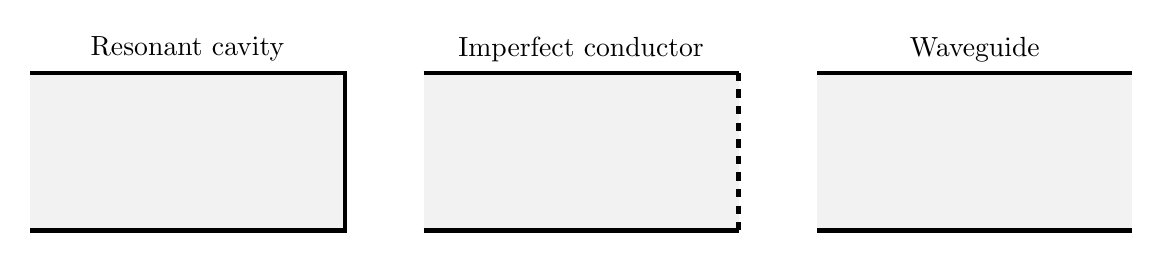
\begin{tikzpicture}
    \node at (2, 2.3) {Resonant cavity};
    \fill[black!5!white] (0, 0) rectangle (4, 2);
    \draw[ultra thick] (0, 0) to (4, 0) to (4, 2) to (0, 2);

    \node at (7, 2.3) {Imperfect conductor};
    \fill[black!5!white] (5, 0) rectangle (9, 2);
    \draw[ultra thick] (5, 0) to (9, 0);
    \draw[ultra thick, dashed] (9, 2) to (9, 0);
    \draw[ultra thick] (5, 2) to (9, 2);

    \node at (12, 2.3) {Waveguide};
    \fill[black!5!white] (10, 0) rectangle (14, 2);
    \draw[ultra thick] (10, 0) to (14, 0);
    \draw[ultra thick] (10, 2) to (14, 2);
\end{tikzpicture}
    \caption{Schematically the most trivial case for each example.}
    \label{fig:examples}
\end{figure}

\subsubsection{Two-dimensional resonant cavity}
\label{subsubsec:cavity}

A resonant cavity is a region $\Omega$ enclosed by a boundary $\partial \Omega$.
The boundary is subdivided into one (or more) inlets $\Gamma_N$ and a perfect
electrically conducting wall $\Gamma_D = \partial \Omega \setminus \Gamma_N$.

\begin{figure}[h]
    \centering
    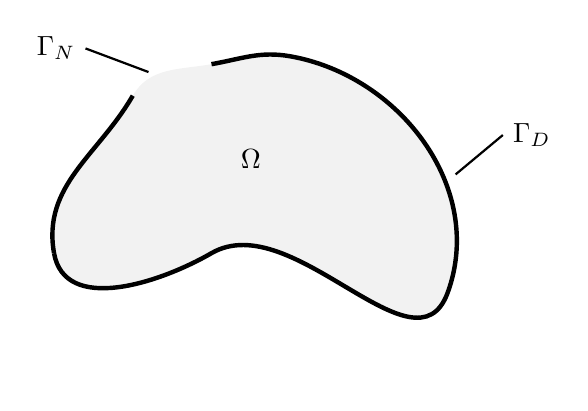
\begin{tikzpicture}
    \fill[black!5!white] (2, 1) to [out=100, in=240] (3, 3)
                              to [out=60, in=190] (4, 3.4)
                              to [out=10, in=170] (5, 3.5)
                              to [out=350, in=70] (7, 0.5)
                              to [out=250, in=30] (4, 1)
                              to [out=210, in=280] (2, 1);
    \draw[ultra thick] (2, 1) to [out=100, in=240] (3, 3);

    \draw[ultra thick] (4, 3.4) to [out=10, in=170] (5, 3.5)
                              to [out=350, in=70] (7, 0.5)
                              to [out=250, in=30] (4, 1)
                              to [out=210, in=280] (2, 1);
    \draw[thick] (2.4, 3.6) node[left] {$\Gamma_N$} to (3.2, 3.3);
    \draw[thick] (7.7, 2.5) node[right] {$\Gamma_D$} to (7.1, 2);
    \node at (4.5, 2.2) {$\Omega$};
\end{tikzpicture}
    \caption{2d resonant cavity.}
    \label{fig:2d-cavity}
\end{figure}

% !REMINDME: Why only need test against v_z?!
Suppose the current density $\mathbf{j} \equiv 0$ and orient the coordinate
system in such a way that $\mathbf{u} = u_z \mathbf{e}_z$ and 
$\mathbf{v} = v_z \mathbf{e}_z$. Consequently,
\begin{equation}
    (\mu^{-1} \nabla \times \mathbf{u}) \cdot (\nabla \times \mathbf{v})
    = (\mu^{-1} \nabla u_z) \cdot (\nabla v_z)
\end{equation}
Use $g_z = (\mathbf{g})_z$ along the boundary $\Gamma_N$,
to convert (\ref{equ:maxwell-weak}) into
the weak formulation for a two-dimensional resonant cavity
\begin{equation}
    \int_{\Omega} (\mu^{-1} \nabla u_z) \cdot (\nabla v_z)
    - \omega^2 \int_{\Omega} \epsilon u_z v_z
    = \int_{\partial \Omega} g_z v_z \label{equ:maxwell-weak-resonant-cavity}
\end{equation}

% Boundary conditions Dirichlet and Neumann (from Monk)
Let $\mathbf{E}$ and $\mathbf{B}$ refer to the electric and magnetic fields inside
the cavity. For now, I distinguish two types of boundaries.

For the perfectly conducting boundary, treated in \citep{monk}, it holds that
\begin{equation}
    \mathbf{n} \times \mathbf{E} = 0,~~\text{on}~\Gamma_D
\end{equation}
For the boundaries in a two-dimensional resonant cavity (see Figure 
\ref{fig:2d-cavity}), this only holds true if $E_z = 0$, which translates
to the Dirichlet boundary condition $\left.\mathbf{u}\right|_{\Gamma_D} = 0$
in light of (\ref{equ:dirichlet-boundary}).

For the inlet, it is easiest to enforce the boundary condition through the
magnetic field $\mathbf{B}$ (considering $\mathbf{n} = -\mathbf{e}_x$ as
depicted in Figure \ref{fig:2d-cavity}):
\begin{equation}
    g_z = (({\mu^{-1} \mathbf{B}}) \times (-\mathbf{e}_x))_z = \mu^{-1} B_x
\end{equation}

\subsubsection{Imperfect conductor}
\label{subsubsec:impedance}

% Additionally impedance boundary condition from Monk
At an imperfect boundary \cite{monk}, (\ref{equ:electricfield}), with (\ref{equ:time-harmonic})
\begin{equation}
    \mathbf{g} = (\mu^{-1} \nabla \times \mathbf{u}) \times \mathbf{n}
    = i \omega \lambda (\mathbf{n} \times \mathbf{u}) \times \mathbf{n}
\end{equation}
which, supposing that $\mathbf{u} = u_z \mathbf{e}_z$ and only treating a
two-dimensional domain, simplifies (using the fact that $\mathbf{n} \perp \mathbf{u}$
and $||\mathbf{n}|| = 1$, so $(\mathbf{n} \times \mathbf{u}) \times \mathbf{n} = \mathbf{u}$)
% !REMINDME: Maybe proof it in appendix
\begin{equation}
    g_z = i \omega \lambda u_z
\end{equation}
Therefore, reuse (\ref{equ:maxwell-weak-resonant-cavity}) as it is, but split 
boundary integral term for Neumann and impedance boundary.

\subsubsection{Waveguide}
\label{subsubsec:waveguide}

We go back to (\ref{equ:maxwell-weak}). Again, $\mathbf{j} \equiv 0$, but now 
we stay in 3d. Supposing that the inlet is located at a constant $x$-value,
such that the surface normal to this inlet is $-\mathbf{e}_x$. For an incoming
magnetic field $\left.\mathbf{B}\right|_{\Gamma_N} = B_0 \mathbf{e}_y$ at the
inlet, we see from (\ref{equ:neumann-boundary}) that $\left.\mathbf{g}\right|_{\Gamma_i}
= - \mu^{-1} B_0 \mathbf{e}_z$. At the outlet, we set $\left.\mathbf{g}\right|_{\Gamma_o} = \boldsymbol{0}$

% Just j=0 and 3d, need to discuss boundary conditions


\pagebreak
\section{Finite element approximation with FEniCS}
\label{sec:fem}

\subsection{Theory (come up with better title)}
\label{subsec:fem-theory}

% Theory

Along the lines of \cite{fenics}.

% WHAT SPACE DO WE WANT V TO BE?!?!
See immediately that the weak formulation (\ref{equ:maxwell-weak}) assumes the shape
\begin{equation}
    \text{Find}~\mathbf{u} \in V,~\text{such that}~a_{\omega}(\mathbf{u}, \mathbf{v}) = L(\mathbf{v}), ~\forall \mathbf{v} \in V_0
\end{equation}
with the bilinear form 
\begin{equation}
    a_{\omega}(\mathbf{u}, \mathbf{v}) = \int_{\Omega} (\mu^{-1} \nabla \times \mathbf{u}) \cdot (\nabla \times \mathbf{v})
    - \omega^2 \int_{\Omega} \epsilon \mathbf{u} \cdot \mathbf{v}
\end{equation}
and the linear form 
\begin{equation}
    L(\mathbf{u}) = \int_{\Omega} \mathbf{j} \cdot \mathbf{v} + \int_{\partial \Omega} \mathbf{g} \cdot \mathbf{v}
\end{equation}

% TO BE CONTINUED WITH GALERKIN STUFF

\subsection{Demonstration (come up with better title)}
\label{subsec:fem-demo}

% Demonstration
In the style of \cite{fenics}. 
Problem (\ref{equ:maxwell-weak}) with $\Omega$ being a cubic cavity with an inlet
on one side and all other sides with $\mu = \epsilon = 0$, $\mathbf{j} = 0$
for simplicity.

Required packages
\lstinputlisting[firstnumber=0, firstline=0, lastline=3]{code/fenics_example.py}

Mesh
\lstinputlisting[firstnumber=5, firstline=6, lastline=7]{code/fenics_example.py}

Function space (Nédélec elements of the first kind \cite{monk})
\lstinputlisting[firstnumber=9, firstline=10, lastline=10]{code/fenics_example.py}

Inlet (at x = 0)
\lstinputlisting[firstnumber=12, firstline=13, lastline=15]{code/fenics_example.py}

PEC boundary
\lstinputlisting[firstnumber=17, firstline=18, lastline=20]{code/fenics_example.py}

Boundary ids
\lstinputlisting[firstnumber=22, firstline=23, lastline=26]{code/fenics_example.py}

Dirichlet boundary (0 for PEC, because Nédélec)
\lstinputlisting[firstnumber=28, firstline=29, lastline=30]{code/fenics_example.py}

Neumann boundary (1 for ...)
\lstinputlisting[firstnumber=32, firstline=33, lastline=34]{code/fenics_example.py}

Trial and test functions
\lstinputlisting[firstnumber=36, firstline=37, lastline=38]{code/fenics_example.py}

Neumann boundary integral term
\lstinputlisting[firstnumber=40, firstline=41, lastline=41]{code/fenics_example.py}

Stiffness matrix
\lstinputlisting[firstnumber=43, firstline=44, lastline=45]{code/fenics_example.py}

Mass matrix
\lstinputlisting[firstnumber=47, firstline=48, lastline=49]{code/fenics_example.py}

L2 norms
\lstinputlisting[firstnumber=51, firstline=52, lastline=54]{code/fenics_example.py}

Solution at frequencies
\lstinputlisting[firstnumber=56, firstline=57, lastline=62]{code/fenics_example.py}

Plotting the L2-norms
\lstinputlisting[firstnumber=64, firstline=65, lastline=66]{code/fenics_example.py}

% Nédelec elements

\pagebreak
\section{Minimal rational interpolation for the time-harmonic Maxwell's equations}
\label{sec:mri}

% General idea 
Let $u : \mathbb{R} \to \mathbb{C}$.
Given $u_j = u(\omega_j)$ for $j \in \{1, \dots, S\}$. Want to find a surrogate
\begin{equation}
    \tilde{u}(\omega) \approx u(\omega)
\end{equation}

\subsection{Motivation}
\label{subsec:motivation}

Equations of the type (\ref{equ:maxwell-timeharmonic}), in the most simple case (dropping
all constants)
\begin{equation}
    \nabla \times (\nabla \times \mathbf{u}) - \omega^2 \mathbf{u} = \mathbf{j}
\end{equation}
Writing the double-curl operator in terms of a matrix $\mathbf{\underline{A}}$
\begin{equation}
    \mathbf{u} = (\mathbf{\underline{A}} - \omega^2)^{-1} \mathbf{j}
\end{equation}
Eigenvalue decomposition $\mathbf{\underline{A}} = \mathbf{\underline{V}} ~ \boldsymbol{\underline{\Lambda}} ~ \mathbf{\underline{V}}^H$
leads us to a form proposed in \cite{helmholtz-motivation}
\begin{equation}
    \mathbf{u} = \mathbf{\underline{V}} (\boldsymbol{\underline{\Lambda}} - \omega^2 \boldsymbol{\underline{1}})^{-1} \mathbf{\underline{V}}^H \mathbf{j} 
    = \sum_i \frac{\mathbf{v}_i \mathbf{v}_i^H \mathbf{j}}{\lambda_i - \omega^2} \label{equ:motivation}
    %= \sum_i \frac{\mathbf{r}_i}{\lambda_i - \omega^2} \label{equ:motivation}
\end{equation}
which follows from the fact that $\boldsymbol{\underline{\Lambda}}$ is diagonal,
hence also $(\boldsymbol{\underline{\Lambda}} - \omega^2 \boldsymbol{\underline{1}})^{-1}$.
Here, we denoted the diagonal elements of $\boldsymbol{\underline{\Lambda}}$ with 
$\lambda_i$ (the eigenvalues of $\mathbf{\underline{A}}$) and the columns of
$\mathbf{\underline{V}}$ with $\mathbf{v}_i$ (the eigenvectors of $\mathbf{\underline{A}}$).

% !REMINDME: This is not really phrased academically yet...
Hence, it would make sense to search for an approximation of the solution $\mathbf{u}$
that is able to \enquote{model} the singularities at $\omega^2 = \lambda_i$, e.g.
rational polynomials
\begin{equation}
    \tilde{u}(\omega) = \frac{P(\omega)}{Q(\omega)}
\end{equation}

% Algorithm (last column SVD is definition of MRI, cite Davide)
\citep{greedyMRI}

\begin{algorithm}
    \caption{Minimal rational interpolation} \label{alg:MRI}
    \begin{algorithmic}
    \Require $\omega_1, \dots, \omega_S$
    \Require $U = [u(\omega_1) | \dots | u(\omega_S)]$ \Comment{Snapshot matrix}
    \State Compute $G$ with $g_{ij} = \langle u(\omega_i), u(\omega_j)\rangle_M,~ i, j \in \{1, \dots, S \}$ \Comment{Gramian matrix}
    \State Compute the singular value decomposition $G = V \Sigma V^H$
    \State Define $q = V[:, S]$
    \State Define $\tilde{u}(\omega) = P(\omega) / Q(\omega)$ with $P(\omega) = \sum_{j=1}^S \frac{q_j u(\omega_j)}{\omega - \omega_j}$ and $Q(\omega) = \sum_{j=1}^S \frac{q_j}{\omega - \omega_j}$
\end{algorithmic}
\end{algorithm}

\citep{shortMRI}

\begin{algorithm}
    \caption{Greedy minimal rational interpolation} \label{alg:gMRI}
    \begin{algorithmic}
    \Require $\tau > 0$ \Comment{Relative $L_2$-error tolerance}
    \Require $\Omega_{\mathrm{test}} = \{\omega_i\}_{i=1}^M$ \Comment{Set of candidate support points}
    \Require $a_{\omega}(\mathbf{u}, \mathbf{v}) = L(\mathbf{v})$ \Comment{Finite element formulation of the problem}
    \State Choose $\omega_1, \dots, \omega_t \in \Omega_{\mathrm{test}}$ \Comment{Usually the smallest and largest element}
    \State Remove $\omega_1, \dots, \omega_t$ from $\Omega_{\mathrm{test}}$
    \State Solve $a_{\omega_i}(\mathbf{u}_i, \mathbf{v}) = L(\mathbf{v})$ for $i \in \{1, \dots, t\}$
    \State Build surrogate $\mathbf{\tilde{u}}_t = \mathbf{P}_t(\omega) / Q_t(\omega)$ using the solutions $\mathbf{u}_1, \dots, \mathbf{u}_t$
    \While{$\Omega_{\mathrm{test}} \neq \emptyset$}
        \State $\omega_{t+1} \leftarrow \textrm{argmin}_{\omega \in \Omega_{\mathrm{test}}} |Q_t(\omega)|$
        \State Solve $a_{\omega_{t+1}}(\mathbf{u}_{t+1}, \mathbf{v}) = L(\mathbf{v})$
        \State Build surrogate $\mathbf{\tilde{u}}_{t+1} = \mathbf{P}_{t+1}(\omega) / Q_{t+1}(\omega)$ using the solutions $\mathbf{u}_1, \dots, \mathbf{u}_{t+1}$
        \If{$||\mathbf{u}_{t+1} - \mathbf{\tilde{u}}_{t}(\omega_{t+1})||_M / ||\mathbf{u}_{t+1}||_M < \tau$}
            \Return
        \EndIf
        \State $t \leftarrow t+1$
    \EndWhile
    %\Return $\tilde{A}(\omega) = \sum_i \frac{q_i A(\omega_i)}{\omega - \omega_i} / \sum_i \frac{q_i}{\omega - \omega_i}$
\end{algorithmic}
\end{algorithm}

% Interpolation property (in barycentric expansion, l'Hôpital whatever)
The rational surrogate $\mathbf{\tilde{u}}$ can be rewritten as 
\begin{align}
    \mathbf{\tilde{u}}(\omega)
    &= \sum_{j=1}^S \frac{q_j \mathbf{u}(\omega_j)}{\omega - \omega_j}
    / \sum_{j=1}^S \frac{q_j}{\omega - \omega_j} \notag \\
    &= \sum_{j=1}^S \prod_{\substack{i=0 \\ i \neq j}}^S (\omega - \omega_i) q_j \mathbf{u}(\omega_j)
    / \sum_{j=1}^S \prod_{\substack{i=0 \\ i \neq j}}^S (\omega - \omega_i) q_j
\end{align}
Therefore, if the rational surrogate $\mathbf{\tilde{u}}$ is evaluated at one of the
interpolation nodes $\omega_i$, $\mathbf{u}(\omega_i)$ is recovered.

If the rational surrogate $\mathbf{\tilde{u}}$ is evaluated in a zero
$\bar{\omega}$ of the denominator $Q(\bar{\omega}) = 0$, we observe a pole,
unless $P(\bar{\omega})$ happens to vanish too.

% Rational root finding 

\citep{klein}

Defining 
\begin{equation}
    v_i = (\omega - \omega_i)^{-1}
\end{equation}
and requiring
\begin{equation}
    0 = Q(\omega) = \sum_{i=1}^S q_i v_i(\omega)
\end{equation}
can be equivalently expressed as a generalized eigenvalue problem
\begin{equation}
    \mathbf{\underline{A}} \mathbf{u} = \omega \mathbf{\underline{B}} \mathbf{u}
\end{equation}
with
\begin{equation}
    \mathbf{\underline{A}} = \begin{pmatrix}
        0 & q_1 & q_2 & \dots & q_S \\
        1 & \omega_1 & & & \\
        1 & & \omega_2 & & \\ 
        \vdots & & & \ddots & \\ 
        1 & & & & \omega_S
    \end{pmatrix} ~~\text{and}~~
    \mathbf{\underline{B}} = \begin{pmatrix}
        0 & & & & \\
         & 1 & & & \\
         & & 1 & & \\ 
        \vdots & & & \ddots & \\ 
         & & & & 1
    \end{pmatrix}\label{equ:root-finding}
\end{equation}

% Optimization tweaks

% -> Householder sequential algorithm instead of full Gramian

\citep{householder}

\begin{algorithm}
    \caption{Additive Householder triangularization} \label{alg:householder}
    \begin{algorithmic}
\Require $U[1 \dots s, 1 \dots N]$ \Comment{Next snapshot matrix}
\Require $R[1 \dots S, 1 \dots S]$  \Comment{Previous triangular matrix}
\Require $E[1 \dots S, 1 \dots N]$ \Comment{Previous orthonormal matrix}
\Require $V[1 \dots S, 1 \dots N]$ \Comment{Previous Householder matrix}
\State Extend size of $R$ to $(S + s) \times (S + s)$
\State Extend $E$ with $S$ orthonormal columns to $(S + s) \times N$
\State Extend size of $V$ to $(S + s) \times N$
\For{$j = S+1:S+s$}
    \State $u = U[j]$
    \For{$k = 1:j-1$}
        \State $u \leftarrow u - 2 \langle V[k, :], u \rangle_M V[k, :]$
        \State $R[k, j] \leftarrow \langle E[k, :], u \rangle_M$
        \State $u \leftarrow u - R[k, j] E[k, :]$
    \EndFor
    \State $R[j, j] \leftarrow ||u||_M$
    \State $\alpha \leftarrow \langle E[j, :], u \rangle_M$
    \If{$|\alpha| \neq 0$}
        \State $E[j, :] \leftarrow E[j, :] (-\alpha / |\alpha|)$
    \EndIf 
    \State $V[j, :] \leftarrow R[j, j] E[j, :] - u$
    \State $V[j, :] \leftarrow V[j, :] - \langle E[S+1:j], V[j, :] \rangle_M E[S+1:j, :]$
    \State $\sigma \leftarrow ||V[j, :]||_M$
    \If{$\sigma \neq 0$}
        \State $V[j, :] \leftarrow V[j, :] / \sigma$
    \Else
        \State$V[j, :] \leftarrow E[j, :]$
    \EndIf
\EndFor
\end{algorithmic}
\end{algorithm}

% -> Check stability of build with SVDs
Can check stability with singular values $\sigma_1, \dots, \sigma_S$ in 
$\Sigma$ which we obtain in Algorithm \ref{alg:MRI}. Need smallest singular values
to different from each other. This conditioning can be estimated with the relative
spectral range \cite{davidePHD}
\begin{equation}
    \frac{\sigma_{S-1} - \sigma_S}{\sigma_1 - \sigma_S}
\end{equation}

% -> Model order reduction techniques (u_ring, error computation, ...)
Denote $\mathbf{\underline{U}} = [\mathbf{u}(\omega_1), \dots, \mathbf{u}(\omega_S)]$
snapshot matrix.
Let 
\begin{equation}
    \mathbf{\mathring{u}} = \sum_{j=1}^S \frac{q_j \mathbf{e}_j}{\omega - \omega_j}
    / \sum_{j=1}^S \frac{q_j}{\omega - \omega_j}
\end{equation}

% STUCK HERE (TO BE CONTINUED)

with the canonical basis vectors $\{ \mathbf{e}_j \}_j$.
If we perform a QR decomposition on this matrix, we obtain 
\begin{equation}
    \mathbf{\underline{U}} = \mathbf{\underline{W}} ~ \mathbf{\underline{R}}
\end{equation}


\pagebreak
\section{Examples}
\label{sec:examples}

\subsection{Two-dimensional rectangular cavity}
\label{subsec:examples-rectangularcavity}

\begin{figure}[h]
    \centering
    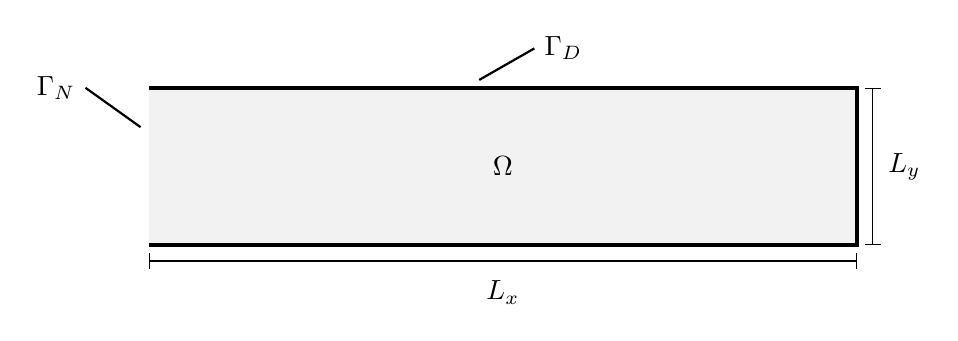
\begin{tikzpicture}
    \fill[black!5!white] (0, 0) rectangle (9, 2);
    \draw[ultra thick] (0, 0) to (9, 0) to (9, 2) to (0, 2);
    \draw[thick] (-0.8, 2) node[left] {$\Gamma_N$} to (-0.1, 1.5);
    \draw[thick] (4.9, 2.5) node[right] {$\Gamma_D$} to (4.2, 2.1);
    \draw[|-|] (0, -0.2) to (9, -0.2);
    \draw[|-|] (9.2, 0) to (9.2, 2);
    \node at (4.5, -0.6) {$L_x$};
    \node at (9.6, 1) {$L_y$};
    \node at (4.5, 1) {$\Omega$};
\end{tikzpicture}

    \caption{TODO.}
    \label{fig:rectangular_cavity}
\end{figure}

% Exploratory plots

\begin{figure}[ht]
    \centering
    \begin{subfigure}{\textwidth}
        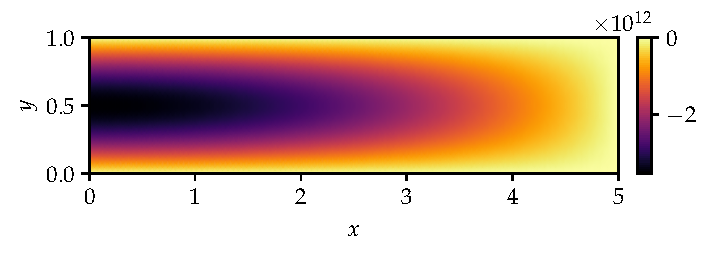
\includegraphics{plots/rectangular_cavity_mode1.pdf}
        \caption{First resonant frequency $\omega = 3.159$.}
    \end{subfigure}
    \begin{subfigure}{\textwidth}
        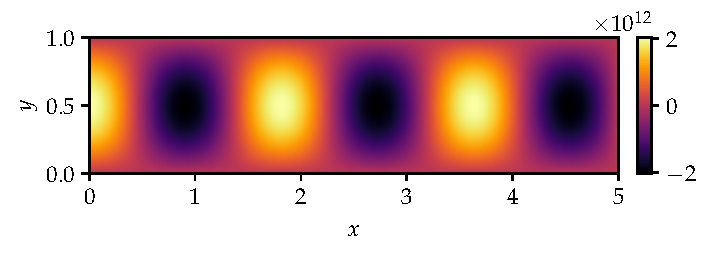
\includegraphics{plots/rectangular_cavity_mode5.pdf}
        \caption{Fifth resonant frequency $\omega = 4.675$.}
    \end{subfigure}
    \caption{Caption.}
    \label{fig:rectangular-cavity-modes}
\end{figure}

% Rational interpolation demonstration
For $||\mathbf{u}||_{L_2(\Omega)}^2 = \int_{\Omega} ||\mathbf{u}||^2$

\begin{figure}[ht]
    \centering
    %% Creator: Matplotlib, PGF backend
%%
%% To include the figure in your LaTeX document, write
%%   \input{<filename>.pgf}
%%
%% Make sure the required packages are loaded in your preamble
%%   \usepackage{pgf}
%%
%% Also ensure that all the required font packages are loaded; for instance,
%% the lmodern package is sometimes necessary when using math font.
%%   \usepackage{lmodern}
%%
%% Figures using additional raster images can only be included by \input if
%% they are in the same directory as the main LaTeX file. For loading figures
%% from other directories you can use the `import` package
%%   \usepackage{import}
%%
%% and then include the figures with
%%   \import{<path to file>}{<filename>.pgf}
%%
%% Matplotlib used the following preamble
%%   \usepackage{fontspec}
%%   \setmainfont{DejaVuSans.ttf}[Path=\detokenize{C:/Users/Fabio/Anaconda3/Lib/site-packages/matplotlib/mpl-data/fonts/ttf/}]
%%   \setsansfont{DejaVuSans.ttf}[Path=\detokenize{C:/Users/Fabio/Anaconda3/Lib/site-packages/matplotlib/mpl-data/fonts/ttf/}]
%%   \setmonofont{DejaVuSansMono.ttf}[Path=\detokenize{C:/Users/Fabio/Anaconda3/Lib/site-packages/matplotlib/mpl-data/fonts/ttf/}]
%%
\begingroup%
\makeatletter%
\begin{pgfpicture}%
\pgfpathrectangle{\pgfpointorigin}{\pgfqpoint{5.180059in}{3.668486in}}%
\pgfusepath{use as bounding box, clip}%
\begin{pgfscope}%
\pgfsetbuttcap%
\pgfsetmiterjoin%
\pgfsetlinewidth{0.000000pt}%
\definecolor{currentstroke}{rgb}{1.000000,1.000000,1.000000}%
\pgfsetstrokecolor{currentstroke}%
\pgfsetstrokeopacity{0.000000}%
\pgfsetdash{}{0pt}%
\pgfpathmoveto{\pgfqpoint{0.000000in}{0.000000in}}%
\pgfpathlineto{\pgfqpoint{5.180059in}{0.000000in}}%
\pgfpathlineto{\pgfqpoint{5.180059in}{3.668486in}}%
\pgfpathlineto{\pgfqpoint{0.000000in}{3.668486in}}%
\pgfpathlineto{\pgfqpoint{0.000000in}{0.000000in}}%
\pgfpathclose%
\pgfusepath{}%
\end{pgfscope}%
\begin{pgfscope}%
\pgfsetbuttcap%
\pgfsetmiterjoin%
\definecolor{currentfill}{rgb}{1.000000,1.000000,1.000000}%
\pgfsetfillcolor{currentfill}%
\pgfsetlinewidth{0.000000pt}%
\definecolor{currentstroke}{rgb}{0.000000,0.000000,0.000000}%
\pgfsetstrokecolor{currentstroke}%
\pgfsetstrokeopacity{0.000000}%
\pgfsetdash{}{0pt}%
\pgfpathmoveto{\pgfqpoint{0.643624in}{2.195759in}}%
\pgfpathlineto{\pgfqpoint{4.944874in}{2.195759in}}%
\pgfpathlineto{\pgfqpoint{4.944874in}{3.568486in}}%
\pgfpathlineto{\pgfqpoint{0.643624in}{3.568486in}}%
\pgfpathlineto{\pgfqpoint{0.643624in}{2.195759in}}%
\pgfpathclose%
\pgfusepath{fill}%
\end{pgfscope}%
\begin{pgfscope}%
\pgfsetbuttcap%
\pgfsetroundjoin%
\definecolor{currentfill}{rgb}{0.000000,0.000000,0.000000}%
\pgfsetfillcolor{currentfill}%
\pgfsetlinewidth{0.803000pt}%
\definecolor{currentstroke}{rgb}{0.000000,0.000000,0.000000}%
\pgfsetstrokecolor{currentstroke}%
\pgfsetdash{}{0pt}%
\pgfsys@defobject{currentmarker}{\pgfqpoint{0.000000in}{-0.048611in}}{\pgfqpoint{0.000000in}{0.000000in}}{%
\pgfpathmoveto{\pgfqpoint{0.000000in}{0.000000in}}%
\pgfpathlineto{\pgfqpoint{0.000000in}{-0.048611in}}%
\pgfusepath{stroke,fill}%
}%
\begin{pgfscope}%
\pgfsys@transformshift{0.643624in}{2.195759in}%
\pgfsys@useobject{currentmarker}{}%
\end{pgfscope}%
\end{pgfscope}%
\begin{pgfscope}%
\pgfsetbuttcap%
\pgfsetroundjoin%
\definecolor{currentfill}{rgb}{0.000000,0.000000,0.000000}%
\pgfsetfillcolor{currentfill}%
\pgfsetlinewidth{0.803000pt}%
\definecolor{currentstroke}{rgb}{0.000000,0.000000,0.000000}%
\pgfsetstrokecolor{currentstroke}%
\pgfsetdash{}{0pt}%
\pgfsys@defobject{currentmarker}{\pgfqpoint{0.000000in}{-0.048611in}}{\pgfqpoint{0.000000in}{0.000000in}}{%
\pgfpathmoveto{\pgfqpoint{0.000000in}{0.000000in}}%
\pgfpathlineto{\pgfqpoint{0.000000in}{-0.048611in}}%
\pgfusepath{stroke,fill}%
}%
\begin{pgfscope}%
\pgfsys@transformshift{1.181280in}{2.195759in}%
\pgfsys@useobject{currentmarker}{}%
\end{pgfscope}%
\end{pgfscope}%
\begin{pgfscope}%
\pgfsetbuttcap%
\pgfsetroundjoin%
\definecolor{currentfill}{rgb}{0.000000,0.000000,0.000000}%
\pgfsetfillcolor{currentfill}%
\pgfsetlinewidth{0.803000pt}%
\definecolor{currentstroke}{rgb}{0.000000,0.000000,0.000000}%
\pgfsetstrokecolor{currentstroke}%
\pgfsetdash{}{0pt}%
\pgfsys@defobject{currentmarker}{\pgfqpoint{0.000000in}{-0.048611in}}{\pgfqpoint{0.000000in}{0.000000in}}{%
\pgfpathmoveto{\pgfqpoint{0.000000in}{0.000000in}}%
\pgfpathlineto{\pgfqpoint{0.000000in}{-0.048611in}}%
\pgfusepath{stroke,fill}%
}%
\begin{pgfscope}%
\pgfsys@transformshift{1.718936in}{2.195759in}%
\pgfsys@useobject{currentmarker}{}%
\end{pgfscope}%
\end{pgfscope}%
\begin{pgfscope}%
\pgfsetbuttcap%
\pgfsetroundjoin%
\definecolor{currentfill}{rgb}{0.000000,0.000000,0.000000}%
\pgfsetfillcolor{currentfill}%
\pgfsetlinewidth{0.803000pt}%
\definecolor{currentstroke}{rgb}{0.000000,0.000000,0.000000}%
\pgfsetstrokecolor{currentstroke}%
\pgfsetdash{}{0pt}%
\pgfsys@defobject{currentmarker}{\pgfqpoint{0.000000in}{-0.048611in}}{\pgfqpoint{0.000000in}{0.000000in}}{%
\pgfpathmoveto{\pgfqpoint{0.000000in}{0.000000in}}%
\pgfpathlineto{\pgfqpoint{0.000000in}{-0.048611in}}%
\pgfusepath{stroke,fill}%
}%
\begin{pgfscope}%
\pgfsys@transformshift{2.256593in}{2.195759in}%
\pgfsys@useobject{currentmarker}{}%
\end{pgfscope}%
\end{pgfscope}%
\begin{pgfscope}%
\pgfsetbuttcap%
\pgfsetroundjoin%
\definecolor{currentfill}{rgb}{0.000000,0.000000,0.000000}%
\pgfsetfillcolor{currentfill}%
\pgfsetlinewidth{0.803000pt}%
\definecolor{currentstroke}{rgb}{0.000000,0.000000,0.000000}%
\pgfsetstrokecolor{currentstroke}%
\pgfsetdash{}{0pt}%
\pgfsys@defobject{currentmarker}{\pgfqpoint{0.000000in}{-0.048611in}}{\pgfqpoint{0.000000in}{0.000000in}}{%
\pgfpathmoveto{\pgfqpoint{0.000000in}{0.000000in}}%
\pgfpathlineto{\pgfqpoint{0.000000in}{-0.048611in}}%
\pgfusepath{stroke,fill}%
}%
\begin{pgfscope}%
\pgfsys@transformshift{2.794249in}{2.195759in}%
\pgfsys@useobject{currentmarker}{}%
\end{pgfscope}%
\end{pgfscope}%
\begin{pgfscope}%
\pgfsetbuttcap%
\pgfsetroundjoin%
\definecolor{currentfill}{rgb}{0.000000,0.000000,0.000000}%
\pgfsetfillcolor{currentfill}%
\pgfsetlinewidth{0.803000pt}%
\definecolor{currentstroke}{rgb}{0.000000,0.000000,0.000000}%
\pgfsetstrokecolor{currentstroke}%
\pgfsetdash{}{0pt}%
\pgfsys@defobject{currentmarker}{\pgfqpoint{0.000000in}{-0.048611in}}{\pgfqpoint{0.000000in}{0.000000in}}{%
\pgfpathmoveto{\pgfqpoint{0.000000in}{0.000000in}}%
\pgfpathlineto{\pgfqpoint{0.000000in}{-0.048611in}}%
\pgfusepath{stroke,fill}%
}%
\begin{pgfscope}%
\pgfsys@transformshift{3.331905in}{2.195759in}%
\pgfsys@useobject{currentmarker}{}%
\end{pgfscope}%
\end{pgfscope}%
\begin{pgfscope}%
\pgfsetbuttcap%
\pgfsetroundjoin%
\definecolor{currentfill}{rgb}{0.000000,0.000000,0.000000}%
\pgfsetfillcolor{currentfill}%
\pgfsetlinewidth{0.803000pt}%
\definecolor{currentstroke}{rgb}{0.000000,0.000000,0.000000}%
\pgfsetstrokecolor{currentstroke}%
\pgfsetdash{}{0pt}%
\pgfsys@defobject{currentmarker}{\pgfqpoint{0.000000in}{-0.048611in}}{\pgfqpoint{0.000000in}{0.000000in}}{%
\pgfpathmoveto{\pgfqpoint{0.000000in}{0.000000in}}%
\pgfpathlineto{\pgfqpoint{0.000000in}{-0.048611in}}%
\pgfusepath{stroke,fill}%
}%
\begin{pgfscope}%
\pgfsys@transformshift{3.869561in}{2.195759in}%
\pgfsys@useobject{currentmarker}{}%
\end{pgfscope}%
\end{pgfscope}%
\begin{pgfscope}%
\pgfsetbuttcap%
\pgfsetroundjoin%
\definecolor{currentfill}{rgb}{0.000000,0.000000,0.000000}%
\pgfsetfillcolor{currentfill}%
\pgfsetlinewidth{0.803000pt}%
\definecolor{currentstroke}{rgb}{0.000000,0.000000,0.000000}%
\pgfsetstrokecolor{currentstroke}%
\pgfsetdash{}{0pt}%
\pgfsys@defobject{currentmarker}{\pgfqpoint{0.000000in}{-0.048611in}}{\pgfqpoint{0.000000in}{0.000000in}}{%
\pgfpathmoveto{\pgfqpoint{0.000000in}{0.000000in}}%
\pgfpathlineto{\pgfqpoint{0.000000in}{-0.048611in}}%
\pgfusepath{stroke,fill}%
}%
\begin{pgfscope}%
\pgfsys@transformshift{4.407218in}{2.195759in}%
\pgfsys@useobject{currentmarker}{}%
\end{pgfscope}%
\end{pgfscope}%
\begin{pgfscope}%
\pgfsetbuttcap%
\pgfsetroundjoin%
\definecolor{currentfill}{rgb}{0.000000,0.000000,0.000000}%
\pgfsetfillcolor{currentfill}%
\pgfsetlinewidth{0.803000pt}%
\definecolor{currentstroke}{rgb}{0.000000,0.000000,0.000000}%
\pgfsetstrokecolor{currentstroke}%
\pgfsetdash{}{0pt}%
\pgfsys@defobject{currentmarker}{\pgfqpoint{0.000000in}{-0.048611in}}{\pgfqpoint{0.000000in}{0.000000in}}{%
\pgfpathmoveto{\pgfqpoint{0.000000in}{0.000000in}}%
\pgfpathlineto{\pgfqpoint{0.000000in}{-0.048611in}}%
\pgfusepath{stroke,fill}%
}%
\begin{pgfscope}%
\pgfsys@transformshift{4.944874in}{2.195759in}%
\pgfsys@useobject{currentmarker}{}%
\end{pgfscope}%
\end{pgfscope}%
\begin{pgfscope}%
\pgfpathrectangle{\pgfqpoint{0.643624in}{2.195759in}}{\pgfqpoint{4.301250in}{1.372727in}}%
\pgfusepath{clip}%
\pgfsetrectcap%
\pgfsetroundjoin%
\pgfsetlinewidth{0.803000pt}%
\definecolor{currentstroke}{rgb}{0.690196,0.690196,0.690196}%
\pgfsetstrokecolor{currentstroke}%
\pgfsetdash{}{0pt}%
\pgfpathmoveto{\pgfqpoint{0.643624in}{2.778814in}}%
\pgfpathlineto{\pgfqpoint{4.944874in}{2.778814in}}%
\pgfusepath{stroke}%
\end{pgfscope}%
\begin{pgfscope}%
\pgfsetbuttcap%
\pgfsetroundjoin%
\definecolor{currentfill}{rgb}{0.000000,0.000000,0.000000}%
\pgfsetfillcolor{currentfill}%
\pgfsetlinewidth{0.803000pt}%
\definecolor{currentstroke}{rgb}{0.000000,0.000000,0.000000}%
\pgfsetstrokecolor{currentstroke}%
\pgfsetdash{}{0pt}%
\pgfsys@defobject{currentmarker}{\pgfqpoint{-0.048611in}{0.000000in}}{\pgfqpoint{-0.000000in}{0.000000in}}{%
\pgfpathmoveto{\pgfqpoint{-0.000000in}{0.000000in}}%
\pgfpathlineto{\pgfqpoint{-0.048611in}{0.000000in}}%
\pgfusepath{stroke,fill}%
}%
\begin{pgfscope}%
\pgfsys@transformshift{0.643624in}{2.778814in}%
\pgfsys@useobject{currentmarker}{}%
\end{pgfscope}%
\end{pgfscope}%
\begin{pgfscope}%
\definecolor{textcolor}{rgb}{0.000000,0.000000,0.000000}%
\pgfsetstrokecolor{textcolor}%
\pgfsetfillcolor{textcolor}%
\pgftext[x=0.328345in, y=2.720777in, left, base]{\color{textcolor}\rmfamily\fontsize{11.000000}{13.200000}\selectfont \(\displaystyle {10^{1}}\)}%
\end{pgfscope}%
\begin{pgfscope}%
\pgfpathrectangle{\pgfqpoint{0.643624in}{2.195759in}}{\pgfqpoint{4.301250in}{1.372727in}}%
\pgfusepath{clip}%
\pgfsetrectcap%
\pgfsetroundjoin%
\pgfsetlinewidth{0.803000pt}%
\definecolor{currentstroke}{rgb}{0.690196,0.690196,0.690196}%
\pgfsetstrokecolor{currentstroke}%
\pgfsetdash{}{0pt}%
\pgfpathmoveto{\pgfqpoint{0.643624in}{3.465178in}}%
\pgfpathlineto{\pgfqpoint{4.944874in}{3.465178in}}%
\pgfusepath{stroke}%
\end{pgfscope}%
\begin{pgfscope}%
\pgfsetbuttcap%
\pgfsetroundjoin%
\definecolor{currentfill}{rgb}{0.000000,0.000000,0.000000}%
\pgfsetfillcolor{currentfill}%
\pgfsetlinewidth{0.803000pt}%
\definecolor{currentstroke}{rgb}{0.000000,0.000000,0.000000}%
\pgfsetstrokecolor{currentstroke}%
\pgfsetdash{}{0pt}%
\pgfsys@defobject{currentmarker}{\pgfqpoint{-0.048611in}{0.000000in}}{\pgfqpoint{-0.000000in}{0.000000in}}{%
\pgfpathmoveto{\pgfqpoint{-0.000000in}{0.000000in}}%
\pgfpathlineto{\pgfqpoint{-0.048611in}{0.000000in}}%
\pgfusepath{stroke,fill}%
}%
\begin{pgfscope}%
\pgfsys@transformshift{0.643624in}{3.465178in}%
\pgfsys@useobject{currentmarker}{}%
\end{pgfscope}%
\end{pgfscope}%
\begin{pgfscope}%
\definecolor{textcolor}{rgb}{0.000000,0.000000,0.000000}%
\pgfsetstrokecolor{textcolor}%
\pgfsetfillcolor{textcolor}%
\pgftext[x=0.328345in, y=3.407140in, left, base]{\color{textcolor}\rmfamily\fontsize{11.000000}{13.200000}\selectfont \(\displaystyle {10^{3}}\)}%
\end{pgfscope}%
\begin{pgfscope}%
\definecolor{textcolor}{rgb}{0.000000,0.000000,0.000000}%
\pgfsetstrokecolor{textcolor}%
\pgfsetfillcolor{textcolor}%
\pgftext[x=0.272790in,y=2.882122in,,bottom,rotate=90.000000]{\color{textcolor}\rmfamily\fontsize{11.000000}{13.200000}\selectfont \(\displaystyle ||u(\omega)||_{L_2(\Omega)}\)}%
\end{pgfscope}%
\begin{pgfscope}%
\pgfpathrectangle{\pgfqpoint{0.643624in}{2.195759in}}{\pgfqpoint{4.301250in}{1.372727in}}%
\pgfusepath{clip}%
\pgfsetrectcap%
\pgfsetroundjoin%
\pgfsetlinewidth{1.505625pt}%
\definecolor{currentstroke}{rgb}{0.001462,0.000466,0.013866}%
\pgfsetstrokecolor{currentstroke}%
\pgfsetdash{}{0pt}%
\pgfpathmoveto{\pgfqpoint{0.643624in}{2.345949in}}%
\pgfpathlineto{\pgfqpoint{0.695291in}{2.365853in}}%
\pgfpathlineto{\pgfqpoint{0.738346in}{2.385738in}}%
\pgfpathlineto{\pgfqpoint{0.772791in}{2.404671in}}%
\pgfpathlineto{\pgfqpoint{0.802929in}{2.424295in}}%
\pgfpathlineto{\pgfqpoint{0.828763in}{2.444241in}}%
\pgfpathlineto{\pgfqpoint{0.854596in}{2.468223in}}%
\pgfpathlineto{\pgfqpoint{0.876124in}{2.492587in}}%
\pgfpathlineto{\pgfqpoint{0.893346in}{2.516191in}}%
\pgfpathlineto{\pgfqpoint{0.910568in}{2.545108in}}%
\pgfpathlineto{\pgfqpoint{0.923485in}{2.571883in}}%
\pgfpathlineto{\pgfqpoint{0.936402in}{2.605265in}}%
\pgfpathlineto{\pgfqpoint{0.949318in}{2.649267in}}%
\pgfpathlineto{\pgfqpoint{0.957929in}{2.688624in}}%
\pgfpathlineto{\pgfqpoint{0.966541in}{2.742859in}}%
\pgfpathlineto{\pgfqpoint{0.975152in}{2.829861in}}%
\pgfpathlineto{\pgfqpoint{0.979457in}{2.905503in}}%
\pgfpathlineto{\pgfqpoint{0.983763in}{3.067348in}}%
\pgfpathlineto{\pgfqpoint{0.988068in}{3.072782in}}%
\pgfpathlineto{\pgfqpoint{0.992374in}{2.907192in}}%
\pgfpathlineto{\pgfqpoint{1.000985in}{2.780538in}}%
\pgfpathlineto{\pgfqpoint{1.009596in}{2.713424in}}%
\pgfpathlineto{\pgfqpoint{1.018207in}{2.667808in}}%
\pgfpathlineto{\pgfqpoint{1.031124in}{2.619263in}}%
\pgfpathlineto{\pgfqpoint{1.044041in}{2.584374in}}%
\pgfpathlineto{\pgfqpoint{1.056957in}{2.558211in}}%
\pgfpathlineto{\pgfqpoint{1.069874in}{2.538484in}}%
\pgfpathlineto{\pgfqpoint{1.082791in}{2.524025in}}%
\pgfpathlineto{\pgfqpoint{1.095707in}{2.514222in}}%
\pgfpathlineto{\pgfqpoint{1.108624in}{2.508766in}}%
\pgfpathlineto{\pgfqpoint{1.121541in}{2.507520in}}%
\pgfpathlineto{\pgfqpoint{1.134457in}{2.510467in}}%
\pgfpathlineto{\pgfqpoint{1.147374in}{2.517693in}}%
\pgfpathlineto{\pgfqpoint{1.160291in}{2.529429in}}%
\pgfpathlineto{\pgfqpoint{1.173207in}{2.546143in}}%
\pgfpathlineto{\pgfqpoint{1.186124in}{2.568725in}}%
\pgfpathlineto{\pgfqpoint{1.199041in}{2.598881in}}%
\pgfpathlineto{\pgfqpoint{1.211957in}{2.640101in}}%
\pgfpathlineto{\pgfqpoint{1.220568in}{2.677388in}}%
\pgfpathlineto{\pgfqpoint{1.229179in}{2.728552in}}%
\pgfpathlineto{\pgfqpoint{1.237791in}{2.808591in}}%
\pgfpathlineto{\pgfqpoint{1.242096in}{2.874617in}}%
\pgfpathlineto{\pgfqpoint{1.246402in}{2.996603in}}%
\pgfpathlineto{\pgfqpoint{1.250707in}{3.192332in}}%
\pgfpathlineto{\pgfqpoint{1.255013in}{2.932406in}}%
\pgfpathlineto{\pgfqpoint{1.259318in}{2.842774in}}%
\pgfpathlineto{\pgfqpoint{1.267929in}{2.747005in}}%
\pgfpathlineto{\pgfqpoint{1.276541in}{2.689486in}}%
\pgfpathlineto{\pgfqpoint{1.285152in}{2.648430in}}%
\pgfpathlineto{\pgfqpoint{1.298068in}{2.603093in}}%
\pgfpathlineto{\pgfqpoint{1.310985in}{2.569109in}}%
\pgfpathlineto{\pgfqpoint{1.328207in}{2.534354in}}%
\pgfpathlineto{\pgfqpoint{1.345429in}{2.507410in}}%
\pgfpathlineto{\pgfqpoint{1.362652in}{2.485828in}}%
\pgfpathlineto{\pgfqpoint{1.384179in}{2.464349in}}%
\pgfpathlineto{\pgfqpoint{1.405707in}{2.447574in}}%
\pgfpathlineto{\pgfqpoint{1.427235in}{2.434619in}}%
\pgfpathlineto{\pgfqpoint{1.448763in}{2.424977in}}%
\pgfpathlineto{\pgfqpoint{1.470291in}{2.418370in}}%
\pgfpathlineto{\pgfqpoint{1.491818in}{2.414675in}}%
\pgfpathlineto{\pgfqpoint{1.513346in}{2.413876in}}%
\pgfpathlineto{\pgfqpoint{1.534874in}{2.416045in}}%
\pgfpathlineto{\pgfqpoint{1.556402in}{2.421342in}}%
\pgfpathlineto{\pgfqpoint{1.577929in}{2.430022in}}%
\pgfpathlineto{\pgfqpoint{1.599457in}{2.442482in}}%
\pgfpathlineto{\pgfqpoint{1.616679in}{2.455579in}}%
\pgfpathlineto{\pgfqpoint{1.633902in}{2.471972in}}%
\pgfpathlineto{\pgfqpoint{1.651124in}{2.492410in}}%
\pgfpathlineto{\pgfqpoint{1.668346in}{2.518107in}}%
\pgfpathlineto{\pgfqpoint{1.681263in}{2.542052in}}%
\pgfpathlineto{\pgfqpoint{1.694179in}{2.571668in}}%
\pgfpathlineto{\pgfqpoint{1.707096in}{2.609768in}}%
\pgfpathlineto{\pgfqpoint{1.715707in}{2.642544in}}%
\pgfpathlineto{\pgfqpoint{1.724318in}{2.685113in}}%
\pgfpathlineto{\pgfqpoint{1.732929in}{2.745489in}}%
\pgfpathlineto{\pgfqpoint{1.737235in}{2.788521in}}%
\pgfpathlineto{\pgfqpoint{1.741541in}{2.849420in}}%
\pgfpathlineto{\pgfqpoint{1.745846in}{2.954376in}}%
\pgfpathlineto{\pgfqpoint{1.750152in}{3.514627in}}%
\pgfpathlineto{\pgfqpoint{1.754457in}{2.947504in}}%
\pgfpathlineto{\pgfqpoint{1.758763in}{2.845857in}}%
\pgfpathlineto{\pgfqpoint{1.767374in}{2.743445in}}%
\pgfpathlineto{\pgfqpoint{1.775985in}{2.683438in}}%
\pgfpathlineto{\pgfqpoint{1.784596in}{2.640928in}}%
\pgfpathlineto{\pgfqpoint{1.797513in}{2.594069in}}%
\pgfpathlineto{\pgfqpoint{1.810429in}{2.558851in}}%
\pgfpathlineto{\pgfqpoint{1.827652in}{2.522581in}}%
\pgfpathlineto{\pgfqpoint{1.844874in}{2.494115in}}%
\pgfpathlineto{\pgfqpoint{1.862096in}{2.470915in}}%
\pgfpathlineto{\pgfqpoint{1.883624in}{2.447181in}}%
\pgfpathlineto{\pgfqpoint{1.905152in}{2.427778in}}%
\pgfpathlineto{\pgfqpoint{1.930985in}{2.408812in}}%
\pgfpathlineto{\pgfqpoint{1.956818in}{2.393553in}}%
\pgfpathlineto{\pgfqpoint{1.986957in}{2.379553in}}%
\pgfpathlineto{\pgfqpoint{2.017096in}{2.369037in}}%
\pgfpathlineto{\pgfqpoint{2.047235in}{2.361628in}}%
\pgfpathlineto{\pgfqpoint{2.077374in}{2.357131in}}%
\pgfpathlineto{\pgfqpoint{2.107513in}{2.355481in}}%
\pgfpathlineto{\pgfqpoint{2.137652in}{2.356721in}}%
\pgfpathlineto{\pgfqpoint{2.167791in}{2.360988in}}%
\pgfpathlineto{\pgfqpoint{2.197929in}{2.368530in}}%
\pgfpathlineto{\pgfqpoint{2.223763in}{2.377888in}}%
\pgfpathlineto{\pgfqpoint{2.249596in}{2.390293in}}%
\pgfpathlineto{\pgfqpoint{2.275429in}{2.406284in}}%
\pgfpathlineto{\pgfqpoint{2.296957in}{2.422935in}}%
\pgfpathlineto{\pgfqpoint{2.318485in}{2.443387in}}%
\pgfpathlineto{\pgfqpoint{2.340013in}{2.468824in}}%
\pgfpathlineto{\pgfqpoint{2.357235in}{2.494084in}}%
\pgfpathlineto{\pgfqpoint{2.374457in}{2.525627in}}%
\pgfpathlineto{\pgfqpoint{2.387374in}{2.555346in}}%
\pgfpathlineto{\pgfqpoint{2.400291in}{2.593149in}}%
\pgfpathlineto{\pgfqpoint{2.408902in}{2.625369in}}%
\pgfpathlineto{\pgfqpoint{2.417513in}{2.666833in}}%
\pgfpathlineto{\pgfqpoint{2.426124in}{2.724829in}}%
\pgfpathlineto{\pgfqpoint{2.430429in}{2.765444in}}%
\pgfpathlineto{\pgfqpoint{2.434735in}{2.821555in}}%
\pgfpathlineto{\pgfqpoint{2.439041in}{2.912757in}}%
\pgfpathlineto{\pgfqpoint{2.443346in}{3.190334in}}%
\pgfpathlineto{\pgfqpoint{2.447652in}{2.968084in}}%
\pgfpathlineto{\pgfqpoint{2.451957in}{2.848857in}}%
\pgfpathlineto{\pgfqpoint{2.460568in}{2.738197in}}%
\pgfpathlineto{\pgfqpoint{2.469179in}{2.675453in}}%
\pgfpathlineto{\pgfqpoint{2.477791in}{2.631520in}}%
\pgfpathlineto{\pgfqpoint{2.490707in}{2.583379in}}%
\pgfpathlineto{\pgfqpoint{2.503624in}{2.547287in}}%
\pgfpathlineto{\pgfqpoint{2.520846in}{2.510093in}}%
\pgfpathlineto{\pgfqpoint{2.538068in}{2.480804in}}%
\pgfpathlineto{\pgfqpoint{2.559596in}{2.451442in}}%
\pgfpathlineto{\pgfqpoint{2.581124in}{2.427647in}}%
\pgfpathlineto{\pgfqpoint{2.606957in}{2.404305in}}%
\pgfpathlineto{\pgfqpoint{2.632791in}{2.385183in}}%
\pgfpathlineto{\pgfqpoint{2.662929in}{2.366933in}}%
\pgfpathlineto{\pgfqpoint{2.693068in}{2.352148in}}%
\pgfpathlineto{\pgfqpoint{2.727513in}{2.338714in}}%
\pgfpathlineto{\pgfqpoint{2.761957in}{2.328425in}}%
\pgfpathlineto{\pgfqpoint{2.800707in}{2.320174in}}%
\pgfpathlineto{\pgfqpoint{2.839457in}{2.315180in}}%
\pgfpathlineto{\pgfqpoint{2.878207in}{2.313337in}}%
\pgfpathlineto{\pgfqpoint{2.916957in}{2.314677in}}%
\pgfpathlineto{\pgfqpoint{2.955707in}{2.319359in}}%
\pgfpathlineto{\pgfqpoint{2.990152in}{2.326566in}}%
\pgfpathlineto{\pgfqpoint{3.024596in}{2.336982in}}%
\pgfpathlineto{\pgfqpoint{3.054735in}{2.349118in}}%
\pgfpathlineto{\pgfqpoint{3.084874in}{2.364598in}}%
\pgfpathlineto{\pgfqpoint{3.110707in}{2.381099in}}%
\pgfpathlineto{\pgfqpoint{3.136541in}{2.401352in}}%
\pgfpathlineto{\pgfqpoint{3.158068in}{2.421922in}}%
\pgfpathlineto{\pgfqpoint{3.179596in}{2.446986in}}%
\pgfpathlineto{\pgfqpoint{3.196818in}{2.471456in}}%
\pgfpathlineto{\pgfqpoint{3.214041in}{2.501530in}}%
\pgfpathlineto{\pgfqpoint{3.226957in}{2.529402in}}%
\pgfpathlineto{\pgfqpoint{3.239874in}{2.564172in}}%
\pgfpathlineto{\pgfqpoint{3.252791in}{2.610106in}}%
\pgfpathlineto{\pgfqpoint{3.261402in}{2.651428in}}%
\pgfpathlineto{\pgfqpoint{3.270013in}{2.709063in}}%
\pgfpathlineto{\pgfqpoint{3.274318in}{2.749300in}}%
\pgfpathlineto{\pgfqpoint{3.278624in}{2.804669in}}%
\pgfpathlineto{\pgfqpoint{3.282929in}{2.893863in}}%
\pgfpathlineto{\pgfqpoint{3.287235in}{3.149362in}}%
\pgfpathlineto{\pgfqpoint{3.295846in}{2.837376in}}%
\pgfpathlineto{\pgfqpoint{3.304457in}{2.725139in}}%
\pgfpathlineto{\pgfqpoint{3.313068in}{2.661882in}}%
\pgfpathlineto{\pgfqpoint{3.321679in}{2.617671in}}%
\pgfpathlineto{\pgfqpoint{3.334596in}{2.569254in}}%
\pgfpathlineto{\pgfqpoint{3.347513in}{2.532941in}}%
\pgfpathlineto{\pgfqpoint{3.364735in}{2.495470in}}%
\pgfpathlineto{\pgfqpoint{3.381957in}{2.465895in}}%
\pgfpathlineto{\pgfqpoint{3.403485in}{2.436143in}}%
\pgfpathlineto{\pgfqpoint{3.425013in}{2.411914in}}%
\pgfpathlineto{\pgfqpoint{3.450846in}{2.387986in}}%
\pgfpathlineto{\pgfqpoint{3.476679in}{2.368200in}}%
\pgfpathlineto{\pgfqpoint{3.506818in}{2.349065in}}%
\pgfpathlineto{\pgfqpoint{3.541263in}{2.331232in}}%
\pgfpathlineto{\pgfqpoint{3.575707in}{2.316827in}}%
\pgfpathlineto{\pgfqpoint{3.614457in}{2.303988in}}%
\pgfpathlineto{\pgfqpoint{3.653207in}{2.294203in}}%
\pgfpathlineto{\pgfqpoint{3.696263in}{2.286513in}}%
\pgfpathlineto{\pgfqpoint{3.739318in}{2.281934in}}%
\pgfpathlineto{\pgfqpoint{3.782374in}{2.280367in}}%
\pgfpathlineto{\pgfqpoint{3.825429in}{2.281840in}}%
\pgfpathlineto{\pgfqpoint{3.868485in}{2.286503in}}%
\pgfpathlineto{\pgfqpoint{3.907235in}{2.293658in}}%
\pgfpathlineto{\pgfqpoint{3.945985in}{2.303950in}}%
\pgfpathlineto{\pgfqpoint{3.980429in}{2.316127in}}%
\pgfpathlineto{\pgfqpoint{4.014874in}{2.331691in}}%
\pgfpathlineto{\pgfqpoint{4.045013in}{2.348702in}}%
\pgfpathlineto{\pgfqpoint{4.070846in}{2.366437in}}%
\pgfpathlineto{\pgfqpoint{4.096679in}{2.387907in}}%
\pgfpathlineto{\pgfqpoint{4.118207in}{2.409540in}}%
\pgfpathlineto{\pgfqpoint{4.139735in}{2.435805in}}%
\pgfpathlineto{\pgfqpoint{4.156957in}{2.461452in}}%
\pgfpathlineto{\pgfqpoint{4.174179in}{2.493082in}}%
\pgfpathlineto{\pgfqpoint{4.187096in}{2.522596in}}%
\pgfpathlineto{\pgfqpoint{4.200013in}{2.559816in}}%
\pgfpathlineto{\pgfqpoint{4.212929in}{2.609968in}}%
\pgfpathlineto{\pgfqpoint{4.221541in}{2.656456in}}%
\pgfpathlineto{\pgfqpoint{4.230152in}{2.724629in}}%
\pgfpathlineto{\pgfqpoint{4.234457in}{2.775775in}}%
\pgfpathlineto{\pgfqpoint{4.238763in}{2.854354in}}%
\pgfpathlineto{\pgfqpoint{4.243068in}{3.031187in}}%
\pgfpathlineto{\pgfqpoint{4.247374in}{2.994786in}}%
\pgfpathlineto{\pgfqpoint{4.251679in}{2.842190in}}%
\pgfpathlineto{\pgfqpoint{4.260291in}{2.719238in}}%
\pgfpathlineto{\pgfqpoint{4.268902in}{2.652818in}}%
\pgfpathlineto{\pgfqpoint{4.277513in}{2.607078in}}%
\pgfpathlineto{\pgfqpoint{4.290429in}{2.557414in}}%
\pgfpathlineto{\pgfqpoint{4.303346in}{2.520367in}}%
\pgfpathlineto{\pgfqpoint{4.320568in}{2.482250in}}%
\pgfpathlineto{\pgfqpoint{4.337791in}{2.452206in}}%
\pgfpathlineto{\pgfqpoint{4.359318in}{2.421981in}}%
\pgfpathlineto{\pgfqpoint{4.380846in}{2.397334in}}%
\pgfpathlineto{\pgfqpoint{4.406679in}{2.372930in}}%
\pgfpathlineto{\pgfqpoint{4.432513in}{2.352665in}}%
\pgfpathlineto{\pgfqpoint{4.462652in}{2.332945in}}%
\pgfpathlineto{\pgfqpoint{4.497096in}{2.314387in}}%
\pgfpathlineto{\pgfqpoint{4.535846in}{2.297472in}}%
\pgfpathlineto{\pgfqpoint{4.574596in}{2.283940in}}%
\pgfpathlineto{\pgfqpoint{4.617652in}{2.272213in}}%
\pgfpathlineto{\pgfqpoint{4.660707in}{2.263514in}}%
\pgfpathlineto{\pgfqpoint{4.708068in}{2.257103in}}%
\pgfpathlineto{\pgfqpoint{4.755429in}{2.253811in}}%
\pgfpathlineto{\pgfqpoint{4.802791in}{2.253589in}}%
\pgfpathlineto{\pgfqpoint{4.850152in}{2.256511in}}%
\pgfpathlineto{\pgfqpoint{4.893207in}{2.262067in}}%
\pgfpathlineto{\pgfqpoint{4.936263in}{2.270658in}}%
\pgfpathlineto{\pgfqpoint{4.944874in}{2.272773in}}%
\pgfpathlineto{\pgfqpoint{4.944874in}{2.272773in}}%
\pgfusepath{stroke}%
\end{pgfscope}%
\begin{pgfscope}%
\pgfsetrectcap%
\pgfsetmiterjoin%
\pgfsetlinewidth{0.803000pt}%
\definecolor{currentstroke}{rgb}{0.000000,0.000000,0.000000}%
\pgfsetstrokecolor{currentstroke}%
\pgfsetdash{}{0pt}%
\pgfpathmoveto{\pgfqpoint{0.643624in}{2.195759in}}%
\pgfpathlineto{\pgfqpoint{0.643624in}{3.568486in}}%
\pgfusepath{stroke}%
\end{pgfscope}%
\begin{pgfscope}%
\pgfsetrectcap%
\pgfsetmiterjoin%
\pgfsetlinewidth{0.803000pt}%
\definecolor{currentstroke}{rgb}{0.000000,0.000000,0.000000}%
\pgfsetstrokecolor{currentstroke}%
\pgfsetdash{}{0pt}%
\pgfpathmoveto{\pgfqpoint{4.944874in}{2.195759in}}%
\pgfpathlineto{\pgfqpoint{4.944874in}{3.568486in}}%
\pgfusepath{stroke}%
\end{pgfscope}%
\begin{pgfscope}%
\pgfsetrectcap%
\pgfsetmiterjoin%
\pgfsetlinewidth{0.803000pt}%
\definecolor{currentstroke}{rgb}{0.000000,0.000000,0.000000}%
\pgfsetstrokecolor{currentstroke}%
\pgfsetdash{}{0pt}%
\pgfpathmoveto{\pgfqpoint{0.643624in}{2.195759in}}%
\pgfpathlineto{\pgfqpoint{4.944874in}{2.195759in}}%
\pgfusepath{stroke}%
\end{pgfscope}%
\begin{pgfscope}%
\pgfsetrectcap%
\pgfsetmiterjoin%
\pgfsetlinewidth{0.803000pt}%
\definecolor{currentstroke}{rgb}{0.000000,0.000000,0.000000}%
\pgfsetstrokecolor{currentstroke}%
\pgfsetdash{}{0pt}%
\pgfpathmoveto{\pgfqpoint{0.643624in}{3.568486in}}%
\pgfpathlineto{\pgfqpoint{4.944874in}{3.568486in}}%
\pgfusepath{stroke}%
\end{pgfscope}%
\begin{pgfscope}%
\pgfsetbuttcap%
\pgfsetmiterjoin%
\definecolor{currentfill}{rgb}{1.000000,1.000000,1.000000}%
\pgfsetfillcolor{currentfill}%
\pgfsetlinewidth{0.000000pt}%
\definecolor{currentstroke}{rgb}{0.000000,0.000000,0.000000}%
\pgfsetstrokecolor{currentstroke}%
\pgfsetstrokeopacity{0.000000}%
\pgfsetdash{}{0pt}%
\pgfpathmoveto{\pgfqpoint{0.643624in}{0.823031in}}%
\pgfpathlineto{\pgfqpoint{4.944874in}{0.823031in}}%
\pgfpathlineto{\pgfqpoint{4.944874in}{2.195759in}}%
\pgfpathlineto{\pgfqpoint{0.643624in}{2.195759in}}%
\pgfpathlineto{\pgfqpoint{0.643624in}{0.823031in}}%
\pgfpathclose%
\pgfusepath{fill}%
\end{pgfscope}%
\begin{pgfscope}%
\pgfsetbuttcap%
\pgfsetroundjoin%
\definecolor{currentfill}{rgb}{0.000000,0.000000,0.000000}%
\pgfsetfillcolor{currentfill}%
\pgfsetlinewidth{0.803000pt}%
\definecolor{currentstroke}{rgb}{0.000000,0.000000,0.000000}%
\pgfsetstrokecolor{currentstroke}%
\pgfsetdash{}{0pt}%
\pgfsys@defobject{currentmarker}{\pgfqpoint{0.000000in}{-0.048611in}}{\pgfqpoint{0.000000in}{0.000000in}}{%
\pgfpathmoveto{\pgfqpoint{0.000000in}{0.000000in}}%
\pgfpathlineto{\pgfqpoint{0.000000in}{-0.048611in}}%
\pgfusepath{stroke,fill}%
}%
\begin{pgfscope}%
\pgfsys@transformshift{0.643624in}{0.823031in}%
\pgfsys@useobject{currentmarker}{}%
\end{pgfscope}%
\end{pgfscope}%
\begin{pgfscope}%
\pgfsetbuttcap%
\pgfsetroundjoin%
\definecolor{currentfill}{rgb}{0.000000,0.000000,0.000000}%
\pgfsetfillcolor{currentfill}%
\pgfsetlinewidth{0.803000pt}%
\definecolor{currentstroke}{rgb}{0.000000,0.000000,0.000000}%
\pgfsetstrokecolor{currentstroke}%
\pgfsetdash{}{0pt}%
\pgfsys@defobject{currentmarker}{\pgfqpoint{0.000000in}{-0.048611in}}{\pgfqpoint{0.000000in}{0.000000in}}{%
\pgfpathmoveto{\pgfqpoint{0.000000in}{0.000000in}}%
\pgfpathlineto{\pgfqpoint{0.000000in}{-0.048611in}}%
\pgfusepath{stroke,fill}%
}%
\begin{pgfscope}%
\pgfsys@transformshift{1.181280in}{0.823031in}%
\pgfsys@useobject{currentmarker}{}%
\end{pgfscope}%
\end{pgfscope}%
\begin{pgfscope}%
\pgfsetbuttcap%
\pgfsetroundjoin%
\definecolor{currentfill}{rgb}{0.000000,0.000000,0.000000}%
\pgfsetfillcolor{currentfill}%
\pgfsetlinewidth{0.803000pt}%
\definecolor{currentstroke}{rgb}{0.000000,0.000000,0.000000}%
\pgfsetstrokecolor{currentstroke}%
\pgfsetdash{}{0pt}%
\pgfsys@defobject{currentmarker}{\pgfqpoint{0.000000in}{-0.048611in}}{\pgfqpoint{0.000000in}{0.000000in}}{%
\pgfpathmoveto{\pgfqpoint{0.000000in}{0.000000in}}%
\pgfpathlineto{\pgfqpoint{0.000000in}{-0.048611in}}%
\pgfusepath{stroke,fill}%
}%
\begin{pgfscope}%
\pgfsys@transformshift{1.718936in}{0.823031in}%
\pgfsys@useobject{currentmarker}{}%
\end{pgfscope}%
\end{pgfscope}%
\begin{pgfscope}%
\pgfsetbuttcap%
\pgfsetroundjoin%
\definecolor{currentfill}{rgb}{0.000000,0.000000,0.000000}%
\pgfsetfillcolor{currentfill}%
\pgfsetlinewidth{0.803000pt}%
\definecolor{currentstroke}{rgb}{0.000000,0.000000,0.000000}%
\pgfsetstrokecolor{currentstroke}%
\pgfsetdash{}{0pt}%
\pgfsys@defobject{currentmarker}{\pgfqpoint{0.000000in}{-0.048611in}}{\pgfqpoint{0.000000in}{0.000000in}}{%
\pgfpathmoveto{\pgfqpoint{0.000000in}{0.000000in}}%
\pgfpathlineto{\pgfqpoint{0.000000in}{-0.048611in}}%
\pgfusepath{stroke,fill}%
}%
\begin{pgfscope}%
\pgfsys@transformshift{2.256593in}{0.823031in}%
\pgfsys@useobject{currentmarker}{}%
\end{pgfscope}%
\end{pgfscope}%
\begin{pgfscope}%
\pgfsetbuttcap%
\pgfsetroundjoin%
\definecolor{currentfill}{rgb}{0.000000,0.000000,0.000000}%
\pgfsetfillcolor{currentfill}%
\pgfsetlinewidth{0.803000pt}%
\definecolor{currentstroke}{rgb}{0.000000,0.000000,0.000000}%
\pgfsetstrokecolor{currentstroke}%
\pgfsetdash{}{0pt}%
\pgfsys@defobject{currentmarker}{\pgfqpoint{0.000000in}{-0.048611in}}{\pgfqpoint{0.000000in}{0.000000in}}{%
\pgfpathmoveto{\pgfqpoint{0.000000in}{0.000000in}}%
\pgfpathlineto{\pgfqpoint{0.000000in}{-0.048611in}}%
\pgfusepath{stroke,fill}%
}%
\begin{pgfscope}%
\pgfsys@transformshift{2.794249in}{0.823031in}%
\pgfsys@useobject{currentmarker}{}%
\end{pgfscope}%
\end{pgfscope}%
\begin{pgfscope}%
\pgfsetbuttcap%
\pgfsetroundjoin%
\definecolor{currentfill}{rgb}{0.000000,0.000000,0.000000}%
\pgfsetfillcolor{currentfill}%
\pgfsetlinewidth{0.803000pt}%
\definecolor{currentstroke}{rgb}{0.000000,0.000000,0.000000}%
\pgfsetstrokecolor{currentstroke}%
\pgfsetdash{}{0pt}%
\pgfsys@defobject{currentmarker}{\pgfqpoint{0.000000in}{-0.048611in}}{\pgfqpoint{0.000000in}{0.000000in}}{%
\pgfpathmoveto{\pgfqpoint{0.000000in}{0.000000in}}%
\pgfpathlineto{\pgfqpoint{0.000000in}{-0.048611in}}%
\pgfusepath{stroke,fill}%
}%
\begin{pgfscope}%
\pgfsys@transformshift{3.331905in}{0.823031in}%
\pgfsys@useobject{currentmarker}{}%
\end{pgfscope}%
\end{pgfscope}%
\begin{pgfscope}%
\pgfsetbuttcap%
\pgfsetroundjoin%
\definecolor{currentfill}{rgb}{0.000000,0.000000,0.000000}%
\pgfsetfillcolor{currentfill}%
\pgfsetlinewidth{0.803000pt}%
\definecolor{currentstroke}{rgb}{0.000000,0.000000,0.000000}%
\pgfsetstrokecolor{currentstroke}%
\pgfsetdash{}{0pt}%
\pgfsys@defobject{currentmarker}{\pgfqpoint{0.000000in}{-0.048611in}}{\pgfqpoint{0.000000in}{0.000000in}}{%
\pgfpathmoveto{\pgfqpoint{0.000000in}{0.000000in}}%
\pgfpathlineto{\pgfqpoint{0.000000in}{-0.048611in}}%
\pgfusepath{stroke,fill}%
}%
\begin{pgfscope}%
\pgfsys@transformshift{3.869561in}{0.823031in}%
\pgfsys@useobject{currentmarker}{}%
\end{pgfscope}%
\end{pgfscope}%
\begin{pgfscope}%
\pgfsetbuttcap%
\pgfsetroundjoin%
\definecolor{currentfill}{rgb}{0.000000,0.000000,0.000000}%
\pgfsetfillcolor{currentfill}%
\pgfsetlinewidth{0.803000pt}%
\definecolor{currentstroke}{rgb}{0.000000,0.000000,0.000000}%
\pgfsetstrokecolor{currentstroke}%
\pgfsetdash{}{0pt}%
\pgfsys@defobject{currentmarker}{\pgfqpoint{0.000000in}{-0.048611in}}{\pgfqpoint{0.000000in}{0.000000in}}{%
\pgfpathmoveto{\pgfqpoint{0.000000in}{0.000000in}}%
\pgfpathlineto{\pgfqpoint{0.000000in}{-0.048611in}}%
\pgfusepath{stroke,fill}%
}%
\begin{pgfscope}%
\pgfsys@transformshift{4.407218in}{0.823031in}%
\pgfsys@useobject{currentmarker}{}%
\end{pgfscope}%
\end{pgfscope}%
\begin{pgfscope}%
\pgfsetbuttcap%
\pgfsetroundjoin%
\definecolor{currentfill}{rgb}{0.000000,0.000000,0.000000}%
\pgfsetfillcolor{currentfill}%
\pgfsetlinewidth{0.803000pt}%
\definecolor{currentstroke}{rgb}{0.000000,0.000000,0.000000}%
\pgfsetstrokecolor{currentstroke}%
\pgfsetdash{}{0pt}%
\pgfsys@defobject{currentmarker}{\pgfqpoint{0.000000in}{-0.048611in}}{\pgfqpoint{0.000000in}{0.000000in}}{%
\pgfpathmoveto{\pgfqpoint{0.000000in}{0.000000in}}%
\pgfpathlineto{\pgfqpoint{0.000000in}{-0.048611in}}%
\pgfusepath{stroke,fill}%
}%
\begin{pgfscope}%
\pgfsys@transformshift{4.944874in}{0.823031in}%
\pgfsys@useobject{currentmarker}{}%
\end{pgfscope}%
\end{pgfscope}%
\begin{pgfscope}%
\pgfpathrectangle{\pgfqpoint{0.643624in}{0.823031in}}{\pgfqpoint{4.301250in}{1.372727in}}%
\pgfusepath{clip}%
\pgfsetrectcap%
\pgfsetroundjoin%
\pgfsetlinewidth{0.803000pt}%
\definecolor{currentstroke}{rgb}{0.690196,0.690196,0.690196}%
\pgfsetstrokecolor{currentstroke}%
\pgfsetdash{}{0pt}%
\pgfpathmoveto{\pgfqpoint{0.643624in}{1.406087in}}%
\pgfpathlineto{\pgfqpoint{4.944874in}{1.406087in}}%
\pgfusepath{stroke}%
\end{pgfscope}%
\begin{pgfscope}%
\pgfsetbuttcap%
\pgfsetroundjoin%
\definecolor{currentfill}{rgb}{0.000000,0.000000,0.000000}%
\pgfsetfillcolor{currentfill}%
\pgfsetlinewidth{0.803000pt}%
\definecolor{currentstroke}{rgb}{0.000000,0.000000,0.000000}%
\pgfsetstrokecolor{currentstroke}%
\pgfsetdash{}{0pt}%
\pgfsys@defobject{currentmarker}{\pgfqpoint{-0.048611in}{0.000000in}}{\pgfqpoint{-0.000000in}{0.000000in}}{%
\pgfpathmoveto{\pgfqpoint{-0.000000in}{0.000000in}}%
\pgfpathlineto{\pgfqpoint{-0.048611in}{0.000000in}}%
\pgfusepath{stroke,fill}%
}%
\begin{pgfscope}%
\pgfsys@transformshift{0.643624in}{1.406087in}%
\pgfsys@useobject{currentmarker}{}%
\end{pgfscope}%
\end{pgfscope}%
\begin{pgfscope}%
\definecolor{textcolor}{rgb}{0.000000,0.000000,0.000000}%
\pgfsetstrokecolor{textcolor}%
\pgfsetfillcolor{textcolor}%
\pgftext[x=0.328345in, y=1.348049in, left, base]{\color{textcolor}\rmfamily\fontsize{11.000000}{13.200000}\selectfont \(\displaystyle {10^{1}}\)}%
\end{pgfscope}%
\begin{pgfscope}%
\pgfpathrectangle{\pgfqpoint{0.643624in}{0.823031in}}{\pgfqpoint{4.301250in}{1.372727in}}%
\pgfusepath{clip}%
\pgfsetrectcap%
\pgfsetroundjoin%
\pgfsetlinewidth{0.803000pt}%
\definecolor{currentstroke}{rgb}{0.690196,0.690196,0.690196}%
\pgfsetstrokecolor{currentstroke}%
\pgfsetdash{}{0pt}%
\pgfpathmoveto{\pgfqpoint{0.643624in}{2.092451in}}%
\pgfpathlineto{\pgfqpoint{4.944874in}{2.092451in}}%
\pgfusepath{stroke}%
\end{pgfscope}%
\begin{pgfscope}%
\pgfsetbuttcap%
\pgfsetroundjoin%
\definecolor{currentfill}{rgb}{0.000000,0.000000,0.000000}%
\pgfsetfillcolor{currentfill}%
\pgfsetlinewidth{0.803000pt}%
\definecolor{currentstroke}{rgb}{0.000000,0.000000,0.000000}%
\pgfsetstrokecolor{currentstroke}%
\pgfsetdash{}{0pt}%
\pgfsys@defobject{currentmarker}{\pgfqpoint{-0.048611in}{0.000000in}}{\pgfqpoint{-0.000000in}{0.000000in}}{%
\pgfpathmoveto{\pgfqpoint{-0.000000in}{0.000000in}}%
\pgfpathlineto{\pgfqpoint{-0.048611in}{0.000000in}}%
\pgfusepath{stroke,fill}%
}%
\begin{pgfscope}%
\pgfsys@transformshift{0.643624in}{2.092451in}%
\pgfsys@useobject{currentmarker}{}%
\end{pgfscope}%
\end{pgfscope}%
\begin{pgfscope}%
\definecolor{textcolor}{rgb}{0.000000,0.000000,0.000000}%
\pgfsetstrokecolor{textcolor}%
\pgfsetfillcolor{textcolor}%
\pgftext[x=0.328345in, y=2.034413in, left, base]{\color{textcolor}\rmfamily\fontsize{11.000000}{13.200000}\selectfont \(\displaystyle {10^{3}}\)}%
\end{pgfscope}%
\begin{pgfscope}%
\definecolor{textcolor}{rgb}{0.000000,0.000000,0.000000}%
\pgfsetstrokecolor{textcolor}%
\pgfsetfillcolor{textcolor}%
\pgftext[x=0.272790in,y=1.509395in,,bottom,rotate=90.000000]{\color{textcolor}\rmfamily\fontsize{11.000000}{13.200000}\selectfont \(\displaystyle ||\tilde{u}(\omega)||_{L_2(\Omega)}\)}%
\end{pgfscope}%
\begin{pgfscope}%
\pgfpathrectangle{\pgfqpoint{0.643624in}{0.823031in}}{\pgfqpoint{4.301250in}{1.372727in}}%
\pgfusepath{clip}%
\pgfsetrectcap%
\pgfsetroundjoin%
\pgfsetlinewidth{1.505625pt}%
\definecolor{currentstroke}{rgb}{0.735683,0.215906,0.330245}%
\pgfsetstrokecolor{currentstroke}%
\pgfsetdash{}{0pt}%
\pgfpathmoveto{\pgfqpoint{0.643624in}{0.973221in}}%
\pgfpathlineto{\pgfqpoint{0.695291in}{0.993129in}}%
\pgfpathlineto{\pgfqpoint{0.738346in}{1.013017in}}%
\pgfpathlineto{\pgfqpoint{0.772791in}{1.031952in}}%
\pgfpathlineto{\pgfqpoint{0.802929in}{1.051579in}}%
\pgfpathlineto{\pgfqpoint{0.828763in}{1.071527in}}%
\pgfpathlineto{\pgfqpoint{0.854596in}{1.095511in}}%
\pgfpathlineto{\pgfqpoint{0.876124in}{1.119879in}}%
\pgfpathlineto{\pgfqpoint{0.893346in}{1.143485in}}%
\pgfpathlineto{\pgfqpoint{0.910568in}{1.172407in}}%
\pgfpathlineto{\pgfqpoint{0.923485in}{1.199186in}}%
\pgfpathlineto{\pgfqpoint{0.936402in}{1.232575in}}%
\pgfpathlineto{\pgfqpoint{0.949318in}{1.276588in}}%
\pgfpathlineto{\pgfqpoint{0.957929in}{1.315958in}}%
\pgfpathlineto{\pgfqpoint{0.966541in}{1.370217in}}%
\pgfpathlineto{\pgfqpoint{0.975152in}{1.457282in}}%
\pgfpathlineto{\pgfqpoint{0.979457in}{1.533018in}}%
\pgfpathlineto{\pgfqpoint{0.983763in}{1.695326in}}%
\pgfpathlineto{\pgfqpoint{0.988068in}{1.699340in}}%
\pgfpathlineto{\pgfqpoint{0.992374in}{1.534233in}}%
\pgfpathlineto{\pgfqpoint{1.000985in}{1.407716in}}%
\pgfpathlineto{\pgfqpoint{1.009596in}{1.340639in}}%
\pgfpathlineto{\pgfqpoint{1.018207in}{1.295041in}}%
\pgfpathlineto{\pgfqpoint{1.031124in}{1.246509in}}%
\pgfpathlineto{\pgfqpoint{1.044041in}{1.211628in}}%
\pgfpathlineto{\pgfqpoint{1.056957in}{1.185470in}}%
\pgfpathlineto{\pgfqpoint{1.069874in}{1.165746in}}%
\pgfpathlineto{\pgfqpoint{1.082791in}{1.151289in}}%
\pgfpathlineto{\pgfqpoint{1.095707in}{1.141489in}}%
\pgfpathlineto{\pgfqpoint{1.108624in}{1.136034in}}%
\pgfpathlineto{\pgfqpoint{1.121541in}{1.134789in}}%
\pgfpathlineto{\pgfqpoint{1.134457in}{1.137737in}}%
\pgfpathlineto{\pgfqpoint{1.147374in}{1.144964in}}%
\pgfpathlineto{\pgfqpoint{1.160291in}{1.156700in}}%
\pgfpathlineto{\pgfqpoint{1.173207in}{1.173415in}}%
\pgfpathlineto{\pgfqpoint{1.186124in}{1.195997in}}%
\pgfpathlineto{\pgfqpoint{1.199041in}{1.226154in}}%
\pgfpathlineto{\pgfqpoint{1.211957in}{1.267374in}}%
\pgfpathlineto{\pgfqpoint{1.220568in}{1.304662in}}%
\pgfpathlineto{\pgfqpoint{1.229179in}{1.355826in}}%
\pgfpathlineto{\pgfqpoint{1.237791in}{1.435866in}}%
\pgfpathlineto{\pgfqpoint{1.242096in}{1.501893in}}%
\pgfpathlineto{\pgfqpoint{1.246402in}{1.623882in}}%
\pgfpathlineto{\pgfqpoint{1.250707in}{1.819587in}}%
\pgfpathlineto{\pgfqpoint{1.255013in}{1.559677in}}%
\pgfpathlineto{\pgfqpoint{1.259318in}{1.470046in}}%
\pgfpathlineto{\pgfqpoint{1.267929in}{1.374278in}}%
\pgfpathlineto{\pgfqpoint{1.276541in}{1.316760in}}%
\pgfpathlineto{\pgfqpoint{1.285152in}{1.275704in}}%
\pgfpathlineto{\pgfqpoint{1.298068in}{1.230367in}}%
\pgfpathlineto{\pgfqpoint{1.310985in}{1.196383in}}%
\pgfpathlineto{\pgfqpoint{1.328207in}{1.161628in}}%
\pgfpathlineto{\pgfqpoint{1.345429in}{1.134685in}}%
\pgfpathlineto{\pgfqpoint{1.362652in}{1.113102in}}%
\pgfpathlineto{\pgfqpoint{1.384179in}{1.091624in}}%
\pgfpathlineto{\pgfqpoint{1.405707in}{1.074849in}}%
\pgfpathlineto{\pgfqpoint{1.427235in}{1.061894in}}%
\pgfpathlineto{\pgfqpoint{1.448763in}{1.052251in}}%
\pgfpathlineto{\pgfqpoint{1.470291in}{1.045645in}}%
\pgfpathlineto{\pgfqpoint{1.491818in}{1.041949in}}%
\pgfpathlineto{\pgfqpoint{1.513346in}{1.041150in}}%
\pgfpathlineto{\pgfqpoint{1.534874in}{1.043319in}}%
\pgfpathlineto{\pgfqpoint{1.556402in}{1.048616in}}%
\pgfpathlineto{\pgfqpoint{1.577929in}{1.057296in}}%
\pgfpathlineto{\pgfqpoint{1.599457in}{1.069756in}}%
\pgfpathlineto{\pgfqpoint{1.616679in}{1.082852in}}%
\pgfpathlineto{\pgfqpoint{1.633902in}{1.099246in}}%
\pgfpathlineto{\pgfqpoint{1.651124in}{1.119684in}}%
\pgfpathlineto{\pgfqpoint{1.668346in}{1.145380in}}%
\pgfpathlineto{\pgfqpoint{1.681263in}{1.169325in}}%
\pgfpathlineto{\pgfqpoint{1.694179in}{1.198941in}}%
\pgfpathlineto{\pgfqpoint{1.707096in}{1.237041in}}%
\pgfpathlineto{\pgfqpoint{1.715707in}{1.269817in}}%
\pgfpathlineto{\pgfqpoint{1.724318in}{1.312386in}}%
\pgfpathlineto{\pgfqpoint{1.732929in}{1.372763in}}%
\pgfpathlineto{\pgfqpoint{1.737235in}{1.415795in}}%
\pgfpathlineto{\pgfqpoint{1.741541in}{1.476693in}}%
\pgfpathlineto{\pgfqpoint{1.745846in}{1.581649in}}%
\pgfpathlineto{\pgfqpoint{1.750152in}{2.141900in}}%
\pgfpathlineto{\pgfqpoint{1.754457in}{1.574777in}}%
\pgfpathlineto{\pgfqpoint{1.758763in}{1.473130in}}%
\pgfpathlineto{\pgfqpoint{1.767374in}{1.370718in}}%
\pgfpathlineto{\pgfqpoint{1.775985in}{1.310711in}}%
\pgfpathlineto{\pgfqpoint{1.784596in}{1.268201in}}%
\pgfpathlineto{\pgfqpoint{1.797513in}{1.221342in}}%
\pgfpathlineto{\pgfqpoint{1.810429in}{1.186124in}}%
\pgfpathlineto{\pgfqpoint{1.827652in}{1.149854in}}%
\pgfpathlineto{\pgfqpoint{1.844874in}{1.121388in}}%
\pgfpathlineto{\pgfqpoint{1.862096in}{1.098188in}}%
\pgfpathlineto{\pgfqpoint{1.883624in}{1.074454in}}%
\pgfpathlineto{\pgfqpoint{1.905152in}{1.055051in}}%
\pgfpathlineto{\pgfqpoint{1.930985in}{1.036085in}}%
\pgfpathlineto{\pgfqpoint{1.956818in}{1.020825in}}%
\pgfpathlineto{\pgfqpoint{1.986957in}{1.006825in}}%
\pgfpathlineto{\pgfqpoint{2.017096in}{0.996310in}}%
\pgfpathlineto{\pgfqpoint{2.047235in}{0.988901in}}%
\pgfpathlineto{\pgfqpoint{2.077374in}{0.984403in}}%
\pgfpathlineto{\pgfqpoint{2.107513in}{0.982754in}}%
\pgfpathlineto{\pgfqpoint{2.137652in}{0.983993in}}%
\pgfpathlineto{\pgfqpoint{2.167791in}{0.988261in}}%
\pgfpathlineto{\pgfqpoint{2.197929in}{0.995803in}}%
\pgfpathlineto{\pgfqpoint{2.223763in}{1.005160in}}%
\pgfpathlineto{\pgfqpoint{2.249596in}{1.017566in}}%
\pgfpathlineto{\pgfqpoint{2.275429in}{1.033557in}}%
\pgfpathlineto{\pgfqpoint{2.296957in}{1.050208in}}%
\pgfpathlineto{\pgfqpoint{2.318485in}{1.070660in}}%
\pgfpathlineto{\pgfqpoint{2.340013in}{1.096097in}}%
\pgfpathlineto{\pgfqpoint{2.357235in}{1.121357in}}%
\pgfpathlineto{\pgfqpoint{2.374457in}{1.152900in}}%
\pgfpathlineto{\pgfqpoint{2.387374in}{1.182619in}}%
\pgfpathlineto{\pgfqpoint{2.400291in}{1.220422in}}%
\pgfpathlineto{\pgfqpoint{2.408902in}{1.252642in}}%
\pgfpathlineto{\pgfqpoint{2.417513in}{1.294106in}}%
\pgfpathlineto{\pgfqpoint{2.426124in}{1.352102in}}%
\pgfpathlineto{\pgfqpoint{2.430429in}{1.392717in}}%
\pgfpathlineto{\pgfqpoint{2.434735in}{1.448829in}}%
\pgfpathlineto{\pgfqpoint{2.439041in}{1.540030in}}%
\pgfpathlineto{\pgfqpoint{2.443346in}{1.817606in}}%
\pgfpathlineto{\pgfqpoint{2.447652in}{1.595357in}}%
\pgfpathlineto{\pgfqpoint{2.451957in}{1.476130in}}%
\pgfpathlineto{\pgfqpoint{2.460568in}{1.365470in}}%
\pgfpathlineto{\pgfqpoint{2.469179in}{1.302726in}}%
\pgfpathlineto{\pgfqpoint{2.477791in}{1.258793in}}%
\pgfpathlineto{\pgfqpoint{2.490707in}{1.210652in}}%
\pgfpathlineto{\pgfqpoint{2.503624in}{1.174560in}}%
\pgfpathlineto{\pgfqpoint{2.520846in}{1.137366in}}%
\pgfpathlineto{\pgfqpoint{2.538068in}{1.108077in}}%
\pgfpathlineto{\pgfqpoint{2.559596in}{1.078715in}}%
\pgfpathlineto{\pgfqpoint{2.581124in}{1.054920in}}%
\pgfpathlineto{\pgfqpoint{2.606957in}{1.031579in}}%
\pgfpathlineto{\pgfqpoint{2.632791in}{1.012457in}}%
\pgfpathlineto{\pgfqpoint{2.662929in}{0.994207in}}%
\pgfpathlineto{\pgfqpoint{2.693068in}{0.979421in}}%
\pgfpathlineto{\pgfqpoint{2.727513in}{0.965987in}}%
\pgfpathlineto{\pgfqpoint{2.761957in}{0.955698in}}%
\pgfpathlineto{\pgfqpoint{2.800707in}{0.947447in}}%
\pgfpathlineto{\pgfqpoint{2.839457in}{0.942453in}}%
\pgfpathlineto{\pgfqpoint{2.878207in}{0.940610in}}%
\pgfpathlineto{\pgfqpoint{2.916957in}{0.941949in}}%
\pgfpathlineto{\pgfqpoint{2.955707in}{0.946631in}}%
\pgfpathlineto{\pgfqpoint{2.990152in}{0.953838in}}%
\pgfpathlineto{\pgfqpoint{3.024596in}{0.964253in}}%
\pgfpathlineto{\pgfqpoint{3.054735in}{0.976389in}}%
\pgfpathlineto{\pgfqpoint{3.084874in}{0.991869in}}%
\pgfpathlineto{\pgfqpoint{3.110707in}{1.008370in}}%
\pgfpathlineto{\pgfqpoint{3.136541in}{1.028623in}}%
\pgfpathlineto{\pgfqpoint{3.158068in}{1.049193in}}%
\pgfpathlineto{\pgfqpoint{3.179596in}{1.074256in}}%
\pgfpathlineto{\pgfqpoint{3.196818in}{1.098727in}}%
\pgfpathlineto{\pgfqpoint{3.214041in}{1.128801in}}%
\pgfpathlineto{\pgfqpoint{3.226957in}{1.156672in}}%
\pgfpathlineto{\pgfqpoint{3.239874in}{1.191441in}}%
\pgfpathlineto{\pgfqpoint{3.252791in}{1.237375in}}%
\pgfpathlineto{\pgfqpoint{3.261402in}{1.278697in}}%
\pgfpathlineto{\pgfqpoint{3.270013in}{1.336332in}}%
\pgfpathlineto{\pgfqpoint{3.274318in}{1.376569in}}%
\pgfpathlineto{\pgfqpoint{3.278624in}{1.431937in}}%
\pgfpathlineto{\pgfqpoint{3.282929in}{1.521129in}}%
\pgfpathlineto{\pgfqpoint{3.287235in}{1.776610in}}%
\pgfpathlineto{\pgfqpoint{3.295846in}{1.464649in}}%
\pgfpathlineto{\pgfqpoint{3.304457in}{1.352411in}}%
\pgfpathlineto{\pgfqpoint{3.313068in}{1.289153in}}%
\pgfpathlineto{\pgfqpoint{3.321679in}{1.244942in}}%
\pgfpathlineto{\pgfqpoint{3.334596in}{1.196524in}}%
\pgfpathlineto{\pgfqpoint{3.347513in}{1.160212in}}%
\pgfpathlineto{\pgfqpoint{3.364735in}{1.122740in}}%
\pgfpathlineto{\pgfqpoint{3.381957in}{1.093165in}}%
\pgfpathlineto{\pgfqpoint{3.403485in}{1.063413in}}%
\pgfpathlineto{\pgfqpoint{3.425013in}{1.039184in}}%
\pgfpathlineto{\pgfqpoint{3.450846in}{1.015256in}}%
\pgfpathlineto{\pgfqpoint{3.476679in}{0.995470in}}%
\pgfpathlineto{\pgfqpoint{3.506818in}{0.976335in}}%
\pgfpathlineto{\pgfqpoint{3.541263in}{0.958503in}}%
\pgfpathlineto{\pgfqpoint{3.575707in}{0.944098in}}%
\pgfpathlineto{\pgfqpoint{3.614457in}{0.931260in}}%
\pgfpathlineto{\pgfqpoint{3.653207in}{0.921475in}}%
\pgfpathlineto{\pgfqpoint{3.696263in}{0.913787in}}%
\pgfpathlineto{\pgfqpoint{3.739318in}{0.909209in}}%
\pgfpathlineto{\pgfqpoint{3.782374in}{0.907643in}}%
\pgfpathlineto{\pgfqpoint{3.825429in}{0.909118in}}%
\pgfpathlineto{\pgfqpoint{3.868485in}{0.913782in}}%
\pgfpathlineto{\pgfqpoint{3.907235in}{0.920938in}}%
\pgfpathlineto{\pgfqpoint{3.945985in}{0.931232in}}%
\pgfpathlineto{\pgfqpoint{3.980429in}{0.943410in}}%
\pgfpathlineto{\pgfqpoint{4.014874in}{0.958976in}}%
\pgfpathlineto{\pgfqpoint{4.045013in}{0.975988in}}%
\pgfpathlineto{\pgfqpoint{4.070846in}{0.993724in}}%
\pgfpathlineto{\pgfqpoint{4.096679in}{1.015194in}}%
\pgfpathlineto{\pgfqpoint{4.118207in}{1.036827in}}%
\pgfpathlineto{\pgfqpoint{4.139735in}{1.063094in}}%
\pgfpathlineto{\pgfqpoint{4.156957in}{1.088741in}}%
\pgfpathlineto{\pgfqpoint{4.174179in}{1.120371in}}%
\pgfpathlineto{\pgfqpoint{4.187096in}{1.149885in}}%
\pgfpathlineto{\pgfqpoint{4.200013in}{1.187104in}}%
\pgfpathlineto{\pgfqpoint{4.212929in}{1.237256in}}%
\pgfpathlineto{\pgfqpoint{4.221541in}{1.283743in}}%
\pgfpathlineto{\pgfqpoint{4.230152in}{1.351916in}}%
\pgfpathlineto{\pgfqpoint{4.234457in}{1.403061in}}%
\pgfpathlineto{\pgfqpoint{4.238763in}{1.481638in}}%
\pgfpathlineto{\pgfqpoint{4.243068in}{1.658460in}}%
\pgfpathlineto{\pgfqpoint{4.247374in}{1.622087in}}%
\pgfpathlineto{\pgfqpoint{4.251679in}{1.469482in}}%
\pgfpathlineto{\pgfqpoint{4.260291in}{1.346528in}}%
\pgfpathlineto{\pgfqpoint{4.268902in}{1.280107in}}%
\pgfpathlineto{\pgfqpoint{4.277513in}{1.234366in}}%
\pgfpathlineto{\pgfqpoint{4.290429in}{1.184701in}}%
\pgfpathlineto{\pgfqpoint{4.303346in}{1.147653in}}%
\pgfpathlineto{\pgfqpoint{4.320568in}{1.109535in}}%
\pgfpathlineto{\pgfqpoint{4.337791in}{1.079490in}}%
\pgfpathlineto{\pgfqpoint{4.359318in}{1.049262in}}%
\pgfpathlineto{\pgfqpoint{4.380846in}{1.024613in}}%
\pgfpathlineto{\pgfqpoint{4.406679in}{1.000204in}}%
\pgfpathlineto{\pgfqpoint{4.432513in}{0.979934in}}%
\pgfpathlineto{\pgfqpoint{4.462652in}{0.960207in}}%
\pgfpathlineto{\pgfqpoint{4.497096in}{0.941640in}}%
\pgfpathlineto{\pgfqpoint{4.535846in}{0.924712in}}%
\pgfpathlineto{\pgfqpoint{4.574596in}{0.911165in}}%
\pgfpathlineto{\pgfqpoint{4.617652in}{0.899418in}}%
\pgfpathlineto{\pgfqpoint{4.660707in}{0.890696in}}%
\pgfpathlineto{\pgfqpoint{4.708068in}{0.884260in}}%
\pgfpathlineto{\pgfqpoint{4.755429in}{0.880946in}}%
\pgfpathlineto{\pgfqpoint{4.802791in}{0.880708in}}%
\pgfpathlineto{\pgfqpoint{4.850152in}{0.883634in}}%
\pgfpathlineto{\pgfqpoint{4.893207in}{0.889224in}}%
\pgfpathlineto{\pgfqpoint{4.936263in}{0.897903in}}%
\pgfpathlineto{\pgfqpoint{4.944874in}{0.900046in}}%
\pgfpathlineto{\pgfqpoint{4.944874in}{0.900046in}}%
\pgfusepath{stroke}%
\end{pgfscope}%
\begin{pgfscope}%
\pgfsetrectcap%
\pgfsetmiterjoin%
\pgfsetlinewidth{0.803000pt}%
\definecolor{currentstroke}{rgb}{0.000000,0.000000,0.000000}%
\pgfsetstrokecolor{currentstroke}%
\pgfsetdash{}{0pt}%
\pgfpathmoveto{\pgfqpoint{0.643624in}{0.823031in}}%
\pgfpathlineto{\pgfqpoint{0.643624in}{2.195759in}}%
\pgfusepath{stroke}%
\end{pgfscope}%
\begin{pgfscope}%
\pgfsetrectcap%
\pgfsetmiterjoin%
\pgfsetlinewidth{0.803000pt}%
\definecolor{currentstroke}{rgb}{0.000000,0.000000,0.000000}%
\pgfsetstrokecolor{currentstroke}%
\pgfsetdash{}{0pt}%
\pgfpathmoveto{\pgfqpoint{4.944874in}{0.823031in}}%
\pgfpathlineto{\pgfqpoint{4.944874in}{2.195759in}}%
\pgfusepath{stroke}%
\end{pgfscope}%
\begin{pgfscope}%
\pgfsetrectcap%
\pgfsetmiterjoin%
\pgfsetlinewidth{0.803000pt}%
\definecolor{currentstroke}{rgb}{0.000000,0.000000,0.000000}%
\pgfsetstrokecolor{currentstroke}%
\pgfsetdash{}{0pt}%
\pgfpathmoveto{\pgfqpoint{0.643624in}{0.823031in}}%
\pgfpathlineto{\pgfqpoint{4.944874in}{0.823031in}}%
\pgfusepath{stroke}%
\end{pgfscope}%
\begin{pgfscope}%
\pgfsetrectcap%
\pgfsetmiterjoin%
\pgfsetlinewidth{0.803000pt}%
\definecolor{currentstroke}{rgb}{0.000000,0.000000,0.000000}%
\pgfsetstrokecolor{currentstroke}%
\pgfsetdash{}{0pt}%
\pgfpathmoveto{\pgfqpoint{0.643624in}{2.195759in}}%
\pgfpathlineto{\pgfqpoint{4.944874in}{2.195759in}}%
\pgfusepath{stroke}%
\end{pgfscope}%
\begin{pgfscope}%
\pgfsetbuttcap%
\pgfsetmiterjoin%
\definecolor{currentfill}{rgb}{1.000000,1.000000,1.000000}%
\pgfsetfillcolor{currentfill}%
\pgfsetlinewidth{0.000000pt}%
\definecolor{currentstroke}{rgb}{0.000000,0.000000,0.000000}%
\pgfsetstrokecolor{currentstroke}%
\pgfsetstrokeopacity{0.000000}%
\pgfsetdash{}{0pt}%
\pgfpathmoveto{\pgfqpoint{0.643624in}{0.548486in}}%
\pgfpathlineto{\pgfqpoint{4.944874in}{0.548486in}}%
\pgfpathlineto{\pgfqpoint{4.944874in}{0.823031in}}%
\pgfpathlineto{\pgfqpoint{0.643624in}{0.823031in}}%
\pgfpathlineto{\pgfqpoint{0.643624in}{0.548486in}}%
\pgfpathclose%
\pgfusepath{fill}%
\end{pgfscope}%
\begin{pgfscope}%
\pgfpathrectangle{\pgfqpoint{0.643624in}{0.548486in}}{\pgfqpoint{4.301250in}{0.274545in}}%
\pgfusepath{clip}%
\pgfsetbuttcap%
\pgfsetroundjoin%
\definecolor{currentfill}{rgb}{0.735683,0.215906,0.330245}%
\pgfsetfillcolor{currentfill}%
\pgfsetlinewidth{1.003750pt}%
\definecolor{currentstroke}{rgb}{0.735683,0.215906,0.330245}%
\pgfsetstrokecolor{currentstroke}%
\pgfsetdash{}{0pt}%
\pgfsys@defobject{currentmarker}{\pgfqpoint{-0.021960in}{-0.021960in}}{\pgfqpoint{0.021960in}{0.021960in}}{%
\pgfpathmoveto{\pgfqpoint{0.000000in}{-0.021960in}}%
\pgfpathcurveto{\pgfqpoint{0.005824in}{-0.021960in}}{\pgfqpoint{0.011410in}{-0.019646in}}{\pgfqpoint{0.015528in}{-0.015528in}}%
\pgfpathcurveto{\pgfqpoint{0.019646in}{-0.011410in}}{\pgfqpoint{0.021960in}{-0.005824in}}{\pgfqpoint{0.021960in}{0.000000in}}%
\pgfpathcurveto{\pgfqpoint{0.021960in}{0.005824in}}{\pgfqpoint{0.019646in}{0.011410in}}{\pgfqpoint{0.015528in}{0.015528in}}%
\pgfpathcurveto{\pgfqpoint{0.011410in}{0.019646in}}{\pgfqpoint{0.005824in}{0.021960in}}{\pgfqpoint{0.000000in}{0.021960in}}%
\pgfpathcurveto{\pgfqpoint{-0.005824in}{0.021960in}}{\pgfqpoint{-0.011410in}{0.019646in}}{\pgfqpoint{-0.015528in}{0.015528in}}%
\pgfpathcurveto{\pgfqpoint{-0.019646in}{0.011410in}}{\pgfqpoint{-0.021960in}{0.005824in}}{\pgfqpoint{-0.021960in}{0.000000in}}%
\pgfpathcurveto{\pgfqpoint{-0.021960in}{-0.005824in}}{\pgfqpoint{-0.019646in}{-0.011410in}}{\pgfqpoint{-0.015528in}{-0.015528in}}%
\pgfpathcurveto{\pgfqpoint{-0.011410in}{-0.019646in}}{\pgfqpoint{-0.005824in}{-0.021960in}}{\pgfqpoint{0.000000in}{-0.021960in}}%
\pgfpathlineto{\pgfqpoint{0.000000in}{-0.021960in}}%
\pgfpathclose%
\pgfusepath{stroke,fill}%
}%
\begin{pgfscope}%
\pgfsys@transformshift{0.643624in}{0.685759in}%
\pgfsys@useobject{currentmarker}{}%
\end{pgfscope}%
\begin{pgfscope}%
\pgfsys@transformshift{4.944874in}{0.685759in}%
\pgfsys@useobject{currentmarker}{}%
\end{pgfscope}%
\begin{pgfscope}%
\pgfsys@transformshift{1.190429in}{0.685759in}%
\pgfsys@useobject{currentmarker}{}%
\end{pgfscope}%
\begin{pgfscope}%
\pgfsys@transformshift{1.263624in}{0.685759in}%
\pgfsys@useobject{currentmarker}{}%
\end{pgfscope}%
\begin{pgfscope}%
\pgfsys@transformshift{3.661818in}{0.685759in}%
\pgfsys@useobject{currentmarker}{}%
\end{pgfscope}%
\begin{pgfscope}%
\pgfsys@transformshift{2.839457in}{0.685759in}%
\pgfsys@useobject{currentmarker}{}%
\end{pgfscope}%
\begin{pgfscope}%
\pgfsys@transformshift{2.215152in}{0.685759in}%
\pgfsys@useobject{currentmarker}{}%
\end{pgfscope}%
\begin{pgfscope}%
\pgfsys@transformshift{1.831957in}{0.685759in}%
\pgfsys@useobject{currentmarker}{}%
\end{pgfscope}%
\begin{pgfscope}%
\pgfsys@transformshift{4.415291in}{0.685759in}%
\pgfsys@useobject{currentmarker}{}%
\end{pgfscope}%
\begin{pgfscope}%
\pgfsys@transformshift{3.295846in}{0.685759in}%
\pgfsys@useobject{currentmarker}{}%
\end{pgfscope}%
\begin{pgfscope}%
\pgfsys@transformshift{4.243068in}{0.685759in}%
\pgfsys@useobject{currentmarker}{}%
\end{pgfscope}%
\begin{pgfscope}%
\pgfsys@transformshift{1.750152in}{0.685759in}%
\pgfsys@useobject{currentmarker}{}%
\end{pgfscope}%
\begin{pgfscope}%
\pgfsys@transformshift{2.443346in}{0.685759in}%
\pgfsys@useobject{currentmarker}{}%
\end{pgfscope}%
\end{pgfscope}%
\begin{pgfscope}%
\pgfsetbuttcap%
\pgfsetroundjoin%
\definecolor{currentfill}{rgb}{0.000000,0.000000,0.000000}%
\pgfsetfillcolor{currentfill}%
\pgfsetlinewidth{0.803000pt}%
\definecolor{currentstroke}{rgb}{0.000000,0.000000,0.000000}%
\pgfsetstrokecolor{currentstroke}%
\pgfsetdash{}{0pt}%
\pgfsys@defobject{currentmarker}{\pgfqpoint{0.000000in}{-0.048611in}}{\pgfqpoint{0.000000in}{0.000000in}}{%
\pgfpathmoveto{\pgfqpoint{0.000000in}{0.000000in}}%
\pgfpathlineto{\pgfqpoint{0.000000in}{-0.048611in}}%
\pgfusepath{stroke,fill}%
}%
\begin{pgfscope}%
\pgfsys@transformshift{0.643624in}{0.548486in}%
\pgfsys@useobject{currentmarker}{}%
\end{pgfscope}%
\end{pgfscope}%
\begin{pgfscope}%
\definecolor{textcolor}{rgb}{0.000000,0.000000,0.000000}%
\pgfsetstrokecolor{textcolor}%
\pgfsetfillcolor{textcolor}%
\pgftext[x=0.643624in,y=0.451264in,,top]{\color{textcolor}\rmfamily\fontsize{11.000000}{13.200000}\selectfont \(\displaystyle {3.00}\)}%
\end{pgfscope}%
\begin{pgfscope}%
\pgfsetbuttcap%
\pgfsetroundjoin%
\definecolor{currentfill}{rgb}{0.000000,0.000000,0.000000}%
\pgfsetfillcolor{currentfill}%
\pgfsetlinewidth{0.803000pt}%
\definecolor{currentstroke}{rgb}{0.000000,0.000000,0.000000}%
\pgfsetstrokecolor{currentstroke}%
\pgfsetdash{}{0pt}%
\pgfsys@defobject{currentmarker}{\pgfqpoint{0.000000in}{-0.048611in}}{\pgfqpoint{0.000000in}{0.000000in}}{%
\pgfpathmoveto{\pgfqpoint{0.000000in}{0.000000in}}%
\pgfpathlineto{\pgfqpoint{0.000000in}{-0.048611in}}%
\pgfusepath{stroke,fill}%
}%
\begin{pgfscope}%
\pgfsys@transformshift{1.181280in}{0.548486in}%
\pgfsys@useobject{currentmarker}{}%
\end{pgfscope}%
\end{pgfscope}%
\begin{pgfscope}%
\definecolor{textcolor}{rgb}{0.000000,0.000000,0.000000}%
\pgfsetstrokecolor{textcolor}%
\pgfsetfillcolor{textcolor}%
\pgftext[x=1.181280in,y=0.451264in,,top]{\color{textcolor}\rmfamily\fontsize{11.000000}{13.200000}\selectfont \(\displaystyle {3.25}\)}%
\end{pgfscope}%
\begin{pgfscope}%
\pgfsetbuttcap%
\pgfsetroundjoin%
\definecolor{currentfill}{rgb}{0.000000,0.000000,0.000000}%
\pgfsetfillcolor{currentfill}%
\pgfsetlinewidth{0.803000pt}%
\definecolor{currentstroke}{rgb}{0.000000,0.000000,0.000000}%
\pgfsetstrokecolor{currentstroke}%
\pgfsetdash{}{0pt}%
\pgfsys@defobject{currentmarker}{\pgfqpoint{0.000000in}{-0.048611in}}{\pgfqpoint{0.000000in}{0.000000in}}{%
\pgfpathmoveto{\pgfqpoint{0.000000in}{0.000000in}}%
\pgfpathlineto{\pgfqpoint{0.000000in}{-0.048611in}}%
\pgfusepath{stroke,fill}%
}%
\begin{pgfscope}%
\pgfsys@transformshift{1.718936in}{0.548486in}%
\pgfsys@useobject{currentmarker}{}%
\end{pgfscope}%
\end{pgfscope}%
\begin{pgfscope}%
\definecolor{textcolor}{rgb}{0.000000,0.000000,0.000000}%
\pgfsetstrokecolor{textcolor}%
\pgfsetfillcolor{textcolor}%
\pgftext[x=1.718936in,y=0.451264in,,top]{\color{textcolor}\rmfamily\fontsize{11.000000}{13.200000}\selectfont \(\displaystyle {3.50}\)}%
\end{pgfscope}%
\begin{pgfscope}%
\pgfsetbuttcap%
\pgfsetroundjoin%
\definecolor{currentfill}{rgb}{0.000000,0.000000,0.000000}%
\pgfsetfillcolor{currentfill}%
\pgfsetlinewidth{0.803000pt}%
\definecolor{currentstroke}{rgb}{0.000000,0.000000,0.000000}%
\pgfsetstrokecolor{currentstroke}%
\pgfsetdash{}{0pt}%
\pgfsys@defobject{currentmarker}{\pgfqpoint{0.000000in}{-0.048611in}}{\pgfqpoint{0.000000in}{0.000000in}}{%
\pgfpathmoveto{\pgfqpoint{0.000000in}{0.000000in}}%
\pgfpathlineto{\pgfqpoint{0.000000in}{-0.048611in}}%
\pgfusepath{stroke,fill}%
}%
\begin{pgfscope}%
\pgfsys@transformshift{2.256593in}{0.548486in}%
\pgfsys@useobject{currentmarker}{}%
\end{pgfscope}%
\end{pgfscope}%
\begin{pgfscope}%
\definecolor{textcolor}{rgb}{0.000000,0.000000,0.000000}%
\pgfsetstrokecolor{textcolor}%
\pgfsetfillcolor{textcolor}%
\pgftext[x=2.256593in,y=0.451264in,,top]{\color{textcolor}\rmfamily\fontsize{11.000000}{13.200000}\selectfont \(\displaystyle {3.75}\)}%
\end{pgfscope}%
\begin{pgfscope}%
\pgfsetbuttcap%
\pgfsetroundjoin%
\definecolor{currentfill}{rgb}{0.000000,0.000000,0.000000}%
\pgfsetfillcolor{currentfill}%
\pgfsetlinewidth{0.803000pt}%
\definecolor{currentstroke}{rgb}{0.000000,0.000000,0.000000}%
\pgfsetstrokecolor{currentstroke}%
\pgfsetdash{}{0pt}%
\pgfsys@defobject{currentmarker}{\pgfqpoint{0.000000in}{-0.048611in}}{\pgfqpoint{0.000000in}{0.000000in}}{%
\pgfpathmoveto{\pgfqpoint{0.000000in}{0.000000in}}%
\pgfpathlineto{\pgfqpoint{0.000000in}{-0.048611in}}%
\pgfusepath{stroke,fill}%
}%
\begin{pgfscope}%
\pgfsys@transformshift{2.794249in}{0.548486in}%
\pgfsys@useobject{currentmarker}{}%
\end{pgfscope}%
\end{pgfscope}%
\begin{pgfscope}%
\definecolor{textcolor}{rgb}{0.000000,0.000000,0.000000}%
\pgfsetstrokecolor{textcolor}%
\pgfsetfillcolor{textcolor}%
\pgftext[x=2.794249in,y=0.451264in,,top]{\color{textcolor}\rmfamily\fontsize{11.000000}{13.200000}\selectfont \(\displaystyle {4.00}\)}%
\end{pgfscope}%
\begin{pgfscope}%
\pgfsetbuttcap%
\pgfsetroundjoin%
\definecolor{currentfill}{rgb}{0.000000,0.000000,0.000000}%
\pgfsetfillcolor{currentfill}%
\pgfsetlinewidth{0.803000pt}%
\definecolor{currentstroke}{rgb}{0.000000,0.000000,0.000000}%
\pgfsetstrokecolor{currentstroke}%
\pgfsetdash{}{0pt}%
\pgfsys@defobject{currentmarker}{\pgfqpoint{0.000000in}{-0.048611in}}{\pgfqpoint{0.000000in}{0.000000in}}{%
\pgfpathmoveto{\pgfqpoint{0.000000in}{0.000000in}}%
\pgfpathlineto{\pgfqpoint{0.000000in}{-0.048611in}}%
\pgfusepath{stroke,fill}%
}%
\begin{pgfscope}%
\pgfsys@transformshift{3.331905in}{0.548486in}%
\pgfsys@useobject{currentmarker}{}%
\end{pgfscope}%
\end{pgfscope}%
\begin{pgfscope}%
\definecolor{textcolor}{rgb}{0.000000,0.000000,0.000000}%
\pgfsetstrokecolor{textcolor}%
\pgfsetfillcolor{textcolor}%
\pgftext[x=3.331905in,y=0.451264in,,top]{\color{textcolor}\rmfamily\fontsize{11.000000}{13.200000}\selectfont \(\displaystyle {4.25}\)}%
\end{pgfscope}%
\begin{pgfscope}%
\pgfsetbuttcap%
\pgfsetroundjoin%
\definecolor{currentfill}{rgb}{0.000000,0.000000,0.000000}%
\pgfsetfillcolor{currentfill}%
\pgfsetlinewidth{0.803000pt}%
\definecolor{currentstroke}{rgb}{0.000000,0.000000,0.000000}%
\pgfsetstrokecolor{currentstroke}%
\pgfsetdash{}{0pt}%
\pgfsys@defobject{currentmarker}{\pgfqpoint{0.000000in}{-0.048611in}}{\pgfqpoint{0.000000in}{0.000000in}}{%
\pgfpathmoveto{\pgfqpoint{0.000000in}{0.000000in}}%
\pgfpathlineto{\pgfqpoint{0.000000in}{-0.048611in}}%
\pgfusepath{stroke,fill}%
}%
\begin{pgfscope}%
\pgfsys@transformshift{3.869561in}{0.548486in}%
\pgfsys@useobject{currentmarker}{}%
\end{pgfscope}%
\end{pgfscope}%
\begin{pgfscope}%
\definecolor{textcolor}{rgb}{0.000000,0.000000,0.000000}%
\pgfsetstrokecolor{textcolor}%
\pgfsetfillcolor{textcolor}%
\pgftext[x=3.869561in,y=0.451264in,,top]{\color{textcolor}\rmfamily\fontsize{11.000000}{13.200000}\selectfont \(\displaystyle {4.50}\)}%
\end{pgfscope}%
\begin{pgfscope}%
\pgfsetbuttcap%
\pgfsetroundjoin%
\definecolor{currentfill}{rgb}{0.000000,0.000000,0.000000}%
\pgfsetfillcolor{currentfill}%
\pgfsetlinewidth{0.803000pt}%
\definecolor{currentstroke}{rgb}{0.000000,0.000000,0.000000}%
\pgfsetstrokecolor{currentstroke}%
\pgfsetdash{}{0pt}%
\pgfsys@defobject{currentmarker}{\pgfqpoint{0.000000in}{-0.048611in}}{\pgfqpoint{0.000000in}{0.000000in}}{%
\pgfpathmoveto{\pgfqpoint{0.000000in}{0.000000in}}%
\pgfpathlineto{\pgfqpoint{0.000000in}{-0.048611in}}%
\pgfusepath{stroke,fill}%
}%
\begin{pgfscope}%
\pgfsys@transformshift{4.407218in}{0.548486in}%
\pgfsys@useobject{currentmarker}{}%
\end{pgfscope}%
\end{pgfscope}%
\begin{pgfscope}%
\definecolor{textcolor}{rgb}{0.000000,0.000000,0.000000}%
\pgfsetstrokecolor{textcolor}%
\pgfsetfillcolor{textcolor}%
\pgftext[x=4.407218in,y=0.451264in,,top]{\color{textcolor}\rmfamily\fontsize{11.000000}{13.200000}\selectfont \(\displaystyle {4.75}\)}%
\end{pgfscope}%
\begin{pgfscope}%
\pgfsetbuttcap%
\pgfsetroundjoin%
\definecolor{currentfill}{rgb}{0.000000,0.000000,0.000000}%
\pgfsetfillcolor{currentfill}%
\pgfsetlinewidth{0.803000pt}%
\definecolor{currentstroke}{rgb}{0.000000,0.000000,0.000000}%
\pgfsetstrokecolor{currentstroke}%
\pgfsetdash{}{0pt}%
\pgfsys@defobject{currentmarker}{\pgfqpoint{0.000000in}{-0.048611in}}{\pgfqpoint{0.000000in}{0.000000in}}{%
\pgfpathmoveto{\pgfqpoint{0.000000in}{0.000000in}}%
\pgfpathlineto{\pgfqpoint{0.000000in}{-0.048611in}}%
\pgfusepath{stroke,fill}%
}%
\begin{pgfscope}%
\pgfsys@transformshift{4.944874in}{0.548486in}%
\pgfsys@useobject{currentmarker}{}%
\end{pgfscope}%
\end{pgfscope}%
\begin{pgfscope}%
\definecolor{textcolor}{rgb}{0.000000,0.000000,0.000000}%
\pgfsetstrokecolor{textcolor}%
\pgfsetfillcolor{textcolor}%
\pgftext[x=4.944874in,y=0.451264in,,top]{\color{textcolor}\rmfamily\fontsize{11.000000}{13.200000}\selectfont \(\displaystyle {5.00}\)}%
\end{pgfscope}%
\begin{pgfscope}%
\definecolor{textcolor}{rgb}{0.000000,0.000000,0.000000}%
\pgfsetstrokecolor{textcolor}%
\pgfsetfillcolor{textcolor}%
\pgftext[x=2.794249in,y=0.247854in,,top]{\color{textcolor}\rmfamily\fontsize{11.000000}{13.200000}\selectfont Frequency \(\displaystyle \omega\)}%
\end{pgfscope}%
\begin{pgfscope}%
\pgfsetrectcap%
\pgfsetmiterjoin%
\pgfsetlinewidth{0.803000pt}%
\definecolor{currentstroke}{rgb}{0.000000,0.000000,0.000000}%
\pgfsetstrokecolor{currentstroke}%
\pgfsetdash{}{0pt}%
\pgfpathmoveto{\pgfqpoint{0.643624in}{0.548486in}}%
\pgfpathlineto{\pgfqpoint{0.643624in}{0.823031in}}%
\pgfusepath{stroke}%
\end{pgfscope}%
\begin{pgfscope}%
\pgfsetrectcap%
\pgfsetmiterjoin%
\pgfsetlinewidth{0.803000pt}%
\definecolor{currentstroke}{rgb}{0.000000,0.000000,0.000000}%
\pgfsetstrokecolor{currentstroke}%
\pgfsetdash{}{0pt}%
\pgfpathmoveto{\pgfqpoint{4.944874in}{0.548486in}}%
\pgfpathlineto{\pgfqpoint{4.944874in}{0.823031in}}%
\pgfusepath{stroke}%
\end{pgfscope}%
\begin{pgfscope}%
\pgfsetrectcap%
\pgfsetmiterjoin%
\pgfsetlinewidth{0.803000pt}%
\definecolor{currentstroke}{rgb}{0.000000,0.000000,0.000000}%
\pgfsetstrokecolor{currentstroke}%
\pgfsetdash{}{0pt}%
\pgfpathmoveto{\pgfqpoint{0.643624in}{0.548486in}}%
\pgfpathlineto{\pgfqpoint{4.944874in}{0.548486in}}%
\pgfusepath{stroke}%
\end{pgfscope}%
\begin{pgfscope}%
\pgfsetrectcap%
\pgfsetmiterjoin%
\pgfsetlinewidth{0.803000pt}%
\definecolor{currentstroke}{rgb}{0.000000,0.000000,0.000000}%
\pgfsetstrokecolor{currentstroke}%
\pgfsetdash{}{0pt}%
\pgfpathmoveto{\pgfqpoint{0.643624in}{0.823031in}}%
\pgfpathlineto{\pgfqpoint{4.944874in}{0.823031in}}%
\pgfusepath{stroke}%
\end{pgfscope}%
\end{pgfpicture}%
\makeatother%
\endgroup%

    \caption{Caption.}
    \label{fig:rectangular-cavity-norms}
\end{figure}

\begin{figure}[ht]
    \centering
    %% Creator: Matplotlib, PGF backend
%%
%% To include the figure in your LaTeX document, write
%%   \input{<filename>.pgf}
%%
%% Make sure the required packages are loaded in your preamble
%%   \usepackage{pgf}
%%
%% Also ensure that all the required font packages are loaded; for instance,
%% the lmodern package is sometimes necessary when using math font.
%%   \usepackage{lmodern}
%%
%% Figures using additional raster images can only be included by \input if
%% they are in the same directory as the main LaTeX file. For loading figures
%% from other directories you can use the `import` package
%%   \usepackage{import}
%%
%% and then include the figures with
%%   \import{<path to file>}{<filename>.pgf}
%%
%% Matplotlib used the following preamble
%%   \usepackage{fontspec}
%%   \setmainfont{DejaVuSans.ttf}[Path=\detokenize{C:/Users/Fabio/Anaconda3/Lib/site-packages/matplotlib/mpl-data/fonts/ttf/}]
%%   \setsansfont{DejaVuSans.ttf}[Path=\detokenize{C:/Users/Fabio/Anaconda3/Lib/site-packages/matplotlib/mpl-data/fonts/ttf/}]
%%   \setmonofont{DejaVuSansMono.ttf}[Path=\detokenize{C:/Users/Fabio/Anaconda3/Lib/site-packages/matplotlib/mpl-data/fonts/ttf/}]
%%
\begingroup%
\makeatletter%
\begin{pgfpicture}%
\pgfpathrectangle{\pgfpointorigin}{\pgfqpoint{5.492394in}{3.668486in}}%
\pgfusepath{use as bounding box, clip}%
\begin{pgfscope}%
\pgfsetbuttcap%
\pgfsetmiterjoin%
\pgfsetlinewidth{0.000000pt}%
\definecolor{currentstroke}{rgb}{1.000000,1.000000,1.000000}%
\pgfsetstrokecolor{currentstroke}%
\pgfsetstrokeopacity{0.000000}%
\pgfsetdash{}{0pt}%
\pgfpathmoveto{\pgfqpoint{0.000000in}{0.000000in}}%
\pgfpathlineto{\pgfqpoint{5.492394in}{0.000000in}}%
\pgfpathlineto{\pgfqpoint{5.492394in}{3.668486in}}%
\pgfpathlineto{\pgfqpoint{0.000000in}{3.668486in}}%
\pgfpathlineto{\pgfqpoint{0.000000in}{0.000000in}}%
\pgfpathclose%
\pgfusepath{}%
\end{pgfscope}%
\begin{pgfscope}%
\pgfsetbuttcap%
\pgfsetmiterjoin%
\definecolor{currentfill}{rgb}{1.000000,1.000000,1.000000}%
\pgfsetfillcolor{currentfill}%
\pgfsetlinewidth{0.000000pt}%
\definecolor{currentstroke}{rgb}{0.000000,0.000000,0.000000}%
\pgfsetstrokecolor{currentstroke}%
\pgfsetstrokeopacity{0.000000}%
\pgfsetdash{}{0pt}%
\pgfpathmoveto{\pgfqpoint{0.955959in}{0.823031in}}%
\pgfpathlineto{\pgfqpoint{5.257209in}{0.823031in}}%
\pgfpathlineto{\pgfqpoint{5.257209in}{3.568486in}}%
\pgfpathlineto{\pgfqpoint{0.955959in}{3.568486in}}%
\pgfpathlineto{\pgfqpoint{0.955959in}{0.823031in}}%
\pgfpathclose%
\pgfusepath{fill}%
\end{pgfscope}%
\begin{pgfscope}%
\pgfsetbuttcap%
\pgfsetroundjoin%
\definecolor{currentfill}{rgb}{0.000000,0.000000,0.000000}%
\pgfsetfillcolor{currentfill}%
\pgfsetlinewidth{0.803000pt}%
\definecolor{currentstroke}{rgb}{0.000000,0.000000,0.000000}%
\pgfsetstrokecolor{currentstroke}%
\pgfsetdash{}{0pt}%
\pgfsys@defobject{currentmarker}{\pgfqpoint{0.000000in}{-0.048611in}}{\pgfqpoint{0.000000in}{0.000000in}}{%
\pgfpathmoveto{\pgfqpoint{0.000000in}{0.000000in}}%
\pgfpathlineto{\pgfqpoint{0.000000in}{-0.048611in}}%
\pgfusepath{stroke,fill}%
}%
\begin{pgfscope}%
\pgfsys@transformshift{0.955959in}{0.823031in}%
\pgfsys@useobject{currentmarker}{}%
\end{pgfscope}%
\end{pgfscope}%
\begin{pgfscope}%
\pgfsetbuttcap%
\pgfsetroundjoin%
\definecolor{currentfill}{rgb}{0.000000,0.000000,0.000000}%
\pgfsetfillcolor{currentfill}%
\pgfsetlinewidth{0.803000pt}%
\definecolor{currentstroke}{rgb}{0.000000,0.000000,0.000000}%
\pgfsetstrokecolor{currentstroke}%
\pgfsetdash{}{0pt}%
\pgfsys@defobject{currentmarker}{\pgfqpoint{0.000000in}{-0.048611in}}{\pgfqpoint{0.000000in}{0.000000in}}{%
\pgfpathmoveto{\pgfqpoint{0.000000in}{0.000000in}}%
\pgfpathlineto{\pgfqpoint{0.000000in}{-0.048611in}}%
\pgfusepath{stroke,fill}%
}%
\begin{pgfscope}%
\pgfsys@transformshift{1.493615in}{0.823031in}%
\pgfsys@useobject{currentmarker}{}%
\end{pgfscope}%
\end{pgfscope}%
\begin{pgfscope}%
\pgfsetbuttcap%
\pgfsetroundjoin%
\definecolor{currentfill}{rgb}{0.000000,0.000000,0.000000}%
\pgfsetfillcolor{currentfill}%
\pgfsetlinewidth{0.803000pt}%
\definecolor{currentstroke}{rgb}{0.000000,0.000000,0.000000}%
\pgfsetstrokecolor{currentstroke}%
\pgfsetdash{}{0pt}%
\pgfsys@defobject{currentmarker}{\pgfqpoint{0.000000in}{-0.048611in}}{\pgfqpoint{0.000000in}{0.000000in}}{%
\pgfpathmoveto{\pgfqpoint{0.000000in}{0.000000in}}%
\pgfpathlineto{\pgfqpoint{0.000000in}{-0.048611in}}%
\pgfusepath{stroke,fill}%
}%
\begin{pgfscope}%
\pgfsys@transformshift{2.031271in}{0.823031in}%
\pgfsys@useobject{currentmarker}{}%
\end{pgfscope}%
\end{pgfscope}%
\begin{pgfscope}%
\pgfsetbuttcap%
\pgfsetroundjoin%
\definecolor{currentfill}{rgb}{0.000000,0.000000,0.000000}%
\pgfsetfillcolor{currentfill}%
\pgfsetlinewidth{0.803000pt}%
\definecolor{currentstroke}{rgb}{0.000000,0.000000,0.000000}%
\pgfsetstrokecolor{currentstroke}%
\pgfsetdash{}{0pt}%
\pgfsys@defobject{currentmarker}{\pgfqpoint{0.000000in}{-0.048611in}}{\pgfqpoint{0.000000in}{0.000000in}}{%
\pgfpathmoveto{\pgfqpoint{0.000000in}{0.000000in}}%
\pgfpathlineto{\pgfqpoint{0.000000in}{-0.048611in}}%
\pgfusepath{stroke,fill}%
}%
\begin{pgfscope}%
\pgfsys@transformshift{2.568928in}{0.823031in}%
\pgfsys@useobject{currentmarker}{}%
\end{pgfscope}%
\end{pgfscope}%
\begin{pgfscope}%
\pgfsetbuttcap%
\pgfsetroundjoin%
\definecolor{currentfill}{rgb}{0.000000,0.000000,0.000000}%
\pgfsetfillcolor{currentfill}%
\pgfsetlinewidth{0.803000pt}%
\definecolor{currentstroke}{rgb}{0.000000,0.000000,0.000000}%
\pgfsetstrokecolor{currentstroke}%
\pgfsetdash{}{0pt}%
\pgfsys@defobject{currentmarker}{\pgfqpoint{0.000000in}{-0.048611in}}{\pgfqpoint{0.000000in}{0.000000in}}{%
\pgfpathmoveto{\pgfqpoint{0.000000in}{0.000000in}}%
\pgfpathlineto{\pgfqpoint{0.000000in}{-0.048611in}}%
\pgfusepath{stroke,fill}%
}%
\begin{pgfscope}%
\pgfsys@transformshift{3.106584in}{0.823031in}%
\pgfsys@useobject{currentmarker}{}%
\end{pgfscope}%
\end{pgfscope}%
\begin{pgfscope}%
\pgfsetbuttcap%
\pgfsetroundjoin%
\definecolor{currentfill}{rgb}{0.000000,0.000000,0.000000}%
\pgfsetfillcolor{currentfill}%
\pgfsetlinewidth{0.803000pt}%
\definecolor{currentstroke}{rgb}{0.000000,0.000000,0.000000}%
\pgfsetstrokecolor{currentstroke}%
\pgfsetdash{}{0pt}%
\pgfsys@defobject{currentmarker}{\pgfqpoint{0.000000in}{-0.048611in}}{\pgfqpoint{0.000000in}{0.000000in}}{%
\pgfpathmoveto{\pgfqpoint{0.000000in}{0.000000in}}%
\pgfpathlineto{\pgfqpoint{0.000000in}{-0.048611in}}%
\pgfusepath{stroke,fill}%
}%
\begin{pgfscope}%
\pgfsys@transformshift{3.644240in}{0.823031in}%
\pgfsys@useobject{currentmarker}{}%
\end{pgfscope}%
\end{pgfscope}%
\begin{pgfscope}%
\pgfsetbuttcap%
\pgfsetroundjoin%
\definecolor{currentfill}{rgb}{0.000000,0.000000,0.000000}%
\pgfsetfillcolor{currentfill}%
\pgfsetlinewidth{0.803000pt}%
\definecolor{currentstroke}{rgb}{0.000000,0.000000,0.000000}%
\pgfsetstrokecolor{currentstroke}%
\pgfsetdash{}{0pt}%
\pgfsys@defobject{currentmarker}{\pgfqpoint{0.000000in}{-0.048611in}}{\pgfqpoint{0.000000in}{0.000000in}}{%
\pgfpathmoveto{\pgfqpoint{0.000000in}{0.000000in}}%
\pgfpathlineto{\pgfqpoint{0.000000in}{-0.048611in}}%
\pgfusepath{stroke,fill}%
}%
\begin{pgfscope}%
\pgfsys@transformshift{4.181896in}{0.823031in}%
\pgfsys@useobject{currentmarker}{}%
\end{pgfscope}%
\end{pgfscope}%
\begin{pgfscope}%
\pgfsetbuttcap%
\pgfsetroundjoin%
\definecolor{currentfill}{rgb}{0.000000,0.000000,0.000000}%
\pgfsetfillcolor{currentfill}%
\pgfsetlinewidth{0.803000pt}%
\definecolor{currentstroke}{rgb}{0.000000,0.000000,0.000000}%
\pgfsetstrokecolor{currentstroke}%
\pgfsetdash{}{0pt}%
\pgfsys@defobject{currentmarker}{\pgfqpoint{0.000000in}{-0.048611in}}{\pgfqpoint{0.000000in}{0.000000in}}{%
\pgfpathmoveto{\pgfqpoint{0.000000in}{0.000000in}}%
\pgfpathlineto{\pgfqpoint{0.000000in}{-0.048611in}}%
\pgfusepath{stroke,fill}%
}%
\begin{pgfscope}%
\pgfsys@transformshift{4.719553in}{0.823031in}%
\pgfsys@useobject{currentmarker}{}%
\end{pgfscope}%
\end{pgfscope}%
\begin{pgfscope}%
\pgfsetbuttcap%
\pgfsetroundjoin%
\definecolor{currentfill}{rgb}{0.000000,0.000000,0.000000}%
\pgfsetfillcolor{currentfill}%
\pgfsetlinewidth{0.803000pt}%
\definecolor{currentstroke}{rgb}{0.000000,0.000000,0.000000}%
\pgfsetstrokecolor{currentstroke}%
\pgfsetdash{}{0pt}%
\pgfsys@defobject{currentmarker}{\pgfqpoint{0.000000in}{-0.048611in}}{\pgfqpoint{0.000000in}{0.000000in}}{%
\pgfpathmoveto{\pgfqpoint{0.000000in}{0.000000in}}%
\pgfpathlineto{\pgfqpoint{0.000000in}{-0.048611in}}%
\pgfusepath{stroke,fill}%
}%
\begin{pgfscope}%
\pgfsys@transformshift{5.257209in}{0.823031in}%
\pgfsys@useobject{currentmarker}{}%
\end{pgfscope}%
\end{pgfscope}%
\begin{pgfscope}%
\pgfpathrectangle{\pgfqpoint{0.955959in}{0.823031in}}{\pgfqpoint{4.301250in}{2.745455in}}%
\pgfusepath{clip}%
\pgfsetrectcap%
\pgfsetroundjoin%
\pgfsetlinewidth{0.803000pt}%
\definecolor{currentstroke}{rgb}{0.690196,0.690196,0.690196}%
\pgfsetstrokecolor{currentstroke}%
\pgfsetdash{}{0pt}%
\pgfpathmoveto{\pgfqpoint{0.955959in}{1.162717in}}%
\pgfpathlineto{\pgfqpoint{5.257209in}{1.162717in}}%
\pgfusepath{stroke}%
\end{pgfscope}%
\begin{pgfscope}%
\pgfsetbuttcap%
\pgfsetroundjoin%
\definecolor{currentfill}{rgb}{0.000000,0.000000,0.000000}%
\pgfsetfillcolor{currentfill}%
\pgfsetlinewidth{0.803000pt}%
\definecolor{currentstroke}{rgb}{0.000000,0.000000,0.000000}%
\pgfsetstrokecolor{currentstroke}%
\pgfsetdash{}{0pt}%
\pgfsys@defobject{currentmarker}{\pgfqpoint{-0.048611in}{0.000000in}}{\pgfqpoint{-0.000000in}{0.000000in}}{%
\pgfpathmoveto{\pgfqpoint{-0.000000in}{0.000000in}}%
\pgfpathlineto{\pgfqpoint{-0.048611in}{0.000000in}}%
\pgfusepath{stroke,fill}%
}%
\begin{pgfscope}%
\pgfsys@transformshift{0.955959in}{1.162717in}%
\pgfsys@useobject{currentmarker}{}%
\end{pgfscope}%
\end{pgfscope}%
\begin{pgfscope}%
\definecolor{textcolor}{rgb}{0.000000,0.000000,0.000000}%
\pgfsetstrokecolor{textcolor}%
\pgfsetfillcolor{textcolor}%
\pgftext[x=0.548858in, y=1.104679in, left, base]{\color{textcolor}\rmfamily\fontsize{11.000000}{13.200000}\selectfont \(\displaystyle {10^{-6}}\)}%
\end{pgfscope}%
\begin{pgfscope}%
\pgfpathrectangle{\pgfqpoint{0.955959in}{0.823031in}}{\pgfqpoint{4.301250in}{2.745455in}}%
\pgfusepath{clip}%
\pgfsetrectcap%
\pgfsetroundjoin%
\pgfsetlinewidth{0.803000pt}%
\definecolor{currentstroke}{rgb}{0.690196,0.690196,0.690196}%
\pgfsetstrokecolor{currentstroke}%
\pgfsetdash{}{0pt}%
\pgfpathmoveto{\pgfqpoint{0.955959in}{1.721958in}}%
\pgfpathlineto{\pgfqpoint{5.257209in}{1.721958in}}%
\pgfusepath{stroke}%
\end{pgfscope}%
\begin{pgfscope}%
\pgfsetbuttcap%
\pgfsetroundjoin%
\definecolor{currentfill}{rgb}{0.000000,0.000000,0.000000}%
\pgfsetfillcolor{currentfill}%
\pgfsetlinewidth{0.803000pt}%
\definecolor{currentstroke}{rgb}{0.000000,0.000000,0.000000}%
\pgfsetstrokecolor{currentstroke}%
\pgfsetdash{}{0pt}%
\pgfsys@defobject{currentmarker}{\pgfqpoint{-0.048611in}{0.000000in}}{\pgfqpoint{-0.000000in}{0.000000in}}{%
\pgfpathmoveto{\pgfqpoint{-0.000000in}{0.000000in}}%
\pgfpathlineto{\pgfqpoint{-0.048611in}{0.000000in}}%
\pgfusepath{stroke,fill}%
}%
\begin{pgfscope}%
\pgfsys@transformshift{0.955959in}{1.721958in}%
\pgfsys@useobject{currentmarker}{}%
\end{pgfscope}%
\end{pgfscope}%
\begin{pgfscope}%
\definecolor{textcolor}{rgb}{0.000000,0.000000,0.000000}%
\pgfsetstrokecolor{textcolor}%
\pgfsetfillcolor{textcolor}%
\pgftext[x=0.548858in, y=1.663920in, left, base]{\color{textcolor}\rmfamily\fontsize{11.000000}{13.200000}\selectfont \(\displaystyle {10^{-4}}\)}%
\end{pgfscope}%
\begin{pgfscope}%
\pgfpathrectangle{\pgfqpoint{0.955959in}{0.823031in}}{\pgfqpoint{4.301250in}{2.745455in}}%
\pgfusepath{clip}%
\pgfsetrectcap%
\pgfsetroundjoin%
\pgfsetlinewidth{0.803000pt}%
\definecolor{currentstroke}{rgb}{0.690196,0.690196,0.690196}%
\pgfsetstrokecolor{currentstroke}%
\pgfsetdash{}{0pt}%
\pgfpathmoveto{\pgfqpoint{0.955959in}{2.281199in}}%
\pgfpathlineto{\pgfqpoint{5.257209in}{2.281199in}}%
\pgfusepath{stroke}%
\end{pgfscope}%
\begin{pgfscope}%
\pgfsetbuttcap%
\pgfsetroundjoin%
\definecolor{currentfill}{rgb}{0.000000,0.000000,0.000000}%
\pgfsetfillcolor{currentfill}%
\pgfsetlinewidth{0.803000pt}%
\definecolor{currentstroke}{rgb}{0.000000,0.000000,0.000000}%
\pgfsetstrokecolor{currentstroke}%
\pgfsetdash{}{0pt}%
\pgfsys@defobject{currentmarker}{\pgfqpoint{-0.048611in}{0.000000in}}{\pgfqpoint{-0.000000in}{0.000000in}}{%
\pgfpathmoveto{\pgfqpoint{-0.000000in}{0.000000in}}%
\pgfpathlineto{\pgfqpoint{-0.048611in}{0.000000in}}%
\pgfusepath{stroke,fill}%
}%
\begin{pgfscope}%
\pgfsys@transformshift{0.955959in}{2.281199in}%
\pgfsys@useobject{currentmarker}{}%
\end{pgfscope}%
\end{pgfscope}%
\begin{pgfscope}%
\definecolor{textcolor}{rgb}{0.000000,0.000000,0.000000}%
\pgfsetstrokecolor{textcolor}%
\pgfsetfillcolor{textcolor}%
\pgftext[x=0.548858in, y=2.223161in, left, base]{\color{textcolor}\rmfamily\fontsize{11.000000}{13.200000}\selectfont \(\displaystyle {10^{-2}}\)}%
\end{pgfscope}%
\begin{pgfscope}%
\pgfpathrectangle{\pgfqpoint{0.955959in}{0.823031in}}{\pgfqpoint{4.301250in}{2.745455in}}%
\pgfusepath{clip}%
\pgfsetrectcap%
\pgfsetroundjoin%
\pgfsetlinewidth{0.803000pt}%
\definecolor{currentstroke}{rgb}{0.690196,0.690196,0.690196}%
\pgfsetstrokecolor{currentstroke}%
\pgfsetdash{}{0pt}%
\pgfpathmoveto{\pgfqpoint{0.955959in}{2.840439in}}%
\pgfpathlineto{\pgfqpoint{5.257209in}{2.840439in}}%
\pgfusepath{stroke}%
\end{pgfscope}%
\begin{pgfscope}%
\pgfsetbuttcap%
\pgfsetroundjoin%
\definecolor{currentfill}{rgb}{0.000000,0.000000,0.000000}%
\pgfsetfillcolor{currentfill}%
\pgfsetlinewidth{0.803000pt}%
\definecolor{currentstroke}{rgb}{0.000000,0.000000,0.000000}%
\pgfsetstrokecolor{currentstroke}%
\pgfsetdash{}{0pt}%
\pgfsys@defobject{currentmarker}{\pgfqpoint{-0.048611in}{0.000000in}}{\pgfqpoint{-0.000000in}{0.000000in}}{%
\pgfpathmoveto{\pgfqpoint{-0.000000in}{0.000000in}}%
\pgfpathlineto{\pgfqpoint{-0.048611in}{0.000000in}}%
\pgfusepath{stroke,fill}%
}%
\begin{pgfscope}%
\pgfsys@transformshift{0.955959in}{2.840439in}%
\pgfsys@useobject{currentmarker}{}%
\end{pgfscope}%
\end{pgfscope}%
\begin{pgfscope}%
\definecolor{textcolor}{rgb}{0.000000,0.000000,0.000000}%
\pgfsetstrokecolor{textcolor}%
\pgfsetfillcolor{textcolor}%
\pgftext[x=0.640680in, y=2.782402in, left, base]{\color{textcolor}\rmfamily\fontsize{11.000000}{13.200000}\selectfont \(\displaystyle {10^{0}}\)}%
\end{pgfscope}%
\begin{pgfscope}%
\pgfpathrectangle{\pgfqpoint{0.955959in}{0.823031in}}{\pgfqpoint{4.301250in}{2.745455in}}%
\pgfusepath{clip}%
\pgfsetrectcap%
\pgfsetroundjoin%
\pgfsetlinewidth{0.803000pt}%
\definecolor{currentstroke}{rgb}{0.690196,0.690196,0.690196}%
\pgfsetstrokecolor{currentstroke}%
\pgfsetdash{}{0pt}%
\pgfpathmoveto{\pgfqpoint{0.955959in}{3.399680in}}%
\pgfpathlineto{\pgfqpoint{5.257209in}{3.399680in}}%
\pgfusepath{stroke}%
\end{pgfscope}%
\begin{pgfscope}%
\pgfsetbuttcap%
\pgfsetroundjoin%
\definecolor{currentfill}{rgb}{0.000000,0.000000,0.000000}%
\pgfsetfillcolor{currentfill}%
\pgfsetlinewidth{0.803000pt}%
\definecolor{currentstroke}{rgb}{0.000000,0.000000,0.000000}%
\pgfsetstrokecolor{currentstroke}%
\pgfsetdash{}{0pt}%
\pgfsys@defobject{currentmarker}{\pgfqpoint{-0.048611in}{0.000000in}}{\pgfqpoint{-0.000000in}{0.000000in}}{%
\pgfpathmoveto{\pgfqpoint{-0.000000in}{0.000000in}}%
\pgfpathlineto{\pgfqpoint{-0.048611in}{0.000000in}}%
\pgfusepath{stroke,fill}%
}%
\begin{pgfscope}%
\pgfsys@transformshift{0.955959in}{3.399680in}%
\pgfsys@useobject{currentmarker}{}%
\end{pgfscope}%
\end{pgfscope}%
\begin{pgfscope}%
\definecolor{textcolor}{rgb}{0.000000,0.000000,0.000000}%
\pgfsetstrokecolor{textcolor}%
\pgfsetfillcolor{textcolor}%
\pgftext[x=0.640680in, y=3.341643in, left, base]{\color{textcolor}\rmfamily\fontsize{11.000000}{13.200000}\selectfont \(\displaystyle {10^{2}}\)}%
\end{pgfscope}%
\begin{pgfscope}%
\definecolor{textcolor}{rgb}{0.000000,0.000000,0.000000}%
\pgfsetstrokecolor{textcolor}%
\pgfsetfillcolor{textcolor}%
\pgftext[x=0.493302in,y=2.195759in,,bottom,rotate=90.000000]{\color{textcolor}\rmfamily\fontsize{11.000000}{13.200000}\selectfont \(\displaystyle \frac{||\tilde{u}_S(\omega) - u(\omega)||_{L_2(\Omega)}}{||\tilde{u}_S(\omega)||_{L_2(\Omega)}}\)}%
\end{pgfscope}%
\begin{pgfscope}%
\pgfpathrectangle{\pgfqpoint{0.955959in}{0.823031in}}{\pgfqpoint{4.301250in}{2.745455in}}%
\pgfusepath{clip}%
\pgfsetrectcap%
\pgfsetroundjoin%
\pgfsetlinewidth{1.505625pt}%
\definecolor{currentstroke}{rgb}{0.001462,0.000466,0.013866}%
\pgfsetstrokecolor{currentstroke}%
\pgfsetdash{}{0pt}%
\pgfpathmoveto{\pgfqpoint{0.948790in}{2.282056in}}%
\pgfpathlineto{\pgfqpoint{0.963175in}{2.284193in}}%
\pgfpathlineto{\pgfqpoint{0.977561in}{2.418747in}}%
\pgfpathlineto{\pgfqpoint{0.991946in}{2.482226in}}%
\pgfpathlineto{\pgfqpoint{1.006331in}{2.524662in}}%
\pgfpathlineto{\pgfqpoint{1.020717in}{2.556875in}}%
\pgfpathlineto{\pgfqpoint{1.035102in}{2.583064in}}%
\pgfpathlineto{\pgfqpoint{1.063872in}{2.624795in}}%
\pgfpathlineto{\pgfqpoint{1.092643in}{2.658241in}}%
\pgfpathlineto{\pgfqpoint{1.121414in}{2.687007in}}%
\pgfpathlineto{\pgfqpoint{1.164570in}{2.725473in}}%
\pgfpathlineto{\pgfqpoint{1.294037in}{2.836519in}}%
\pgfpathlineto{\pgfqpoint{1.351578in}{2.891583in}}%
\pgfpathlineto{\pgfqpoint{1.409119in}{2.949970in}}%
\pgfpathlineto{\pgfqpoint{1.437890in}{2.982886in}}%
\pgfpathlineto{\pgfqpoint{1.452275in}{3.003275in}}%
\pgfpathlineto{\pgfqpoint{1.466661in}{3.030326in}}%
\pgfpathlineto{\pgfqpoint{1.481046in}{3.073007in}}%
\pgfpathlineto{\pgfqpoint{1.495431in}{3.168444in}}%
\pgfpathlineto{\pgfqpoint{1.509817in}{3.216981in}}%
\pgfpathlineto{\pgfqpoint{1.524202in}{3.028429in}}%
\pgfpathlineto{\pgfqpoint{1.538587in}{2.932326in}}%
\pgfpathlineto{\pgfqpoint{1.552972in}{2.865872in}}%
\pgfpathlineto{\pgfqpoint{1.567358in}{2.832565in}}%
\pgfpathlineto{\pgfqpoint{1.581743in}{2.829454in}}%
\pgfpathlineto{\pgfqpoint{1.639284in}{2.864542in}}%
\pgfpathlineto{\pgfqpoint{1.668055in}{2.875265in}}%
\pgfpathlineto{\pgfqpoint{1.696825in}{2.882403in}}%
\pgfpathlineto{\pgfqpoint{1.739981in}{2.888627in}}%
\pgfpathlineto{\pgfqpoint{1.783137in}{2.890695in}}%
\pgfpathlineto{\pgfqpoint{1.826293in}{2.889013in}}%
\pgfpathlineto{\pgfqpoint{1.869449in}{2.883733in}}%
\pgfpathlineto{\pgfqpoint{1.912605in}{2.875266in}}%
\pgfpathlineto{\pgfqpoint{1.984531in}{2.857040in}}%
\pgfpathlineto{\pgfqpoint{2.042072in}{2.843774in}}%
\pgfpathlineto{\pgfqpoint{2.085228in}{2.837869in}}%
\pgfpathlineto{\pgfqpoint{2.113999in}{2.836532in}}%
\pgfpathlineto{\pgfqpoint{2.157155in}{2.838179in}}%
\pgfpathlineto{\pgfqpoint{2.214696in}{2.844986in}}%
\pgfpathlineto{\pgfqpoint{2.344163in}{2.863002in}}%
\pgfpathlineto{\pgfqpoint{2.401705in}{2.867686in}}%
\pgfpathlineto{\pgfqpoint{2.459246in}{2.869147in}}%
\pgfpathlineto{\pgfqpoint{2.516787in}{2.867224in}}%
\pgfpathlineto{\pgfqpoint{2.574328in}{2.862236in}}%
\pgfpathlineto{\pgfqpoint{2.675025in}{2.849258in}}%
\pgfpathlineto{\pgfqpoint{2.746952in}{2.841177in}}%
\pgfpathlineto{\pgfqpoint{2.804493in}{2.838381in}}%
\pgfpathlineto{\pgfqpoint{2.847649in}{2.839055in}}%
\pgfpathlineto{\pgfqpoint{2.905190in}{2.843206in}}%
\pgfpathlineto{\pgfqpoint{2.991502in}{2.853283in}}%
\pgfpathlineto{\pgfqpoint{3.106584in}{2.866219in}}%
\pgfpathlineto{\pgfqpoint{3.178510in}{2.871104in}}%
\pgfpathlineto{\pgfqpoint{3.250437in}{2.872506in}}%
\pgfpathlineto{\pgfqpoint{3.322363in}{2.870159in}}%
\pgfpathlineto{\pgfqpoint{3.394290in}{2.864312in}}%
\pgfpathlineto{\pgfqpoint{3.494987in}{2.852208in}}%
\pgfpathlineto{\pgfqpoint{3.595684in}{2.840833in}}%
\pgfpathlineto{\pgfqpoint{3.653225in}{2.837608in}}%
\pgfpathlineto{\pgfqpoint{3.710766in}{2.837960in}}%
\pgfpathlineto{\pgfqpoint{3.768307in}{2.841692in}}%
\pgfpathlineto{\pgfqpoint{3.854619in}{2.851277in}}%
\pgfpathlineto{\pgfqpoint{3.998472in}{2.868183in}}%
\pgfpathlineto{\pgfqpoint{4.084784in}{2.874893in}}%
\pgfpathlineto{\pgfqpoint{4.156710in}{2.877497in}}%
\pgfpathlineto{\pgfqpoint{4.228637in}{2.877108in}}%
\pgfpathlineto{\pgfqpoint{4.300563in}{2.873672in}}%
\pgfpathlineto{\pgfqpoint{4.372490in}{2.867324in}}%
\pgfpathlineto{\pgfqpoint{4.458801in}{2.856330in}}%
\pgfpathlineto{\pgfqpoint{4.559498in}{2.840056in}}%
\pgfpathlineto{\pgfqpoint{4.818434in}{2.793204in}}%
\pgfpathlineto{\pgfqpoint{4.919131in}{2.772974in}}%
\pgfpathlineto{\pgfqpoint{4.976672in}{2.758309in}}%
\pgfpathlineto{\pgfqpoint{5.019828in}{2.744376in}}%
\pgfpathlineto{\pgfqpoint{5.062984in}{2.726456in}}%
\pgfpathlineto{\pgfqpoint{5.091754in}{2.711252in}}%
\pgfpathlineto{\pgfqpoint{5.120525in}{2.692240in}}%
\pgfpathlineto{\pgfqpoint{5.149295in}{2.667604in}}%
\pgfpathlineto{\pgfqpoint{5.163681in}{2.652207in}}%
\pgfpathlineto{\pgfqpoint{5.178066in}{2.633860in}}%
\pgfpathlineto{\pgfqpoint{5.192451in}{2.611387in}}%
\pgfpathlineto{\pgfqpoint{5.206836in}{2.582719in}}%
\pgfpathlineto{\pgfqpoint{5.221222in}{2.543667in}}%
\pgfpathlineto{\pgfqpoint{5.235607in}{2.483418in}}%
\pgfpathlineto{\pgfqpoint{5.249992in}{2.351946in}}%
\pgfpathlineto{\pgfqpoint{5.264378in}{2.352753in}}%
\pgfpathlineto{\pgfqpoint{5.264378in}{2.352753in}}%
\pgfusepath{stroke}%
\end{pgfscope}%
\begin{pgfscope}%
\pgfpathrectangle{\pgfqpoint{0.955959in}{0.823031in}}{\pgfqpoint{4.301250in}{2.745455in}}%
\pgfusepath{clip}%
\pgfsetrectcap%
\pgfsetroundjoin%
\pgfsetlinewidth{1.505625pt}%
\definecolor{currentstroke}{rgb}{0.155850,0.044559,0.325338}%
\pgfsetstrokecolor{currentstroke}%
\pgfsetdash{}{0pt}%
\pgfpathmoveto{\pgfqpoint{0.948790in}{2.153647in}}%
\pgfpathlineto{\pgfqpoint{0.963175in}{2.155017in}}%
\pgfpathlineto{\pgfqpoint{0.977561in}{2.288790in}}%
\pgfpathlineto{\pgfqpoint{0.991946in}{2.351475in}}%
\pgfpathlineto{\pgfqpoint{1.006331in}{2.393108in}}%
\pgfpathlineto{\pgfqpoint{1.020717in}{2.424516in}}%
\pgfpathlineto{\pgfqpoint{1.035102in}{2.449904in}}%
\pgfpathlineto{\pgfqpoint{1.063872in}{2.490093in}}%
\pgfpathlineto{\pgfqpoint{1.092643in}{2.522196in}}%
\pgfpathlineto{\pgfqpoint{1.135799in}{2.563188in}}%
\pgfpathlineto{\pgfqpoint{1.193340in}{2.616414in}}%
\pgfpathlineto{\pgfqpoint{1.222111in}{2.648186in}}%
\pgfpathlineto{\pgfqpoint{1.236496in}{2.667300in}}%
\pgfpathlineto{\pgfqpoint{1.250881in}{2.690041in}}%
\pgfpathlineto{\pgfqpoint{1.265267in}{2.718481in}}%
\pgfpathlineto{\pgfqpoint{1.279652in}{2.756732in}}%
\pgfpathlineto{\pgfqpoint{1.294037in}{2.815227in}}%
\pgfpathlineto{\pgfqpoint{1.308422in}{2.940623in}}%
\pgfpathlineto{\pgfqpoint{1.322808in}{2.953534in}}%
\pgfpathlineto{\pgfqpoint{1.337193in}{2.810495in}}%
\pgfpathlineto{\pgfqpoint{1.351578in}{2.742448in}}%
\pgfpathlineto{\pgfqpoint{1.365964in}{2.694864in}}%
\pgfpathlineto{\pgfqpoint{1.394734in}{2.620774in}}%
\pgfpathlineto{\pgfqpoint{1.423505in}{2.550448in}}%
\pgfpathlineto{\pgfqpoint{1.437890in}{2.510864in}}%
\pgfpathlineto{\pgfqpoint{1.452275in}{2.464834in}}%
\pgfpathlineto{\pgfqpoint{1.466661in}{2.407701in}}%
\pgfpathlineto{\pgfqpoint{1.481046in}{2.328360in}}%
\pgfpathlineto{\pgfqpoint{1.495431in}{2.176455in}}%
\pgfpathlineto{\pgfqpoint{1.509817in}{2.158244in}}%
\pgfpathlineto{\pgfqpoint{1.524202in}{2.274077in}}%
\pgfpathlineto{\pgfqpoint{1.538587in}{2.327117in}}%
\pgfpathlineto{\pgfqpoint{1.552972in}{2.400832in}}%
\pgfpathlineto{\pgfqpoint{1.567358in}{2.353724in}}%
\pgfpathlineto{\pgfqpoint{1.581743in}{2.231785in}}%
\pgfpathlineto{\pgfqpoint{1.596128in}{2.339556in}}%
\pgfpathlineto{\pgfqpoint{1.610514in}{2.398703in}}%
\pgfpathlineto{\pgfqpoint{1.624899in}{2.444284in}}%
\pgfpathlineto{\pgfqpoint{1.639284in}{2.482231in}}%
\pgfpathlineto{\pgfqpoint{1.653669in}{2.514917in}}%
\pgfpathlineto{\pgfqpoint{1.682440in}{2.569389in}}%
\pgfpathlineto{\pgfqpoint{1.711211in}{2.613844in}}%
\pgfpathlineto{\pgfqpoint{1.739981in}{2.651339in}}%
\pgfpathlineto{\pgfqpoint{1.768752in}{2.683567in}}%
\pgfpathlineto{\pgfqpoint{1.797522in}{2.711529in}}%
\pgfpathlineto{\pgfqpoint{1.826293in}{2.735848in}}%
\pgfpathlineto{\pgfqpoint{1.855064in}{2.756946in}}%
\pgfpathlineto{\pgfqpoint{1.883834in}{2.775145in}}%
\pgfpathlineto{\pgfqpoint{1.912605in}{2.790735in}}%
\pgfpathlineto{\pgfqpoint{1.955761in}{2.809838in}}%
\pgfpathlineto{\pgfqpoint{1.998916in}{2.824643in}}%
\pgfpathlineto{\pgfqpoint{2.042072in}{2.836036in}}%
\pgfpathlineto{\pgfqpoint{2.099613in}{2.847195in}}%
\pgfpathlineto{\pgfqpoint{2.157155in}{2.854893in}}%
\pgfpathlineto{\pgfqpoint{2.214696in}{2.859867in}}%
\pgfpathlineto{\pgfqpoint{2.286622in}{2.862698in}}%
\pgfpathlineto{\pgfqpoint{2.358549in}{2.861775in}}%
\pgfpathlineto{\pgfqpoint{2.430475in}{2.856996in}}%
\pgfpathlineto{\pgfqpoint{2.502402in}{2.848914in}}%
\pgfpathlineto{\pgfqpoint{2.603099in}{2.836825in}}%
\pgfpathlineto{\pgfqpoint{2.646255in}{2.834111in}}%
\pgfpathlineto{\pgfqpoint{2.689410in}{2.834254in}}%
\pgfpathlineto{\pgfqpoint{2.732566in}{2.837482in}}%
\pgfpathlineto{\pgfqpoint{2.790107in}{2.845667in}}%
\pgfpathlineto{\pgfqpoint{2.890805in}{2.864687in}}%
\pgfpathlineto{\pgfqpoint{2.991502in}{2.882420in}}%
\pgfpathlineto{\pgfqpoint{3.063428in}{2.891967in}}%
\pgfpathlineto{\pgfqpoint{3.135354in}{2.898025in}}%
\pgfpathlineto{\pgfqpoint{3.192896in}{2.899896in}}%
\pgfpathlineto{\pgfqpoint{3.250437in}{2.898695in}}%
\pgfpathlineto{\pgfqpoint{3.307978in}{2.893966in}}%
\pgfpathlineto{\pgfqpoint{3.351134in}{2.887806in}}%
\pgfpathlineto{\pgfqpoint{3.394290in}{2.879206in}}%
\pgfpathlineto{\pgfqpoint{3.451831in}{2.863986in}}%
\pgfpathlineto{\pgfqpoint{3.538143in}{2.839327in}}%
\pgfpathlineto{\pgfqpoint{3.566913in}{2.836023in}}%
\pgfpathlineto{\pgfqpoint{3.581299in}{2.836657in}}%
\pgfpathlineto{\pgfqpoint{3.595684in}{2.839160in}}%
\pgfpathlineto{\pgfqpoint{3.610069in}{2.843618in}}%
\pgfpathlineto{\pgfqpoint{3.638840in}{2.857949in}}%
\pgfpathlineto{\pgfqpoint{3.667610in}{2.877680in}}%
\pgfpathlineto{\pgfqpoint{3.710766in}{2.912431in}}%
\pgfpathlineto{\pgfqpoint{3.782693in}{2.974959in}}%
\pgfpathlineto{\pgfqpoint{3.825848in}{3.014947in}}%
\pgfpathlineto{\pgfqpoint{3.869004in}{3.059544in}}%
\pgfpathlineto{\pgfqpoint{3.897775in}{3.094412in}}%
\pgfpathlineto{\pgfqpoint{3.912160in}{3.114483in}}%
\pgfpathlineto{\pgfqpoint{3.926546in}{3.137208in}}%
\pgfpathlineto{\pgfqpoint{3.940931in}{3.163757in}}%
\pgfpathlineto{\pgfqpoint{3.955316in}{3.196180in}}%
\pgfpathlineto{\pgfqpoint{3.969701in}{3.238613in}}%
\pgfpathlineto{\pgfqpoint{3.984087in}{3.301671in}}%
\pgfpathlineto{\pgfqpoint{3.998472in}{3.433591in}}%
\pgfpathlineto{\pgfqpoint{4.012857in}{3.443692in}}%
\pgfpathlineto{\pgfqpoint{4.027243in}{3.308235in}}%
\pgfpathlineto{\pgfqpoint{4.041628in}{3.246399in}}%
\pgfpathlineto{\pgfqpoint{4.056013in}{3.205884in}}%
\pgfpathlineto{\pgfqpoint{4.070398in}{3.175629in}}%
\pgfpathlineto{\pgfqpoint{4.084784in}{3.151384in}}%
\pgfpathlineto{\pgfqpoint{4.099169in}{3.131058in}}%
\pgfpathlineto{\pgfqpoint{4.127940in}{3.097875in}}%
\pgfpathlineto{\pgfqpoint{4.156710in}{3.070886in}}%
\pgfpathlineto{\pgfqpoint{4.185481in}{3.047651in}}%
\pgfpathlineto{\pgfqpoint{4.228637in}{3.017062in}}%
\pgfpathlineto{\pgfqpoint{4.286178in}{2.980714in}}%
\pgfpathlineto{\pgfqpoint{4.372490in}{2.930599in}}%
\pgfpathlineto{\pgfqpoint{4.458801in}{2.883998in}}%
\pgfpathlineto{\pgfqpoint{4.516342in}{2.856620in}}%
\pgfpathlineto{\pgfqpoint{4.559498in}{2.839667in}}%
\pgfpathlineto{\pgfqpoint{4.602654in}{2.826766in}}%
\pgfpathlineto{\pgfqpoint{4.645810in}{2.818044in}}%
\pgfpathlineto{\pgfqpoint{4.688966in}{2.812730in}}%
\pgfpathlineto{\pgfqpoint{4.760892in}{2.807894in}}%
\pgfpathlineto{\pgfqpoint{4.847204in}{2.801988in}}%
\pgfpathlineto{\pgfqpoint{4.904745in}{2.794986in}}%
\pgfpathlineto{\pgfqpoint{4.947901in}{2.787108in}}%
\pgfpathlineto{\pgfqpoint{4.991057in}{2.776258in}}%
\pgfpathlineto{\pgfqpoint{5.034213in}{2.761533in}}%
\pgfpathlineto{\pgfqpoint{5.062984in}{2.748896in}}%
\pgfpathlineto{\pgfqpoint{5.091754in}{2.733263in}}%
\pgfpathlineto{\pgfqpoint{5.120525in}{2.713598in}}%
\pgfpathlineto{\pgfqpoint{5.149295in}{2.688126in}}%
\pgfpathlineto{\pgfqpoint{5.163681in}{2.672252in}}%
\pgfpathlineto{\pgfqpoint{5.178066in}{2.653394in}}%
\pgfpathlineto{\pgfqpoint{5.192451in}{2.630380in}}%
\pgfpathlineto{\pgfqpoint{5.206836in}{2.601145in}}%
\pgfpathlineto{\pgfqpoint{5.221222in}{2.561502in}}%
\pgfpathlineto{\pgfqpoint{5.235607in}{2.500641in}}%
\pgfpathlineto{\pgfqpoint{5.249992in}{2.368539in}}%
\pgfpathlineto{\pgfqpoint{5.264378in}{2.368700in}}%
\pgfpathlineto{\pgfqpoint{5.264378in}{2.368700in}}%
\pgfusepath{stroke}%
\end{pgfscope}%
\begin{pgfscope}%
\pgfpathrectangle{\pgfqpoint{0.955959in}{0.823031in}}{\pgfqpoint{4.301250in}{2.745455in}}%
\pgfusepath{clip}%
\pgfsetrectcap%
\pgfsetroundjoin%
\pgfsetlinewidth{1.505625pt}%
\definecolor{currentstroke}{rgb}{0.397674,0.083257,0.433183}%
\pgfsetstrokecolor{currentstroke}%
\pgfsetdash{}{0pt}%
\pgfpathmoveto{\pgfqpoint{0.948790in}{2.101621in}}%
\pgfpathlineto{\pgfqpoint{0.963175in}{2.102635in}}%
\pgfpathlineto{\pgfqpoint{0.977561in}{2.236012in}}%
\pgfpathlineto{\pgfqpoint{0.991946in}{2.298254in}}%
\pgfpathlineto{\pgfqpoint{1.006331in}{2.339393in}}%
\pgfpathlineto{\pgfqpoint{1.020717in}{2.370250in}}%
\pgfpathlineto{\pgfqpoint{1.035102in}{2.395022in}}%
\pgfpathlineto{\pgfqpoint{1.049487in}{2.415793in}}%
\pgfpathlineto{\pgfqpoint{1.078258in}{2.449666in}}%
\pgfpathlineto{\pgfqpoint{1.107028in}{2.477278in}}%
\pgfpathlineto{\pgfqpoint{1.150184in}{2.513009in}}%
\pgfpathlineto{\pgfqpoint{1.193340in}{2.548593in}}%
\pgfpathlineto{\pgfqpoint{1.222111in}{2.577681in}}%
\pgfpathlineto{\pgfqpoint{1.236496in}{2.596294in}}%
\pgfpathlineto{\pgfqpoint{1.250881in}{2.619903in}}%
\pgfpathlineto{\pgfqpoint{1.265267in}{2.651980in}}%
\pgfpathlineto{\pgfqpoint{1.279652in}{2.700238in}}%
\pgfpathlineto{\pgfqpoint{1.294037in}{2.790404in}}%
\pgfpathlineto{\pgfqpoint{1.308422in}{3.014147in}}%
\pgfpathlineto{\pgfqpoint{1.322808in}{2.754327in}}%
\pgfpathlineto{\pgfqpoint{1.337193in}{2.677345in}}%
\pgfpathlineto{\pgfqpoint{1.351578in}{2.630724in}}%
\pgfpathlineto{\pgfqpoint{1.365964in}{2.596653in}}%
\pgfpathlineto{\pgfqpoint{1.394734in}{2.542752in}}%
\pgfpathlineto{\pgfqpoint{1.423505in}{2.488974in}}%
\pgfpathlineto{\pgfqpoint{1.437890in}{2.457008in}}%
\pgfpathlineto{\pgfqpoint{1.452275in}{2.418481in}}%
\pgfpathlineto{\pgfqpoint{1.466661in}{2.369046in}}%
\pgfpathlineto{\pgfqpoint{1.481046in}{2.298002in}}%
\pgfpathlineto{\pgfqpoint{1.495431in}{2.155521in}}%
\pgfpathlineto{\pgfqpoint{1.509817in}{2.148485in}}%
\pgfpathlineto{\pgfqpoint{1.524202in}{2.277739in}}%
\pgfpathlineto{\pgfqpoint{1.538587in}{2.345862in}}%
\pgfpathlineto{\pgfqpoint{1.552972in}{2.432613in}}%
\pgfpathlineto{\pgfqpoint{1.567358in}{2.386270in}}%
\pgfpathlineto{\pgfqpoint{1.581743in}{2.255624in}}%
\pgfpathlineto{\pgfqpoint{1.596128in}{2.349403in}}%
\pgfpathlineto{\pgfqpoint{1.610514in}{2.396289in}}%
\pgfpathlineto{\pgfqpoint{1.624899in}{2.433027in}}%
\pgfpathlineto{\pgfqpoint{1.653669in}{2.493998in}}%
\pgfpathlineto{\pgfqpoint{1.682440in}{2.544747in}}%
\pgfpathlineto{\pgfqpoint{1.711211in}{2.588177in}}%
\pgfpathlineto{\pgfqpoint{1.739981in}{2.625937in}}%
\pgfpathlineto{\pgfqpoint{1.768752in}{2.659112in}}%
\pgfpathlineto{\pgfqpoint{1.797522in}{2.688427in}}%
\pgfpathlineto{\pgfqpoint{1.826293in}{2.714375in}}%
\pgfpathlineto{\pgfqpoint{1.855064in}{2.737320in}}%
\pgfpathlineto{\pgfqpoint{1.898219in}{2.766758in}}%
\pgfpathlineto{\pgfqpoint{1.941375in}{2.791077in}}%
\pgfpathlineto{\pgfqpoint{1.984531in}{2.811273in}}%
\pgfpathlineto{\pgfqpoint{2.027687in}{2.828346in}}%
\pgfpathlineto{\pgfqpoint{2.085228in}{2.847829in}}%
\pgfpathlineto{\pgfqpoint{2.185925in}{2.877761in}}%
\pgfpathlineto{\pgfqpoint{2.272237in}{2.904033in}}%
\pgfpathlineto{\pgfqpoint{2.329778in}{2.924705in}}%
\pgfpathlineto{\pgfqpoint{2.372934in}{2.943924in}}%
\pgfpathlineto{\pgfqpoint{2.401705in}{2.959842in}}%
\pgfpathlineto{\pgfqpoint{2.430475in}{2.979819in}}%
\pgfpathlineto{\pgfqpoint{2.444860in}{2.992063in}}%
\pgfpathlineto{\pgfqpoint{2.459246in}{3.006454in}}%
\pgfpathlineto{\pgfqpoint{2.473631in}{3.023778in}}%
\pgfpathlineto{\pgfqpoint{2.488016in}{3.045308in}}%
\pgfpathlineto{\pgfqpoint{2.502402in}{3.073306in}}%
\pgfpathlineto{\pgfqpoint{2.516787in}{3.112459in}}%
\pgfpathlineto{\pgfqpoint{2.531172in}{3.175426in}}%
\pgfpathlineto{\pgfqpoint{2.545558in}{3.331108in}}%
\pgfpathlineto{\pgfqpoint{2.559943in}{3.262029in}}%
\pgfpathlineto{\pgfqpoint{2.574328in}{3.143158in}}%
\pgfpathlineto{\pgfqpoint{2.588713in}{3.081543in}}%
\pgfpathlineto{\pgfqpoint{2.603099in}{3.038937in}}%
\pgfpathlineto{\pgfqpoint{2.617484in}{3.005989in}}%
\pgfpathlineto{\pgfqpoint{2.631869in}{2.978931in}}%
\pgfpathlineto{\pgfqpoint{2.660640in}{2.935687in}}%
\pgfpathlineto{\pgfqpoint{2.689410in}{2.901460in}}%
\pgfpathlineto{\pgfqpoint{2.718181in}{2.872871in}}%
\pgfpathlineto{\pgfqpoint{2.746952in}{2.848046in}}%
\pgfpathlineto{\pgfqpoint{2.790107in}{2.815286in}}%
\pgfpathlineto{\pgfqpoint{2.876419in}{2.756180in}}%
\pgfpathlineto{\pgfqpoint{2.933960in}{2.714631in}}%
\pgfpathlineto{\pgfqpoint{2.962731in}{2.691083in}}%
\pgfpathlineto{\pgfqpoint{2.991502in}{2.664225in}}%
\pgfpathlineto{\pgfqpoint{3.020272in}{2.632162in}}%
\pgfpathlineto{\pgfqpoint{3.034657in}{2.613186in}}%
\pgfpathlineto{\pgfqpoint{3.049043in}{2.591340in}}%
\pgfpathlineto{\pgfqpoint{3.063428in}{2.565440in}}%
\pgfpathlineto{\pgfqpoint{3.077813in}{2.533408in}}%
\pgfpathlineto{\pgfqpoint{3.092199in}{2.491044in}}%
\pgfpathlineto{\pgfqpoint{3.106584in}{2.427509in}}%
\pgfpathlineto{\pgfqpoint{3.120969in}{2.292588in}}%
\pgfpathlineto{\pgfqpoint{3.135354in}{2.291055in}}%
\pgfpathlineto{\pgfqpoint{3.149740in}{2.422921in}}%
\pgfpathlineto{\pgfqpoint{3.164125in}{2.483376in}}%
\pgfpathlineto{\pgfqpoint{3.178510in}{2.522621in}}%
\pgfpathlineto{\pgfqpoint{3.192896in}{2.551480in}}%
\pgfpathlineto{\pgfqpoint{3.207281in}{2.574139in}}%
\pgfpathlineto{\pgfqpoint{3.221666in}{2.592659in}}%
\pgfpathlineto{\pgfqpoint{3.250437in}{2.621511in}}%
\pgfpathlineto{\pgfqpoint{3.279207in}{2.643151in}}%
\pgfpathlineto{\pgfqpoint{3.307978in}{2.659968in}}%
\pgfpathlineto{\pgfqpoint{3.336749in}{2.673266in}}%
\pgfpathlineto{\pgfqpoint{3.365519in}{2.683830in}}%
\pgfpathlineto{\pgfqpoint{3.408675in}{2.695637in}}%
\pgfpathlineto{\pgfqpoint{3.451831in}{2.703645in}}%
\pgfpathlineto{\pgfqpoint{3.538143in}{2.716534in}}%
\pgfpathlineto{\pgfqpoint{3.552528in}{2.722445in}}%
\pgfpathlineto{\pgfqpoint{3.566913in}{2.734019in}}%
\pgfpathlineto{\pgfqpoint{3.581299in}{2.758111in}}%
\pgfpathlineto{\pgfqpoint{3.595684in}{2.810383in}}%
\pgfpathlineto{\pgfqpoint{3.610069in}{2.946996in}}%
\pgfpathlineto{\pgfqpoint{3.624454in}{2.950329in}}%
\pgfpathlineto{\pgfqpoint{3.638840in}{2.835606in}}%
\pgfpathlineto{\pgfqpoint{3.653225in}{2.791521in}}%
\pgfpathlineto{\pgfqpoint{3.667610in}{2.767410in}}%
\pgfpathlineto{\pgfqpoint{3.681996in}{2.751865in}}%
\pgfpathlineto{\pgfqpoint{3.696381in}{2.740593in}}%
\pgfpathlineto{\pgfqpoint{3.725151in}{2.723910in}}%
\pgfpathlineto{\pgfqpoint{3.825848in}{2.674012in}}%
\pgfpathlineto{\pgfqpoint{3.854619in}{2.655632in}}%
\pgfpathlineto{\pgfqpoint{3.883390in}{2.632920in}}%
\pgfpathlineto{\pgfqpoint{3.897775in}{2.619218in}}%
\pgfpathlineto{\pgfqpoint{3.912160in}{2.603341in}}%
\pgfpathlineto{\pgfqpoint{3.926546in}{2.584550in}}%
\pgfpathlineto{\pgfqpoint{3.940931in}{2.561666in}}%
\pgfpathlineto{\pgfqpoint{3.955316in}{2.532616in}}%
\pgfpathlineto{\pgfqpoint{3.969701in}{2.493208in}}%
\pgfpathlineto{\pgfqpoint{3.984087in}{2.432614in}}%
\pgfpathlineto{\pgfqpoint{3.998472in}{2.300701in}}%
\pgfpathlineto{\pgfqpoint{4.012857in}{2.301718in}}%
\pgfpathlineto{\pgfqpoint{4.027243in}{2.436561in}}%
\pgfpathlineto{\pgfqpoint{4.041628in}{2.499897in}}%
\pgfpathlineto{\pgfqpoint{4.056013in}{2.542005in}}%
\pgfpathlineto{\pgfqpoint{4.070398in}{2.573724in}}%
\pgfpathlineto{\pgfqpoint{4.084784in}{2.599245in}}%
\pgfpathlineto{\pgfqpoint{4.099169in}{2.620635in}}%
\pgfpathlineto{\pgfqpoint{4.127940in}{2.655263in}}%
\pgfpathlineto{\pgfqpoint{4.156710in}{2.682759in}}%
\pgfpathlineto{\pgfqpoint{4.185481in}{2.705538in}}%
\pgfpathlineto{\pgfqpoint{4.214251in}{2.724929in}}%
\pgfpathlineto{\pgfqpoint{4.257407in}{2.749352in}}%
\pgfpathlineto{\pgfqpoint{4.300563in}{2.769582in}}%
\pgfpathlineto{\pgfqpoint{4.343719in}{2.786609in}}%
\pgfpathlineto{\pgfqpoint{4.401260in}{2.805409in}}%
\pgfpathlineto{\pgfqpoint{4.458801in}{2.820660in}}%
\pgfpathlineto{\pgfqpoint{4.516342in}{2.833061in}}%
\pgfpathlineto{\pgfqpoint{4.588269in}{2.845326in}}%
\pgfpathlineto{\pgfqpoint{4.660195in}{2.854691in}}%
\pgfpathlineto{\pgfqpoint{4.746507in}{2.862908in}}%
\pgfpathlineto{\pgfqpoint{4.847204in}{2.869359in}}%
\pgfpathlineto{\pgfqpoint{5.077369in}{2.881872in}}%
\pgfpathlineto{\pgfqpoint{5.106139in}{2.886136in}}%
\pgfpathlineto{\pgfqpoint{5.134910in}{2.893300in}}%
\pgfpathlineto{\pgfqpoint{5.149295in}{2.898904in}}%
\pgfpathlineto{\pgfqpoint{5.163681in}{2.906942in}}%
\pgfpathlineto{\pgfqpoint{5.178066in}{2.919244in}}%
\pgfpathlineto{\pgfqpoint{5.192451in}{2.940164in}}%
\pgfpathlineto{\pgfqpoint{5.206836in}{2.983832in}}%
\pgfpathlineto{\pgfqpoint{5.221222in}{3.174560in}}%
\pgfpathlineto{\pgfqpoint{5.249992in}{2.692155in}}%
\pgfpathlineto{\pgfqpoint{5.264378in}{2.637723in}}%
\pgfpathlineto{\pgfqpoint{5.264378in}{2.637723in}}%
\pgfusepath{stroke}%
\end{pgfscope}%
\begin{pgfscope}%
\pgfpathrectangle{\pgfqpoint{0.955959in}{0.823031in}}{\pgfqpoint{4.301250in}{2.745455in}}%
\pgfusepath{clip}%
\pgfsetrectcap%
\pgfsetroundjoin%
\pgfsetlinewidth{1.505625pt}%
\definecolor{currentstroke}{rgb}{0.621685,0.164184,0.388781}%
\pgfsetstrokecolor{currentstroke}%
\pgfsetdash{}{0pt}%
\pgfpathmoveto{\pgfqpoint{0.948790in}{2.183025in}}%
\pgfpathlineto{\pgfqpoint{0.963175in}{2.187926in}}%
\pgfpathlineto{\pgfqpoint{0.977561in}{2.325403in}}%
\pgfpathlineto{\pgfqpoint{0.991946in}{2.391980in}}%
\pgfpathlineto{\pgfqpoint{1.006331in}{2.437712in}}%
\pgfpathlineto{\pgfqpoint{1.020717in}{2.473449in}}%
\pgfpathlineto{\pgfqpoint{1.035102in}{2.503422in}}%
\pgfpathlineto{\pgfqpoint{1.063872in}{2.553678in}}%
\pgfpathlineto{\pgfqpoint{1.107028in}{2.618159in}}%
\pgfpathlineto{\pgfqpoint{1.150184in}{2.681674in}}%
\pgfpathlineto{\pgfqpoint{1.178955in}{2.730099in}}%
\pgfpathlineto{\pgfqpoint{1.193340in}{2.758697in}}%
\pgfpathlineto{\pgfqpoint{1.207725in}{2.792618in}}%
\pgfpathlineto{\pgfqpoint{1.222111in}{2.835802in}}%
\pgfpathlineto{\pgfqpoint{1.236496in}{2.898081in}}%
\pgfpathlineto{\pgfqpoint{1.250881in}{3.021080in}}%
\pgfpathlineto{\pgfqpoint{1.265267in}{3.066793in}}%
\pgfpathlineto{\pgfqpoint{1.279652in}{2.918456in}}%
\pgfpathlineto{\pgfqpoint{1.294037in}{2.854321in}}%
\pgfpathlineto{\pgfqpoint{1.308422in}{2.812532in}}%
\pgfpathlineto{\pgfqpoint{1.322808in}{2.781012in}}%
\pgfpathlineto{\pgfqpoint{1.337193in}{2.755157in}}%
\pgfpathlineto{\pgfqpoint{1.365964in}{2.712049in}}%
\pgfpathlineto{\pgfqpoint{1.409119in}{2.652250in}}%
\pgfpathlineto{\pgfqpoint{1.423505in}{2.630041in}}%
\pgfpathlineto{\pgfqpoint{1.437890in}{2.604786in}}%
\pgfpathlineto{\pgfqpoint{1.452275in}{2.574421in}}%
\pgfpathlineto{\pgfqpoint{1.466661in}{2.534875in}}%
\pgfpathlineto{\pgfqpoint{1.481046in}{2.475579in}}%
\pgfpathlineto{\pgfqpoint{1.495431in}{2.346694in}}%
\pgfpathlineto{\pgfqpoint{1.509817in}{2.354936in}}%
\pgfpathlineto{\pgfqpoint{1.524202in}{2.500857in}}%
\pgfpathlineto{\pgfqpoint{1.538587in}{2.587122in}}%
\pgfpathlineto{\pgfqpoint{1.552972in}{2.701058in}}%
\pgfpathlineto{\pgfqpoint{1.567358in}{2.614338in}}%
\pgfpathlineto{\pgfqpoint{1.581743in}{2.510269in}}%
\pgfpathlineto{\pgfqpoint{1.596128in}{2.610561in}}%
\pgfpathlineto{\pgfqpoint{1.610514in}{2.660141in}}%
\pgfpathlineto{\pgfqpoint{1.639284in}{2.734539in}}%
\pgfpathlineto{\pgfqpoint{1.668055in}{2.806587in}}%
\pgfpathlineto{\pgfqpoint{1.682440in}{2.847101in}}%
\pgfpathlineto{\pgfqpoint{1.696825in}{2.894335in}}%
\pgfpathlineto{\pgfqpoint{1.711211in}{2.954479in}}%
\pgfpathlineto{\pgfqpoint{1.725596in}{3.046011in}}%
\pgfpathlineto{\pgfqpoint{1.739981in}{3.372231in}}%
\pgfpathlineto{\pgfqpoint{1.754366in}{3.088451in}}%
\pgfpathlineto{\pgfqpoint{1.768752in}{3.009806in}}%
\pgfpathlineto{\pgfqpoint{1.783137in}{2.969242in}}%
\pgfpathlineto{\pgfqpoint{1.797522in}{2.943434in}}%
\pgfpathlineto{\pgfqpoint{1.811908in}{2.925385in}}%
\pgfpathlineto{\pgfqpoint{1.826293in}{2.912029in}}%
\pgfpathlineto{\pgfqpoint{1.840678in}{2.901747in}}%
\pgfpathlineto{\pgfqpoint{1.869449in}{2.886899in}}%
\pgfpathlineto{\pgfqpoint{1.898219in}{2.876482in}}%
\pgfpathlineto{\pgfqpoint{1.941375in}{2.864913in}}%
\pgfpathlineto{\pgfqpoint{2.013302in}{2.849785in}}%
\pgfpathlineto{\pgfqpoint{2.171540in}{2.820589in}}%
\pgfpathlineto{\pgfqpoint{2.344163in}{2.788517in}}%
\pgfpathlineto{\pgfqpoint{2.430475in}{2.769535in}}%
\pgfpathlineto{\pgfqpoint{2.516787in}{2.747258in}}%
\pgfpathlineto{\pgfqpoint{2.603099in}{2.724402in}}%
\pgfpathlineto{\pgfqpoint{2.631869in}{2.719284in}}%
\pgfpathlineto{\pgfqpoint{2.646255in}{2.718263in}}%
\pgfpathlineto{\pgfqpoint{2.660640in}{2.719087in}}%
\pgfpathlineto{\pgfqpoint{2.675025in}{2.722898in}}%
\pgfpathlineto{\pgfqpoint{2.689410in}{2.731728in}}%
\pgfpathlineto{\pgfqpoint{2.703796in}{2.749502in}}%
\pgfpathlineto{\pgfqpoint{2.718181in}{2.785114in}}%
\pgfpathlineto{\pgfqpoint{2.732566in}{2.868573in}}%
\pgfpathlineto{\pgfqpoint{2.746952in}{3.019323in}}%
\pgfpathlineto{\pgfqpoint{2.761337in}{2.798781in}}%
\pgfpathlineto{\pgfqpoint{2.775722in}{2.723198in}}%
\pgfpathlineto{\pgfqpoint{2.790107in}{2.678756in}}%
\pgfpathlineto{\pgfqpoint{2.804493in}{2.648487in}}%
\pgfpathlineto{\pgfqpoint{2.818878in}{2.625823in}}%
\pgfpathlineto{\pgfqpoint{2.847649in}{2.591628in}}%
\pgfpathlineto{\pgfqpoint{2.890805in}{2.550280in}}%
\pgfpathlineto{\pgfqpoint{2.948346in}{2.495677in}}%
\pgfpathlineto{\pgfqpoint{2.977116in}{2.465000in}}%
\pgfpathlineto{\pgfqpoint{3.005887in}{2.430009in}}%
\pgfpathlineto{\pgfqpoint{3.034657in}{2.388115in}}%
\pgfpathlineto{\pgfqpoint{3.049043in}{2.363141in}}%
\pgfpathlineto{\pgfqpoint{3.063428in}{2.334052in}}%
\pgfpathlineto{\pgfqpoint{3.077813in}{2.298772in}}%
\pgfpathlineto{\pgfqpoint{3.092199in}{2.253103in}}%
\pgfpathlineto{\pgfqpoint{3.106584in}{2.186206in}}%
\pgfpathlineto{\pgfqpoint{3.120969in}{2.047871in}}%
\pgfpathlineto{\pgfqpoint{3.135354in}{2.042873in}}%
\pgfpathlineto{\pgfqpoint{3.149740in}{2.171227in}}%
\pgfpathlineto{\pgfqpoint{3.164125in}{2.228126in}}%
\pgfpathlineto{\pgfqpoint{3.178510in}{2.263773in}}%
\pgfpathlineto{\pgfqpoint{3.192896in}{2.288997in}}%
\pgfpathlineto{\pgfqpoint{3.207281in}{2.307988in}}%
\pgfpathlineto{\pgfqpoint{3.221666in}{2.322811in}}%
\pgfpathlineto{\pgfqpoint{3.236052in}{2.334639in}}%
\pgfpathlineto{\pgfqpoint{3.264822in}{2.351989in}}%
\pgfpathlineto{\pgfqpoint{3.293593in}{2.363503in}}%
\pgfpathlineto{\pgfqpoint{3.322363in}{2.370990in}}%
\pgfpathlineto{\pgfqpoint{3.351134in}{2.375549in}}%
\pgfpathlineto{\pgfqpoint{3.394290in}{2.378497in}}%
\pgfpathlineto{\pgfqpoint{3.451831in}{2.378168in}}%
\pgfpathlineto{\pgfqpoint{3.509372in}{2.377874in}}%
\pgfpathlineto{\pgfqpoint{3.538143in}{2.381458in}}%
\pgfpathlineto{\pgfqpoint{3.552528in}{2.386337in}}%
\pgfpathlineto{\pgfqpoint{3.566913in}{2.396318in}}%
\pgfpathlineto{\pgfqpoint{3.581299in}{2.420070in}}%
\pgfpathlineto{\pgfqpoint{3.595684in}{2.518142in}}%
\pgfpathlineto{\pgfqpoint{3.610069in}{2.309796in}}%
\pgfpathlineto{\pgfqpoint{3.624454in}{2.193324in}}%
\pgfpathlineto{\pgfqpoint{3.638840in}{2.266528in}}%
\pgfpathlineto{\pgfqpoint{3.653225in}{2.286998in}}%
\pgfpathlineto{\pgfqpoint{3.667610in}{2.295735in}}%
\pgfpathlineto{\pgfqpoint{3.681996in}{2.299813in}}%
\pgfpathlineto{\pgfqpoint{3.710766in}{2.301755in}}%
\pgfpathlineto{\pgfqpoint{3.739537in}{2.299499in}}%
\pgfpathlineto{\pgfqpoint{3.768307in}{2.294554in}}%
\pgfpathlineto{\pgfqpoint{3.797078in}{2.287158in}}%
\pgfpathlineto{\pgfqpoint{3.825848in}{2.277003in}}%
\pgfpathlineto{\pgfqpoint{3.854619in}{2.263355in}}%
\pgfpathlineto{\pgfqpoint{3.883390in}{2.244898in}}%
\pgfpathlineto{\pgfqpoint{3.897775in}{2.233180in}}%
\pgfpathlineto{\pgfqpoint{3.912160in}{2.219203in}}%
\pgfpathlineto{\pgfqpoint{3.926546in}{2.202235in}}%
\pgfpathlineto{\pgfqpoint{3.940931in}{2.181101in}}%
\pgfpathlineto{\pgfqpoint{3.955316in}{2.153735in}}%
\pgfpathlineto{\pgfqpoint{3.969701in}{2.115946in}}%
\pgfpathlineto{\pgfqpoint{3.984087in}{2.056911in}}%
\pgfpathlineto{\pgfqpoint{3.998472in}{1.926501in}}%
\pgfpathlineto{\pgfqpoint{4.012857in}{1.928968in}}%
\pgfpathlineto{\pgfqpoint{4.027243in}{2.065212in}}%
\pgfpathlineto{\pgfqpoint{4.041628in}{2.129903in}}%
\pgfpathlineto{\pgfqpoint{4.056013in}{2.173325in}}%
\pgfpathlineto{\pgfqpoint{4.070398in}{2.206320in}}%
\pgfpathlineto{\pgfqpoint{4.084784in}{2.233086in}}%
\pgfpathlineto{\pgfqpoint{4.099169in}{2.255693in}}%
\pgfpathlineto{\pgfqpoint{4.127940in}{2.292701in}}%
\pgfpathlineto{\pgfqpoint{4.156710in}{2.322551in}}%
\pgfpathlineto{\pgfqpoint{4.185481in}{2.347731in}}%
\pgfpathlineto{\pgfqpoint{4.228637in}{2.379716in}}%
\pgfpathlineto{\pgfqpoint{4.271793in}{2.407292in}}%
\pgfpathlineto{\pgfqpoint{4.401260in}{2.485604in}}%
\pgfpathlineto{\pgfqpoint{4.430031in}{2.508036in}}%
\pgfpathlineto{\pgfqpoint{4.458801in}{2.536629in}}%
\pgfpathlineto{\pgfqpoint{4.473187in}{2.554800in}}%
\pgfpathlineto{\pgfqpoint{4.487572in}{2.577107in}}%
\pgfpathlineto{\pgfqpoint{4.501957in}{2.605805in}}%
\pgfpathlineto{\pgfqpoint{4.516342in}{2.645506in}}%
\pgfpathlineto{\pgfqpoint{4.530728in}{2.708505in}}%
\pgfpathlineto{\pgfqpoint{4.545113in}{2.859269in}}%
\pgfpathlineto{\pgfqpoint{4.559498in}{2.804650in}}%
\pgfpathlineto{\pgfqpoint{4.573884in}{2.683838in}}%
\pgfpathlineto{\pgfqpoint{4.588269in}{2.622743in}}%
\pgfpathlineto{\pgfqpoint{4.602654in}{2.581102in}}%
\pgfpathlineto{\pgfqpoint{4.617040in}{2.549260in}}%
\pgfpathlineto{\pgfqpoint{4.631425in}{2.523323in}}%
\pgfpathlineto{\pgfqpoint{4.660195in}{2.482002in}}%
\pgfpathlineto{\pgfqpoint{4.688966in}{2.448701in}}%
\pgfpathlineto{\pgfqpoint{4.732122in}{2.405173in}}%
\pgfpathlineto{\pgfqpoint{4.775278in}{2.361580in}}%
\pgfpathlineto{\pgfqpoint{4.804048in}{2.328228in}}%
\pgfpathlineto{\pgfqpoint{4.818434in}{2.308924in}}%
\pgfpathlineto{\pgfqpoint{4.832819in}{2.286888in}}%
\pgfpathlineto{\pgfqpoint{4.847204in}{2.260893in}}%
\pgfpathlineto{\pgfqpoint{4.861589in}{2.228824in}}%
\pgfpathlineto{\pgfqpoint{4.875975in}{2.186450in}}%
\pgfpathlineto{\pgfqpoint{4.890360in}{2.122918in}}%
\pgfpathlineto{\pgfqpoint{4.904745in}{1.988139in}}%
\pgfpathlineto{\pgfqpoint{4.919131in}{1.985788in}}%
\pgfpathlineto{\pgfqpoint{4.933516in}{2.117636in}}%
\pgfpathlineto{\pgfqpoint{4.947901in}{2.177773in}}%
\pgfpathlineto{\pgfqpoint{4.962287in}{2.216527in}}%
\pgfpathlineto{\pgfqpoint{4.976672in}{2.244711in}}%
\pgfpathlineto{\pgfqpoint{4.991057in}{2.266482in}}%
\pgfpathlineto{\pgfqpoint{5.005442in}{2.283868in}}%
\pgfpathlineto{\pgfqpoint{5.019828in}{2.297997in}}%
\pgfpathlineto{\pgfqpoint{5.034213in}{2.309545in}}%
\pgfpathlineto{\pgfqpoint{5.048598in}{2.318935in}}%
\pgfpathlineto{\pgfqpoint{5.077369in}{2.332194in}}%
\pgfpathlineto{\pgfqpoint{5.091754in}{2.336291in}}%
\pgfpathlineto{\pgfqpoint{5.106139in}{2.338723in}}%
\pgfpathlineto{\pgfqpoint{5.120525in}{2.339420in}}%
\pgfpathlineto{\pgfqpoint{5.134910in}{2.338223in}}%
\pgfpathlineto{\pgfqpoint{5.149295in}{2.334869in}}%
\pgfpathlineto{\pgfqpoint{5.163681in}{2.328935in}}%
\pgfpathlineto{\pgfqpoint{5.178066in}{2.319742in}}%
\pgfpathlineto{\pgfqpoint{5.192451in}{2.306165in}}%
\pgfpathlineto{\pgfqpoint{5.206836in}{2.286178in}}%
\pgfpathlineto{\pgfqpoint{5.221222in}{2.255632in}}%
\pgfpathlineto{\pgfqpoint{5.235607in}{2.203747in}}%
\pgfpathlineto{\pgfqpoint{5.249992in}{2.080533in}}%
\pgfpathlineto{\pgfqpoint{5.264378in}{2.089518in}}%
\pgfpathlineto{\pgfqpoint{5.264378in}{2.089518in}}%
\pgfusepath{stroke}%
\end{pgfscope}%
\begin{pgfscope}%
\pgfpathrectangle{\pgfqpoint{0.955959in}{0.823031in}}{\pgfqpoint{4.301250in}{2.745455in}}%
\pgfusepath{clip}%
\pgfsetrectcap%
\pgfsetroundjoin%
\pgfsetlinewidth{1.505625pt}%
\definecolor{currentstroke}{rgb}{0.832299,0.283913,0.257383}%
\pgfsetstrokecolor{currentstroke}%
\pgfsetdash{}{0pt}%
\pgfpathmoveto{\pgfqpoint{0.948790in}{1.541766in}}%
\pgfpathlineto{\pgfqpoint{0.963175in}{1.538898in}}%
\pgfpathlineto{\pgfqpoint{0.977561in}{1.668222in}}%
\pgfpathlineto{\pgfqpoint{0.991946in}{1.726222in}}%
\pgfpathlineto{\pgfqpoint{1.006331in}{1.762901in}}%
\pgfpathlineto{\pgfqpoint{1.020717in}{1.789053in}}%
\pgfpathlineto{\pgfqpoint{1.035102in}{1.808838in}}%
\pgfpathlineto{\pgfqpoint{1.049487in}{1.824292in}}%
\pgfpathlineto{\pgfqpoint{1.063872in}{1.836552in}}%
\pgfpathlineto{\pgfqpoint{1.078258in}{1.846303in}}%
\pgfpathlineto{\pgfqpoint{1.092643in}{1.853971in}}%
\pgfpathlineto{\pgfqpoint{1.107028in}{1.859820in}}%
\pgfpathlineto{\pgfqpoint{1.121414in}{1.863994in}}%
\pgfpathlineto{\pgfqpoint{1.135799in}{1.866536in}}%
\pgfpathlineto{\pgfqpoint{1.150184in}{1.867384in}}%
\pgfpathlineto{\pgfqpoint{1.164570in}{1.866345in}}%
\pgfpathlineto{\pgfqpoint{1.178955in}{1.863021in}}%
\pgfpathlineto{\pgfqpoint{1.193340in}{1.856655in}}%
\pgfpathlineto{\pgfqpoint{1.207725in}{1.845738in}}%
\pgfpathlineto{\pgfqpoint{1.222111in}{1.826899in}}%
\pgfpathlineto{\pgfqpoint{1.236496in}{1.790602in}}%
\pgfpathlineto{\pgfqpoint{1.250881in}{1.688838in}}%
\pgfpathlineto{\pgfqpoint{1.265267in}{1.732454in}}%
\pgfpathlineto{\pgfqpoint{1.279652in}{1.933375in}}%
\pgfpathlineto{\pgfqpoint{1.294037in}{2.171962in}}%
\pgfpathlineto{\pgfqpoint{1.308422in}{2.104955in}}%
\pgfpathlineto{\pgfqpoint{1.322808in}{2.023937in}}%
\pgfpathlineto{\pgfqpoint{1.337193in}{1.987148in}}%
\pgfpathlineto{\pgfqpoint{1.351578in}{1.963054in}}%
\pgfpathlineto{\pgfqpoint{1.380349in}{1.926857in}}%
\pgfpathlineto{\pgfqpoint{1.409119in}{1.892365in}}%
\pgfpathlineto{\pgfqpoint{1.423505in}{1.872753in}}%
\pgfpathlineto{\pgfqpoint{1.437890in}{1.849852in}}%
\pgfpathlineto{\pgfqpoint{1.452275in}{1.821532in}}%
\pgfpathlineto{\pgfqpoint{1.466661in}{1.783632in}}%
\pgfpathlineto{\pgfqpoint{1.481046in}{1.725441in}}%
\pgfpathlineto{\pgfqpoint{1.495431in}{1.596927in}}%
\pgfpathlineto{\pgfqpoint{1.509817in}{1.604523in}}%
\pgfpathlineto{\pgfqpoint{1.524202in}{1.748276in}}%
\pgfpathlineto{\pgfqpoint{1.538587in}{1.829434in}}%
\pgfpathlineto{\pgfqpoint{1.552972in}{1.925066in}}%
\pgfpathlineto{\pgfqpoint{1.567358in}{1.892452in}}%
\pgfpathlineto{\pgfqpoint{1.581743in}{1.759082in}}%
\pgfpathlineto{\pgfqpoint{1.596128in}{1.848109in}}%
\pgfpathlineto{\pgfqpoint{1.610514in}{1.886971in}}%
\pgfpathlineto{\pgfqpoint{1.624899in}{1.913744in}}%
\pgfpathlineto{\pgfqpoint{1.639284in}{1.935034in}}%
\pgfpathlineto{\pgfqpoint{1.668055in}{1.969014in}}%
\pgfpathlineto{\pgfqpoint{1.696825in}{1.996422in}}%
\pgfpathlineto{\pgfqpoint{1.725596in}{2.019818in}}%
\pgfpathlineto{\pgfqpoint{1.768752in}{2.050004in}}%
\pgfpathlineto{\pgfqpoint{1.811908in}{2.076343in}}%
\pgfpathlineto{\pgfqpoint{1.883834in}{2.116001in}}%
\pgfpathlineto{\pgfqpoint{1.941375in}{2.148287in}}%
\pgfpathlineto{\pgfqpoint{1.970146in}{2.167001in}}%
\pgfpathlineto{\pgfqpoint{1.984531in}{2.177949in}}%
\pgfpathlineto{\pgfqpoint{1.998916in}{2.190842in}}%
\pgfpathlineto{\pgfqpoint{2.013302in}{2.207129in}}%
\pgfpathlineto{\pgfqpoint{2.027687in}{2.230109in}}%
\pgfpathlineto{\pgfqpoint{2.042072in}{2.269595in}}%
\pgfpathlineto{\pgfqpoint{2.056458in}{2.381776in}}%
\pgfpathlineto{\pgfqpoint{2.070843in}{2.285913in}}%
\pgfpathlineto{\pgfqpoint{2.085228in}{2.035700in}}%
\pgfpathlineto{\pgfqpoint{2.099613in}{1.981544in}}%
\pgfpathlineto{\pgfqpoint{2.113999in}{2.080010in}}%
\pgfpathlineto{\pgfqpoint{2.128384in}{2.117006in}}%
\pgfpathlineto{\pgfqpoint{2.142769in}{2.138720in}}%
\pgfpathlineto{\pgfqpoint{2.157155in}{2.154007in}}%
\pgfpathlineto{\pgfqpoint{2.185925in}{2.175860in}}%
\pgfpathlineto{\pgfqpoint{2.214696in}{2.192240in}}%
\pgfpathlineto{\pgfqpoint{2.257852in}{2.212238in}}%
\pgfpathlineto{\pgfqpoint{2.315393in}{2.234997in}}%
\pgfpathlineto{\pgfqpoint{2.502402in}{2.305278in}}%
\pgfpathlineto{\pgfqpoint{2.545558in}{2.325259in}}%
\pgfpathlineto{\pgfqpoint{2.588713in}{2.349330in}}%
\pgfpathlineto{\pgfqpoint{2.617484in}{2.369023in}}%
\pgfpathlineto{\pgfqpoint{2.646255in}{2.393389in}}%
\pgfpathlineto{\pgfqpoint{2.660640in}{2.408167in}}%
\pgfpathlineto{\pgfqpoint{2.675025in}{2.425442in}}%
\pgfpathlineto{\pgfqpoint{2.689410in}{2.446202in}}%
\pgfpathlineto{\pgfqpoint{2.703796in}{2.472128in}}%
\pgfpathlineto{\pgfqpoint{2.718181in}{2.506458in}}%
\pgfpathlineto{\pgfqpoint{2.732566in}{2.556783in}}%
\pgfpathlineto{\pgfqpoint{2.746952in}{2.649861in}}%
\pgfpathlineto{\pgfqpoint{2.761337in}{2.841558in}}%
\pgfpathlineto{\pgfqpoint{2.775722in}{2.602670in}}%
\pgfpathlineto{\pgfqpoint{2.790107in}{2.524150in}}%
\pgfpathlineto{\pgfqpoint{2.804493in}{2.474439in}}%
\pgfpathlineto{\pgfqpoint{2.818878in}{2.437204in}}%
\pgfpathlineto{\pgfqpoint{2.833263in}{2.406869in}}%
\pgfpathlineto{\pgfqpoint{2.862034in}{2.357686in}}%
\pgfpathlineto{\pgfqpoint{2.890805in}{2.316746in}}%
\pgfpathlineto{\pgfqpoint{2.933960in}{2.261901in}}%
\pgfpathlineto{\pgfqpoint{2.991502in}{2.189189in}}%
\pgfpathlineto{\pgfqpoint{3.020272in}{2.148228in}}%
\pgfpathlineto{\pgfqpoint{3.049043in}{2.099561in}}%
\pgfpathlineto{\pgfqpoint{3.063428in}{2.070069in}}%
\pgfpathlineto{\pgfqpoint{3.077813in}{2.034641in}}%
\pgfpathlineto{\pgfqpoint{3.092199in}{1.989062in}}%
\pgfpathlineto{\pgfqpoint{3.106584in}{1.922479in}}%
\pgfpathlineto{\pgfqpoint{3.120969in}{1.784670in}}%
\pgfpathlineto{\pgfqpoint{3.135354in}{1.780399in}}%
\pgfpathlineto{\pgfqpoint{3.149740in}{1.909675in}}%
\pgfpathlineto{\pgfqpoint{3.164125in}{1.967681in}}%
\pgfpathlineto{\pgfqpoint{3.178510in}{2.004614in}}%
\pgfpathlineto{\pgfqpoint{3.192896in}{2.031299in}}%
\pgfpathlineto{\pgfqpoint{3.207281in}{2.051919in}}%
\pgfpathlineto{\pgfqpoint{3.221666in}{2.068536in}}%
\pgfpathlineto{\pgfqpoint{3.250437in}{2.093994in}}%
\pgfpathlineto{\pgfqpoint{3.279207in}{2.112808in}}%
\pgfpathlineto{\pgfqpoint{3.307978in}{2.127392in}}%
\pgfpathlineto{\pgfqpoint{3.336749in}{2.139086in}}%
\pgfpathlineto{\pgfqpoint{3.379904in}{2.152959in}}%
\pgfpathlineto{\pgfqpoint{3.437446in}{2.167324in}}%
\pgfpathlineto{\pgfqpoint{3.509372in}{2.184215in}}%
\pgfpathlineto{\pgfqpoint{3.538143in}{2.194397in}}%
\pgfpathlineto{\pgfqpoint{3.552528in}{2.202441in}}%
\pgfpathlineto{\pgfqpoint{3.566913in}{2.215537in}}%
\pgfpathlineto{\pgfqpoint{3.581299in}{2.242573in}}%
\pgfpathlineto{\pgfqpoint{3.595684in}{2.346994in}}%
\pgfpathlineto{\pgfqpoint{3.610069in}{2.133109in}}%
\pgfpathlineto{\pgfqpoint{3.624454in}{2.020439in}}%
\pgfpathlineto{\pgfqpoint{3.638840in}{2.095992in}}%
\pgfpathlineto{\pgfqpoint{3.653225in}{2.118388in}}%
\pgfpathlineto{\pgfqpoint{3.667610in}{2.128777in}}%
\pgfpathlineto{\pgfqpoint{3.681996in}{2.134284in}}%
\pgfpathlineto{\pgfqpoint{3.696381in}{2.137208in}}%
\pgfpathlineto{\pgfqpoint{3.725151in}{2.138671in}}%
\pgfpathlineto{\pgfqpoint{3.753922in}{2.136399in}}%
\pgfpathlineto{\pgfqpoint{3.782693in}{2.131239in}}%
\pgfpathlineto{\pgfqpoint{3.811463in}{2.123255in}}%
\pgfpathlineto{\pgfqpoint{3.840234in}{2.112052in}}%
\pgfpathlineto{\pgfqpoint{3.869004in}{2.096744in}}%
\pgfpathlineto{\pgfqpoint{3.897775in}{2.075656in}}%
\pgfpathlineto{\pgfqpoint{3.912160in}{2.062007in}}%
\pgfpathlineto{\pgfqpoint{3.926546in}{2.045405in}}%
\pgfpathlineto{\pgfqpoint{3.940931in}{2.024685in}}%
\pgfpathlineto{\pgfqpoint{3.955316in}{1.997786in}}%
\pgfpathlineto{\pgfqpoint{3.969701in}{1.960523in}}%
\pgfpathlineto{\pgfqpoint{3.984087in}{1.902081in}}%
\pgfpathlineto{\pgfqpoint{3.998472in}{1.772336in}}%
\pgfpathlineto{\pgfqpoint{4.012857in}{1.775546in}}%
\pgfpathlineto{\pgfqpoint{4.027243in}{1.912616in}}%
\pgfpathlineto{\pgfqpoint{4.041628in}{1.978221in}}%
\pgfpathlineto{\pgfqpoint{4.056013in}{2.022650in}}%
\pgfpathlineto{\pgfqpoint{4.070398in}{2.056752in}}%
\pgfpathlineto{\pgfqpoint{4.084784in}{2.084726in}}%
\pgfpathlineto{\pgfqpoint{4.113554in}{2.129704in}}%
\pgfpathlineto{\pgfqpoint{4.142325in}{2.165925in}}%
\pgfpathlineto{\pgfqpoint{4.171095in}{2.196926in}}%
\pgfpathlineto{\pgfqpoint{4.214251in}{2.237537in}}%
\pgfpathlineto{\pgfqpoint{4.271793in}{2.285889in}}%
\pgfpathlineto{\pgfqpoint{4.372490in}{2.369059in}}%
\pgfpathlineto{\pgfqpoint{4.401260in}{2.395807in}}%
\pgfpathlineto{\pgfqpoint{4.430031in}{2.425968in}}%
\pgfpathlineto{\pgfqpoint{4.458801in}{2.461968in}}%
\pgfpathlineto{\pgfqpoint{4.473187in}{2.483539in}}%
\pgfpathlineto{\pgfqpoint{4.487572in}{2.508874in}}%
\pgfpathlineto{\pgfqpoint{4.501957in}{2.539979in}}%
\pgfpathlineto{\pgfqpoint{4.516342in}{2.580891in}}%
\pgfpathlineto{\pgfqpoint{4.530728in}{2.641892in}}%
\pgfpathlineto{\pgfqpoint{4.545113in}{2.768488in}}%
\pgfpathlineto{\pgfqpoint{4.559498in}{2.790482in}}%
\pgfpathlineto{\pgfqpoint{4.573884in}{2.648765in}}%
\pgfpathlineto{\pgfqpoint{4.588269in}{2.584441in}}%
\pgfpathlineto{\pgfqpoint{4.602654in}{2.541819in}}%
\pgfpathlineto{\pgfqpoint{4.617040in}{2.509465in}}%
\pgfpathlineto{\pgfqpoint{4.631425in}{2.483004in}}%
\pgfpathlineto{\pgfqpoint{4.660195in}{2.440043in}}%
\pgfpathlineto{\pgfqpoint{4.688966in}{2.404153in}}%
\pgfpathlineto{\pgfqpoint{4.789663in}{2.287447in}}%
\pgfpathlineto{\pgfqpoint{4.818434in}{2.246564in}}%
\pgfpathlineto{\pgfqpoint{4.832819in}{2.222473in}}%
\pgfpathlineto{\pgfqpoint{4.847204in}{2.194473in}}%
\pgfpathlineto{\pgfqpoint{4.861589in}{2.160462in}}%
\pgfpathlineto{\pgfqpoint{4.875975in}{2.116216in}}%
\pgfpathlineto{\pgfqpoint{4.890360in}{2.050887in}}%
\pgfpathlineto{\pgfqpoint{4.904745in}{1.914393in}}%
\pgfpathlineto{\pgfqpoint{4.919131in}{1.910413in}}%
\pgfpathlineto{\pgfqpoint{4.933516in}{2.040720in}}%
\pgfpathlineto{\pgfqpoint{4.947901in}{2.099409in}}%
\pgfpathlineto{\pgfqpoint{4.962287in}{2.136808in}}%
\pgfpathlineto{\pgfqpoint{4.976672in}{2.163732in}}%
\pgfpathlineto{\pgfqpoint{4.991057in}{2.184340in}}%
\pgfpathlineto{\pgfqpoint{5.005442in}{2.200660in}}%
\pgfpathlineto{\pgfqpoint{5.019828in}{2.213822in}}%
\pgfpathlineto{\pgfqpoint{5.034213in}{2.224502in}}%
\pgfpathlineto{\pgfqpoint{5.062984in}{2.239959in}}%
\pgfpathlineto{\pgfqpoint{5.091754in}{2.248798in}}%
\pgfpathlineto{\pgfqpoint{5.106139in}{2.250878in}}%
\pgfpathlineto{\pgfqpoint{5.120525in}{2.251329in}}%
\pgfpathlineto{\pgfqpoint{5.134910in}{2.249995in}}%
\pgfpathlineto{\pgfqpoint{5.149295in}{2.246613in}}%
\pgfpathlineto{\pgfqpoint{5.163681in}{2.240763in}}%
\pgfpathlineto{\pgfqpoint{5.178066in}{2.231769in}}%
\pgfpathlineto{\pgfqpoint{5.192451in}{2.218506in}}%
\pgfpathlineto{\pgfqpoint{5.206836in}{2.198951in}}%
\pgfpathlineto{\pgfqpoint{5.221222in}{2.168956in}}%
\pgfpathlineto{\pgfqpoint{5.235607in}{2.117747in}}%
\pgfpathlineto{\pgfqpoint{5.249992in}{1.995333in}}%
\pgfpathlineto{\pgfqpoint{5.264378in}{2.005248in}}%
\pgfpathlineto{\pgfqpoint{5.264378in}{2.005248in}}%
\pgfusepath{stroke}%
\end{pgfscope}%
\begin{pgfscope}%
\pgfpathrectangle{\pgfqpoint{0.955959in}{0.823031in}}{\pgfqpoint{4.301250in}{2.745455in}}%
\pgfusepath{clip}%
\pgfsetrectcap%
\pgfsetroundjoin%
\pgfsetlinewidth{1.505625pt}%
\definecolor{currentstroke}{rgb}{0.961293,0.488716,0.084289}%
\pgfsetstrokecolor{currentstroke}%
\pgfsetdash{}{0pt}%
\pgfpathmoveto{\pgfqpoint{0.948790in}{1.317013in}}%
\pgfpathlineto{\pgfqpoint{0.963175in}{1.313152in}}%
\pgfpathlineto{\pgfqpoint{0.977561in}{1.441474in}}%
\pgfpathlineto{\pgfqpoint{0.991946in}{1.498463in}}%
\pgfpathlineto{\pgfqpoint{1.006331in}{1.534123in}}%
\pgfpathlineto{\pgfqpoint{1.020717in}{1.559247in}}%
\pgfpathlineto{\pgfqpoint{1.035102in}{1.577994in}}%
\pgfpathlineto{\pgfqpoint{1.049487in}{1.592402in}}%
\pgfpathlineto{\pgfqpoint{1.063872in}{1.603607in}}%
\pgfpathlineto{\pgfqpoint{1.078258in}{1.612293in}}%
\pgfpathlineto{\pgfqpoint{1.092643in}{1.618886in}}%
\pgfpathlineto{\pgfqpoint{1.107028in}{1.623651in}}%
\pgfpathlineto{\pgfqpoint{1.121414in}{1.626730in}}%
\pgfpathlineto{\pgfqpoint{1.135799in}{1.628167in}}%
\pgfpathlineto{\pgfqpoint{1.150184in}{1.627900in}}%
\pgfpathlineto{\pgfqpoint{1.164570in}{1.625734in}}%
\pgfpathlineto{\pgfqpoint{1.178955in}{1.621272in}}%
\pgfpathlineto{\pgfqpoint{1.193340in}{1.613757in}}%
\pgfpathlineto{\pgfqpoint{1.207725in}{1.601679in}}%
\pgfpathlineto{\pgfqpoint{1.222111in}{1.581666in}}%
\pgfpathlineto{\pgfqpoint{1.236496in}{1.544184in}}%
\pgfpathlineto{\pgfqpoint{1.250881in}{1.441222in}}%
\pgfpathlineto{\pgfqpoint{1.265267in}{1.483632in}}%
\pgfpathlineto{\pgfqpoint{1.279652in}{1.683357in}}%
\pgfpathlineto{\pgfqpoint{1.294037in}{1.921051in}}%
\pgfpathlineto{\pgfqpoint{1.308422in}{1.852072in}}%
\pgfpathlineto{\pgfqpoint{1.322808in}{1.769858in}}%
\pgfpathlineto{\pgfqpoint{1.337193in}{1.731754in}}%
\pgfpathlineto{\pgfqpoint{1.351578in}{1.706296in}}%
\pgfpathlineto{\pgfqpoint{1.380349in}{1.667243in}}%
\pgfpathlineto{\pgfqpoint{1.409119in}{1.629737in}}%
\pgfpathlineto{\pgfqpoint{1.423505in}{1.608572in}}%
\pgfpathlineto{\pgfqpoint{1.437890in}{1.584100in}}%
\pgfpathlineto{\pgfqpoint{1.452275in}{1.554201in}}%
\pgfpathlineto{\pgfqpoint{1.466661in}{1.514722in}}%
\pgfpathlineto{\pgfqpoint{1.481046in}{1.454960in}}%
\pgfpathlineto{\pgfqpoint{1.495431in}{1.324883in}}%
\pgfpathlineto{\pgfqpoint{1.509817in}{1.330923in}}%
\pgfpathlineto{\pgfqpoint{1.524202in}{1.473125in}}%
\pgfpathlineto{\pgfqpoint{1.538587in}{1.552733in}}%
\pgfpathlineto{\pgfqpoint{1.552972in}{1.646826in}}%
\pgfpathlineto{\pgfqpoint{1.567358in}{1.612526in}}%
\pgfpathlineto{\pgfqpoint{1.581743in}{1.477614in}}%
\pgfpathlineto{\pgfqpoint{1.596128in}{1.565035in}}%
\pgfpathlineto{\pgfqpoint{1.610514in}{1.602263in}}%
\pgfpathlineto{\pgfqpoint{1.624899in}{1.627373in}}%
\pgfpathlineto{\pgfqpoint{1.639284in}{1.646971in}}%
\pgfpathlineto{\pgfqpoint{1.668055in}{1.677474in}}%
\pgfpathlineto{\pgfqpoint{1.696825in}{1.701270in}}%
\pgfpathlineto{\pgfqpoint{1.725596in}{1.720908in}}%
\pgfpathlineto{\pgfqpoint{1.768752in}{1.745170in}}%
\pgfpathlineto{\pgfqpoint{1.811908in}{1.765237in}}%
\pgfpathlineto{\pgfqpoint{1.869449in}{1.788273in}}%
\pgfpathlineto{\pgfqpoint{1.941375in}{1.816595in}}%
\pgfpathlineto{\pgfqpoint{1.970146in}{1.830454in}}%
\pgfpathlineto{\pgfqpoint{1.984531in}{1.838941in}}%
\pgfpathlineto{\pgfqpoint{1.998916in}{1.849354in}}%
\pgfpathlineto{\pgfqpoint{2.013302in}{1.863149in}}%
\pgfpathlineto{\pgfqpoint{2.027687in}{1.883653in}}%
\pgfpathlineto{\pgfqpoint{2.042072in}{1.920783in}}%
\pgfpathlineto{\pgfqpoint{2.056458in}{2.031881in}}%
\pgfpathlineto{\pgfqpoint{2.070843in}{1.929431in}}%
\pgfpathlineto{\pgfqpoint{2.085228in}{1.677461in}}%
\pgfpathlineto{\pgfqpoint{2.099613in}{1.620704in}}%
\pgfpathlineto{\pgfqpoint{2.113999in}{1.716381in}}%
\pgfpathlineto{\pgfqpoint{2.128384in}{1.750480in}}%
\pgfpathlineto{\pgfqpoint{2.142769in}{1.769207in}}%
\pgfpathlineto{\pgfqpoint{2.157155in}{1.781425in}}%
\pgfpathlineto{\pgfqpoint{2.171540in}{1.790197in}}%
\pgfpathlineto{\pgfqpoint{2.200311in}{1.802192in}}%
\pgfpathlineto{\pgfqpoint{2.229081in}{1.810102in}}%
\pgfpathlineto{\pgfqpoint{2.272237in}{1.817776in}}%
\pgfpathlineto{\pgfqpoint{2.315393in}{1.822268in}}%
\pgfpathlineto{\pgfqpoint{2.372934in}{1.824806in}}%
\pgfpathlineto{\pgfqpoint{2.430475in}{1.824270in}}%
\pgfpathlineto{\pgfqpoint{2.502402in}{1.820121in}}%
\pgfpathlineto{\pgfqpoint{2.574328in}{1.812742in}}%
\pgfpathlineto{\pgfqpoint{2.646255in}{1.802106in}}%
\pgfpathlineto{\pgfqpoint{2.689410in}{1.793245in}}%
\pgfpathlineto{\pgfqpoint{2.718181in}{1.784433in}}%
\pgfpathlineto{\pgfqpoint{2.732566in}{1.776614in}}%
\pgfpathlineto{\pgfqpoint{2.746952in}{1.751795in}}%
\pgfpathlineto{\pgfqpoint{2.761337in}{1.830094in}}%
\pgfpathlineto{\pgfqpoint{2.775722in}{1.792848in}}%
\pgfpathlineto{\pgfqpoint{2.790107in}{1.783289in}}%
\pgfpathlineto{\pgfqpoint{2.818878in}{1.771186in}}%
\pgfpathlineto{\pgfqpoint{2.876419in}{1.748303in}}%
\pgfpathlineto{\pgfqpoint{2.919575in}{1.727461in}}%
\pgfpathlineto{\pgfqpoint{2.948346in}{1.710612in}}%
\pgfpathlineto{\pgfqpoint{2.977116in}{1.690412in}}%
\pgfpathlineto{\pgfqpoint{3.005887in}{1.665488in}}%
\pgfpathlineto{\pgfqpoint{3.020272in}{1.650559in}}%
\pgfpathlineto{\pgfqpoint{3.034657in}{1.633385in}}%
\pgfpathlineto{\pgfqpoint{3.049043in}{1.613232in}}%
\pgfpathlineto{\pgfqpoint{3.063428in}{1.588925in}}%
\pgfpathlineto{\pgfqpoint{3.077813in}{1.558396in}}%
\pgfpathlineto{\pgfqpoint{3.092199in}{1.517454in}}%
\pgfpathlineto{\pgfqpoint{3.106584in}{1.455264in}}%
\pgfpathlineto{\pgfqpoint{3.120969in}{1.321625in}}%
\pgfpathlineto{\pgfqpoint{3.135354in}{1.321314in}}%
\pgfpathlineto{\pgfqpoint{3.149740in}{1.454354in}}%
\pgfpathlineto{\pgfqpoint{3.164125in}{1.515942in}}%
\pgfpathlineto{\pgfqpoint{3.178510in}{1.556286in}}%
\pgfpathlineto{\pgfqpoint{3.192896in}{1.586220in}}%
\pgfpathlineto{\pgfqpoint{3.207281in}{1.609938in}}%
\pgfpathlineto{\pgfqpoint{3.221666in}{1.629511in}}%
\pgfpathlineto{\pgfqpoint{3.250437in}{1.660481in}}%
\pgfpathlineto{\pgfqpoint{3.279207in}{1.684322in}}%
\pgfpathlineto{\pgfqpoint{3.307978in}{1.703500in}}%
\pgfpathlineto{\pgfqpoint{3.336749in}{1.719396in}}%
\pgfpathlineto{\pgfqpoint{3.379904in}{1.738925in}}%
\pgfpathlineto{\pgfqpoint{3.423060in}{1.754955in}}%
\pgfpathlineto{\pgfqpoint{3.523757in}{1.789058in}}%
\pgfpathlineto{\pgfqpoint{3.538143in}{1.795895in}}%
\pgfpathlineto{\pgfqpoint{3.552528in}{1.805034in}}%
\pgfpathlineto{\pgfqpoint{3.566913in}{1.819205in}}%
\pgfpathlineto{\pgfqpoint{3.581299in}{1.847372in}}%
\pgfpathlineto{\pgfqpoint{3.595684in}{1.953953in}}%
\pgfpathlineto{\pgfqpoint{3.610069in}{1.738347in}}%
\pgfpathlineto{\pgfqpoint{3.624454in}{1.626983in}}%
\pgfpathlineto{\pgfqpoint{3.638840in}{1.703395in}}%
\pgfpathlineto{\pgfqpoint{3.653225in}{1.726523in}}%
\pgfpathlineto{\pgfqpoint{3.667610in}{1.737563in}}%
\pgfpathlineto{\pgfqpoint{3.681996in}{1.743649in}}%
\pgfpathlineto{\pgfqpoint{3.696381in}{1.747088in}}%
\pgfpathlineto{\pgfqpoint{3.725151in}{1.749390in}}%
\pgfpathlineto{\pgfqpoint{3.753922in}{1.747699in}}%
\pgfpathlineto{\pgfqpoint{3.782693in}{1.742856in}}%
\pgfpathlineto{\pgfqpoint{3.811463in}{1.734914in}}%
\pgfpathlineto{\pgfqpoint{3.840234in}{1.723464in}}%
\pgfpathlineto{\pgfqpoint{3.869004in}{1.707608in}}%
\pgfpathlineto{\pgfqpoint{3.897775in}{1.685654in}}%
\pgfpathlineto{\pgfqpoint{3.912160in}{1.671447in}}%
\pgfpathlineto{\pgfqpoint{3.926546in}{1.654200in}}%
\pgfpathlineto{\pgfqpoint{3.940931in}{1.632745in}}%
\pgfpathlineto{\pgfqpoint{3.955316in}{1.605019in}}%
\pgfpathlineto{\pgfqpoint{3.969701in}{1.566835in}}%
\pgfpathlineto{\pgfqpoint{3.984087in}{1.507371in}}%
\pgfpathlineto{\pgfqpoint{3.998472in}{1.376502in}}%
\pgfpathlineto{\pgfqpoint{4.012857in}{1.378482in}}%
\pgfpathlineto{\pgfqpoint{4.027243in}{1.514211in}}%
\pgfpathlineto{\pgfqpoint{4.041628in}{1.578360in}}%
\pgfpathlineto{\pgfqpoint{4.056013in}{1.621214in}}%
\pgfpathlineto{\pgfqpoint{4.070398in}{1.653614in}}%
\pgfpathlineto{\pgfqpoint{4.084784in}{1.679756in}}%
\pgfpathlineto{\pgfqpoint{4.099169in}{1.701710in}}%
\pgfpathlineto{\pgfqpoint{4.127940in}{1.737310in}}%
\pgfpathlineto{\pgfqpoint{4.156710in}{1.765591in}}%
\pgfpathlineto{\pgfqpoint{4.185481in}{1.788992in}}%
\pgfpathlineto{\pgfqpoint{4.214251in}{1.808864in}}%
\pgfpathlineto{\pgfqpoint{4.257407in}{1.833776in}}%
\pgfpathlineto{\pgfqpoint{4.300563in}{1.854233in}}%
\pgfpathlineto{\pgfqpoint{4.343719in}{1.871190in}}%
\pgfpathlineto{\pgfqpoint{4.386875in}{1.885149in}}%
\pgfpathlineto{\pgfqpoint{4.430031in}{1.896208in}}%
\pgfpathlineto{\pgfqpoint{4.473187in}{1.903723in}}%
\pgfpathlineto{\pgfqpoint{4.501957in}{1.905176in}}%
\pgfpathlineto{\pgfqpoint{4.516342in}{1.903254in}}%
\pgfpathlineto{\pgfqpoint{4.530728in}{1.895910in}}%
\pgfpathlineto{\pgfqpoint{4.545113in}{1.859207in}}%
\pgfpathlineto{\pgfqpoint{4.559498in}{2.067674in}}%
\pgfpathlineto{\pgfqpoint{4.573884in}{1.957496in}}%
\pgfpathlineto{\pgfqpoint{4.588269in}{1.944673in}}%
\pgfpathlineto{\pgfqpoint{4.602654in}{1.939817in}}%
\pgfpathlineto{\pgfqpoint{4.631425in}{1.935146in}}%
\pgfpathlineto{\pgfqpoint{4.688966in}{1.926553in}}%
\pgfpathlineto{\pgfqpoint{4.717737in}{1.919684in}}%
\pgfpathlineto{\pgfqpoint{4.746507in}{1.909907in}}%
\pgfpathlineto{\pgfqpoint{4.775278in}{1.896063in}}%
\pgfpathlineto{\pgfqpoint{4.804048in}{1.876289in}}%
\pgfpathlineto{\pgfqpoint{4.818434in}{1.863195in}}%
\pgfpathlineto{\pgfqpoint{4.832819in}{1.847059in}}%
\pgfpathlineto{\pgfqpoint{4.847204in}{1.826700in}}%
\pgfpathlineto{\pgfqpoint{4.861589in}{1.800041in}}%
\pgfpathlineto{\pgfqpoint{4.875975in}{1.762886in}}%
\pgfpathlineto{\pgfqpoint{4.890360in}{1.704408in}}%
\pgfpathlineto{\pgfqpoint{4.904745in}{1.574544in}}%
\pgfpathlineto{\pgfqpoint{4.919131in}{1.576988in}}%
\pgfpathlineto{\pgfqpoint{4.933516in}{1.713532in}}%
\pgfpathlineto{\pgfqpoint{4.947901in}{1.778281in}}%
\pgfpathlineto{\pgfqpoint{4.962287in}{1.821577in}}%
\pgfpathlineto{\pgfqpoint{4.976672in}{1.854246in}}%
\pgfpathlineto{\pgfqpoint{4.991057in}{1.880455in}}%
\pgfpathlineto{\pgfqpoint{5.005442in}{1.902244in}}%
\pgfpathlineto{\pgfqpoint{5.019828in}{1.920749in}}%
\pgfpathlineto{\pgfqpoint{5.048598in}{1.950394in}}%
\pgfpathlineto{\pgfqpoint{5.077369in}{1.972353in}}%
\pgfpathlineto{\pgfqpoint{5.106139in}{1.987636in}}%
\pgfpathlineto{\pgfqpoint{5.120525in}{1.992746in}}%
\pgfpathlineto{\pgfqpoint{5.134910in}{1.995997in}}%
\pgfpathlineto{\pgfqpoint{5.149295in}{1.997133in}}%
\pgfpathlineto{\pgfqpoint{5.163681in}{1.995736in}}%
\pgfpathlineto{\pgfqpoint{5.178066in}{1.991138in}}%
\pgfpathlineto{\pgfqpoint{5.192451in}{1.982219in}}%
\pgfpathlineto{\pgfqpoint{5.206836in}{1.966962in}}%
\pgfpathlineto{\pgfqpoint{5.221222in}{1.941225in}}%
\pgfpathlineto{\pgfqpoint{5.235607in}{1.894238in}}%
\pgfpathlineto{\pgfqpoint{5.249992in}{1.776019in}}%
\pgfpathlineto{\pgfqpoint{5.264378in}{1.790107in}}%
\pgfpathlineto{\pgfqpoint{5.264378in}{1.790107in}}%
\pgfusepath{stroke}%
\end{pgfscope}%
\begin{pgfscope}%
\pgfpathrectangle{\pgfqpoint{0.955959in}{0.823031in}}{\pgfqpoint{4.301250in}{2.745455in}}%
\pgfusepath{clip}%
\pgfsetrectcap%
\pgfsetroundjoin%
\pgfsetlinewidth{1.505625pt}%
\definecolor{currentstroke}{rgb}{0.981173,0.759135,0.156863}%
\pgfsetstrokecolor{currentstroke}%
\pgfsetdash{}{0pt}%
\pgfpathmoveto{\pgfqpoint{0.948790in}{1.074606in}}%
\pgfpathlineto{\pgfqpoint{0.963175in}{1.069159in}}%
\pgfpathlineto{\pgfqpoint{0.977561in}{1.195873in}}%
\pgfpathlineto{\pgfqpoint{0.991946in}{1.251232in}}%
\pgfpathlineto{\pgfqpoint{1.006331in}{1.285240in}}%
\pgfpathlineto{\pgfqpoint{1.020717in}{1.308688in}}%
\pgfpathlineto{\pgfqpoint{1.035102in}{1.325736in}}%
\pgfpathlineto{\pgfqpoint{1.049487in}{1.338420in}}%
\pgfpathlineto{\pgfqpoint{1.063872in}{1.347875in}}%
\pgfpathlineto{\pgfqpoint{1.078258in}{1.354785in}}%
\pgfpathlineto{\pgfqpoint{1.092643in}{1.359577in}}%
\pgfpathlineto{\pgfqpoint{1.107028in}{1.362511in}}%
\pgfpathlineto{\pgfqpoint{1.121414in}{1.363733in}}%
\pgfpathlineto{\pgfqpoint{1.135799in}{1.363283in}}%
\pgfpathlineto{\pgfqpoint{1.150184in}{1.361098in}}%
\pgfpathlineto{\pgfqpoint{1.164570in}{1.356983in}}%
\pgfpathlineto{\pgfqpoint{1.178955in}{1.350541in}}%
\pgfpathlineto{\pgfqpoint{1.193340in}{1.341010in}}%
\pgfpathlineto{\pgfqpoint{1.207725in}{1.326883in}}%
\pgfpathlineto{\pgfqpoint{1.222111in}{1.304784in}}%
\pgfpathlineto{\pgfqpoint{1.236496in}{1.265179in}}%
\pgfpathlineto{\pgfqpoint{1.250881in}{1.160054in}}%
\pgfpathlineto{\pgfqpoint{1.265267in}{1.200261in}}%
\pgfpathlineto{\pgfqpoint{1.279652in}{1.397742in}}%
\pgfpathlineto{\pgfqpoint{1.294037in}{1.633187in}}%
\pgfpathlineto{\pgfqpoint{1.308422in}{1.561773in}}%
\pgfpathlineto{\pgfqpoint{1.322808in}{1.477174in}}%
\pgfpathlineto{\pgfqpoint{1.337193in}{1.436619in}}%
\pgfpathlineto{\pgfqpoint{1.351578in}{1.408645in}}%
\pgfpathlineto{\pgfqpoint{1.380349in}{1.364364in}}%
\pgfpathlineto{\pgfqpoint{1.409119in}{1.321353in}}%
\pgfpathlineto{\pgfqpoint{1.423505in}{1.297333in}}%
\pgfpathlineto{\pgfqpoint{1.437890in}{1.269940in}}%
\pgfpathlineto{\pgfqpoint{1.452275in}{1.237059in}}%
\pgfpathlineto{\pgfqpoint{1.466661in}{1.194539in}}%
\pgfpathlineto{\pgfqpoint{1.481046in}{1.131679in}}%
\pgfpathlineto{\pgfqpoint{1.495431in}{0.998442in}}%
\pgfpathlineto{\pgfqpoint{1.509817in}{1.001260in}}%
\pgfpathlineto{\pgfqpoint{1.524202in}{1.140170in}}%
\pgfpathlineto{\pgfqpoint{1.538587in}{1.216408in}}%
\pgfpathlineto{\pgfqpoint{1.552972in}{1.307048in}}%
\pgfpathlineto{\pgfqpoint{1.567358in}{1.269187in}}%
\pgfpathlineto{\pgfqpoint{1.581743in}{1.130628in}}%
\pgfpathlineto{\pgfqpoint{1.596128in}{1.214290in}}%
\pgfpathlineto{\pgfqpoint{1.610514in}{1.247639in}}%
\pgfpathlineto{\pgfqpoint{1.624899in}{1.268744in}}%
\pgfpathlineto{\pgfqpoint{1.639284in}{1.284200in}}%
\pgfpathlineto{\pgfqpoint{1.653669in}{1.296264in}}%
\pgfpathlineto{\pgfqpoint{1.682440in}{1.313888in}}%
\pgfpathlineto{\pgfqpoint{1.711211in}{1.325614in}}%
\pgfpathlineto{\pgfqpoint{1.739981in}{1.333053in}}%
\pgfpathlineto{\pgfqpoint{1.768752in}{1.337007in}}%
\pgfpathlineto{\pgfqpoint{1.797522in}{1.337916in}}%
\pgfpathlineto{\pgfqpoint{1.826293in}{1.336010in}}%
\pgfpathlineto{\pgfqpoint{1.855064in}{1.331372in}}%
\pgfpathlineto{\pgfqpoint{1.883834in}{1.323925in}}%
\pgfpathlineto{\pgfqpoint{1.912605in}{1.313385in}}%
\pgfpathlineto{\pgfqpoint{1.941375in}{1.299148in}}%
\pgfpathlineto{\pgfqpoint{1.970146in}{1.280065in}}%
\pgfpathlineto{\pgfqpoint{1.984531in}{1.268094in}}%
\pgfpathlineto{\pgfqpoint{1.998916in}{1.253972in}}%
\pgfpathlineto{\pgfqpoint{2.013302in}{1.237088in}}%
\pgfpathlineto{\pgfqpoint{2.027687in}{1.216575in}}%
\pgfpathlineto{\pgfqpoint{2.056458in}{1.169015in}}%
\pgfpathlineto{\pgfqpoint{2.070843in}{1.066595in}}%
\pgfpathlineto{\pgfqpoint{2.085228in}{0.947825in}}%
\pgfpathlineto{\pgfqpoint{2.099613in}{0.952943in}}%
\pgfpathlineto{\pgfqpoint{2.113999in}{1.089333in}}%
\pgfpathlineto{\pgfqpoint{2.128384in}{1.153804in}}%
\pgfpathlineto{\pgfqpoint{2.142769in}{1.196753in}}%
\pgfpathlineto{\pgfqpoint{2.157155in}{1.229106in}}%
\pgfpathlineto{\pgfqpoint{2.171540in}{1.255101in}}%
\pgfpathlineto{\pgfqpoint{2.185925in}{1.276829in}}%
\pgfpathlineto{\pgfqpoint{2.214696in}{1.311786in}}%
\pgfpathlineto{\pgfqpoint{2.243466in}{1.339192in}}%
\pgfpathlineto{\pgfqpoint{2.272237in}{1.361496in}}%
\pgfpathlineto{\pgfqpoint{2.301008in}{1.380047in}}%
\pgfpathlineto{\pgfqpoint{2.329778in}{1.395669in}}%
\pgfpathlineto{\pgfqpoint{2.372934in}{1.414752in}}%
\pgfpathlineto{\pgfqpoint{2.416090in}{1.429651in}}%
\pgfpathlineto{\pgfqpoint{2.459246in}{1.441174in}}%
\pgfpathlineto{\pgfqpoint{2.502402in}{1.449904in}}%
\pgfpathlineto{\pgfqpoint{2.559943in}{1.457931in}}%
\pgfpathlineto{\pgfqpoint{2.617484in}{1.462342in}}%
\pgfpathlineto{\pgfqpoint{2.660640in}{1.463179in}}%
\pgfpathlineto{\pgfqpoint{2.703796in}{1.460704in}}%
\pgfpathlineto{\pgfqpoint{2.718181in}{1.458167in}}%
\pgfpathlineto{\pgfqpoint{2.732566in}{1.452704in}}%
\pgfpathlineto{\pgfqpoint{2.746952in}{1.430184in}}%
\pgfpathlineto{\pgfqpoint{2.761337in}{1.510749in}}%
\pgfpathlineto{\pgfqpoint{2.775722in}{1.475694in}}%
\pgfpathlineto{\pgfqpoint{2.790107in}{1.468283in}}%
\pgfpathlineto{\pgfqpoint{2.818878in}{1.460333in}}%
\pgfpathlineto{\pgfqpoint{2.876419in}{1.445210in}}%
\pgfpathlineto{\pgfqpoint{2.919575in}{1.429735in}}%
\pgfpathlineto{\pgfqpoint{2.948346in}{1.416259in}}%
\pgfpathlineto{\pgfqpoint{2.977116in}{1.399274in}}%
\pgfpathlineto{\pgfqpoint{3.005887in}{1.377411in}}%
\pgfpathlineto{\pgfqpoint{3.020272in}{1.363957in}}%
\pgfpathlineto{\pgfqpoint{3.034657in}{1.348221in}}%
\pgfpathlineto{\pgfqpoint{3.049043in}{1.329470in}}%
\pgfpathlineto{\pgfqpoint{3.063428in}{1.306529in}}%
\pgfpathlineto{\pgfqpoint{3.077813in}{1.277332in}}%
\pgfpathlineto{\pgfqpoint{3.092199in}{1.237685in}}%
\pgfpathlineto{\pgfqpoint{3.106584in}{1.176758in}}%
\pgfpathlineto{\pgfqpoint{3.120969in}{1.044347in}}%
\pgfpathlineto{\pgfqpoint{3.135354in}{1.045232in}}%
\pgfpathlineto{\pgfqpoint{3.149740in}{1.179435in}}%
\pgfpathlineto{\pgfqpoint{3.164125in}{1.242153in}}%
\pgfpathlineto{\pgfqpoint{3.178510in}{1.283596in}}%
\pgfpathlineto{\pgfqpoint{3.192896in}{1.314599in}}%
\pgfpathlineto{\pgfqpoint{3.207281in}{1.339355in}}%
\pgfpathlineto{\pgfqpoint{3.221666in}{1.359936in}}%
\pgfpathlineto{\pgfqpoint{3.250437in}{1.392837in}}%
\pgfpathlineto{\pgfqpoint{3.279207in}{1.418500in}}%
\pgfpathlineto{\pgfqpoint{3.307978in}{1.439398in}}%
\pgfpathlineto{\pgfqpoint{3.336749in}{1.456920in}}%
\pgfpathlineto{\pgfqpoint{3.379904in}{1.478729in}}%
\pgfpathlineto{\pgfqpoint{3.423060in}{1.496872in}}%
\pgfpathlineto{\pgfqpoint{3.523757in}{1.535373in}}%
\pgfpathlineto{\pgfqpoint{3.538143in}{1.542783in}}%
\pgfpathlineto{\pgfqpoint{3.552528in}{1.552481in}}%
\pgfpathlineto{\pgfqpoint{3.566913in}{1.567197in}}%
\pgfpathlineto{\pgfqpoint{3.581299in}{1.595890in}}%
\pgfpathlineto{\pgfqpoint{3.595684in}{1.702936in}}%
\pgfpathlineto{\pgfqpoint{3.610069in}{1.487944in}}%
\pgfpathlineto{\pgfqpoint{3.624454in}{1.377048in}}%
\pgfpathlineto{\pgfqpoint{3.638840in}{1.453929in}}%
\pgfpathlineto{\pgfqpoint{3.653225in}{1.477513in}}%
\pgfpathlineto{\pgfqpoint{3.667610in}{1.488992in}}%
\pgfpathlineto{\pgfqpoint{3.681996in}{1.495502in}}%
\pgfpathlineto{\pgfqpoint{3.696381in}{1.499347in}}%
\pgfpathlineto{\pgfqpoint{3.725151in}{1.502404in}}%
\pgfpathlineto{\pgfqpoint{3.753922in}{1.501389in}}%
\pgfpathlineto{\pgfqpoint{3.782693in}{1.497139in}}%
\pgfpathlineto{\pgfqpoint{3.811463in}{1.489702in}}%
\pgfpathlineto{\pgfqpoint{3.840234in}{1.478665in}}%
\pgfpathlineto{\pgfqpoint{3.869004in}{1.463126in}}%
\pgfpathlineto{\pgfqpoint{3.897775in}{1.441387in}}%
\pgfpathlineto{\pgfqpoint{3.912160in}{1.427248in}}%
\pgfpathlineto{\pgfqpoint{3.926546in}{1.410044in}}%
\pgfpathlineto{\pgfqpoint{3.940931in}{1.388605in}}%
\pgfpathlineto{\pgfqpoint{3.955316in}{1.360866in}}%
\pgfpathlineto{\pgfqpoint{3.969701in}{1.322641in}}%
\pgfpathlineto{\pgfqpoint{3.984087in}{1.263108in}}%
\pgfpathlineto{\pgfqpoint{3.998472in}{1.132141in}}%
\pgfpathlineto{\pgfqpoint{4.012857in}{1.133993in}}%
\pgfpathlineto{\pgfqpoint{4.027243in}{1.269565in}}%
\pgfpathlineto{\pgfqpoint{4.041628in}{1.333527in}}%
\pgfpathlineto{\pgfqpoint{4.056013in}{1.376162in}}%
\pgfpathlineto{\pgfqpoint{4.070398in}{1.408313in}}%
\pgfpathlineto{\pgfqpoint{4.084784in}{1.434173in}}%
\pgfpathlineto{\pgfqpoint{4.099169in}{1.455813in}}%
\pgfpathlineto{\pgfqpoint{4.127940in}{1.490689in}}%
\pgfpathlineto{\pgfqpoint{4.156710in}{1.518112in}}%
\pgfpathlineto{\pgfqpoint{4.185481in}{1.540521in}}%
\pgfpathlineto{\pgfqpoint{4.214251in}{1.559263in}}%
\pgfpathlineto{\pgfqpoint{4.243022in}{1.575160in}}%
\pgfpathlineto{\pgfqpoint{4.286178in}{1.594797in}}%
\pgfpathlineto{\pgfqpoint{4.329334in}{1.610348in}}%
\pgfpathlineto{\pgfqpoint{4.372490in}{1.622439in}}%
\pgfpathlineto{\pgfqpoint{4.415645in}{1.631295in}}%
\pgfpathlineto{\pgfqpoint{4.458801in}{1.636577in}}%
\pgfpathlineto{\pgfqpoint{4.487572in}{1.637246in}}%
\pgfpathlineto{\pgfqpoint{4.501957in}{1.636029in}}%
\pgfpathlineto{\pgfqpoint{4.516342in}{1.632664in}}%
\pgfpathlineto{\pgfqpoint{4.530728in}{1.623819in}}%
\pgfpathlineto{\pgfqpoint{4.545113in}{1.585543in}}%
\pgfpathlineto{\pgfqpoint{4.559498in}{1.792576in}}%
\pgfpathlineto{\pgfqpoint{4.573884in}{1.680572in}}%
\pgfpathlineto{\pgfqpoint{4.588269in}{1.665978in}}%
\pgfpathlineto{\pgfqpoint{4.602654in}{1.659284in}}%
\pgfpathlineto{\pgfqpoint{4.645810in}{1.646783in}}%
\pgfpathlineto{\pgfqpoint{4.688966in}{1.633139in}}%
\pgfpathlineto{\pgfqpoint{4.717737in}{1.621121in}}%
\pgfpathlineto{\pgfqpoint{4.746507in}{1.605664in}}%
\pgfpathlineto{\pgfqpoint{4.775278in}{1.585530in}}%
\pgfpathlineto{\pgfqpoint{4.804048in}{1.558759in}}%
\pgfpathlineto{\pgfqpoint{4.818434in}{1.541864in}}%
\pgfpathlineto{\pgfqpoint{4.832819in}{1.521704in}}%
\pgfpathlineto{\pgfqpoint{4.847204in}{1.497074in}}%
\pgfpathlineto{\pgfqpoint{4.861589in}{1.465878in}}%
\pgfpathlineto{\pgfqpoint{4.875975in}{1.423890in}}%
\pgfpathlineto{\pgfqpoint{4.890360in}{1.360255in}}%
\pgfpathlineto{\pgfqpoint{4.904745in}{1.224872in}}%
\pgfpathlineto{\pgfqpoint{4.919131in}{1.221395in}}%
\pgfpathlineto{\pgfqpoint{4.933516in}{1.351565in}}%
\pgfpathlineto{\pgfqpoint{4.947901in}{1.409428in}}%
\pgfpathlineto{\pgfqpoint{4.962287in}{1.445253in}}%
\pgfpathlineto{\pgfqpoint{4.976672in}{1.469775in}}%
\pgfpathlineto{\pgfqpoint{4.991057in}{1.487054in}}%
\pgfpathlineto{\pgfqpoint{5.005442in}{1.498983in}}%
\pgfpathlineto{\pgfqpoint{5.019828in}{1.506516in}}%
\pgfpathlineto{\pgfqpoint{5.034213in}{1.510092in}}%
\pgfpathlineto{\pgfqpoint{5.048598in}{1.509803in}}%
\pgfpathlineto{\pgfqpoint{5.062984in}{1.505436in}}%
\pgfpathlineto{\pgfqpoint{5.077369in}{1.496425in}}%
\pgfpathlineto{\pgfqpoint{5.091754in}{1.481677in}}%
\pgfpathlineto{\pgfqpoint{5.106139in}{1.459135in}}%
\pgfpathlineto{\pgfqpoint{5.120525in}{1.424547in}}%
\pgfpathlineto{\pgfqpoint{5.134910in}{1.366952in}}%
\pgfpathlineto{\pgfqpoint{5.149295in}{1.236063in}}%
\pgfpathlineto{\pgfqpoint{5.163681in}{1.235026in}}%
\pgfpathlineto{\pgfqpoint{5.178066in}{1.365224in}}%
\pgfpathlineto{\pgfqpoint{5.192451in}{1.419514in}}%
\pgfpathlineto{\pgfqpoint{5.206836in}{1.446263in}}%
\pgfpathlineto{\pgfqpoint{5.221222in}{1.452183in}}%
\pgfpathlineto{\pgfqpoint{5.235607in}{1.430700in}}%
\pgfpathlineto{\pgfqpoint{5.249992in}{1.333903in}}%
\pgfpathlineto{\pgfqpoint{5.264378in}{1.366510in}}%
\pgfpathlineto{\pgfqpoint{5.264378in}{1.366510in}}%
\pgfusepath{stroke}%
\end{pgfscope}%
\begin{pgfscope}%
\pgfsetrectcap%
\pgfsetmiterjoin%
\pgfsetlinewidth{0.803000pt}%
\definecolor{currentstroke}{rgb}{0.000000,0.000000,0.000000}%
\pgfsetstrokecolor{currentstroke}%
\pgfsetdash{}{0pt}%
\pgfpathmoveto{\pgfqpoint{0.955959in}{0.823031in}}%
\pgfpathlineto{\pgfqpoint{0.955959in}{3.568486in}}%
\pgfusepath{stroke}%
\end{pgfscope}%
\begin{pgfscope}%
\pgfsetrectcap%
\pgfsetmiterjoin%
\pgfsetlinewidth{0.803000pt}%
\definecolor{currentstroke}{rgb}{0.000000,0.000000,0.000000}%
\pgfsetstrokecolor{currentstroke}%
\pgfsetdash{}{0pt}%
\pgfpathmoveto{\pgfqpoint{5.257209in}{0.823031in}}%
\pgfpathlineto{\pgfqpoint{5.257209in}{3.568486in}}%
\pgfusepath{stroke}%
\end{pgfscope}%
\begin{pgfscope}%
\pgfsetrectcap%
\pgfsetmiterjoin%
\pgfsetlinewidth{0.803000pt}%
\definecolor{currentstroke}{rgb}{0.000000,0.000000,0.000000}%
\pgfsetstrokecolor{currentstroke}%
\pgfsetdash{}{0pt}%
\pgfpathmoveto{\pgfqpoint{0.955959in}{0.823031in}}%
\pgfpathlineto{\pgfqpoint{5.257209in}{0.823031in}}%
\pgfusepath{stroke}%
\end{pgfscope}%
\begin{pgfscope}%
\pgfsetrectcap%
\pgfsetmiterjoin%
\pgfsetlinewidth{0.803000pt}%
\definecolor{currentstroke}{rgb}{0.000000,0.000000,0.000000}%
\pgfsetstrokecolor{currentstroke}%
\pgfsetdash{}{0pt}%
\pgfpathmoveto{\pgfqpoint{0.955959in}{3.568486in}}%
\pgfpathlineto{\pgfqpoint{5.257209in}{3.568486in}}%
\pgfusepath{stroke}%
\end{pgfscope}%
\begin{pgfscope}%
\pgfsetbuttcap%
\pgfsetmiterjoin%
\definecolor{currentfill}{rgb}{1.000000,1.000000,1.000000}%
\pgfsetfillcolor{currentfill}%
\pgfsetfillopacity{0.800000}%
\pgfsetlinewidth{1.003750pt}%
\definecolor{currentstroke}{rgb}{0.800000,0.800000,0.800000}%
\pgfsetstrokecolor{currentstroke}%
\pgfsetstrokeopacity{0.800000}%
\pgfsetdash{}{0pt}%
\pgfpathmoveto{\pgfqpoint{4.144855in}{0.899420in}}%
\pgfpathlineto{\pgfqpoint{5.150264in}{0.899420in}}%
\pgfpathquadraticcurveto{\pgfqpoint{5.180820in}{0.899420in}}{\pgfqpoint{5.180820in}{0.929976in}}%
\pgfpathlineto{\pgfqpoint{5.180820in}{2.484398in}}%
\pgfpathquadraticcurveto{\pgfqpoint{5.180820in}{2.514954in}}{\pgfqpoint{5.150264in}{2.514954in}}%
\pgfpathlineto{\pgfqpoint{4.144855in}{2.514954in}}%
\pgfpathquadraticcurveto{\pgfqpoint{4.114300in}{2.514954in}}{\pgfqpoint{4.114300in}{2.484398in}}%
\pgfpathlineto{\pgfqpoint{4.114300in}{0.929976in}}%
\pgfpathquadraticcurveto{\pgfqpoint{4.114300in}{0.899420in}}{\pgfqpoint{4.144855in}{0.899420in}}%
\pgfpathlineto{\pgfqpoint{4.144855in}{0.899420in}}%
\pgfpathclose%
\pgfusepath{stroke,fill}%
\end{pgfscope}%
\begin{pgfscope}%
\pgfsetrectcap%
\pgfsetroundjoin%
\pgfsetlinewidth{1.505625pt}%
\definecolor{currentstroke}{rgb}{0.001462,0.000466,0.013866}%
\pgfsetstrokecolor{currentstroke}%
\pgfsetdash{}{0pt}%
\pgfpathmoveto{\pgfqpoint{4.175411in}{2.391240in}}%
\pgfpathlineto{\pgfqpoint{4.328189in}{2.391240in}}%
\pgfpathlineto{\pgfqpoint{4.480967in}{2.391240in}}%
\pgfusepath{stroke}%
\end{pgfscope}%
\begin{pgfscope}%
\definecolor{textcolor}{rgb}{0.000000,0.000000,0.000000}%
\pgfsetstrokecolor{textcolor}%
\pgfsetfillcolor{textcolor}%
\pgftext[x=4.603189in,y=2.337768in,left,base]{\color{textcolor}\rmfamily\fontsize{11.000000}{13.200000}\selectfont S = 2}%
\end{pgfscope}%
\begin{pgfscope}%
\pgfsetrectcap%
\pgfsetroundjoin%
\pgfsetlinewidth{1.505625pt}%
\definecolor{currentstroke}{rgb}{0.155850,0.044559,0.325338}%
\pgfsetstrokecolor{currentstroke}%
\pgfsetdash{}{0pt}%
\pgfpathmoveto{\pgfqpoint{4.175411in}{2.166997in}}%
\pgfpathlineto{\pgfqpoint{4.328189in}{2.166997in}}%
\pgfpathlineto{\pgfqpoint{4.480967in}{2.166997in}}%
\pgfusepath{stroke}%
\end{pgfscope}%
\begin{pgfscope}%
\definecolor{textcolor}{rgb}{0.000000,0.000000,0.000000}%
\pgfsetstrokecolor{textcolor}%
\pgfsetfillcolor{textcolor}%
\pgftext[x=4.603189in,y=2.113525in,left,base]{\color{textcolor}\rmfamily\fontsize{11.000000}{13.200000}\selectfont S = 4}%
\end{pgfscope}%
\begin{pgfscope}%
\pgfsetrectcap%
\pgfsetroundjoin%
\pgfsetlinewidth{1.505625pt}%
\definecolor{currentstroke}{rgb}{0.397674,0.083257,0.433183}%
\pgfsetstrokecolor{currentstroke}%
\pgfsetdash{}{0pt}%
\pgfpathmoveto{\pgfqpoint{4.175411in}{1.942754in}}%
\pgfpathlineto{\pgfqpoint{4.328189in}{1.942754in}}%
\pgfpathlineto{\pgfqpoint{4.480967in}{1.942754in}}%
\pgfusepath{stroke}%
\end{pgfscope}%
\begin{pgfscope}%
\definecolor{textcolor}{rgb}{0.000000,0.000000,0.000000}%
\pgfsetstrokecolor{textcolor}%
\pgfsetfillcolor{textcolor}%
\pgftext[x=4.603189in,y=1.889282in,left,base]{\color{textcolor}\rmfamily\fontsize{11.000000}{13.200000}\selectfont S = 6}%
\end{pgfscope}%
\begin{pgfscope}%
\pgfsetrectcap%
\pgfsetroundjoin%
\pgfsetlinewidth{1.505625pt}%
\definecolor{currentstroke}{rgb}{0.621685,0.164184,0.388781}%
\pgfsetstrokecolor{currentstroke}%
\pgfsetdash{}{0pt}%
\pgfpathmoveto{\pgfqpoint{4.175411in}{1.718511in}}%
\pgfpathlineto{\pgfqpoint{4.328189in}{1.718511in}}%
\pgfpathlineto{\pgfqpoint{4.480967in}{1.718511in}}%
\pgfusepath{stroke}%
\end{pgfscope}%
\begin{pgfscope}%
\definecolor{textcolor}{rgb}{0.000000,0.000000,0.000000}%
\pgfsetstrokecolor{textcolor}%
\pgfsetfillcolor{textcolor}%
\pgftext[x=4.603189in,y=1.665039in,left,base]{\color{textcolor}\rmfamily\fontsize{11.000000}{13.200000}\selectfont S = 8}%
\end{pgfscope}%
\begin{pgfscope}%
\pgfsetrectcap%
\pgfsetroundjoin%
\pgfsetlinewidth{1.505625pt}%
\definecolor{currentstroke}{rgb}{0.832299,0.283913,0.257383}%
\pgfsetstrokecolor{currentstroke}%
\pgfsetdash{}{0pt}%
\pgfpathmoveto{\pgfqpoint{4.175411in}{1.494268in}}%
\pgfpathlineto{\pgfqpoint{4.328189in}{1.494268in}}%
\pgfpathlineto{\pgfqpoint{4.480967in}{1.494268in}}%
\pgfusepath{stroke}%
\end{pgfscope}%
\begin{pgfscope}%
\definecolor{textcolor}{rgb}{0.000000,0.000000,0.000000}%
\pgfsetstrokecolor{textcolor}%
\pgfsetfillcolor{textcolor}%
\pgftext[x=4.603189in,y=1.440796in,left,base]{\color{textcolor}\rmfamily\fontsize{11.000000}{13.200000}\selectfont S = 10}%
\end{pgfscope}%
\begin{pgfscope}%
\pgfsetrectcap%
\pgfsetroundjoin%
\pgfsetlinewidth{1.505625pt}%
\definecolor{currentstroke}{rgb}{0.961293,0.488716,0.084289}%
\pgfsetstrokecolor{currentstroke}%
\pgfsetdash{}{0pt}%
\pgfpathmoveto{\pgfqpoint{4.175411in}{1.270025in}}%
\pgfpathlineto{\pgfqpoint{4.328189in}{1.270025in}}%
\pgfpathlineto{\pgfqpoint{4.480967in}{1.270025in}}%
\pgfusepath{stroke}%
\end{pgfscope}%
\begin{pgfscope}%
\definecolor{textcolor}{rgb}{0.000000,0.000000,0.000000}%
\pgfsetstrokecolor{textcolor}%
\pgfsetfillcolor{textcolor}%
\pgftext[x=4.603189in,y=1.216553in,left,base]{\color{textcolor}\rmfamily\fontsize{11.000000}{13.200000}\selectfont S = 12}%
\end{pgfscope}%
\begin{pgfscope}%
\pgfsetrectcap%
\pgfsetroundjoin%
\pgfsetlinewidth{1.505625pt}%
\definecolor{currentstroke}{rgb}{0.981173,0.759135,0.156863}%
\pgfsetstrokecolor{currentstroke}%
\pgfsetdash{}{0pt}%
\pgfpathmoveto{\pgfqpoint{4.175411in}{1.045782in}}%
\pgfpathlineto{\pgfqpoint{4.328189in}{1.045782in}}%
\pgfpathlineto{\pgfqpoint{4.480967in}{1.045782in}}%
\pgfusepath{stroke}%
\end{pgfscope}%
\begin{pgfscope}%
\definecolor{textcolor}{rgb}{0.000000,0.000000,0.000000}%
\pgfsetstrokecolor{textcolor}%
\pgfsetfillcolor{textcolor}%
\pgftext[x=4.603189in,y=0.992310in,left,base]{\color{textcolor}\rmfamily\fontsize{11.000000}{13.200000}\selectfont S = 14}%
\end{pgfscope}%
\begin{pgfscope}%
\pgfsetbuttcap%
\pgfsetmiterjoin%
\definecolor{currentfill}{rgb}{1.000000,1.000000,1.000000}%
\pgfsetfillcolor{currentfill}%
\pgfsetlinewidth{0.000000pt}%
\definecolor{currentstroke}{rgb}{0.000000,0.000000,0.000000}%
\pgfsetstrokecolor{currentstroke}%
\pgfsetstrokeopacity{0.000000}%
\pgfsetdash{}{0pt}%
\pgfpathmoveto{\pgfqpoint{0.955959in}{0.548486in}}%
\pgfpathlineto{\pgfqpoint{5.257209in}{0.548486in}}%
\pgfpathlineto{\pgfqpoint{5.257209in}{0.823031in}}%
\pgfpathlineto{\pgfqpoint{0.955959in}{0.823031in}}%
\pgfpathlineto{\pgfqpoint{0.955959in}{0.548486in}}%
\pgfpathclose%
\pgfusepath{fill}%
\end{pgfscope}%
\begin{pgfscope}%
\pgfpathrectangle{\pgfqpoint{0.955959in}{0.548486in}}{\pgfqpoint{4.301250in}{0.274545in}}%
\pgfusepath{clip}%
\pgfsetbuttcap%
\pgfsetroundjoin%
\definecolor{currentfill}{rgb}{0.001462,0.000466,0.013866}%
\pgfsetfillcolor{currentfill}%
\pgfsetlinewidth{1.003750pt}%
\definecolor{currentstroke}{rgb}{0.001462,0.000466,0.013866}%
\pgfsetstrokecolor{currentstroke}%
\pgfsetdash{}{0pt}%
\pgfpathmoveto{\pgfqpoint{0.955959in}{0.663798in}}%
\pgfpathcurveto{\pgfqpoint{0.961783in}{0.663798in}}{\pgfqpoint{0.967369in}{0.666112in}}{\pgfqpoint{0.971487in}{0.670230in}}%
\pgfpathcurveto{\pgfqpoint{0.975605in}{0.674348in}}{\pgfqpoint{0.977919in}{0.679935in}}{\pgfqpoint{0.977919in}{0.685759in}}%
\pgfpathcurveto{\pgfqpoint{0.977919in}{0.691582in}}{\pgfqpoint{0.975605in}{0.697169in}}{\pgfqpoint{0.971487in}{0.701287in}}%
\pgfpathcurveto{\pgfqpoint{0.967369in}{0.705405in}}{\pgfqpoint{0.961783in}{0.707719in}}{\pgfqpoint{0.955959in}{0.707719in}}%
\pgfpathcurveto{\pgfqpoint{0.950135in}{0.707719in}}{\pgfqpoint{0.944549in}{0.705405in}}{\pgfqpoint{0.940431in}{0.701287in}}%
\pgfpathcurveto{\pgfqpoint{0.936312in}{0.697169in}}{\pgfqpoint{0.933999in}{0.691582in}}{\pgfqpoint{0.933999in}{0.685759in}}%
\pgfpathcurveto{\pgfqpoint{0.933999in}{0.679935in}}{\pgfqpoint{0.936312in}{0.674348in}}{\pgfqpoint{0.940431in}{0.670230in}}%
\pgfpathcurveto{\pgfqpoint{0.944549in}{0.666112in}}{\pgfqpoint{0.950135in}{0.663798in}}{\pgfqpoint{0.955959in}{0.663798in}}%
\pgfpathlineto{\pgfqpoint{0.955959in}{0.663798in}}%
\pgfpathclose%
\pgfusepath{stroke,fill}%
\end{pgfscope}%
\begin{pgfscope}%
\pgfpathrectangle{\pgfqpoint{0.955959in}{0.548486in}}{\pgfqpoint{4.301250in}{0.274545in}}%
\pgfusepath{clip}%
\pgfsetbuttcap%
\pgfsetroundjoin%
\definecolor{currentfill}{rgb}{0.001462,0.000466,0.013866}%
\pgfsetfillcolor{currentfill}%
\pgfsetlinewidth{1.003750pt}%
\definecolor{currentstroke}{rgb}{0.001462,0.000466,0.013866}%
\pgfsetstrokecolor{currentstroke}%
\pgfsetdash{}{0pt}%
\pgfpathmoveto{\pgfqpoint{5.257209in}{0.663798in}}%
\pgfpathcurveto{\pgfqpoint{5.263033in}{0.663798in}}{\pgfqpoint{5.268619in}{0.666112in}}{\pgfqpoint{5.272737in}{0.670230in}}%
\pgfpathcurveto{\pgfqpoint{5.276855in}{0.674348in}}{\pgfqpoint{5.279169in}{0.679935in}}{\pgfqpoint{5.279169in}{0.685759in}}%
\pgfpathcurveto{\pgfqpoint{5.279169in}{0.691582in}}{\pgfqpoint{5.276855in}{0.697169in}}{\pgfqpoint{5.272737in}{0.701287in}}%
\pgfpathcurveto{\pgfqpoint{5.268619in}{0.705405in}}{\pgfqpoint{5.263033in}{0.707719in}}{\pgfqpoint{5.257209in}{0.707719in}}%
\pgfpathcurveto{\pgfqpoint{5.251385in}{0.707719in}}{\pgfqpoint{5.245799in}{0.705405in}}{\pgfqpoint{5.241681in}{0.701287in}}%
\pgfpathcurveto{\pgfqpoint{5.237562in}{0.697169in}}{\pgfqpoint{5.235249in}{0.691582in}}{\pgfqpoint{5.235249in}{0.685759in}}%
\pgfpathcurveto{\pgfqpoint{5.235249in}{0.679935in}}{\pgfqpoint{5.237562in}{0.674348in}}{\pgfqpoint{5.241681in}{0.670230in}}%
\pgfpathcurveto{\pgfqpoint{5.245799in}{0.666112in}}{\pgfqpoint{5.251385in}{0.663798in}}{\pgfqpoint{5.257209in}{0.663798in}}%
\pgfpathlineto{\pgfqpoint{5.257209in}{0.663798in}}%
\pgfpathclose%
\pgfusepath{stroke,fill}%
\end{pgfscope}%
\begin{pgfscope}%
\pgfpathrectangle{\pgfqpoint{0.955959in}{0.548486in}}{\pgfqpoint{4.301250in}{0.274545in}}%
\pgfusepath{clip}%
\pgfsetbuttcap%
\pgfsetroundjoin%
\definecolor{currentfill}{rgb}{0.197297,0.038400,0.367535}%
\pgfsetfillcolor{currentfill}%
\pgfsetlinewidth{1.003750pt}%
\definecolor{currentstroke}{rgb}{0.197297,0.038400,0.367535}%
\pgfsetstrokecolor{currentstroke}%
\pgfsetdash{}{0pt}%
\pgfpathmoveto{\pgfqpoint{1.502606in}{0.663798in}}%
\pgfpathcurveto{\pgfqpoint{1.508430in}{0.663798in}}{\pgfqpoint{1.514016in}{0.666112in}}{\pgfqpoint{1.518134in}{0.670230in}}%
\pgfpathcurveto{\pgfqpoint{1.522252in}{0.674348in}}{\pgfqpoint{1.524566in}{0.679935in}}{\pgfqpoint{1.524566in}{0.685759in}}%
\pgfpathcurveto{\pgfqpoint{1.524566in}{0.691582in}}{\pgfqpoint{1.522252in}{0.697169in}}{\pgfqpoint{1.518134in}{0.701287in}}%
\pgfpathcurveto{\pgfqpoint{1.514016in}{0.705405in}}{\pgfqpoint{1.508430in}{0.707719in}}{\pgfqpoint{1.502606in}{0.707719in}}%
\pgfpathcurveto{\pgfqpoint{1.496782in}{0.707719in}}{\pgfqpoint{1.491196in}{0.705405in}}{\pgfqpoint{1.487078in}{0.701287in}}%
\pgfpathcurveto{\pgfqpoint{1.482960in}{0.697169in}}{\pgfqpoint{1.480646in}{0.691582in}}{\pgfqpoint{1.480646in}{0.685759in}}%
\pgfpathcurveto{\pgfqpoint{1.480646in}{0.679935in}}{\pgfqpoint{1.482960in}{0.674348in}}{\pgfqpoint{1.487078in}{0.670230in}}%
\pgfpathcurveto{\pgfqpoint{1.491196in}{0.666112in}}{\pgfqpoint{1.496782in}{0.663798in}}{\pgfqpoint{1.502606in}{0.663798in}}%
\pgfpathlineto{\pgfqpoint{1.502606in}{0.663798in}}%
\pgfpathclose%
\pgfusepath{stroke,fill}%
\end{pgfscope}%
\begin{pgfscope}%
\pgfpathrectangle{\pgfqpoint{0.955959in}{0.548486in}}{\pgfqpoint{4.301250in}{0.274545in}}%
\pgfusepath{clip}%
\pgfsetbuttcap%
\pgfsetroundjoin%
\definecolor{currentfill}{rgb}{0.197297,0.038400,0.367535}%
\pgfsetfillcolor{currentfill}%
\pgfsetlinewidth{1.003750pt}%
\definecolor{currentstroke}{rgb}{0.197297,0.038400,0.367535}%
\pgfsetstrokecolor{currentstroke}%
\pgfsetdash{}{0pt}%
\pgfpathmoveto{\pgfqpoint{1.574533in}{0.663798in}}%
\pgfpathcurveto{\pgfqpoint{1.580357in}{0.663798in}}{\pgfqpoint{1.585943in}{0.666112in}}{\pgfqpoint{1.590062in}{0.670230in}}%
\pgfpathcurveto{\pgfqpoint{1.594180in}{0.674348in}}{\pgfqpoint{1.596494in}{0.679935in}}{\pgfqpoint{1.596494in}{0.685759in}}%
\pgfpathcurveto{\pgfqpoint{1.596494in}{0.691582in}}{\pgfqpoint{1.594180in}{0.697169in}}{\pgfqpoint{1.590062in}{0.701287in}}%
\pgfpathcurveto{\pgfqpoint{1.585943in}{0.705405in}}{\pgfqpoint{1.580357in}{0.707719in}}{\pgfqpoint{1.574533in}{0.707719in}}%
\pgfpathcurveto{\pgfqpoint{1.568709in}{0.707719in}}{\pgfqpoint{1.563123in}{0.705405in}}{\pgfqpoint{1.559005in}{0.701287in}}%
\pgfpathcurveto{\pgfqpoint{1.554887in}{0.697169in}}{\pgfqpoint{1.552573in}{0.691582in}}{\pgfqpoint{1.552573in}{0.685759in}}%
\pgfpathcurveto{\pgfqpoint{1.552573in}{0.679935in}}{\pgfqpoint{1.554887in}{0.674348in}}{\pgfqpoint{1.559005in}{0.670230in}}%
\pgfpathcurveto{\pgfqpoint{1.563123in}{0.666112in}}{\pgfqpoint{1.568709in}{0.663798in}}{\pgfqpoint{1.574533in}{0.663798in}}%
\pgfpathlineto{\pgfqpoint{1.574533in}{0.663798in}}%
\pgfpathclose%
\pgfusepath{stroke,fill}%
\end{pgfscope}%
\begin{pgfscope}%
\pgfpathrectangle{\pgfqpoint{0.955959in}{0.548486in}}{\pgfqpoint{4.301250in}{0.274545in}}%
\pgfusepath{clip}%
\pgfsetbuttcap%
\pgfsetroundjoin%
\definecolor{currentfill}{rgb}{0.472328,0.110547,0.428334}%
\pgfsetfillcolor{currentfill}%
\pgfsetlinewidth{1.003750pt}%
\definecolor{currentstroke}{rgb}{0.472328,0.110547,0.428334}%
\pgfsetstrokecolor{currentstroke}%
\pgfsetdash{}{0pt}%
\pgfpathmoveto{\pgfqpoint{4.005675in}{0.663798in}}%
\pgfpathcurveto{\pgfqpoint{4.011499in}{0.663798in}}{\pgfqpoint{4.017085in}{0.666112in}}{\pgfqpoint{4.021203in}{0.670230in}}%
\pgfpathcurveto{\pgfqpoint{4.025321in}{0.674348in}}{\pgfqpoint{4.027635in}{0.679935in}}{\pgfqpoint{4.027635in}{0.685759in}}%
\pgfpathcurveto{\pgfqpoint{4.027635in}{0.691582in}}{\pgfqpoint{4.025321in}{0.697169in}}{\pgfqpoint{4.021203in}{0.701287in}}%
\pgfpathcurveto{\pgfqpoint{4.017085in}{0.705405in}}{\pgfqpoint{4.011499in}{0.707719in}}{\pgfqpoint{4.005675in}{0.707719in}}%
\pgfpathcurveto{\pgfqpoint{3.999851in}{0.707719in}}{\pgfqpoint{3.994264in}{0.705405in}}{\pgfqpoint{3.990146in}{0.701287in}}%
\pgfpathcurveto{\pgfqpoint{3.986028in}{0.697169in}}{\pgfqpoint{3.983714in}{0.691582in}}{\pgfqpoint{3.983714in}{0.685759in}}%
\pgfpathcurveto{\pgfqpoint{3.983714in}{0.679935in}}{\pgfqpoint{3.986028in}{0.674348in}}{\pgfqpoint{3.990146in}{0.670230in}}%
\pgfpathcurveto{\pgfqpoint{3.994264in}{0.666112in}}{\pgfqpoint{3.999851in}{0.663798in}}{\pgfqpoint{4.005675in}{0.663798in}}%
\pgfpathlineto{\pgfqpoint{4.005675in}{0.663798in}}%
\pgfpathclose%
\pgfusepath{stroke,fill}%
\end{pgfscope}%
\begin{pgfscope}%
\pgfpathrectangle{\pgfqpoint{0.955959in}{0.548486in}}{\pgfqpoint{4.301250in}{0.274545in}}%
\pgfusepath{clip}%
\pgfsetbuttcap%
\pgfsetroundjoin%
\definecolor{currentfill}{rgb}{0.472328,0.110547,0.428334}%
\pgfsetfillcolor{currentfill}%
\pgfsetlinewidth{1.003750pt}%
\definecolor{currentstroke}{rgb}{0.472328,0.110547,0.428334}%
\pgfsetstrokecolor{currentstroke}%
\pgfsetdash{}{0pt}%
\pgfpathmoveto{\pgfqpoint{3.128162in}{0.663798in}}%
\pgfpathcurveto{\pgfqpoint{3.133986in}{0.663798in}}{\pgfqpoint{3.139572in}{0.666112in}}{\pgfqpoint{3.143690in}{0.670230in}}%
\pgfpathcurveto{\pgfqpoint{3.147808in}{0.674348in}}{\pgfqpoint{3.150122in}{0.679935in}}{\pgfqpoint{3.150122in}{0.685759in}}%
\pgfpathcurveto{\pgfqpoint{3.150122in}{0.691582in}}{\pgfqpoint{3.147808in}{0.697169in}}{\pgfqpoint{3.143690in}{0.701287in}}%
\pgfpathcurveto{\pgfqpoint{3.139572in}{0.705405in}}{\pgfqpoint{3.133986in}{0.707719in}}{\pgfqpoint{3.128162in}{0.707719in}}%
\pgfpathcurveto{\pgfqpoint{3.122338in}{0.707719in}}{\pgfqpoint{3.116752in}{0.705405in}}{\pgfqpoint{3.112634in}{0.701287in}}%
\pgfpathcurveto{\pgfqpoint{3.108516in}{0.697169in}}{\pgfqpoint{3.106202in}{0.691582in}}{\pgfqpoint{3.106202in}{0.685759in}}%
\pgfpathcurveto{\pgfqpoint{3.106202in}{0.679935in}}{\pgfqpoint{3.108516in}{0.674348in}}{\pgfqpoint{3.112634in}{0.670230in}}%
\pgfpathcurveto{\pgfqpoint{3.116752in}{0.666112in}}{\pgfqpoint{3.122338in}{0.663798in}}{\pgfqpoint{3.128162in}{0.663798in}}%
\pgfpathlineto{\pgfqpoint{3.128162in}{0.663798in}}%
\pgfpathclose%
\pgfusepath{stroke,fill}%
\end{pgfscope}%
\begin{pgfscope}%
\pgfpathrectangle{\pgfqpoint{0.955959in}{0.548486in}}{\pgfqpoint{4.301250in}{0.274545in}}%
\pgfusepath{clip}%
\pgfsetbuttcap%
\pgfsetroundjoin%
\definecolor{currentfill}{rgb}{0.735683,0.215906,0.330245}%
\pgfsetfillcolor{currentfill}%
\pgfsetlinewidth{1.003750pt}%
\definecolor{currentstroke}{rgb}{0.735683,0.215906,0.330245}%
\pgfsetstrokecolor{currentstroke}%
\pgfsetdash{}{0pt}%
\pgfpathmoveto{\pgfqpoint{3.617267in}{0.663798in}}%
\pgfpathcurveto{\pgfqpoint{3.623091in}{0.663798in}}{\pgfqpoint{3.628678in}{0.666112in}}{\pgfqpoint{3.632796in}{0.670230in}}%
\pgfpathcurveto{\pgfqpoint{3.636914in}{0.674348in}}{\pgfqpoint{3.639228in}{0.679935in}}{\pgfqpoint{3.639228in}{0.685759in}}%
\pgfpathcurveto{\pgfqpoint{3.639228in}{0.691582in}}{\pgfqpoint{3.636914in}{0.697169in}}{\pgfqpoint{3.632796in}{0.701287in}}%
\pgfpathcurveto{\pgfqpoint{3.628678in}{0.705405in}}{\pgfqpoint{3.623091in}{0.707719in}}{\pgfqpoint{3.617267in}{0.707719in}}%
\pgfpathcurveto{\pgfqpoint{3.611443in}{0.707719in}}{\pgfqpoint{3.605857in}{0.705405in}}{\pgfqpoint{3.601739in}{0.701287in}}%
\pgfpathcurveto{\pgfqpoint{3.597621in}{0.697169in}}{\pgfqpoint{3.595307in}{0.691582in}}{\pgfqpoint{3.595307in}{0.685759in}}%
\pgfpathcurveto{\pgfqpoint{3.595307in}{0.679935in}}{\pgfqpoint{3.597621in}{0.674348in}}{\pgfqpoint{3.601739in}{0.670230in}}%
\pgfpathcurveto{\pgfqpoint{3.605857in}{0.666112in}}{\pgfqpoint{3.611443in}{0.663798in}}{\pgfqpoint{3.617267in}{0.663798in}}%
\pgfpathlineto{\pgfqpoint{3.617267in}{0.663798in}}%
\pgfpathclose%
\pgfusepath{stroke,fill}%
\end{pgfscope}%
\begin{pgfscope}%
\pgfpathrectangle{\pgfqpoint{0.955959in}{0.548486in}}{\pgfqpoint{4.301250in}{0.274545in}}%
\pgfusepath{clip}%
\pgfsetbuttcap%
\pgfsetroundjoin%
\definecolor{currentfill}{rgb}{0.735683,0.215906,0.330245}%
\pgfsetfillcolor{currentfill}%
\pgfsetlinewidth{1.003750pt}%
\definecolor{currentstroke}{rgb}{0.735683,0.215906,0.330245}%
\pgfsetstrokecolor{currentstroke}%
\pgfsetdash{}{0pt}%
\pgfpathmoveto{\pgfqpoint{4.911958in}{0.663798in}}%
\pgfpathcurveto{\pgfqpoint{4.917782in}{0.663798in}}{\pgfqpoint{4.923368in}{0.666112in}}{\pgfqpoint{4.927486in}{0.670230in}}%
\pgfpathcurveto{\pgfqpoint{4.931604in}{0.674348in}}{\pgfqpoint{4.933918in}{0.679935in}}{\pgfqpoint{4.933918in}{0.685759in}}%
\pgfpathcurveto{\pgfqpoint{4.933918in}{0.691582in}}{\pgfqpoint{4.931604in}{0.697169in}}{\pgfqpoint{4.927486in}{0.701287in}}%
\pgfpathcurveto{\pgfqpoint{4.923368in}{0.705405in}}{\pgfqpoint{4.917782in}{0.707719in}}{\pgfqpoint{4.911958in}{0.707719in}}%
\pgfpathcurveto{\pgfqpoint{4.906134in}{0.707719in}}{\pgfqpoint{4.900548in}{0.705405in}}{\pgfqpoint{4.896430in}{0.701287in}}%
\pgfpathcurveto{\pgfqpoint{4.892312in}{0.697169in}}{\pgfqpoint{4.889998in}{0.691582in}}{\pgfqpoint{4.889998in}{0.685759in}}%
\pgfpathcurveto{\pgfqpoint{4.889998in}{0.679935in}}{\pgfqpoint{4.892312in}{0.674348in}}{\pgfqpoint{4.896430in}{0.670230in}}%
\pgfpathcurveto{\pgfqpoint{4.900548in}{0.666112in}}{\pgfqpoint{4.906134in}{0.663798in}}{\pgfqpoint{4.911958in}{0.663798in}}%
\pgfpathlineto{\pgfqpoint{4.911958in}{0.663798in}}%
\pgfpathclose%
\pgfusepath{stroke,fill}%
\end{pgfscope}%
\begin{pgfscope}%
\pgfpathrectangle{\pgfqpoint{0.955959in}{0.548486in}}{\pgfqpoint{4.301250in}{0.274545in}}%
\pgfusepath{clip}%
\pgfsetbuttcap%
\pgfsetroundjoin%
\definecolor{currentfill}{rgb}{0.929644,0.411479,0.145367}%
\pgfsetfillcolor{currentfill}%
\pgfsetlinewidth{1.003750pt}%
\definecolor{currentstroke}{rgb}{0.929644,0.411479,0.145367}%
\pgfsetstrokecolor{currentstroke}%
\pgfsetdash{}{0pt}%
\pgfpathmoveto{\pgfqpoint{1.258053in}{0.663798in}}%
\pgfpathcurveto{\pgfqpoint{1.263877in}{0.663798in}}{\pgfqpoint{1.269463in}{0.666112in}}{\pgfqpoint{1.273582in}{0.670230in}}%
\pgfpathcurveto{\pgfqpoint{1.277700in}{0.674348in}}{\pgfqpoint{1.280014in}{0.679935in}}{\pgfqpoint{1.280014in}{0.685759in}}%
\pgfpathcurveto{\pgfqpoint{1.280014in}{0.691582in}}{\pgfqpoint{1.277700in}{0.697169in}}{\pgfqpoint{1.273582in}{0.701287in}}%
\pgfpathcurveto{\pgfqpoint{1.269463in}{0.705405in}}{\pgfqpoint{1.263877in}{0.707719in}}{\pgfqpoint{1.258053in}{0.707719in}}%
\pgfpathcurveto{\pgfqpoint{1.252229in}{0.707719in}}{\pgfqpoint{1.246643in}{0.705405in}}{\pgfqpoint{1.242525in}{0.701287in}}%
\pgfpathcurveto{\pgfqpoint{1.238407in}{0.697169in}}{\pgfqpoint{1.236093in}{0.691582in}}{\pgfqpoint{1.236093in}{0.685759in}}%
\pgfpathcurveto{\pgfqpoint{1.236093in}{0.679935in}}{\pgfqpoint{1.238407in}{0.674348in}}{\pgfqpoint{1.242525in}{0.670230in}}%
\pgfpathcurveto{\pgfqpoint{1.246643in}{0.666112in}}{\pgfqpoint{1.252229in}{0.663798in}}{\pgfqpoint{1.258053in}{0.663798in}}%
\pgfpathlineto{\pgfqpoint{1.258053in}{0.663798in}}%
\pgfpathclose%
\pgfusepath{stroke,fill}%
\end{pgfscope}%
\begin{pgfscope}%
\pgfpathrectangle{\pgfqpoint{0.955959in}{0.548486in}}{\pgfqpoint{4.301250in}{0.274545in}}%
\pgfusepath{clip}%
\pgfsetbuttcap%
\pgfsetroundjoin%
\definecolor{currentfill}{rgb}{0.929644,0.411479,0.145367}%
\pgfsetfillcolor{currentfill}%
\pgfsetlinewidth{1.003750pt}%
\definecolor{currentstroke}{rgb}{0.929644,0.411479,0.145367}%
\pgfsetstrokecolor{currentstroke}%
\pgfsetdash{}{0pt}%
\pgfpathmoveto{\pgfqpoint{2.092410in}{0.663798in}}%
\pgfpathcurveto{\pgfqpoint{2.098233in}{0.663798in}}{\pgfqpoint{2.103820in}{0.666112in}}{\pgfqpoint{2.107938in}{0.670230in}}%
\pgfpathcurveto{\pgfqpoint{2.112056in}{0.674348in}}{\pgfqpoint{2.114370in}{0.679935in}}{\pgfqpoint{2.114370in}{0.685759in}}%
\pgfpathcurveto{\pgfqpoint{2.114370in}{0.691582in}}{\pgfqpoint{2.112056in}{0.697169in}}{\pgfqpoint{2.107938in}{0.701287in}}%
\pgfpathcurveto{\pgfqpoint{2.103820in}{0.705405in}}{\pgfqpoint{2.098233in}{0.707719in}}{\pgfqpoint{2.092410in}{0.707719in}}%
\pgfpathcurveto{\pgfqpoint{2.086586in}{0.707719in}}{\pgfqpoint{2.080999in}{0.705405in}}{\pgfqpoint{2.076881in}{0.701287in}}%
\pgfpathcurveto{\pgfqpoint{2.072763in}{0.697169in}}{\pgfqpoint{2.070449in}{0.691582in}}{\pgfqpoint{2.070449in}{0.685759in}}%
\pgfpathcurveto{\pgfqpoint{2.070449in}{0.679935in}}{\pgfqpoint{2.072763in}{0.674348in}}{\pgfqpoint{2.076881in}{0.670230in}}%
\pgfpathcurveto{\pgfqpoint{2.080999in}{0.666112in}}{\pgfqpoint{2.086586in}{0.663798in}}{\pgfqpoint{2.092410in}{0.663798in}}%
\pgfpathlineto{\pgfqpoint{2.092410in}{0.663798in}}%
\pgfpathclose%
\pgfusepath{stroke,fill}%
\end{pgfscope}%
\begin{pgfscope}%
\pgfpathrectangle{\pgfqpoint{0.955959in}{0.548486in}}{\pgfqpoint{4.301250in}{0.274545in}}%
\pgfusepath{clip}%
\pgfsetbuttcap%
\pgfsetroundjoin%
\definecolor{currentfill}{rgb}{0.986175,0.713153,0.103863}%
\pgfsetfillcolor{currentfill}%
\pgfsetlinewidth{1.003750pt}%
\definecolor{currentstroke}{rgb}{0.986175,0.713153,0.103863}%
\pgfsetstrokecolor{currentstroke}%
\pgfsetdash{}{0pt}%
\pgfpathmoveto{\pgfqpoint{4.552322in}{0.663798in}}%
\pgfpathcurveto{\pgfqpoint{4.558146in}{0.663798in}}{\pgfqpoint{4.563732in}{0.666112in}}{\pgfqpoint{4.567850in}{0.670230in}}%
\pgfpathcurveto{\pgfqpoint{4.571968in}{0.674348in}}{\pgfqpoint{4.574282in}{0.679935in}}{\pgfqpoint{4.574282in}{0.685759in}}%
\pgfpathcurveto{\pgfqpoint{4.574282in}{0.691582in}}{\pgfqpoint{4.571968in}{0.697169in}}{\pgfqpoint{4.567850in}{0.701287in}}%
\pgfpathcurveto{\pgfqpoint{4.563732in}{0.705405in}}{\pgfqpoint{4.558146in}{0.707719in}}{\pgfqpoint{4.552322in}{0.707719in}}%
\pgfpathcurveto{\pgfqpoint{4.546498in}{0.707719in}}{\pgfqpoint{4.540912in}{0.705405in}}{\pgfqpoint{4.536794in}{0.701287in}}%
\pgfpathcurveto{\pgfqpoint{4.532675in}{0.697169in}}{\pgfqpoint{4.530362in}{0.691582in}}{\pgfqpoint{4.530362in}{0.685759in}}%
\pgfpathcurveto{\pgfqpoint{4.530362in}{0.679935in}}{\pgfqpoint{4.532675in}{0.674348in}}{\pgfqpoint{4.536794in}{0.670230in}}%
\pgfpathcurveto{\pgfqpoint{4.540912in}{0.666112in}}{\pgfqpoint{4.546498in}{0.663798in}}{\pgfqpoint{4.552322in}{0.663798in}}%
\pgfpathlineto{\pgfqpoint{4.552322in}{0.663798in}}%
\pgfpathclose%
\pgfusepath{stroke,fill}%
\end{pgfscope}%
\begin{pgfscope}%
\pgfpathrectangle{\pgfqpoint{0.955959in}{0.548486in}}{\pgfqpoint{4.301250in}{0.274545in}}%
\pgfusepath{clip}%
\pgfsetbuttcap%
\pgfsetroundjoin%
\definecolor{currentfill}{rgb}{0.986175,0.713153,0.103863}%
\pgfsetfillcolor{currentfill}%
\pgfsetlinewidth{1.003750pt}%
\definecolor{currentstroke}{rgb}{0.986175,0.713153,0.103863}%
\pgfsetstrokecolor{currentstroke}%
\pgfsetdash{}{0pt}%
\pgfpathmoveto{\pgfqpoint{2.754140in}{0.663798in}}%
\pgfpathcurveto{\pgfqpoint{2.759964in}{0.663798in}}{\pgfqpoint{2.765550in}{0.666112in}}{\pgfqpoint{2.769669in}{0.670230in}}%
\pgfpathcurveto{\pgfqpoint{2.773787in}{0.674348in}}{\pgfqpoint{2.776101in}{0.679935in}}{\pgfqpoint{2.776101in}{0.685759in}}%
\pgfpathcurveto{\pgfqpoint{2.776101in}{0.691582in}}{\pgfqpoint{2.773787in}{0.697169in}}{\pgfqpoint{2.769669in}{0.701287in}}%
\pgfpathcurveto{\pgfqpoint{2.765550in}{0.705405in}}{\pgfqpoint{2.759964in}{0.707719in}}{\pgfqpoint{2.754140in}{0.707719in}}%
\pgfpathcurveto{\pgfqpoint{2.748316in}{0.707719in}}{\pgfqpoint{2.742730in}{0.705405in}}{\pgfqpoint{2.738612in}{0.701287in}}%
\pgfpathcurveto{\pgfqpoint{2.734494in}{0.697169in}}{\pgfqpoint{2.732180in}{0.691582in}}{\pgfqpoint{2.732180in}{0.685759in}}%
\pgfpathcurveto{\pgfqpoint{2.732180in}{0.679935in}}{\pgfqpoint{2.734494in}{0.674348in}}{\pgfqpoint{2.738612in}{0.670230in}}%
\pgfpathcurveto{\pgfqpoint{2.742730in}{0.666112in}}{\pgfqpoint{2.748316in}{0.663798in}}{\pgfqpoint{2.754140in}{0.663798in}}%
\pgfpathlineto{\pgfqpoint{2.754140in}{0.663798in}}%
\pgfpathclose%
\pgfusepath{stroke,fill}%
\end{pgfscope}%
\begin{pgfscope}%
\pgfpathrectangle{\pgfqpoint{0.955959in}{0.548486in}}{\pgfqpoint{4.301250in}{0.274545in}}%
\pgfusepath{clip}%
\pgfsetbuttcap%
\pgfsetroundjoin%
\definecolor{currentfill}{rgb}{0.988362,0.998364,0.644924}%
\pgfsetfillcolor{currentfill}%
\pgfsetlinewidth{1.003750pt}%
\definecolor{currentstroke}{rgb}{0.988362,0.998364,0.644924}%
\pgfsetstrokecolor{currentstroke}%
\pgfsetdash{}{0pt}%
\pgfpathmoveto{\pgfqpoint{2.063639in}{0.663798in}}%
\pgfpathcurveto{\pgfqpoint{2.069463in}{0.663798in}}{\pgfqpoint{2.075049in}{0.666112in}}{\pgfqpoint{2.079167in}{0.670230in}}%
\pgfpathcurveto{\pgfqpoint{2.083285in}{0.674348in}}{\pgfqpoint{2.085599in}{0.679935in}}{\pgfqpoint{2.085599in}{0.685759in}}%
\pgfpathcurveto{\pgfqpoint{2.085599in}{0.691582in}}{\pgfqpoint{2.083285in}{0.697169in}}{\pgfqpoint{2.079167in}{0.701287in}}%
\pgfpathcurveto{\pgfqpoint{2.075049in}{0.705405in}}{\pgfqpoint{2.069463in}{0.707719in}}{\pgfqpoint{2.063639in}{0.707719in}}%
\pgfpathcurveto{\pgfqpoint{2.057815in}{0.707719in}}{\pgfqpoint{2.052229in}{0.705405in}}{\pgfqpoint{2.048110in}{0.701287in}}%
\pgfpathcurveto{\pgfqpoint{2.043992in}{0.697169in}}{\pgfqpoint{2.041678in}{0.691582in}}{\pgfqpoint{2.041678in}{0.685759in}}%
\pgfpathcurveto{\pgfqpoint{2.041678in}{0.679935in}}{\pgfqpoint{2.043992in}{0.674348in}}{\pgfqpoint{2.048110in}{0.670230in}}%
\pgfpathcurveto{\pgfqpoint{2.052229in}{0.666112in}}{\pgfqpoint{2.057815in}{0.663798in}}{\pgfqpoint{2.063639in}{0.663798in}}%
\pgfpathlineto{\pgfqpoint{2.063639in}{0.663798in}}%
\pgfpathclose%
\pgfusepath{stroke,fill}%
\end{pgfscope}%
\begin{pgfscope}%
\pgfpathrectangle{\pgfqpoint{0.955959in}{0.548486in}}{\pgfqpoint{4.301250in}{0.274545in}}%
\pgfusepath{clip}%
\pgfsetbuttcap%
\pgfsetroundjoin%
\definecolor{currentfill}{rgb}{0.988362,0.998364,0.644924}%
\pgfsetfillcolor{currentfill}%
\pgfsetlinewidth{1.003750pt}%
\definecolor{currentstroke}{rgb}{0.988362,0.998364,0.644924}%
\pgfsetstrokecolor{currentstroke}%
\pgfsetdash{}{0pt}%
\pgfpathmoveto{\pgfqpoint{5.156511in}{0.663798in}}%
\pgfpathcurveto{\pgfqpoint{5.162335in}{0.663798in}}{\pgfqpoint{5.167921in}{0.666112in}}{\pgfqpoint{5.172039in}{0.670230in}}%
\pgfpathcurveto{\pgfqpoint{5.176157in}{0.674348in}}{\pgfqpoint{5.178471in}{0.679935in}}{\pgfqpoint{5.178471in}{0.685759in}}%
\pgfpathcurveto{\pgfqpoint{5.178471in}{0.691582in}}{\pgfqpoint{5.176157in}{0.697169in}}{\pgfqpoint{5.172039in}{0.701287in}}%
\pgfpathcurveto{\pgfqpoint{5.167921in}{0.705405in}}{\pgfqpoint{5.162335in}{0.707719in}}{\pgfqpoint{5.156511in}{0.707719in}}%
\pgfpathcurveto{\pgfqpoint{5.150687in}{0.707719in}}{\pgfqpoint{5.145101in}{0.705405in}}{\pgfqpoint{5.140982in}{0.701287in}}%
\pgfpathcurveto{\pgfqpoint{5.136864in}{0.697169in}}{\pgfqpoint{5.134550in}{0.691582in}}{\pgfqpoint{5.134550in}{0.685759in}}%
\pgfpathcurveto{\pgfqpoint{5.134550in}{0.679935in}}{\pgfqpoint{5.136864in}{0.674348in}}{\pgfqpoint{5.140982in}{0.670230in}}%
\pgfpathcurveto{\pgfqpoint{5.145101in}{0.666112in}}{\pgfqpoint{5.150687in}{0.663798in}}{\pgfqpoint{5.156511in}{0.663798in}}%
\pgfpathlineto{\pgfqpoint{5.156511in}{0.663798in}}%
\pgfpathclose%
\pgfusepath{stroke,fill}%
\end{pgfscope}%
\begin{pgfscope}%
\pgfpathrectangle{\pgfqpoint{0.955959in}{0.548486in}}{\pgfqpoint{4.301250in}{0.274545in}}%
\pgfusepath{clip}%
\pgfsetbuttcap%
\pgfsetroundjoin%
\definecolor{currentfill}{rgb}{0.988362,0.998364,0.644924}%
\pgfsetfillcolor{currentfill}%
\pgfsetlinewidth{1.003750pt}%
\definecolor{currentstroke}{rgb}{0.988362,0.998364,0.644924}%
\pgfsetstrokecolor{currentstroke}%
\pgfsetdash{}{0pt}%
\pgfpathmoveto{\pgfqpoint{3.602882in}{0.663798in}}%
\pgfpathcurveto{\pgfqpoint{3.608706in}{0.663798in}}{\pgfqpoint{3.614292in}{0.666112in}}{\pgfqpoint{3.618410in}{0.670230in}}%
\pgfpathcurveto{\pgfqpoint{3.622528in}{0.674348in}}{\pgfqpoint{3.624842in}{0.679935in}}{\pgfqpoint{3.624842in}{0.685759in}}%
\pgfpathcurveto{\pgfqpoint{3.624842in}{0.691582in}}{\pgfqpoint{3.622528in}{0.697169in}}{\pgfqpoint{3.618410in}{0.701287in}}%
\pgfpathcurveto{\pgfqpoint{3.614292in}{0.705405in}}{\pgfqpoint{3.608706in}{0.707719in}}{\pgfqpoint{3.602882in}{0.707719in}}%
\pgfpathcurveto{\pgfqpoint{3.597058in}{0.707719in}}{\pgfqpoint{3.591472in}{0.705405in}}{\pgfqpoint{3.587354in}{0.701287in}}%
\pgfpathcurveto{\pgfqpoint{3.583236in}{0.697169in}}{\pgfqpoint{3.580922in}{0.691582in}}{\pgfqpoint{3.580922in}{0.685759in}}%
\pgfpathcurveto{\pgfqpoint{3.580922in}{0.679935in}}{\pgfqpoint{3.583236in}{0.674348in}}{\pgfqpoint{3.587354in}{0.670230in}}%
\pgfpathcurveto{\pgfqpoint{3.591472in}{0.666112in}}{\pgfqpoint{3.597058in}{0.663798in}}{\pgfqpoint{3.602882in}{0.663798in}}%
\pgfpathlineto{\pgfqpoint{3.602882in}{0.663798in}}%
\pgfpathclose%
\pgfusepath{stroke,fill}%
\end{pgfscope}%
\begin{pgfscope}%
\pgfpathrectangle{\pgfqpoint{0.955959in}{0.548486in}}{\pgfqpoint{4.301250in}{0.274545in}}%
\pgfusepath{clip}%
\pgfsetbuttcap%
\pgfsetroundjoin%
\definecolor{currentfill}{rgb}{0.988362,0.998364,0.644924}%
\pgfsetfillcolor{currentfill}%
\pgfsetlinewidth{1.003750pt}%
\definecolor{currentstroke}{rgb}{0.988362,0.998364,0.644924}%
\pgfsetstrokecolor{currentstroke}%
\pgfsetdash{}{0pt}%
\pgfpathmoveto{\pgfqpoint{4.566707in}{0.663798in}}%
\pgfpathcurveto{\pgfqpoint{4.572531in}{0.663798in}}{\pgfqpoint{4.578117in}{0.666112in}}{\pgfqpoint{4.582235in}{0.670230in}}%
\pgfpathcurveto{\pgfqpoint{4.586354in}{0.674348in}}{\pgfqpoint{4.588667in}{0.679935in}}{\pgfqpoint{4.588667in}{0.685759in}}%
\pgfpathcurveto{\pgfqpoint{4.588667in}{0.691582in}}{\pgfqpoint{4.586354in}{0.697169in}}{\pgfqpoint{4.582235in}{0.701287in}}%
\pgfpathcurveto{\pgfqpoint{4.578117in}{0.705405in}}{\pgfqpoint{4.572531in}{0.707719in}}{\pgfqpoint{4.566707in}{0.707719in}}%
\pgfpathcurveto{\pgfqpoint{4.560883in}{0.707719in}}{\pgfqpoint{4.555297in}{0.705405in}}{\pgfqpoint{4.551179in}{0.701287in}}%
\pgfpathcurveto{\pgfqpoint{4.547061in}{0.697169in}}{\pgfqpoint{4.544747in}{0.691582in}}{\pgfqpoint{4.544747in}{0.685759in}}%
\pgfpathcurveto{\pgfqpoint{4.544747in}{0.679935in}}{\pgfqpoint{4.547061in}{0.674348in}}{\pgfqpoint{4.551179in}{0.670230in}}%
\pgfpathcurveto{\pgfqpoint{4.555297in}{0.666112in}}{\pgfqpoint{4.560883in}{0.663798in}}{\pgfqpoint{4.566707in}{0.663798in}}%
\pgfpathlineto{\pgfqpoint{4.566707in}{0.663798in}}%
\pgfpathclose%
\pgfusepath{stroke,fill}%
\end{pgfscope}%
\begin{pgfscope}%
\pgfsetbuttcap%
\pgfsetroundjoin%
\definecolor{currentfill}{rgb}{0.000000,0.000000,0.000000}%
\pgfsetfillcolor{currentfill}%
\pgfsetlinewidth{0.803000pt}%
\definecolor{currentstroke}{rgb}{0.000000,0.000000,0.000000}%
\pgfsetstrokecolor{currentstroke}%
\pgfsetdash{}{0pt}%
\pgfsys@defobject{currentmarker}{\pgfqpoint{0.000000in}{-0.048611in}}{\pgfqpoint{0.000000in}{0.000000in}}{%
\pgfpathmoveto{\pgfqpoint{0.000000in}{0.000000in}}%
\pgfpathlineto{\pgfqpoint{0.000000in}{-0.048611in}}%
\pgfusepath{stroke,fill}%
}%
\begin{pgfscope}%
\pgfsys@transformshift{0.955959in}{0.548486in}%
\pgfsys@useobject{currentmarker}{}%
\end{pgfscope}%
\end{pgfscope}%
\begin{pgfscope}%
\definecolor{textcolor}{rgb}{0.000000,0.000000,0.000000}%
\pgfsetstrokecolor{textcolor}%
\pgfsetfillcolor{textcolor}%
\pgftext[x=0.955959in,y=0.451264in,,top]{\color{textcolor}\rmfamily\fontsize{11.000000}{13.200000}\selectfont \(\displaystyle {3.00}\)}%
\end{pgfscope}%
\begin{pgfscope}%
\pgfsetbuttcap%
\pgfsetroundjoin%
\definecolor{currentfill}{rgb}{0.000000,0.000000,0.000000}%
\pgfsetfillcolor{currentfill}%
\pgfsetlinewidth{0.803000pt}%
\definecolor{currentstroke}{rgb}{0.000000,0.000000,0.000000}%
\pgfsetstrokecolor{currentstroke}%
\pgfsetdash{}{0pt}%
\pgfsys@defobject{currentmarker}{\pgfqpoint{0.000000in}{-0.048611in}}{\pgfqpoint{0.000000in}{0.000000in}}{%
\pgfpathmoveto{\pgfqpoint{0.000000in}{0.000000in}}%
\pgfpathlineto{\pgfqpoint{0.000000in}{-0.048611in}}%
\pgfusepath{stroke,fill}%
}%
\begin{pgfscope}%
\pgfsys@transformshift{1.493615in}{0.548486in}%
\pgfsys@useobject{currentmarker}{}%
\end{pgfscope}%
\end{pgfscope}%
\begin{pgfscope}%
\definecolor{textcolor}{rgb}{0.000000,0.000000,0.000000}%
\pgfsetstrokecolor{textcolor}%
\pgfsetfillcolor{textcolor}%
\pgftext[x=1.493615in,y=0.451264in,,top]{\color{textcolor}\rmfamily\fontsize{11.000000}{13.200000}\selectfont \(\displaystyle {3.25}\)}%
\end{pgfscope}%
\begin{pgfscope}%
\pgfsetbuttcap%
\pgfsetroundjoin%
\definecolor{currentfill}{rgb}{0.000000,0.000000,0.000000}%
\pgfsetfillcolor{currentfill}%
\pgfsetlinewidth{0.803000pt}%
\definecolor{currentstroke}{rgb}{0.000000,0.000000,0.000000}%
\pgfsetstrokecolor{currentstroke}%
\pgfsetdash{}{0pt}%
\pgfsys@defobject{currentmarker}{\pgfqpoint{0.000000in}{-0.048611in}}{\pgfqpoint{0.000000in}{0.000000in}}{%
\pgfpathmoveto{\pgfqpoint{0.000000in}{0.000000in}}%
\pgfpathlineto{\pgfqpoint{0.000000in}{-0.048611in}}%
\pgfusepath{stroke,fill}%
}%
\begin{pgfscope}%
\pgfsys@transformshift{2.031271in}{0.548486in}%
\pgfsys@useobject{currentmarker}{}%
\end{pgfscope}%
\end{pgfscope}%
\begin{pgfscope}%
\definecolor{textcolor}{rgb}{0.000000,0.000000,0.000000}%
\pgfsetstrokecolor{textcolor}%
\pgfsetfillcolor{textcolor}%
\pgftext[x=2.031271in,y=0.451264in,,top]{\color{textcolor}\rmfamily\fontsize{11.000000}{13.200000}\selectfont \(\displaystyle {3.50}\)}%
\end{pgfscope}%
\begin{pgfscope}%
\pgfsetbuttcap%
\pgfsetroundjoin%
\definecolor{currentfill}{rgb}{0.000000,0.000000,0.000000}%
\pgfsetfillcolor{currentfill}%
\pgfsetlinewidth{0.803000pt}%
\definecolor{currentstroke}{rgb}{0.000000,0.000000,0.000000}%
\pgfsetstrokecolor{currentstroke}%
\pgfsetdash{}{0pt}%
\pgfsys@defobject{currentmarker}{\pgfqpoint{0.000000in}{-0.048611in}}{\pgfqpoint{0.000000in}{0.000000in}}{%
\pgfpathmoveto{\pgfqpoint{0.000000in}{0.000000in}}%
\pgfpathlineto{\pgfqpoint{0.000000in}{-0.048611in}}%
\pgfusepath{stroke,fill}%
}%
\begin{pgfscope}%
\pgfsys@transformshift{2.568928in}{0.548486in}%
\pgfsys@useobject{currentmarker}{}%
\end{pgfscope}%
\end{pgfscope}%
\begin{pgfscope}%
\definecolor{textcolor}{rgb}{0.000000,0.000000,0.000000}%
\pgfsetstrokecolor{textcolor}%
\pgfsetfillcolor{textcolor}%
\pgftext[x=2.568928in,y=0.451264in,,top]{\color{textcolor}\rmfamily\fontsize{11.000000}{13.200000}\selectfont \(\displaystyle {3.75}\)}%
\end{pgfscope}%
\begin{pgfscope}%
\pgfsetbuttcap%
\pgfsetroundjoin%
\definecolor{currentfill}{rgb}{0.000000,0.000000,0.000000}%
\pgfsetfillcolor{currentfill}%
\pgfsetlinewidth{0.803000pt}%
\definecolor{currentstroke}{rgb}{0.000000,0.000000,0.000000}%
\pgfsetstrokecolor{currentstroke}%
\pgfsetdash{}{0pt}%
\pgfsys@defobject{currentmarker}{\pgfqpoint{0.000000in}{-0.048611in}}{\pgfqpoint{0.000000in}{0.000000in}}{%
\pgfpathmoveto{\pgfqpoint{0.000000in}{0.000000in}}%
\pgfpathlineto{\pgfqpoint{0.000000in}{-0.048611in}}%
\pgfusepath{stroke,fill}%
}%
\begin{pgfscope}%
\pgfsys@transformshift{3.106584in}{0.548486in}%
\pgfsys@useobject{currentmarker}{}%
\end{pgfscope}%
\end{pgfscope}%
\begin{pgfscope}%
\definecolor{textcolor}{rgb}{0.000000,0.000000,0.000000}%
\pgfsetstrokecolor{textcolor}%
\pgfsetfillcolor{textcolor}%
\pgftext[x=3.106584in,y=0.451264in,,top]{\color{textcolor}\rmfamily\fontsize{11.000000}{13.200000}\selectfont \(\displaystyle {4.00}\)}%
\end{pgfscope}%
\begin{pgfscope}%
\pgfsetbuttcap%
\pgfsetroundjoin%
\definecolor{currentfill}{rgb}{0.000000,0.000000,0.000000}%
\pgfsetfillcolor{currentfill}%
\pgfsetlinewidth{0.803000pt}%
\definecolor{currentstroke}{rgb}{0.000000,0.000000,0.000000}%
\pgfsetstrokecolor{currentstroke}%
\pgfsetdash{}{0pt}%
\pgfsys@defobject{currentmarker}{\pgfqpoint{0.000000in}{-0.048611in}}{\pgfqpoint{0.000000in}{0.000000in}}{%
\pgfpathmoveto{\pgfqpoint{0.000000in}{0.000000in}}%
\pgfpathlineto{\pgfqpoint{0.000000in}{-0.048611in}}%
\pgfusepath{stroke,fill}%
}%
\begin{pgfscope}%
\pgfsys@transformshift{3.644240in}{0.548486in}%
\pgfsys@useobject{currentmarker}{}%
\end{pgfscope}%
\end{pgfscope}%
\begin{pgfscope}%
\definecolor{textcolor}{rgb}{0.000000,0.000000,0.000000}%
\pgfsetstrokecolor{textcolor}%
\pgfsetfillcolor{textcolor}%
\pgftext[x=3.644240in,y=0.451264in,,top]{\color{textcolor}\rmfamily\fontsize{11.000000}{13.200000}\selectfont \(\displaystyle {4.25}\)}%
\end{pgfscope}%
\begin{pgfscope}%
\pgfsetbuttcap%
\pgfsetroundjoin%
\definecolor{currentfill}{rgb}{0.000000,0.000000,0.000000}%
\pgfsetfillcolor{currentfill}%
\pgfsetlinewidth{0.803000pt}%
\definecolor{currentstroke}{rgb}{0.000000,0.000000,0.000000}%
\pgfsetstrokecolor{currentstroke}%
\pgfsetdash{}{0pt}%
\pgfsys@defobject{currentmarker}{\pgfqpoint{0.000000in}{-0.048611in}}{\pgfqpoint{0.000000in}{0.000000in}}{%
\pgfpathmoveto{\pgfqpoint{0.000000in}{0.000000in}}%
\pgfpathlineto{\pgfqpoint{0.000000in}{-0.048611in}}%
\pgfusepath{stroke,fill}%
}%
\begin{pgfscope}%
\pgfsys@transformshift{4.181896in}{0.548486in}%
\pgfsys@useobject{currentmarker}{}%
\end{pgfscope}%
\end{pgfscope}%
\begin{pgfscope}%
\definecolor{textcolor}{rgb}{0.000000,0.000000,0.000000}%
\pgfsetstrokecolor{textcolor}%
\pgfsetfillcolor{textcolor}%
\pgftext[x=4.181896in,y=0.451264in,,top]{\color{textcolor}\rmfamily\fontsize{11.000000}{13.200000}\selectfont \(\displaystyle {4.50}\)}%
\end{pgfscope}%
\begin{pgfscope}%
\pgfsetbuttcap%
\pgfsetroundjoin%
\definecolor{currentfill}{rgb}{0.000000,0.000000,0.000000}%
\pgfsetfillcolor{currentfill}%
\pgfsetlinewidth{0.803000pt}%
\definecolor{currentstroke}{rgb}{0.000000,0.000000,0.000000}%
\pgfsetstrokecolor{currentstroke}%
\pgfsetdash{}{0pt}%
\pgfsys@defobject{currentmarker}{\pgfqpoint{0.000000in}{-0.048611in}}{\pgfqpoint{0.000000in}{0.000000in}}{%
\pgfpathmoveto{\pgfqpoint{0.000000in}{0.000000in}}%
\pgfpathlineto{\pgfqpoint{0.000000in}{-0.048611in}}%
\pgfusepath{stroke,fill}%
}%
\begin{pgfscope}%
\pgfsys@transformshift{4.719553in}{0.548486in}%
\pgfsys@useobject{currentmarker}{}%
\end{pgfscope}%
\end{pgfscope}%
\begin{pgfscope}%
\definecolor{textcolor}{rgb}{0.000000,0.000000,0.000000}%
\pgfsetstrokecolor{textcolor}%
\pgfsetfillcolor{textcolor}%
\pgftext[x=4.719553in,y=0.451264in,,top]{\color{textcolor}\rmfamily\fontsize{11.000000}{13.200000}\selectfont \(\displaystyle {4.75}\)}%
\end{pgfscope}%
\begin{pgfscope}%
\pgfsetbuttcap%
\pgfsetroundjoin%
\definecolor{currentfill}{rgb}{0.000000,0.000000,0.000000}%
\pgfsetfillcolor{currentfill}%
\pgfsetlinewidth{0.803000pt}%
\definecolor{currentstroke}{rgb}{0.000000,0.000000,0.000000}%
\pgfsetstrokecolor{currentstroke}%
\pgfsetdash{}{0pt}%
\pgfsys@defobject{currentmarker}{\pgfqpoint{0.000000in}{-0.048611in}}{\pgfqpoint{0.000000in}{0.000000in}}{%
\pgfpathmoveto{\pgfqpoint{0.000000in}{0.000000in}}%
\pgfpathlineto{\pgfqpoint{0.000000in}{-0.048611in}}%
\pgfusepath{stroke,fill}%
}%
\begin{pgfscope}%
\pgfsys@transformshift{5.257209in}{0.548486in}%
\pgfsys@useobject{currentmarker}{}%
\end{pgfscope}%
\end{pgfscope}%
\begin{pgfscope}%
\definecolor{textcolor}{rgb}{0.000000,0.000000,0.000000}%
\pgfsetstrokecolor{textcolor}%
\pgfsetfillcolor{textcolor}%
\pgftext[x=5.257209in,y=0.451264in,,top]{\color{textcolor}\rmfamily\fontsize{11.000000}{13.200000}\selectfont \(\displaystyle {5.00}\)}%
\end{pgfscope}%
\begin{pgfscope}%
\definecolor{textcolor}{rgb}{0.000000,0.000000,0.000000}%
\pgfsetstrokecolor{textcolor}%
\pgfsetfillcolor{textcolor}%
\pgftext[x=3.106584in,y=0.247854in,,top]{\color{textcolor}\rmfamily\fontsize{11.000000}{13.200000}\selectfont Frequency \(\displaystyle \omega\)}%
\end{pgfscope}%
\begin{pgfscope}%
\pgfsetrectcap%
\pgfsetmiterjoin%
\pgfsetlinewidth{0.803000pt}%
\definecolor{currentstroke}{rgb}{0.000000,0.000000,0.000000}%
\pgfsetstrokecolor{currentstroke}%
\pgfsetdash{}{0pt}%
\pgfpathmoveto{\pgfqpoint{0.955959in}{0.548486in}}%
\pgfpathlineto{\pgfqpoint{0.955959in}{0.823031in}}%
\pgfusepath{stroke}%
\end{pgfscope}%
\begin{pgfscope}%
\pgfsetrectcap%
\pgfsetmiterjoin%
\pgfsetlinewidth{0.803000pt}%
\definecolor{currentstroke}{rgb}{0.000000,0.000000,0.000000}%
\pgfsetstrokecolor{currentstroke}%
\pgfsetdash{}{0pt}%
\pgfpathmoveto{\pgfqpoint{5.257209in}{0.548486in}}%
\pgfpathlineto{\pgfqpoint{5.257209in}{0.823031in}}%
\pgfusepath{stroke}%
\end{pgfscope}%
\begin{pgfscope}%
\pgfsetrectcap%
\pgfsetmiterjoin%
\pgfsetlinewidth{0.803000pt}%
\definecolor{currentstroke}{rgb}{0.000000,0.000000,0.000000}%
\pgfsetstrokecolor{currentstroke}%
\pgfsetdash{}{0pt}%
\pgfpathmoveto{\pgfqpoint{0.955959in}{0.548486in}}%
\pgfpathlineto{\pgfqpoint{5.257209in}{0.548486in}}%
\pgfusepath{stroke}%
\end{pgfscope}%
\begin{pgfscope}%
\pgfsetrectcap%
\pgfsetmiterjoin%
\pgfsetlinewidth{0.803000pt}%
\definecolor{currentstroke}{rgb}{0.000000,0.000000,0.000000}%
\pgfsetstrokecolor{currentstroke}%
\pgfsetdash{}{0pt}%
\pgfpathmoveto{\pgfqpoint{0.955959in}{0.823031in}}%
\pgfpathlineto{\pgfqpoint{5.257209in}{0.823031in}}%
\pgfusepath{stroke}%
\end{pgfscope}%
\end{pgfpicture}%
\makeatother%
\endgroup%

    \caption{Caption.}
    \label{fig:rectangular-cavity-errorprogression}
\end{figure}


% Analytical and numerical root finding
Analytical eigenfrequencies
\begin{equation}
    \omega_{n, m} = \pi \sqrt{\left(\frac{2n + 1}{2L_x}\right)^2 + \left(\frac{m}{L_y}\right)^2},
    ~n \in \{0, 1, \dots\}, ~m \in \{1, 2, \dots \} \label{equ:analytical-eigenmodes}
\end{equation}
Numerical eigenfrequencies, solve generalized (symmetric) eigenvalue problem
\begin{equation}
    \mathbf{\underline{K}} \mathbf{u} = \omega^2 \mathbf{\underline{M}} \mathbf{u}
    \label{equ:numerical-eigenmodes}
\end{equation}
% maybe also talk about removing boundary indices
\begin{table}[ht]
    \caption{Comparison eigsh and gMRI.}
    \label{tab:rectangular_cavity_comparison}
    \centering
\renewcommand{\arraystretch}{1.1}
\begin{tabular}{@{}c|cc|cc@{}}
    \toprule
     & \multicolumn{2}{c|}{\texttt{eigsh}} & \multicolumn{2}{c}{\acrshort{gMRI}} \\
    \midrule
    DOF & $\Delta$ & $t$ & $\Delta$ & $t$ \\
    \midrule
    713 & 1.950 $\times 10^{-2}$ & 25.9 $\pm$ 1.1 ms & 1.950 $\times 10^{-2}$ & 61.9 $\pm$ 3.6 ms \\
    7412 & 1.826 $\times 10^{-3}$ & 199.0 $\pm$ 9.9 ms & 1.827 $\times 10^{-3}$ & 410.0 $\pm$ 16.8 ms \\
    74722 & 1.817 $\times 10^{-4}$ & 3.5 $\pm$ 0.1 s & 1.820 $\times 10^{-4}$ & 5.2 $\pm$ 0.2 s \\
    745513 & 1.811 $\times 10^{-5}$ & 75.0 $\pm$ 1.6 s & 1.846 $\times 10^{-5}$ & 104.0 $\pm$ 1.1 s \\
    \bottomrule
\end{tabular}
\end{table}

% Problems with non-resonant solutions suppressed by the boundary integral
Take $\{ \mathbf{u}_j, \omega_j^2 \}_j$ be the resonant modes, i.e. solutions to 
the eigenvalue problem (\ref{equ:numerical-eigenmodes}), such that
\begin{equation}
    \mathbf{\underline{K}} \mathbf{u}_j = \omega_j^2 \mathbf{\underline{M}} \mathbf{u}_j
    \label{equ:eigen-solution}
\end{equation}
Adding a source term $\mathbf{f}$ 
\begin{equation}
    \mathbf{\underline{K}} \mathbf{u} - \omega^2 \mathbf{\underline{M}} \mathbf{u} = \mathbf{f}
\end{equation}
If $\mathbf{u}$ is expressed in terms of the basis $\{ \mathbf{u}_j \}_j$, i.e.
$\mathbf{u} = \sum_j \alpha_j \mathbf{u}_j$
\begin{equation} 
    \sum_j \alpha_j (\mathbf{\underline{K}} \mathbf{u}_j - \omega^2 \mathbf{\underline{M}} \mathbf{u}_j) = \mathbf{f}
\end{equation}
Using (\ref{equ:eigen-solution})
\begin{equation}
    \sum_j \alpha_j (\omega_j^2 - \omega^2) \mathbf{\underline{M}} \mathbf{u}_j = \mathbf{f}
\end{equation}
from which we can take the scalar product with $\mathbf{u}_j^H$ to obtain
% WHY SHOULD THIS BE A BASIS (DOES IT SPAN?), AND WHY M-ORTHONORMAL
\begin{equation}
    \alpha_j = \frac{\mathbf{u}_j^H \mathbf{f}}{\omega_j^2 - \omega^2}
\end{equation}
If $\mathbf{u}_j^H \mathbf{f} = 0$, then the resonant mode at $\omega_j$ is 
suppressed (fine with MRI, but eigsh will detect a resonant mode).

\begin{figure}[ht]
    \centering
    %% Creator: Matplotlib, PGF backend
%%
%% To include the figure in your LaTeX document, write
%%   \input{<filename>.pgf}
%%
%% Make sure the required packages are loaded in your preamble
%%   \usepackage{pgf}
%%
%% Also ensure that all the required font packages are loaded; for instance,
%% the lmodern package is sometimes necessary when using math font.
%%   \usepackage{lmodern}
%%
%% Figures using additional raster images can only be included by \input if
%% they are in the same directory as the main LaTeX file. For loading figures
%% from other directories you can use the `import` package
%%   \usepackage{import}
%%
%% and then include the figures with
%%   \import{<path to file>}{<filename>.pgf}
%%
%% Matplotlib used the following preamble
%%   \usepackage{fontspec}
%%   \setmainfont{DejaVuSans.ttf}[Path=\detokenize{C:/Users/Fabio/Anaconda3/Lib/site-packages/matplotlib/mpl-data/fonts/ttf/}]
%%   \setsansfont{DejaVuSans.ttf}[Path=\detokenize{C:/Users/Fabio/Anaconda3/Lib/site-packages/matplotlib/mpl-data/fonts/ttf/}]
%%   \setmonofont{DejaVuSansMono.ttf}[Path=\detokenize{C:/Users/Fabio/Anaconda3/Lib/site-packages/matplotlib/mpl-data/fonts/ttf/}]
%%
\begingroup%
\makeatletter%
\begin{pgfpicture}%
\pgfpathrectangle{\pgfpointorigin}{\pgfqpoint{5.278579in}{3.699295in}}%
\pgfusepath{use as bounding box, clip}%
\begin{pgfscope}%
\pgfsetbuttcap%
\pgfsetmiterjoin%
\pgfsetlinewidth{0.000000pt}%
\definecolor{currentstroke}{rgb}{1.000000,1.000000,1.000000}%
\pgfsetstrokecolor{currentstroke}%
\pgfsetstrokeopacity{0.000000}%
\pgfsetdash{}{0pt}%
\pgfpathmoveto{\pgfqpoint{0.000000in}{0.000000in}}%
\pgfpathlineto{\pgfqpoint{5.278579in}{0.000000in}}%
\pgfpathlineto{\pgfqpoint{5.278579in}{3.699295in}}%
\pgfpathlineto{\pgfqpoint{0.000000in}{3.699295in}}%
\pgfpathlineto{\pgfqpoint{0.000000in}{0.000000in}}%
\pgfpathclose%
\pgfusepath{}%
\end{pgfscope}%
\begin{pgfscope}%
\pgfsetbuttcap%
\pgfsetmiterjoin%
\definecolor{currentfill}{rgb}{1.000000,1.000000,1.000000}%
\pgfsetfillcolor{currentfill}%
\pgfsetlinewidth{0.000000pt}%
\definecolor{currentstroke}{rgb}{0.000000,0.000000,0.000000}%
\pgfsetstrokecolor{currentstroke}%
\pgfsetstrokeopacity{0.000000}%
\pgfsetdash{}{0pt}%
\pgfpathmoveto{\pgfqpoint{0.780165in}{2.406947in}}%
\pgfpathlineto{\pgfqpoint{5.081415in}{2.406947in}}%
\pgfpathlineto{\pgfqpoint{5.081415in}{3.568486in}}%
\pgfpathlineto{\pgfqpoint{0.780165in}{3.568486in}}%
\pgfpathlineto{\pgfqpoint{0.780165in}{2.406947in}}%
\pgfpathclose%
\pgfusepath{fill}%
\end{pgfscope}%
\begin{pgfscope}%
\pgfsetbuttcap%
\pgfsetroundjoin%
\definecolor{currentfill}{rgb}{0.000000,0.000000,0.000000}%
\pgfsetfillcolor{currentfill}%
\pgfsetlinewidth{0.803000pt}%
\definecolor{currentstroke}{rgb}{0.000000,0.000000,0.000000}%
\pgfsetstrokecolor{currentstroke}%
\pgfsetdash{}{0pt}%
\pgfsys@defobject{currentmarker}{\pgfqpoint{0.000000in}{-0.048611in}}{\pgfqpoint{0.000000in}{0.000000in}}{%
\pgfpathmoveto{\pgfqpoint{0.000000in}{0.000000in}}%
\pgfpathlineto{\pgfqpoint{0.000000in}{-0.048611in}}%
\pgfusepath{stroke,fill}%
}%
\begin{pgfscope}%
\pgfsys@transformshift{0.780165in}{2.406947in}%
\pgfsys@useobject{currentmarker}{}%
\end{pgfscope}%
\end{pgfscope}%
\begin{pgfscope}%
\pgfsetbuttcap%
\pgfsetroundjoin%
\definecolor{currentfill}{rgb}{0.000000,0.000000,0.000000}%
\pgfsetfillcolor{currentfill}%
\pgfsetlinewidth{0.803000pt}%
\definecolor{currentstroke}{rgb}{0.000000,0.000000,0.000000}%
\pgfsetstrokecolor{currentstroke}%
\pgfsetdash{}{0pt}%
\pgfsys@defobject{currentmarker}{\pgfqpoint{0.000000in}{-0.048611in}}{\pgfqpoint{0.000000in}{0.000000in}}{%
\pgfpathmoveto{\pgfqpoint{0.000000in}{0.000000in}}%
\pgfpathlineto{\pgfqpoint{0.000000in}{-0.048611in}}%
\pgfusepath{stroke,fill}%
}%
\begin{pgfscope}%
\pgfsys@transformshift{1.640415in}{2.406947in}%
\pgfsys@useobject{currentmarker}{}%
\end{pgfscope}%
\end{pgfscope}%
\begin{pgfscope}%
\pgfsetbuttcap%
\pgfsetroundjoin%
\definecolor{currentfill}{rgb}{0.000000,0.000000,0.000000}%
\pgfsetfillcolor{currentfill}%
\pgfsetlinewidth{0.803000pt}%
\definecolor{currentstroke}{rgb}{0.000000,0.000000,0.000000}%
\pgfsetstrokecolor{currentstroke}%
\pgfsetdash{}{0pt}%
\pgfsys@defobject{currentmarker}{\pgfqpoint{0.000000in}{-0.048611in}}{\pgfqpoint{0.000000in}{0.000000in}}{%
\pgfpathmoveto{\pgfqpoint{0.000000in}{0.000000in}}%
\pgfpathlineto{\pgfqpoint{0.000000in}{-0.048611in}}%
\pgfusepath{stroke,fill}%
}%
\begin{pgfscope}%
\pgfsys@transformshift{2.500665in}{2.406947in}%
\pgfsys@useobject{currentmarker}{}%
\end{pgfscope}%
\end{pgfscope}%
\begin{pgfscope}%
\pgfsetbuttcap%
\pgfsetroundjoin%
\definecolor{currentfill}{rgb}{0.000000,0.000000,0.000000}%
\pgfsetfillcolor{currentfill}%
\pgfsetlinewidth{0.803000pt}%
\definecolor{currentstroke}{rgb}{0.000000,0.000000,0.000000}%
\pgfsetstrokecolor{currentstroke}%
\pgfsetdash{}{0pt}%
\pgfsys@defobject{currentmarker}{\pgfqpoint{0.000000in}{-0.048611in}}{\pgfqpoint{0.000000in}{0.000000in}}{%
\pgfpathmoveto{\pgfqpoint{0.000000in}{0.000000in}}%
\pgfpathlineto{\pgfqpoint{0.000000in}{-0.048611in}}%
\pgfusepath{stroke,fill}%
}%
\begin{pgfscope}%
\pgfsys@transformshift{3.360915in}{2.406947in}%
\pgfsys@useobject{currentmarker}{}%
\end{pgfscope}%
\end{pgfscope}%
\begin{pgfscope}%
\pgfsetbuttcap%
\pgfsetroundjoin%
\definecolor{currentfill}{rgb}{0.000000,0.000000,0.000000}%
\pgfsetfillcolor{currentfill}%
\pgfsetlinewidth{0.803000pt}%
\definecolor{currentstroke}{rgb}{0.000000,0.000000,0.000000}%
\pgfsetstrokecolor{currentstroke}%
\pgfsetdash{}{0pt}%
\pgfsys@defobject{currentmarker}{\pgfqpoint{0.000000in}{-0.048611in}}{\pgfqpoint{0.000000in}{0.000000in}}{%
\pgfpathmoveto{\pgfqpoint{0.000000in}{0.000000in}}%
\pgfpathlineto{\pgfqpoint{0.000000in}{-0.048611in}}%
\pgfusepath{stroke,fill}%
}%
\begin{pgfscope}%
\pgfsys@transformshift{4.221165in}{2.406947in}%
\pgfsys@useobject{currentmarker}{}%
\end{pgfscope}%
\end{pgfscope}%
\begin{pgfscope}%
\pgfsetbuttcap%
\pgfsetroundjoin%
\definecolor{currentfill}{rgb}{0.000000,0.000000,0.000000}%
\pgfsetfillcolor{currentfill}%
\pgfsetlinewidth{0.803000pt}%
\definecolor{currentstroke}{rgb}{0.000000,0.000000,0.000000}%
\pgfsetstrokecolor{currentstroke}%
\pgfsetdash{}{0pt}%
\pgfsys@defobject{currentmarker}{\pgfqpoint{0.000000in}{-0.048611in}}{\pgfqpoint{0.000000in}{0.000000in}}{%
\pgfpathmoveto{\pgfqpoint{0.000000in}{0.000000in}}%
\pgfpathlineto{\pgfqpoint{0.000000in}{-0.048611in}}%
\pgfusepath{stroke,fill}%
}%
\begin{pgfscope}%
\pgfsys@transformshift{5.081415in}{2.406947in}%
\pgfsys@useobject{currentmarker}{}%
\end{pgfscope}%
\end{pgfscope}%
\begin{pgfscope}%
\pgfsetbuttcap%
\pgfsetroundjoin%
\definecolor{currentfill}{rgb}{0.000000,0.000000,0.000000}%
\pgfsetfillcolor{currentfill}%
\pgfsetlinewidth{0.803000pt}%
\definecolor{currentstroke}{rgb}{0.000000,0.000000,0.000000}%
\pgfsetstrokecolor{currentstroke}%
\pgfsetdash{}{0pt}%
\pgfsys@defobject{currentmarker}{\pgfqpoint{-0.048611in}{0.000000in}}{\pgfqpoint{-0.000000in}{0.000000in}}{%
\pgfpathmoveto{\pgfqpoint{-0.000000in}{0.000000in}}%
\pgfpathlineto{\pgfqpoint{-0.048611in}{0.000000in}}%
\pgfusepath{stroke,fill}%
}%
\begin{pgfscope}%
\pgfsys@transformshift{0.780165in}{2.750659in}%
\pgfsys@useobject{currentmarker}{}%
\end{pgfscope}%
\end{pgfscope}%
\begin{pgfscope}%
\definecolor{textcolor}{rgb}{0.000000,0.000000,0.000000}%
\pgfsetstrokecolor{textcolor}%
\pgfsetfillcolor{textcolor}%
\pgftext[x=0.464886in, y=2.692621in, left, base]{\color{textcolor}\rmfamily\fontsize{11.000000}{13.200000}\selectfont \(\displaystyle {10^{0}}\)}%
\end{pgfscope}%
\begin{pgfscope}%
\pgfsetbuttcap%
\pgfsetroundjoin%
\definecolor{currentfill}{rgb}{0.000000,0.000000,0.000000}%
\pgfsetfillcolor{currentfill}%
\pgfsetlinewidth{0.803000pt}%
\definecolor{currentstroke}{rgb}{0.000000,0.000000,0.000000}%
\pgfsetstrokecolor{currentstroke}%
\pgfsetdash{}{0pt}%
\pgfsys@defobject{currentmarker}{\pgfqpoint{-0.048611in}{0.000000in}}{\pgfqpoint{-0.000000in}{0.000000in}}{%
\pgfpathmoveto{\pgfqpoint{-0.000000in}{0.000000in}}%
\pgfpathlineto{\pgfqpoint{-0.048611in}{0.000000in}}%
\pgfusepath{stroke,fill}%
}%
\begin{pgfscope}%
\pgfsys@transformshift{0.780165in}{3.145958in}%
\pgfsys@useobject{currentmarker}{}%
\end{pgfscope}%
\end{pgfscope}%
\begin{pgfscope}%
\definecolor{textcolor}{rgb}{0.000000,0.000000,0.000000}%
\pgfsetstrokecolor{textcolor}%
\pgfsetfillcolor{textcolor}%
\pgftext[x=0.464886in, y=3.087920in, left, base]{\color{textcolor}\rmfamily\fontsize{11.000000}{13.200000}\selectfont \(\displaystyle {10^{1}}\)}%
\end{pgfscope}%
\begin{pgfscope}%
\pgfsetbuttcap%
\pgfsetroundjoin%
\definecolor{currentfill}{rgb}{0.000000,0.000000,0.000000}%
\pgfsetfillcolor{currentfill}%
\pgfsetlinewidth{0.803000pt}%
\definecolor{currentstroke}{rgb}{0.000000,0.000000,0.000000}%
\pgfsetstrokecolor{currentstroke}%
\pgfsetdash{}{0pt}%
\pgfsys@defobject{currentmarker}{\pgfqpoint{-0.048611in}{0.000000in}}{\pgfqpoint{-0.000000in}{0.000000in}}{%
\pgfpathmoveto{\pgfqpoint{-0.000000in}{0.000000in}}%
\pgfpathlineto{\pgfqpoint{-0.048611in}{0.000000in}}%
\pgfusepath{stroke,fill}%
}%
\begin{pgfscope}%
\pgfsys@transformshift{0.780165in}{3.541257in}%
\pgfsys@useobject{currentmarker}{}%
\end{pgfscope}%
\end{pgfscope}%
\begin{pgfscope}%
\definecolor{textcolor}{rgb}{0.000000,0.000000,0.000000}%
\pgfsetstrokecolor{textcolor}%
\pgfsetfillcolor{textcolor}%
\pgftext[x=0.464886in, y=3.483220in, left, base]{\color{textcolor}\rmfamily\fontsize{11.000000}{13.200000}\selectfont \(\displaystyle {10^{2}}\)}%
\end{pgfscope}%
\begin{pgfscope}%
\pgfsetbuttcap%
\pgfsetroundjoin%
\definecolor{currentfill}{rgb}{0.000000,0.000000,0.000000}%
\pgfsetfillcolor{currentfill}%
\pgfsetlinewidth{0.602250pt}%
\definecolor{currentstroke}{rgb}{0.000000,0.000000,0.000000}%
\pgfsetstrokecolor{currentstroke}%
\pgfsetdash{}{0pt}%
\pgfsys@defobject{currentmarker}{\pgfqpoint{-0.027778in}{0.000000in}}{\pgfqpoint{-0.000000in}{0.000000in}}{%
\pgfpathmoveto{\pgfqpoint{-0.000000in}{0.000000in}}%
\pgfpathlineto{\pgfqpoint{-0.027778in}{0.000000in}}%
\pgfusepath{stroke,fill}%
}%
\begin{pgfscope}%
\pgfsys@transformshift{0.780165in}{2.474356in}%
\pgfsys@useobject{currentmarker}{}%
\end{pgfscope}%
\end{pgfscope}%
\begin{pgfscope}%
\pgfsetbuttcap%
\pgfsetroundjoin%
\definecolor{currentfill}{rgb}{0.000000,0.000000,0.000000}%
\pgfsetfillcolor{currentfill}%
\pgfsetlinewidth{0.602250pt}%
\definecolor{currentstroke}{rgb}{0.000000,0.000000,0.000000}%
\pgfsetstrokecolor{currentstroke}%
\pgfsetdash{}{0pt}%
\pgfsys@defobject{currentmarker}{\pgfqpoint{-0.027778in}{0.000000in}}{\pgfqpoint{-0.000000in}{0.000000in}}{%
\pgfpathmoveto{\pgfqpoint{-0.000000in}{0.000000in}}%
\pgfpathlineto{\pgfqpoint{-0.027778in}{0.000000in}}%
\pgfusepath{stroke,fill}%
}%
\begin{pgfscope}%
\pgfsys@transformshift{0.780165in}{2.543965in}%
\pgfsys@useobject{currentmarker}{}%
\end{pgfscope}%
\end{pgfscope}%
\begin{pgfscope}%
\pgfsetbuttcap%
\pgfsetroundjoin%
\definecolor{currentfill}{rgb}{0.000000,0.000000,0.000000}%
\pgfsetfillcolor{currentfill}%
\pgfsetlinewidth{0.602250pt}%
\definecolor{currentstroke}{rgb}{0.000000,0.000000,0.000000}%
\pgfsetstrokecolor{currentstroke}%
\pgfsetdash{}{0pt}%
\pgfsys@defobject{currentmarker}{\pgfqpoint{-0.027778in}{0.000000in}}{\pgfqpoint{-0.000000in}{0.000000in}}{%
\pgfpathmoveto{\pgfqpoint{-0.000000in}{0.000000in}}%
\pgfpathlineto{\pgfqpoint{-0.027778in}{0.000000in}}%
\pgfusepath{stroke,fill}%
}%
\begin{pgfscope}%
\pgfsys@transformshift{0.780165in}{2.593353in}%
\pgfsys@useobject{currentmarker}{}%
\end{pgfscope}%
\end{pgfscope}%
\begin{pgfscope}%
\pgfsetbuttcap%
\pgfsetroundjoin%
\definecolor{currentfill}{rgb}{0.000000,0.000000,0.000000}%
\pgfsetfillcolor{currentfill}%
\pgfsetlinewidth{0.602250pt}%
\definecolor{currentstroke}{rgb}{0.000000,0.000000,0.000000}%
\pgfsetstrokecolor{currentstroke}%
\pgfsetdash{}{0pt}%
\pgfsys@defobject{currentmarker}{\pgfqpoint{-0.027778in}{0.000000in}}{\pgfqpoint{-0.000000in}{0.000000in}}{%
\pgfpathmoveto{\pgfqpoint{-0.000000in}{0.000000in}}%
\pgfpathlineto{\pgfqpoint{-0.027778in}{0.000000in}}%
\pgfusepath{stroke,fill}%
}%
\begin{pgfscope}%
\pgfsys@transformshift{0.780165in}{2.631662in}%
\pgfsys@useobject{currentmarker}{}%
\end{pgfscope}%
\end{pgfscope}%
\begin{pgfscope}%
\pgfsetbuttcap%
\pgfsetroundjoin%
\definecolor{currentfill}{rgb}{0.000000,0.000000,0.000000}%
\pgfsetfillcolor{currentfill}%
\pgfsetlinewidth{0.602250pt}%
\definecolor{currentstroke}{rgb}{0.000000,0.000000,0.000000}%
\pgfsetstrokecolor{currentstroke}%
\pgfsetdash{}{0pt}%
\pgfsys@defobject{currentmarker}{\pgfqpoint{-0.027778in}{0.000000in}}{\pgfqpoint{-0.000000in}{0.000000in}}{%
\pgfpathmoveto{\pgfqpoint{-0.000000in}{0.000000in}}%
\pgfpathlineto{\pgfqpoint{-0.027778in}{0.000000in}}%
\pgfusepath{stroke,fill}%
}%
\begin{pgfscope}%
\pgfsys@transformshift{0.780165in}{2.662962in}%
\pgfsys@useobject{currentmarker}{}%
\end{pgfscope}%
\end{pgfscope}%
\begin{pgfscope}%
\pgfsetbuttcap%
\pgfsetroundjoin%
\definecolor{currentfill}{rgb}{0.000000,0.000000,0.000000}%
\pgfsetfillcolor{currentfill}%
\pgfsetlinewidth{0.602250pt}%
\definecolor{currentstroke}{rgb}{0.000000,0.000000,0.000000}%
\pgfsetstrokecolor{currentstroke}%
\pgfsetdash{}{0pt}%
\pgfsys@defobject{currentmarker}{\pgfqpoint{-0.027778in}{0.000000in}}{\pgfqpoint{-0.000000in}{0.000000in}}{%
\pgfpathmoveto{\pgfqpoint{-0.000000in}{0.000000in}}%
\pgfpathlineto{\pgfqpoint{-0.027778in}{0.000000in}}%
\pgfusepath{stroke,fill}%
}%
\begin{pgfscope}%
\pgfsys@transformshift{0.780165in}{2.689426in}%
\pgfsys@useobject{currentmarker}{}%
\end{pgfscope}%
\end{pgfscope}%
\begin{pgfscope}%
\pgfsetbuttcap%
\pgfsetroundjoin%
\definecolor{currentfill}{rgb}{0.000000,0.000000,0.000000}%
\pgfsetfillcolor{currentfill}%
\pgfsetlinewidth{0.602250pt}%
\definecolor{currentstroke}{rgb}{0.000000,0.000000,0.000000}%
\pgfsetstrokecolor{currentstroke}%
\pgfsetdash{}{0pt}%
\pgfsys@defobject{currentmarker}{\pgfqpoint{-0.027778in}{0.000000in}}{\pgfqpoint{-0.000000in}{0.000000in}}{%
\pgfpathmoveto{\pgfqpoint{-0.000000in}{0.000000in}}%
\pgfpathlineto{\pgfqpoint{-0.027778in}{0.000000in}}%
\pgfusepath{stroke,fill}%
}%
\begin{pgfscope}%
\pgfsys@transformshift{0.780165in}{2.712350in}%
\pgfsys@useobject{currentmarker}{}%
\end{pgfscope}%
\end{pgfscope}%
\begin{pgfscope}%
\pgfsetbuttcap%
\pgfsetroundjoin%
\definecolor{currentfill}{rgb}{0.000000,0.000000,0.000000}%
\pgfsetfillcolor{currentfill}%
\pgfsetlinewidth{0.602250pt}%
\definecolor{currentstroke}{rgb}{0.000000,0.000000,0.000000}%
\pgfsetstrokecolor{currentstroke}%
\pgfsetdash{}{0pt}%
\pgfsys@defobject{currentmarker}{\pgfqpoint{-0.027778in}{0.000000in}}{\pgfqpoint{-0.000000in}{0.000000in}}{%
\pgfpathmoveto{\pgfqpoint{-0.000000in}{0.000000in}}%
\pgfpathlineto{\pgfqpoint{-0.027778in}{0.000000in}}%
\pgfusepath{stroke,fill}%
}%
\begin{pgfscope}%
\pgfsys@transformshift{0.780165in}{2.732571in}%
\pgfsys@useobject{currentmarker}{}%
\end{pgfscope}%
\end{pgfscope}%
\begin{pgfscope}%
\pgfsetbuttcap%
\pgfsetroundjoin%
\definecolor{currentfill}{rgb}{0.000000,0.000000,0.000000}%
\pgfsetfillcolor{currentfill}%
\pgfsetlinewidth{0.602250pt}%
\definecolor{currentstroke}{rgb}{0.000000,0.000000,0.000000}%
\pgfsetstrokecolor{currentstroke}%
\pgfsetdash{}{0pt}%
\pgfsys@defobject{currentmarker}{\pgfqpoint{-0.027778in}{0.000000in}}{\pgfqpoint{-0.000000in}{0.000000in}}{%
\pgfpathmoveto{\pgfqpoint{-0.000000in}{0.000000in}}%
\pgfpathlineto{\pgfqpoint{-0.027778in}{0.000000in}}%
\pgfusepath{stroke,fill}%
}%
\begin{pgfscope}%
\pgfsys@transformshift{0.780165in}{2.869656in}%
\pgfsys@useobject{currentmarker}{}%
\end{pgfscope}%
\end{pgfscope}%
\begin{pgfscope}%
\pgfsetbuttcap%
\pgfsetroundjoin%
\definecolor{currentfill}{rgb}{0.000000,0.000000,0.000000}%
\pgfsetfillcolor{currentfill}%
\pgfsetlinewidth{0.602250pt}%
\definecolor{currentstroke}{rgb}{0.000000,0.000000,0.000000}%
\pgfsetstrokecolor{currentstroke}%
\pgfsetdash{}{0pt}%
\pgfsys@defobject{currentmarker}{\pgfqpoint{-0.027778in}{0.000000in}}{\pgfqpoint{-0.000000in}{0.000000in}}{%
\pgfpathmoveto{\pgfqpoint{-0.000000in}{0.000000in}}%
\pgfpathlineto{\pgfqpoint{-0.027778in}{0.000000in}}%
\pgfusepath{stroke,fill}%
}%
\begin{pgfscope}%
\pgfsys@transformshift{0.780165in}{2.939264in}%
\pgfsys@useobject{currentmarker}{}%
\end{pgfscope}%
\end{pgfscope}%
\begin{pgfscope}%
\pgfsetbuttcap%
\pgfsetroundjoin%
\definecolor{currentfill}{rgb}{0.000000,0.000000,0.000000}%
\pgfsetfillcolor{currentfill}%
\pgfsetlinewidth{0.602250pt}%
\definecolor{currentstroke}{rgb}{0.000000,0.000000,0.000000}%
\pgfsetstrokecolor{currentstroke}%
\pgfsetdash{}{0pt}%
\pgfsys@defobject{currentmarker}{\pgfqpoint{-0.027778in}{0.000000in}}{\pgfqpoint{-0.000000in}{0.000000in}}{%
\pgfpathmoveto{\pgfqpoint{-0.000000in}{0.000000in}}%
\pgfpathlineto{\pgfqpoint{-0.027778in}{0.000000in}}%
\pgfusepath{stroke,fill}%
}%
\begin{pgfscope}%
\pgfsys@transformshift{0.780165in}{2.988652in}%
\pgfsys@useobject{currentmarker}{}%
\end{pgfscope}%
\end{pgfscope}%
\begin{pgfscope}%
\pgfsetbuttcap%
\pgfsetroundjoin%
\definecolor{currentfill}{rgb}{0.000000,0.000000,0.000000}%
\pgfsetfillcolor{currentfill}%
\pgfsetlinewidth{0.602250pt}%
\definecolor{currentstroke}{rgb}{0.000000,0.000000,0.000000}%
\pgfsetstrokecolor{currentstroke}%
\pgfsetdash{}{0pt}%
\pgfsys@defobject{currentmarker}{\pgfqpoint{-0.027778in}{0.000000in}}{\pgfqpoint{-0.000000in}{0.000000in}}{%
\pgfpathmoveto{\pgfqpoint{-0.000000in}{0.000000in}}%
\pgfpathlineto{\pgfqpoint{-0.027778in}{0.000000in}}%
\pgfusepath{stroke,fill}%
}%
\begin{pgfscope}%
\pgfsys@transformshift{0.780165in}{3.026961in}%
\pgfsys@useobject{currentmarker}{}%
\end{pgfscope}%
\end{pgfscope}%
\begin{pgfscope}%
\pgfsetbuttcap%
\pgfsetroundjoin%
\definecolor{currentfill}{rgb}{0.000000,0.000000,0.000000}%
\pgfsetfillcolor{currentfill}%
\pgfsetlinewidth{0.602250pt}%
\definecolor{currentstroke}{rgb}{0.000000,0.000000,0.000000}%
\pgfsetstrokecolor{currentstroke}%
\pgfsetdash{}{0pt}%
\pgfsys@defobject{currentmarker}{\pgfqpoint{-0.027778in}{0.000000in}}{\pgfqpoint{-0.000000in}{0.000000in}}{%
\pgfpathmoveto{\pgfqpoint{-0.000000in}{0.000000in}}%
\pgfpathlineto{\pgfqpoint{-0.027778in}{0.000000in}}%
\pgfusepath{stroke,fill}%
}%
\begin{pgfscope}%
\pgfsys@transformshift{0.780165in}{3.058261in}%
\pgfsys@useobject{currentmarker}{}%
\end{pgfscope}%
\end{pgfscope}%
\begin{pgfscope}%
\pgfsetbuttcap%
\pgfsetroundjoin%
\definecolor{currentfill}{rgb}{0.000000,0.000000,0.000000}%
\pgfsetfillcolor{currentfill}%
\pgfsetlinewidth{0.602250pt}%
\definecolor{currentstroke}{rgb}{0.000000,0.000000,0.000000}%
\pgfsetstrokecolor{currentstroke}%
\pgfsetdash{}{0pt}%
\pgfsys@defobject{currentmarker}{\pgfqpoint{-0.027778in}{0.000000in}}{\pgfqpoint{-0.000000in}{0.000000in}}{%
\pgfpathmoveto{\pgfqpoint{-0.000000in}{0.000000in}}%
\pgfpathlineto{\pgfqpoint{-0.027778in}{0.000000in}}%
\pgfusepath{stroke,fill}%
}%
\begin{pgfscope}%
\pgfsys@transformshift{0.780165in}{3.084725in}%
\pgfsys@useobject{currentmarker}{}%
\end{pgfscope}%
\end{pgfscope}%
\begin{pgfscope}%
\pgfsetbuttcap%
\pgfsetroundjoin%
\definecolor{currentfill}{rgb}{0.000000,0.000000,0.000000}%
\pgfsetfillcolor{currentfill}%
\pgfsetlinewidth{0.602250pt}%
\definecolor{currentstroke}{rgb}{0.000000,0.000000,0.000000}%
\pgfsetstrokecolor{currentstroke}%
\pgfsetdash{}{0pt}%
\pgfsys@defobject{currentmarker}{\pgfqpoint{-0.027778in}{0.000000in}}{\pgfqpoint{-0.000000in}{0.000000in}}{%
\pgfpathmoveto{\pgfqpoint{-0.000000in}{0.000000in}}%
\pgfpathlineto{\pgfqpoint{-0.027778in}{0.000000in}}%
\pgfusepath{stroke,fill}%
}%
\begin{pgfscope}%
\pgfsys@transformshift{0.780165in}{3.107649in}%
\pgfsys@useobject{currentmarker}{}%
\end{pgfscope}%
\end{pgfscope}%
\begin{pgfscope}%
\pgfsetbuttcap%
\pgfsetroundjoin%
\definecolor{currentfill}{rgb}{0.000000,0.000000,0.000000}%
\pgfsetfillcolor{currentfill}%
\pgfsetlinewidth{0.602250pt}%
\definecolor{currentstroke}{rgb}{0.000000,0.000000,0.000000}%
\pgfsetstrokecolor{currentstroke}%
\pgfsetdash{}{0pt}%
\pgfsys@defobject{currentmarker}{\pgfqpoint{-0.027778in}{0.000000in}}{\pgfqpoint{-0.000000in}{0.000000in}}{%
\pgfpathmoveto{\pgfqpoint{-0.000000in}{0.000000in}}%
\pgfpathlineto{\pgfqpoint{-0.027778in}{0.000000in}}%
\pgfusepath{stroke,fill}%
}%
\begin{pgfscope}%
\pgfsys@transformshift{0.780165in}{3.127870in}%
\pgfsys@useobject{currentmarker}{}%
\end{pgfscope}%
\end{pgfscope}%
\begin{pgfscope}%
\pgfsetbuttcap%
\pgfsetroundjoin%
\definecolor{currentfill}{rgb}{0.000000,0.000000,0.000000}%
\pgfsetfillcolor{currentfill}%
\pgfsetlinewidth{0.602250pt}%
\definecolor{currentstroke}{rgb}{0.000000,0.000000,0.000000}%
\pgfsetstrokecolor{currentstroke}%
\pgfsetdash{}{0pt}%
\pgfsys@defobject{currentmarker}{\pgfqpoint{-0.027778in}{0.000000in}}{\pgfqpoint{-0.000000in}{0.000000in}}{%
\pgfpathmoveto{\pgfqpoint{-0.000000in}{0.000000in}}%
\pgfpathlineto{\pgfqpoint{-0.027778in}{0.000000in}}%
\pgfusepath{stroke,fill}%
}%
\begin{pgfscope}%
\pgfsys@transformshift{0.780165in}{3.264955in}%
\pgfsys@useobject{currentmarker}{}%
\end{pgfscope}%
\end{pgfscope}%
\begin{pgfscope}%
\pgfsetbuttcap%
\pgfsetroundjoin%
\definecolor{currentfill}{rgb}{0.000000,0.000000,0.000000}%
\pgfsetfillcolor{currentfill}%
\pgfsetlinewidth{0.602250pt}%
\definecolor{currentstroke}{rgb}{0.000000,0.000000,0.000000}%
\pgfsetstrokecolor{currentstroke}%
\pgfsetdash{}{0pt}%
\pgfsys@defobject{currentmarker}{\pgfqpoint{-0.027778in}{0.000000in}}{\pgfqpoint{-0.000000in}{0.000000in}}{%
\pgfpathmoveto{\pgfqpoint{-0.000000in}{0.000000in}}%
\pgfpathlineto{\pgfqpoint{-0.027778in}{0.000000in}}%
\pgfusepath{stroke,fill}%
}%
\begin{pgfscope}%
\pgfsys@transformshift{0.780165in}{3.334564in}%
\pgfsys@useobject{currentmarker}{}%
\end{pgfscope}%
\end{pgfscope}%
\begin{pgfscope}%
\pgfsetbuttcap%
\pgfsetroundjoin%
\definecolor{currentfill}{rgb}{0.000000,0.000000,0.000000}%
\pgfsetfillcolor{currentfill}%
\pgfsetlinewidth{0.602250pt}%
\definecolor{currentstroke}{rgb}{0.000000,0.000000,0.000000}%
\pgfsetstrokecolor{currentstroke}%
\pgfsetdash{}{0pt}%
\pgfsys@defobject{currentmarker}{\pgfqpoint{-0.027778in}{0.000000in}}{\pgfqpoint{-0.000000in}{0.000000in}}{%
\pgfpathmoveto{\pgfqpoint{-0.000000in}{0.000000in}}%
\pgfpathlineto{\pgfqpoint{-0.027778in}{0.000000in}}%
\pgfusepath{stroke,fill}%
}%
\begin{pgfscope}%
\pgfsys@transformshift{0.780165in}{3.383952in}%
\pgfsys@useobject{currentmarker}{}%
\end{pgfscope}%
\end{pgfscope}%
\begin{pgfscope}%
\pgfsetbuttcap%
\pgfsetroundjoin%
\definecolor{currentfill}{rgb}{0.000000,0.000000,0.000000}%
\pgfsetfillcolor{currentfill}%
\pgfsetlinewidth{0.602250pt}%
\definecolor{currentstroke}{rgb}{0.000000,0.000000,0.000000}%
\pgfsetstrokecolor{currentstroke}%
\pgfsetdash{}{0pt}%
\pgfsys@defobject{currentmarker}{\pgfqpoint{-0.027778in}{0.000000in}}{\pgfqpoint{-0.000000in}{0.000000in}}{%
\pgfpathmoveto{\pgfqpoint{-0.000000in}{0.000000in}}%
\pgfpathlineto{\pgfqpoint{-0.027778in}{0.000000in}}%
\pgfusepath{stroke,fill}%
}%
\begin{pgfscope}%
\pgfsys@transformshift{0.780165in}{3.422260in}%
\pgfsys@useobject{currentmarker}{}%
\end{pgfscope}%
\end{pgfscope}%
\begin{pgfscope}%
\pgfsetbuttcap%
\pgfsetroundjoin%
\definecolor{currentfill}{rgb}{0.000000,0.000000,0.000000}%
\pgfsetfillcolor{currentfill}%
\pgfsetlinewidth{0.602250pt}%
\definecolor{currentstroke}{rgb}{0.000000,0.000000,0.000000}%
\pgfsetstrokecolor{currentstroke}%
\pgfsetdash{}{0pt}%
\pgfsys@defobject{currentmarker}{\pgfqpoint{-0.027778in}{0.000000in}}{\pgfqpoint{-0.000000in}{0.000000in}}{%
\pgfpathmoveto{\pgfqpoint{-0.000000in}{0.000000in}}%
\pgfpathlineto{\pgfqpoint{-0.027778in}{0.000000in}}%
\pgfusepath{stroke,fill}%
}%
\begin{pgfscope}%
\pgfsys@transformshift{0.780165in}{3.453561in}%
\pgfsys@useobject{currentmarker}{}%
\end{pgfscope}%
\end{pgfscope}%
\begin{pgfscope}%
\pgfsetbuttcap%
\pgfsetroundjoin%
\definecolor{currentfill}{rgb}{0.000000,0.000000,0.000000}%
\pgfsetfillcolor{currentfill}%
\pgfsetlinewidth{0.602250pt}%
\definecolor{currentstroke}{rgb}{0.000000,0.000000,0.000000}%
\pgfsetstrokecolor{currentstroke}%
\pgfsetdash{}{0pt}%
\pgfsys@defobject{currentmarker}{\pgfqpoint{-0.027778in}{0.000000in}}{\pgfqpoint{-0.000000in}{0.000000in}}{%
\pgfpathmoveto{\pgfqpoint{-0.000000in}{0.000000in}}%
\pgfpathlineto{\pgfqpoint{-0.027778in}{0.000000in}}%
\pgfusepath{stroke,fill}%
}%
\begin{pgfscope}%
\pgfsys@transformshift{0.780165in}{3.480025in}%
\pgfsys@useobject{currentmarker}{}%
\end{pgfscope}%
\end{pgfscope}%
\begin{pgfscope}%
\pgfsetbuttcap%
\pgfsetroundjoin%
\definecolor{currentfill}{rgb}{0.000000,0.000000,0.000000}%
\pgfsetfillcolor{currentfill}%
\pgfsetlinewidth{0.602250pt}%
\definecolor{currentstroke}{rgb}{0.000000,0.000000,0.000000}%
\pgfsetstrokecolor{currentstroke}%
\pgfsetdash{}{0pt}%
\pgfsys@defobject{currentmarker}{\pgfqpoint{-0.027778in}{0.000000in}}{\pgfqpoint{-0.000000in}{0.000000in}}{%
\pgfpathmoveto{\pgfqpoint{-0.000000in}{0.000000in}}%
\pgfpathlineto{\pgfqpoint{-0.027778in}{0.000000in}}%
\pgfusepath{stroke,fill}%
}%
\begin{pgfscope}%
\pgfsys@transformshift{0.780165in}{3.502949in}%
\pgfsys@useobject{currentmarker}{}%
\end{pgfscope}%
\end{pgfscope}%
\begin{pgfscope}%
\pgfsetbuttcap%
\pgfsetroundjoin%
\definecolor{currentfill}{rgb}{0.000000,0.000000,0.000000}%
\pgfsetfillcolor{currentfill}%
\pgfsetlinewidth{0.602250pt}%
\definecolor{currentstroke}{rgb}{0.000000,0.000000,0.000000}%
\pgfsetstrokecolor{currentstroke}%
\pgfsetdash{}{0pt}%
\pgfsys@defobject{currentmarker}{\pgfqpoint{-0.027778in}{0.000000in}}{\pgfqpoint{-0.000000in}{0.000000in}}{%
\pgfpathmoveto{\pgfqpoint{-0.000000in}{0.000000in}}%
\pgfpathlineto{\pgfqpoint{-0.027778in}{0.000000in}}%
\pgfusepath{stroke,fill}%
}%
\begin{pgfscope}%
\pgfsys@transformshift{0.780165in}{3.523169in}%
\pgfsys@useobject{currentmarker}{}%
\end{pgfscope}%
\end{pgfscope}%
\begin{pgfscope}%
\definecolor{textcolor}{rgb}{0.000000,0.000000,0.000000}%
\pgfsetstrokecolor{textcolor}%
\pgfsetfillcolor{textcolor}%
\pgftext[x=0.409331in,y=2.987717in,,bottom,rotate=90.000000]{\color{textcolor}\rmfamily\fontsize{11.000000}{13.200000}\selectfont \(\displaystyle ||u(\omega)||_{L_2}\)}%
\end{pgfscope}%
\begin{pgfscope}%
\pgfpathrectangle{\pgfqpoint{0.780165in}{2.406947in}}{\pgfqpoint{4.301250in}{1.161538in}}%
\pgfusepath{clip}%
\pgfsetrectcap%
\pgfsetroundjoin%
\pgfsetlinewidth{1.505625pt}%
\definecolor{currentstroke}{rgb}{0.000000,0.000000,0.000000}%
\pgfsetstrokecolor{currentstroke}%
\pgfsetdash{}{0pt}%
\pgfpathmoveto{\pgfqpoint{0.780165in}{2.499667in}}%
\pgfpathlineto{\pgfqpoint{0.866478in}{2.507713in}}%
\pgfpathlineto{\pgfqpoint{0.952790in}{2.518835in}}%
\pgfpathlineto{\pgfqpoint{1.024718in}{2.530775in}}%
\pgfpathlineto{\pgfqpoint{1.096645in}{2.545543in}}%
\pgfpathlineto{\pgfqpoint{1.168572in}{2.563681in}}%
\pgfpathlineto{\pgfqpoint{1.226114in}{2.581145in}}%
\pgfpathlineto{\pgfqpoint{1.283656in}{2.601879in}}%
\pgfpathlineto{\pgfqpoint{1.326812in}{2.620104in}}%
\pgfpathlineto{\pgfqpoint{1.369969in}{2.641225in}}%
\pgfpathlineto{\pgfqpoint{1.413125in}{2.666060in}}%
\pgfpathlineto{\pgfqpoint{1.441896in}{2.685278in}}%
\pgfpathlineto{\pgfqpoint{1.470667in}{2.707250in}}%
\pgfpathlineto{\pgfqpoint{1.499438in}{2.732791in}}%
\pgfpathlineto{\pgfqpoint{1.528208in}{2.763158in}}%
\pgfpathlineto{\pgfqpoint{1.556979in}{2.800448in}}%
\pgfpathlineto{\pgfqpoint{1.571365in}{2.822783in}}%
\pgfpathlineto{\pgfqpoint{1.585750in}{2.848556in}}%
\pgfpathlineto{\pgfqpoint{1.600136in}{2.878988in}}%
\pgfpathlineto{\pgfqpoint{1.614521in}{2.916106in}}%
\pgfpathlineto{\pgfqpoint{1.628907in}{2.963642in}}%
\pgfpathlineto{\pgfqpoint{1.643292in}{3.029742in}}%
\pgfpathlineto{\pgfqpoint{1.657678in}{3.138828in}}%
\pgfpathlineto{\pgfqpoint{1.672063in}{3.515689in}}%
\pgfpathlineto{\pgfqpoint{1.686448in}{3.181959in}}%
\pgfpathlineto{\pgfqpoint{1.700834in}{3.051075in}}%
\pgfpathlineto{\pgfqpoint{1.715219in}{2.977689in}}%
\pgfpathlineto{\pgfqpoint{1.729605in}{2.926466in}}%
\pgfpathlineto{\pgfqpoint{1.743990in}{2.887097in}}%
\pgfpathlineto{\pgfqpoint{1.758376in}{2.855129in}}%
\pgfpathlineto{\pgfqpoint{1.772761in}{2.828230in}}%
\pgfpathlineto{\pgfqpoint{1.801532in}{2.784628in}}%
\pgfpathlineto{\pgfqpoint{1.830303in}{2.750055in}}%
\pgfpathlineto{\pgfqpoint{1.859074in}{2.721470in}}%
\pgfpathlineto{\pgfqpoint{1.887845in}{2.697160in}}%
\pgfpathlineto{\pgfqpoint{1.916616in}{2.676063in}}%
\pgfpathlineto{\pgfqpoint{1.959772in}{2.648962in}}%
\pgfpathlineto{\pgfqpoint{2.002928in}{2.625998in}}%
\pgfpathlineto{\pgfqpoint{2.046085in}{2.606194in}}%
\pgfpathlineto{\pgfqpoint{2.103627in}{2.583600in}}%
\pgfpathlineto{\pgfqpoint{2.161168in}{2.564438in}}%
\pgfpathlineto{\pgfqpoint{2.233096in}{2.544280in}}%
\pgfpathlineto{\pgfqpoint{2.305023in}{2.527517in}}%
\pgfpathlineto{\pgfqpoint{2.391336in}{2.511048in}}%
\pgfpathlineto{\pgfqpoint{2.477648in}{2.497916in}}%
\pgfpathlineto{\pgfqpoint{2.563961in}{2.487664in}}%
\pgfpathlineto{\pgfqpoint{2.664659in}{2.478950in}}%
\pgfpathlineto{\pgfqpoint{2.765357in}{2.473458in}}%
\pgfpathlineto{\pgfqpoint{2.866055in}{2.471044in}}%
\pgfpathlineto{\pgfqpoint{2.966754in}{2.471681in}}%
\pgfpathlineto{\pgfqpoint{3.067452in}{2.475454in}}%
\pgfpathlineto{\pgfqpoint{3.168150in}{2.482561in}}%
\pgfpathlineto{\pgfqpoint{3.254463in}{2.491562in}}%
\pgfpathlineto{\pgfqpoint{3.340775in}{2.503587in}}%
\pgfpathlineto{\pgfqpoint{3.427088in}{2.519116in}}%
\pgfpathlineto{\pgfqpoint{3.499015in}{2.535241in}}%
\pgfpathlineto{\pgfqpoint{3.570943in}{2.554907in}}%
\pgfpathlineto{\pgfqpoint{3.628484in}{2.573794in}}%
\pgfpathlineto{\pgfqpoint{3.686026in}{2.596239in}}%
\pgfpathlineto{\pgfqpoint{3.729183in}{2.616034in}}%
\pgfpathlineto{\pgfqpoint{3.772339in}{2.639105in}}%
\pgfpathlineto{\pgfqpoint{3.815495in}{2.666475in}}%
\pgfpathlineto{\pgfqpoint{3.844266in}{2.687884in}}%
\pgfpathlineto{\pgfqpoint{3.873037in}{2.712663in}}%
\pgfpathlineto{\pgfqpoint{3.901808in}{2.741959in}}%
\pgfpathlineto{\pgfqpoint{3.930579in}{2.777647in}}%
\pgfpathlineto{\pgfqpoint{3.944964in}{2.798850in}}%
\pgfpathlineto{\pgfqpoint{3.959350in}{2.823129in}}%
\pgfpathlineto{\pgfqpoint{3.973735in}{2.851503in}}%
\pgfpathlineto{\pgfqpoint{3.988121in}{2.885607in}}%
\pgfpathlineto{\pgfqpoint{4.002506in}{2.928312in}}%
\pgfpathlineto{\pgfqpoint{4.016892in}{2.985404in}}%
\pgfpathlineto{\pgfqpoint{4.031277in}{3.071700in}}%
\pgfpathlineto{\pgfqpoint{4.045662in}{3.253799in}}%
\pgfpathlineto{\pgfqpoint{4.060048in}{3.273859in}}%
\pgfpathlineto{\pgfqpoint{4.074433in}{3.078264in}}%
\pgfpathlineto{\pgfqpoint{4.088819in}{2.989205in}}%
\pgfpathlineto{\pgfqpoint{4.103204in}{2.930878in}}%
\pgfpathlineto{\pgfqpoint{4.117590in}{2.887449in}}%
\pgfpathlineto{\pgfqpoint{4.131975in}{2.852850in}}%
\pgfpathlineto{\pgfqpoint{4.146361in}{2.824106in}}%
\pgfpathlineto{\pgfqpoint{4.160746in}{2.799531in}}%
\pgfpathlineto{\pgfqpoint{4.189517in}{2.759057in}}%
\pgfpathlineto{\pgfqpoint{4.218288in}{2.726492in}}%
\pgfpathlineto{\pgfqpoint{4.247059in}{2.699305in}}%
\pgfpathlineto{\pgfqpoint{4.275830in}{2.676022in}}%
\pgfpathlineto{\pgfqpoint{4.318986in}{2.646461in}}%
\pgfpathlineto{\pgfqpoint{4.362142in}{2.621663in}}%
\pgfpathlineto{\pgfqpoint{4.405299in}{2.600421in}}%
\pgfpathlineto{\pgfqpoint{4.462841in}{2.576315in}}%
\pgfpathlineto{\pgfqpoint{4.520382in}{2.555941in}}%
\pgfpathlineto{\pgfqpoint{4.577924in}{2.538507in}}%
\pgfpathlineto{\pgfqpoint{4.649851in}{2.520037in}}%
\pgfpathlineto{\pgfqpoint{4.721779in}{2.504594in}}%
\pgfpathlineto{\pgfqpoint{4.808091in}{2.489373in}}%
\pgfpathlineto{\pgfqpoint{4.894404in}{2.477221in}}%
\pgfpathlineto{\pgfqpoint{4.995102in}{2.466410in}}%
\pgfpathlineto{\pgfqpoint{5.081415in}{2.459745in}}%
\pgfpathlineto{\pgfqpoint{5.081415in}{2.459745in}}%
\pgfusepath{stroke}%
\end{pgfscope}%
\begin{pgfscope}%
\pgfsetrectcap%
\pgfsetmiterjoin%
\pgfsetlinewidth{0.803000pt}%
\definecolor{currentstroke}{rgb}{0.000000,0.000000,0.000000}%
\pgfsetstrokecolor{currentstroke}%
\pgfsetdash{}{0pt}%
\pgfpathmoveto{\pgfqpoint{0.780165in}{2.406947in}}%
\pgfpathlineto{\pgfqpoint{0.780165in}{3.568486in}}%
\pgfusepath{stroke}%
\end{pgfscope}%
\begin{pgfscope}%
\pgfsetrectcap%
\pgfsetmiterjoin%
\pgfsetlinewidth{0.803000pt}%
\definecolor{currentstroke}{rgb}{0.000000,0.000000,0.000000}%
\pgfsetstrokecolor{currentstroke}%
\pgfsetdash{}{0pt}%
\pgfpathmoveto{\pgfqpoint{5.081415in}{2.406947in}}%
\pgfpathlineto{\pgfqpoint{5.081415in}{3.568486in}}%
\pgfusepath{stroke}%
\end{pgfscope}%
\begin{pgfscope}%
\pgfsetrectcap%
\pgfsetmiterjoin%
\pgfsetlinewidth{0.803000pt}%
\definecolor{currentstroke}{rgb}{0.000000,0.000000,0.000000}%
\pgfsetstrokecolor{currentstroke}%
\pgfsetdash{}{0pt}%
\pgfpathmoveto{\pgfqpoint{0.780165in}{2.406947in}}%
\pgfpathlineto{\pgfqpoint{5.081415in}{2.406947in}}%
\pgfusepath{stroke}%
\end{pgfscope}%
\begin{pgfscope}%
\pgfsetrectcap%
\pgfsetmiterjoin%
\pgfsetlinewidth{0.803000pt}%
\definecolor{currentstroke}{rgb}{0.000000,0.000000,0.000000}%
\pgfsetstrokecolor{currentstroke}%
\pgfsetdash{}{0pt}%
\pgfpathmoveto{\pgfqpoint{0.780165in}{3.568486in}}%
\pgfpathlineto{\pgfqpoint{5.081415in}{3.568486in}}%
\pgfusepath{stroke}%
\end{pgfscope}%
\begin{pgfscope}%
\pgfsetbuttcap%
\pgfsetmiterjoin%
\definecolor{currentfill}{rgb}{1.000000,1.000000,1.000000}%
\pgfsetfillcolor{currentfill}%
\pgfsetlinewidth{0.000000pt}%
\definecolor{currentstroke}{rgb}{0.000000,0.000000,0.000000}%
\pgfsetstrokecolor{currentstroke}%
\pgfsetstrokeopacity{0.000000}%
\pgfsetdash{}{0pt}%
\pgfpathmoveto{\pgfqpoint{0.780165in}{1.245409in}}%
\pgfpathlineto{\pgfqpoint{5.081415in}{1.245409in}}%
\pgfpathlineto{\pgfqpoint{5.081415in}{2.406947in}}%
\pgfpathlineto{\pgfqpoint{0.780165in}{2.406947in}}%
\pgfpathlineto{\pgfqpoint{0.780165in}{1.245409in}}%
\pgfpathclose%
\pgfusepath{fill}%
\end{pgfscope}%
\begin{pgfscope}%
\pgfpathrectangle{\pgfqpoint{0.780165in}{1.245409in}}{\pgfqpoint{4.301250in}{1.161538in}}%
\pgfusepath{clip}%
\pgfsetbuttcap%
\pgfsetmiterjoin%
\definecolor{currentfill}{rgb}{0.000000,0.000000,0.000000}%
\pgfsetfillcolor{currentfill}%
\pgfsetlinewidth{0.000000pt}%
\definecolor{currentstroke}{rgb}{0.000000,0.000000,0.000000}%
\pgfsetstrokecolor{currentstroke}%
\pgfsetstrokeopacity{0.000000}%
\pgfsetdash{}{0pt}%
\pgfpathmoveto{\pgfqpoint{1.516493in}{-71.983872in}}%
\pgfpathlineto{\pgfqpoint{1.731555in}{-71.983872in}}%
\pgfpathlineto{\pgfqpoint{1.731555in}{2.354118in}}%
\pgfpathlineto{\pgfqpoint{1.516493in}{2.354118in}}%
\pgfpathlineto{\pgfqpoint{1.516493in}{-71.983872in}}%
\pgfpathclose%
\pgfusepath{fill}%
\end{pgfscope}%
\begin{pgfscope}%
\pgfpathrectangle{\pgfqpoint{0.780165in}{1.245409in}}{\pgfqpoint{4.301250in}{1.161538in}}%
\pgfusepath{clip}%
\pgfsetbuttcap%
\pgfsetmiterjoin%
\definecolor{currentfill}{rgb}{0.000000,0.000000,0.000000}%
\pgfsetfillcolor{currentfill}%
\pgfsetlinewidth{0.000000pt}%
\definecolor{currentstroke}{rgb}{0.000000,0.000000,0.000000}%
\pgfsetstrokecolor{currentstroke}%
\pgfsetstrokeopacity{0.000000}%
\pgfsetdash{}{0pt}%
\pgfpathmoveto{\pgfqpoint{1.924445in}{-71.983872in}}%
\pgfpathlineto{\pgfqpoint{2.139508in}{-71.983872in}}%
\pgfpathlineto{\pgfqpoint{2.139508in}{1.352975in}}%
\pgfpathlineto{\pgfqpoint{1.924445in}{1.352975in}}%
\pgfpathlineto{\pgfqpoint{1.924445in}{-71.983872in}}%
\pgfpathclose%
\pgfusepath{fill}%
\end{pgfscope}%
\begin{pgfscope}%
\pgfpathrectangle{\pgfqpoint{0.780165in}{1.245409in}}{\pgfqpoint{4.301250in}{1.161538in}}%
\pgfusepath{clip}%
\pgfsetbuttcap%
\pgfsetmiterjoin%
\definecolor{currentfill}{rgb}{0.000000,0.000000,0.000000}%
\pgfsetfillcolor{currentfill}%
\pgfsetlinewidth{0.000000pt}%
\definecolor{currentstroke}{rgb}{0.000000,0.000000,0.000000}%
\pgfsetstrokecolor{currentstroke}%
\pgfsetstrokeopacity{0.000000}%
\pgfsetdash{}{0pt}%
\pgfpathmoveto{\pgfqpoint{2.193031in}{-71.983872in}}%
\pgfpathlineto{\pgfqpoint{2.408093in}{-71.983872in}}%
\pgfpathlineto{\pgfqpoint{2.408093in}{1.334427in}}%
\pgfpathlineto{\pgfqpoint{2.193031in}{1.334427in}}%
\pgfpathlineto{\pgfqpoint{2.193031in}{-71.983872in}}%
\pgfpathclose%
\pgfusepath{fill}%
\end{pgfscope}%
\begin{pgfscope}%
\pgfpathrectangle{\pgfqpoint{0.780165in}{1.245409in}}{\pgfqpoint{4.301250in}{1.161538in}}%
\pgfusepath{clip}%
\pgfsetbuttcap%
\pgfsetmiterjoin%
\definecolor{currentfill}{rgb}{0.000000,0.000000,0.000000}%
\pgfsetfillcolor{currentfill}%
\pgfsetlinewidth{0.000000pt}%
\definecolor{currentstroke}{rgb}{0.000000,0.000000,0.000000}%
\pgfsetstrokecolor{currentstroke}%
\pgfsetstrokeopacity{0.000000}%
\pgfsetdash{}{0pt}%
\pgfpathmoveto{\pgfqpoint{2.722434in}{-71.983872in}}%
\pgfpathlineto{\pgfqpoint{2.937496in}{-71.983872in}}%
\pgfpathlineto{\pgfqpoint{2.937496in}{1.298206in}}%
\pgfpathlineto{\pgfqpoint{2.722434in}{1.298206in}}%
\pgfpathlineto{\pgfqpoint{2.722434in}{-71.983872in}}%
\pgfpathclose%
\pgfusepath{fill}%
\end{pgfscope}%
\begin{pgfscope}%
\pgfpathrectangle{\pgfqpoint{0.780165in}{1.245409in}}{\pgfqpoint{4.301250in}{1.161538in}}%
\pgfusepath{clip}%
\pgfsetbuttcap%
\pgfsetmiterjoin%
\definecolor{currentfill}{rgb}{0.000000,0.000000,0.000000}%
\pgfsetfillcolor{currentfill}%
\pgfsetlinewidth{0.000000pt}%
\definecolor{currentstroke}{rgb}{0.000000,0.000000,0.000000}%
\pgfsetstrokecolor{currentstroke}%
\pgfsetstrokeopacity{0.000000}%
\pgfsetdash{}{0pt}%
\pgfpathmoveto{\pgfqpoint{3.498191in}{-71.983872in}}%
\pgfpathlineto{\pgfqpoint{3.713254in}{-71.983872in}}%
\pgfpathlineto{\pgfqpoint{3.713254in}{1.305839in}}%
\pgfpathlineto{\pgfqpoint{3.498191in}{1.305839in}}%
\pgfpathlineto{\pgfqpoint{3.498191in}{-71.983872in}}%
\pgfpathclose%
\pgfusepath{fill}%
\end{pgfscope}%
\begin{pgfscope}%
\pgfpathrectangle{\pgfqpoint{0.780165in}{1.245409in}}{\pgfqpoint{4.301250in}{1.161538in}}%
\pgfusepath{clip}%
\pgfsetbuttcap%
\pgfsetmiterjoin%
\definecolor{currentfill}{rgb}{0.000000,0.000000,0.000000}%
\pgfsetfillcolor{currentfill}%
\pgfsetlinewidth{0.000000pt}%
\definecolor{currentstroke}{rgb}{0.000000,0.000000,0.000000}%
\pgfsetstrokecolor{currentstroke}%
\pgfsetstrokeopacity{0.000000}%
\pgfsetdash{}{0pt}%
\pgfpathmoveto{\pgfqpoint{3.878293in}{-71.983872in}}%
\pgfpathlineto{\pgfqpoint{4.093355in}{-71.983872in}}%
\pgfpathlineto{\pgfqpoint{4.093355in}{2.354150in}}%
\pgfpathlineto{\pgfqpoint{3.878293in}{2.354150in}}%
\pgfpathlineto{\pgfqpoint{3.878293in}{-71.983872in}}%
\pgfpathclose%
\pgfusepath{fill}%
\end{pgfscope}%
\begin{pgfscope}%
\pgfpathrectangle{\pgfqpoint{0.780165in}{1.245409in}}{\pgfqpoint{4.301250in}{1.161538in}}%
\pgfusepath{clip}%
\pgfsetbuttcap%
\pgfsetmiterjoin%
\definecolor{currentfill}{rgb}{0.000000,0.000000,0.000000}%
\pgfsetfillcolor{currentfill}%
\pgfsetlinewidth{0.000000pt}%
\definecolor{currentstroke}{rgb}{0.000000,0.000000,0.000000}%
\pgfsetstrokecolor{currentstroke}%
\pgfsetstrokeopacity{0.000000}%
\pgfsetdash{}{0pt}%
\pgfpathmoveto{\pgfqpoint{4.500964in}{-71.983872in}}%
\pgfpathlineto{\pgfqpoint{4.716026in}{-71.983872in}}%
\pgfpathlineto{\pgfqpoint{4.716026in}{1.299564in}}%
\pgfpathlineto{\pgfqpoint{4.500964in}{1.299564in}}%
\pgfpathlineto{\pgfqpoint{4.500964in}{-71.983872in}}%
\pgfpathclose%
\pgfusepath{fill}%
\end{pgfscope}%
\begin{pgfscope}%
\pgfsetbuttcap%
\pgfsetroundjoin%
\definecolor{currentfill}{rgb}{0.000000,0.000000,0.000000}%
\pgfsetfillcolor{currentfill}%
\pgfsetlinewidth{0.803000pt}%
\definecolor{currentstroke}{rgb}{0.000000,0.000000,0.000000}%
\pgfsetstrokecolor{currentstroke}%
\pgfsetdash{}{0pt}%
\pgfsys@defobject{currentmarker}{\pgfqpoint{0.000000in}{-0.048611in}}{\pgfqpoint{0.000000in}{0.000000in}}{%
\pgfpathmoveto{\pgfqpoint{0.000000in}{0.000000in}}%
\pgfpathlineto{\pgfqpoint{0.000000in}{-0.048611in}}%
\pgfusepath{stroke,fill}%
}%
\begin{pgfscope}%
\pgfsys@transformshift{0.780165in}{1.245409in}%
\pgfsys@useobject{currentmarker}{}%
\end{pgfscope}%
\end{pgfscope}%
\begin{pgfscope}%
\pgfsetbuttcap%
\pgfsetroundjoin%
\definecolor{currentfill}{rgb}{0.000000,0.000000,0.000000}%
\pgfsetfillcolor{currentfill}%
\pgfsetlinewidth{0.803000pt}%
\definecolor{currentstroke}{rgb}{0.000000,0.000000,0.000000}%
\pgfsetstrokecolor{currentstroke}%
\pgfsetdash{}{0pt}%
\pgfsys@defobject{currentmarker}{\pgfqpoint{0.000000in}{-0.048611in}}{\pgfqpoint{0.000000in}{0.000000in}}{%
\pgfpathmoveto{\pgfqpoint{0.000000in}{0.000000in}}%
\pgfpathlineto{\pgfqpoint{0.000000in}{-0.048611in}}%
\pgfusepath{stroke,fill}%
}%
\begin{pgfscope}%
\pgfsys@transformshift{1.640415in}{1.245409in}%
\pgfsys@useobject{currentmarker}{}%
\end{pgfscope}%
\end{pgfscope}%
\begin{pgfscope}%
\pgfsetbuttcap%
\pgfsetroundjoin%
\definecolor{currentfill}{rgb}{0.000000,0.000000,0.000000}%
\pgfsetfillcolor{currentfill}%
\pgfsetlinewidth{0.803000pt}%
\definecolor{currentstroke}{rgb}{0.000000,0.000000,0.000000}%
\pgfsetstrokecolor{currentstroke}%
\pgfsetdash{}{0pt}%
\pgfsys@defobject{currentmarker}{\pgfqpoint{0.000000in}{-0.048611in}}{\pgfqpoint{0.000000in}{0.000000in}}{%
\pgfpathmoveto{\pgfqpoint{0.000000in}{0.000000in}}%
\pgfpathlineto{\pgfqpoint{0.000000in}{-0.048611in}}%
\pgfusepath{stroke,fill}%
}%
\begin{pgfscope}%
\pgfsys@transformshift{2.500665in}{1.245409in}%
\pgfsys@useobject{currentmarker}{}%
\end{pgfscope}%
\end{pgfscope}%
\begin{pgfscope}%
\pgfsetbuttcap%
\pgfsetroundjoin%
\definecolor{currentfill}{rgb}{0.000000,0.000000,0.000000}%
\pgfsetfillcolor{currentfill}%
\pgfsetlinewidth{0.803000pt}%
\definecolor{currentstroke}{rgb}{0.000000,0.000000,0.000000}%
\pgfsetstrokecolor{currentstroke}%
\pgfsetdash{}{0pt}%
\pgfsys@defobject{currentmarker}{\pgfqpoint{0.000000in}{-0.048611in}}{\pgfqpoint{0.000000in}{0.000000in}}{%
\pgfpathmoveto{\pgfqpoint{0.000000in}{0.000000in}}%
\pgfpathlineto{\pgfqpoint{0.000000in}{-0.048611in}}%
\pgfusepath{stroke,fill}%
}%
\begin{pgfscope}%
\pgfsys@transformshift{3.360915in}{1.245409in}%
\pgfsys@useobject{currentmarker}{}%
\end{pgfscope}%
\end{pgfscope}%
\begin{pgfscope}%
\pgfsetbuttcap%
\pgfsetroundjoin%
\definecolor{currentfill}{rgb}{0.000000,0.000000,0.000000}%
\pgfsetfillcolor{currentfill}%
\pgfsetlinewidth{0.803000pt}%
\definecolor{currentstroke}{rgb}{0.000000,0.000000,0.000000}%
\pgfsetstrokecolor{currentstroke}%
\pgfsetdash{}{0pt}%
\pgfsys@defobject{currentmarker}{\pgfqpoint{0.000000in}{-0.048611in}}{\pgfqpoint{0.000000in}{0.000000in}}{%
\pgfpathmoveto{\pgfqpoint{0.000000in}{0.000000in}}%
\pgfpathlineto{\pgfqpoint{0.000000in}{-0.048611in}}%
\pgfusepath{stroke,fill}%
}%
\begin{pgfscope}%
\pgfsys@transformshift{4.221165in}{1.245409in}%
\pgfsys@useobject{currentmarker}{}%
\end{pgfscope}%
\end{pgfscope}%
\begin{pgfscope}%
\pgfsetbuttcap%
\pgfsetroundjoin%
\definecolor{currentfill}{rgb}{0.000000,0.000000,0.000000}%
\pgfsetfillcolor{currentfill}%
\pgfsetlinewidth{0.803000pt}%
\definecolor{currentstroke}{rgb}{0.000000,0.000000,0.000000}%
\pgfsetstrokecolor{currentstroke}%
\pgfsetdash{}{0pt}%
\pgfsys@defobject{currentmarker}{\pgfqpoint{0.000000in}{-0.048611in}}{\pgfqpoint{0.000000in}{0.000000in}}{%
\pgfpathmoveto{\pgfqpoint{0.000000in}{0.000000in}}%
\pgfpathlineto{\pgfqpoint{0.000000in}{-0.048611in}}%
\pgfusepath{stroke,fill}%
}%
\begin{pgfscope}%
\pgfsys@transformshift{5.081415in}{1.245409in}%
\pgfsys@useobject{currentmarker}{}%
\end{pgfscope}%
\end{pgfscope}%
\begin{pgfscope}%
\pgfsetbuttcap%
\pgfsetroundjoin%
\definecolor{currentfill}{rgb}{0.000000,0.000000,0.000000}%
\pgfsetfillcolor{currentfill}%
\pgfsetlinewidth{0.803000pt}%
\definecolor{currentstroke}{rgb}{0.000000,0.000000,0.000000}%
\pgfsetstrokecolor{currentstroke}%
\pgfsetdash{}{0pt}%
\pgfsys@defobject{currentmarker}{\pgfqpoint{-0.048611in}{0.000000in}}{\pgfqpoint{-0.000000in}{0.000000in}}{%
\pgfpathmoveto{\pgfqpoint{-0.000000in}{0.000000in}}%
\pgfpathlineto{\pgfqpoint{-0.048611in}{0.000000in}}%
\pgfusepath{stroke,fill}%
}%
\begin{pgfscope}%
\pgfsys@transformshift{0.780165in}{1.636407in}%
\pgfsys@useobject{currentmarker}{}%
\end{pgfscope}%
\end{pgfscope}%
\begin{pgfscope}%
\definecolor{textcolor}{rgb}{0.000000,0.000000,0.000000}%
\pgfsetstrokecolor{textcolor}%
\pgfsetfillcolor{textcolor}%
\pgftext[x=0.314035in, y=1.578369in, left, base]{\color{textcolor}\rmfamily\fontsize{11.000000}{13.200000}\selectfont \(\displaystyle {10^{-10}}\)}%
\end{pgfscope}%
\begin{pgfscope}%
\pgfsetbuttcap%
\pgfsetroundjoin%
\definecolor{currentfill}{rgb}{0.000000,0.000000,0.000000}%
\pgfsetfillcolor{currentfill}%
\pgfsetlinewidth{0.803000pt}%
\definecolor{currentstroke}{rgb}{0.000000,0.000000,0.000000}%
\pgfsetstrokecolor{currentstroke}%
\pgfsetdash{}{0pt}%
\pgfsys@defobject{currentmarker}{\pgfqpoint{-0.048611in}{0.000000in}}{\pgfqpoint{-0.000000in}{0.000000in}}{%
\pgfpathmoveto{\pgfqpoint{-0.000000in}{0.000000in}}%
\pgfpathlineto{\pgfqpoint{-0.048611in}{0.000000in}}%
\pgfusepath{stroke,fill}%
}%
\begin{pgfscope}%
\pgfsys@transformshift{0.780165in}{2.082591in}%
\pgfsys@useobject{currentmarker}{}%
\end{pgfscope}%
\end{pgfscope}%
\begin{pgfscope}%
\definecolor{textcolor}{rgb}{0.000000,0.000000,0.000000}%
\pgfsetstrokecolor{textcolor}%
\pgfsetfillcolor{textcolor}%
\pgftext[x=0.373064in, y=2.024553in, left, base]{\color{textcolor}\rmfamily\fontsize{11.000000}{13.200000}\selectfont \(\displaystyle {10^{-4}}\)}%
\end{pgfscope}%
\begin{pgfscope}%
\definecolor{textcolor}{rgb}{0.000000,0.000000,0.000000}%
\pgfsetstrokecolor{textcolor}%
\pgfsetfillcolor{textcolor}%
\pgftext[x=0.258480in,y=1.826178in,,bottom,rotate=90.000000]{\color{textcolor}\rmfamily\fontsize{11.000000}{13.200000}\selectfont \(\displaystyle |\langle f , u(\omega_{j}) \rangle|\)}%
\end{pgfscope}%
\begin{pgfscope}%
\pgfsetrectcap%
\pgfsetmiterjoin%
\pgfsetlinewidth{0.803000pt}%
\definecolor{currentstroke}{rgb}{0.000000,0.000000,0.000000}%
\pgfsetstrokecolor{currentstroke}%
\pgfsetdash{}{0pt}%
\pgfpathmoveto{\pgfqpoint{0.780165in}{1.245409in}}%
\pgfpathlineto{\pgfqpoint{0.780165in}{2.406947in}}%
\pgfusepath{stroke}%
\end{pgfscope}%
\begin{pgfscope}%
\pgfsetrectcap%
\pgfsetmiterjoin%
\pgfsetlinewidth{0.803000pt}%
\definecolor{currentstroke}{rgb}{0.000000,0.000000,0.000000}%
\pgfsetstrokecolor{currentstroke}%
\pgfsetdash{}{0pt}%
\pgfpathmoveto{\pgfqpoint{5.081415in}{1.245409in}}%
\pgfpathlineto{\pgfqpoint{5.081415in}{2.406947in}}%
\pgfusepath{stroke}%
\end{pgfscope}%
\begin{pgfscope}%
\pgfsetrectcap%
\pgfsetmiterjoin%
\pgfsetlinewidth{0.803000pt}%
\definecolor{currentstroke}{rgb}{0.000000,0.000000,0.000000}%
\pgfsetstrokecolor{currentstroke}%
\pgfsetdash{}{0pt}%
\pgfpathmoveto{\pgfqpoint{0.780165in}{1.245409in}}%
\pgfpathlineto{\pgfqpoint{5.081415in}{1.245409in}}%
\pgfusepath{stroke}%
\end{pgfscope}%
\begin{pgfscope}%
\pgfsetrectcap%
\pgfsetmiterjoin%
\pgfsetlinewidth{0.803000pt}%
\definecolor{currentstroke}{rgb}{0.000000,0.000000,0.000000}%
\pgfsetstrokecolor{currentstroke}%
\pgfsetdash{}{0pt}%
\pgfpathmoveto{\pgfqpoint{0.780165in}{2.406947in}}%
\pgfpathlineto{\pgfqpoint{5.081415in}{2.406947in}}%
\pgfusepath{stroke}%
\end{pgfscope}%
\begin{pgfscope}%
\pgfsetbuttcap%
\pgfsetmiterjoin%
\definecolor{currentfill}{rgb}{1.000000,1.000000,1.000000}%
\pgfsetfillcolor{currentfill}%
\pgfsetlinewidth{0.000000pt}%
\definecolor{currentstroke}{rgb}{0.000000,0.000000,0.000000}%
\pgfsetstrokecolor{currentstroke}%
\pgfsetstrokeopacity{0.000000}%
\pgfsetdash{}{0pt}%
\pgfpathmoveto{\pgfqpoint{0.780165in}{1.013101in}}%
\pgfpathlineto{\pgfqpoint{5.081415in}{1.013101in}}%
\pgfpathlineto{\pgfqpoint{5.081415in}{1.245409in}}%
\pgfpathlineto{\pgfqpoint{0.780165in}{1.245409in}}%
\pgfpathlineto{\pgfqpoint{0.780165in}{1.013101in}}%
\pgfpathclose%
\pgfusepath{fill}%
\end{pgfscope}%
\begin{pgfscope}%
\pgfpathrectangle{\pgfqpoint{0.780165in}{1.013101in}}{\pgfqpoint{4.301250in}{0.232308in}}%
\pgfusepath{clip}%
\pgfsetbuttcap%
\pgfsetroundjoin%
\definecolor{currentfill}{rgb}{0.987622,0.645320,0.039886}%
\pgfsetfillcolor{currentfill}%
\pgfsetlinewidth{1.003750pt}%
\definecolor{currentstroke}{rgb}{0.987622,0.645320,0.039886}%
\pgfsetstrokecolor{currentstroke}%
\pgfsetdash{}{0pt}%
\pgfsys@defobject{currentmarker}{\pgfqpoint{-0.021960in}{-0.021960in}}{\pgfqpoint{0.021960in}{0.021960in}}{%
\pgfpathmoveto{\pgfqpoint{0.000000in}{-0.021960in}}%
\pgfpathcurveto{\pgfqpoint{0.005824in}{-0.021960in}}{\pgfqpoint{0.011410in}{-0.019646in}}{\pgfqpoint{0.015528in}{-0.015528in}}%
\pgfpathcurveto{\pgfqpoint{0.019646in}{-0.011410in}}{\pgfqpoint{0.021960in}{-0.005824in}}{\pgfqpoint{0.021960in}{0.000000in}}%
\pgfpathcurveto{\pgfqpoint{0.021960in}{0.005824in}}{\pgfqpoint{0.019646in}{0.011410in}}{\pgfqpoint{0.015528in}{0.015528in}}%
\pgfpathcurveto{\pgfqpoint{0.011410in}{0.019646in}}{\pgfqpoint{0.005824in}{0.021960in}}{\pgfqpoint{0.000000in}{0.021960in}}%
\pgfpathcurveto{\pgfqpoint{-0.005824in}{0.021960in}}{\pgfqpoint{-0.011410in}{0.019646in}}{\pgfqpoint{-0.015528in}{0.015528in}}%
\pgfpathcurveto{\pgfqpoint{-0.019646in}{0.011410in}}{\pgfqpoint{-0.021960in}{0.005824in}}{\pgfqpoint{-0.021960in}{0.000000in}}%
\pgfpathcurveto{\pgfqpoint{-0.021960in}{-0.005824in}}{\pgfqpoint{-0.019646in}{-0.011410in}}{\pgfqpoint{-0.015528in}{-0.015528in}}%
\pgfpathcurveto{\pgfqpoint{-0.011410in}{-0.019646in}}{\pgfqpoint{-0.005824in}{-0.021960in}}{\pgfqpoint{0.000000in}{-0.021960in}}%
\pgfpathlineto{\pgfqpoint{0.000000in}{-0.021960in}}%
\pgfpathclose%
\pgfusepath{stroke,fill}%
}%
\begin{pgfscope}%
\pgfsys@transformshift{1.624024in}{1.129255in}%
\pgfsys@useobject{currentmarker}{}%
\end{pgfscope}%
\begin{pgfscope}%
\pgfsys@transformshift{2.031977in}{1.129255in}%
\pgfsys@useobject{currentmarker}{}%
\end{pgfscope}%
\begin{pgfscope}%
\pgfsys@transformshift{2.300562in}{1.129255in}%
\pgfsys@useobject{currentmarker}{}%
\end{pgfscope}%
\begin{pgfscope}%
\pgfsys@transformshift{2.829965in}{1.129255in}%
\pgfsys@useobject{currentmarker}{}%
\end{pgfscope}%
\begin{pgfscope}%
\pgfsys@transformshift{3.605723in}{1.129255in}%
\pgfsys@useobject{currentmarker}{}%
\end{pgfscope}%
\begin{pgfscope}%
\pgfsys@transformshift{3.985824in}{1.129255in}%
\pgfsys@useobject{currentmarker}{}%
\end{pgfscope}%
\begin{pgfscope}%
\pgfsys@transformshift{4.608495in}{1.129255in}%
\pgfsys@useobject{currentmarker}{}%
\end{pgfscope}%
\end{pgfscope}%
\begin{pgfscope}%
\pgfsetbuttcap%
\pgfsetroundjoin%
\definecolor{currentfill}{rgb}{0.000000,0.000000,0.000000}%
\pgfsetfillcolor{currentfill}%
\pgfsetlinewidth{0.803000pt}%
\definecolor{currentstroke}{rgb}{0.000000,0.000000,0.000000}%
\pgfsetstrokecolor{currentstroke}%
\pgfsetdash{}{0pt}%
\pgfsys@defobject{currentmarker}{\pgfqpoint{0.000000in}{-0.048611in}}{\pgfqpoint{0.000000in}{0.000000in}}{%
\pgfpathmoveto{\pgfqpoint{0.000000in}{0.000000in}}%
\pgfpathlineto{\pgfqpoint{0.000000in}{-0.048611in}}%
\pgfusepath{stroke,fill}%
}%
\begin{pgfscope}%
\pgfsys@transformshift{0.780165in}{1.013101in}%
\pgfsys@useobject{currentmarker}{}%
\end{pgfscope}%
\end{pgfscope}%
\begin{pgfscope}%
\pgfsetbuttcap%
\pgfsetroundjoin%
\definecolor{currentfill}{rgb}{0.000000,0.000000,0.000000}%
\pgfsetfillcolor{currentfill}%
\pgfsetlinewidth{0.803000pt}%
\definecolor{currentstroke}{rgb}{0.000000,0.000000,0.000000}%
\pgfsetstrokecolor{currentstroke}%
\pgfsetdash{}{0pt}%
\pgfsys@defobject{currentmarker}{\pgfqpoint{0.000000in}{-0.048611in}}{\pgfqpoint{0.000000in}{0.000000in}}{%
\pgfpathmoveto{\pgfqpoint{0.000000in}{0.000000in}}%
\pgfpathlineto{\pgfqpoint{0.000000in}{-0.048611in}}%
\pgfusepath{stroke,fill}%
}%
\begin{pgfscope}%
\pgfsys@transformshift{1.640415in}{1.013101in}%
\pgfsys@useobject{currentmarker}{}%
\end{pgfscope}%
\end{pgfscope}%
\begin{pgfscope}%
\pgfsetbuttcap%
\pgfsetroundjoin%
\definecolor{currentfill}{rgb}{0.000000,0.000000,0.000000}%
\pgfsetfillcolor{currentfill}%
\pgfsetlinewidth{0.803000pt}%
\definecolor{currentstroke}{rgb}{0.000000,0.000000,0.000000}%
\pgfsetstrokecolor{currentstroke}%
\pgfsetdash{}{0pt}%
\pgfsys@defobject{currentmarker}{\pgfqpoint{0.000000in}{-0.048611in}}{\pgfqpoint{0.000000in}{0.000000in}}{%
\pgfpathmoveto{\pgfqpoint{0.000000in}{0.000000in}}%
\pgfpathlineto{\pgfqpoint{0.000000in}{-0.048611in}}%
\pgfusepath{stroke,fill}%
}%
\begin{pgfscope}%
\pgfsys@transformshift{2.500665in}{1.013101in}%
\pgfsys@useobject{currentmarker}{}%
\end{pgfscope}%
\end{pgfscope}%
\begin{pgfscope}%
\pgfsetbuttcap%
\pgfsetroundjoin%
\definecolor{currentfill}{rgb}{0.000000,0.000000,0.000000}%
\pgfsetfillcolor{currentfill}%
\pgfsetlinewidth{0.803000pt}%
\definecolor{currentstroke}{rgb}{0.000000,0.000000,0.000000}%
\pgfsetstrokecolor{currentstroke}%
\pgfsetdash{}{0pt}%
\pgfsys@defobject{currentmarker}{\pgfqpoint{0.000000in}{-0.048611in}}{\pgfqpoint{0.000000in}{0.000000in}}{%
\pgfpathmoveto{\pgfqpoint{0.000000in}{0.000000in}}%
\pgfpathlineto{\pgfqpoint{0.000000in}{-0.048611in}}%
\pgfusepath{stroke,fill}%
}%
\begin{pgfscope}%
\pgfsys@transformshift{3.360915in}{1.013101in}%
\pgfsys@useobject{currentmarker}{}%
\end{pgfscope}%
\end{pgfscope}%
\begin{pgfscope}%
\pgfsetbuttcap%
\pgfsetroundjoin%
\definecolor{currentfill}{rgb}{0.000000,0.000000,0.000000}%
\pgfsetfillcolor{currentfill}%
\pgfsetlinewidth{0.803000pt}%
\definecolor{currentstroke}{rgb}{0.000000,0.000000,0.000000}%
\pgfsetstrokecolor{currentstroke}%
\pgfsetdash{}{0pt}%
\pgfsys@defobject{currentmarker}{\pgfqpoint{0.000000in}{-0.048611in}}{\pgfqpoint{0.000000in}{0.000000in}}{%
\pgfpathmoveto{\pgfqpoint{0.000000in}{0.000000in}}%
\pgfpathlineto{\pgfqpoint{0.000000in}{-0.048611in}}%
\pgfusepath{stroke,fill}%
}%
\begin{pgfscope}%
\pgfsys@transformshift{4.221165in}{1.013101in}%
\pgfsys@useobject{currentmarker}{}%
\end{pgfscope}%
\end{pgfscope}%
\begin{pgfscope}%
\pgfsetbuttcap%
\pgfsetroundjoin%
\definecolor{currentfill}{rgb}{0.000000,0.000000,0.000000}%
\pgfsetfillcolor{currentfill}%
\pgfsetlinewidth{0.803000pt}%
\definecolor{currentstroke}{rgb}{0.000000,0.000000,0.000000}%
\pgfsetstrokecolor{currentstroke}%
\pgfsetdash{}{0pt}%
\pgfsys@defobject{currentmarker}{\pgfqpoint{0.000000in}{-0.048611in}}{\pgfqpoint{0.000000in}{0.000000in}}{%
\pgfpathmoveto{\pgfqpoint{0.000000in}{0.000000in}}%
\pgfpathlineto{\pgfqpoint{0.000000in}{-0.048611in}}%
\pgfusepath{stroke,fill}%
}%
\begin{pgfscope}%
\pgfsys@transformshift{5.081415in}{1.013101in}%
\pgfsys@useobject{currentmarker}{}%
\end{pgfscope}%
\end{pgfscope}%
\begin{pgfscope}%
\definecolor{textcolor}{rgb}{0.000000,0.000000,0.000000}%
\pgfsetstrokecolor{textcolor}%
\pgfsetfillcolor{textcolor}%
\pgftext[x=0.724609in,y=1.129255in,right,]{\color{textcolor}\rmfamily\fontsize{11.000000}{13.200000}\selectfont True}%
\end{pgfscope}%
\begin{pgfscope}%
\pgfsetrectcap%
\pgfsetmiterjoin%
\pgfsetlinewidth{0.803000pt}%
\definecolor{currentstroke}{rgb}{0.000000,0.000000,0.000000}%
\pgfsetstrokecolor{currentstroke}%
\pgfsetdash{}{0pt}%
\pgfpathmoveto{\pgfqpoint{0.780165in}{1.013101in}}%
\pgfpathlineto{\pgfqpoint{0.780165in}{1.245409in}}%
\pgfusepath{stroke}%
\end{pgfscope}%
\begin{pgfscope}%
\pgfsetrectcap%
\pgfsetmiterjoin%
\pgfsetlinewidth{0.803000pt}%
\definecolor{currentstroke}{rgb}{0.000000,0.000000,0.000000}%
\pgfsetstrokecolor{currentstroke}%
\pgfsetdash{}{0pt}%
\pgfpathmoveto{\pgfqpoint{5.081415in}{1.013101in}}%
\pgfpathlineto{\pgfqpoint{5.081415in}{1.245409in}}%
\pgfusepath{stroke}%
\end{pgfscope}%
\begin{pgfscope}%
\pgfsetrectcap%
\pgfsetmiterjoin%
\pgfsetlinewidth{0.803000pt}%
\definecolor{currentstroke}{rgb}{0.000000,0.000000,0.000000}%
\pgfsetstrokecolor{currentstroke}%
\pgfsetdash{}{0pt}%
\pgfpathmoveto{\pgfqpoint{0.780165in}{1.013101in}}%
\pgfpathlineto{\pgfqpoint{5.081415in}{1.013101in}}%
\pgfusepath{stroke}%
\end{pgfscope}%
\begin{pgfscope}%
\pgfsetrectcap%
\pgfsetmiterjoin%
\pgfsetlinewidth{0.803000pt}%
\definecolor{currentstroke}{rgb}{0.000000,0.000000,0.000000}%
\pgfsetstrokecolor{currentstroke}%
\pgfsetdash{}{0pt}%
\pgfpathmoveto{\pgfqpoint{0.780165in}{1.245409in}}%
\pgfpathlineto{\pgfqpoint{5.081415in}{1.245409in}}%
\pgfusepath{stroke}%
\end{pgfscope}%
\begin{pgfscope}%
\pgfsetbuttcap%
\pgfsetmiterjoin%
\definecolor{currentfill}{rgb}{1.000000,1.000000,1.000000}%
\pgfsetfillcolor{currentfill}%
\pgfsetlinewidth{0.000000pt}%
\definecolor{currentstroke}{rgb}{0.000000,0.000000,0.000000}%
\pgfsetstrokecolor{currentstroke}%
\pgfsetstrokeopacity{0.000000}%
\pgfsetdash{}{0pt}%
\pgfpathmoveto{\pgfqpoint{0.780165in}{0.780794in}}%
\pgfpathlineto{\pgfqpoint{5.081415in}{0.780794in}}%
\pgfpathlineto{\pgfqpoint{5.081415in}{1.013101in}}%
\pgfpathlineto{\pgfqpoint{0.780165in}{1.013101in}}%
\pgfpathlineto{\pgfqpoint{0.780165in}{0.780794in}}%
\pgfpathclose%
\pgfusepath{fill}%
\end{pgfscope}%
\begin{pgfscope}%
\pgfpathrectangle{\pgfqpoint{0.780165in}{0.780794in}}{\pgfqpoint{4.301250in}{0.232308in}}%
\pgfusepath{clip}%
\pgfsetbuttcap%
\pgfsetroundjoin%
\definecolor{currentfill}{rgb}{0.001462,0.000466,0.013866}%
\pgfsetfillcolor{currentfill}%
\pgfsetlinewidth{1.003750pt}%
\definecolor{currentstroke}{rgb}{0.001462,0.000466,0.013866}%
\pgfsetstrokecolor{currentstroke}%
\pgfsetdash{}{0pt}%
\pgfsys@defobject{currentmarker}{\pgfqpoint{-0.021960in}{-0.021960in}}{\pgfqpoint{0.021960in}{0.021960in}}{%
\pgfpathmoveto{\pgfqpoint{0.000000in}{-0.021960in}}%
\pgfpathcurveto{\pgfqpoint{0.005824in}{-0.021960in}}{\pgfqpoint{0.011410in}{-0.019646in}}{\pgfqpoint{0.015528in}{-0.015528in}}%
\pgfpathcurveto{\pgfqpoint{0.019646in}{-0.011410in}}{\pgfqpoint{0.021960in}{-0.005824in}}{\pgfqpoint{0.021960in}{0.000000in}}%
\pgfpathcurveto{\pgfqpoint{0.021960in}{0.005824in}}{\pgfqpoint{0.019646in}{0.011410in}}{\pgfqpoint{0.015528in}{0.015528in}}%
\pgfpathcurveto{\pgfqpoint{0.011410in}{0.019646in}}{\pgfqpoint{0.005824in}{0.021960in}}{\pgfqpoint{0.000000in}{0.021960in}}%
\pgfpathcurveto{\pgfqpoint{-0.005824in}{0.021960in}}{\pgfqpoint{-0.011410in}{0.019646in}}{\pgfqpoint{-0.015528in}{0.015528in}}%
\pgfpathcurveto{\pgfqpoint{-0.019646in}{0.011410in}}{\pgfqpoint{-0.021960in}{0.005824in}}{\pgfqpoint{-0.021960in}{0.000000in}}%
\pgfpathcurveto{\pgfqpoint{-0.021960in}{-0.005824in}}{\pgfqpoint{-0.019646in}{-0.011410in}}{\pgfqpoint{-0.015528in}{-0.015528in}}%
\pgfpathcurveto{\pgfqpoint{-0.011410in}{-0.019646in}}{\pgfqpoint{-0.005824in}{-0.021960in}}{\pgfqpoint{0.000000in}{-0.021960in}}%
\pgfpathlineto{\pgfqpoint{0.000000in}{-0.021960in}}%
\pgfpathclose%
\pgfusepath{stroke,fill}%
}%
\begin{pgfscope}%
\pgfsys@transformshift{1.673865in}{0.896947in}%
\pgfsys@useobject{currentmarker}{}%
\end{pgfscope}%
\begin{pgfscope}%
\pgfsys@transformshift{2.097886in}{0.896947in}%
\pgfsys@useobject{currentmarker}{}%
\end{pgfscope}%
\begin{pgfscope}%
\pgfsys@transformshift{2.366559in}{0.896947in}%
\pgfsys@useobject{currentmarker}{}%
\end{pgfscope}%
\begin{pgfscope}%
\pgfsys@transformshift{2.896323in}{0.896947in}%
\pgfsys@useobject{currentmarker}{}%
\end{pgfscope}%
\begin{pgfscope}%
\pgfsys@transformshift{3.673059in}{0.896947in}%
\pgfsys@useobject{currentmarker}{}%
\end{pgfscope}%
\begin{pgfscope}%
\pgfsys@transformshift{4.053276in}{0.896947in}%
\pgfsys@useobject{currentmarker}{}%
\end{pgfscope}%
\begin{pgfscope}%
\pgfsys@transformshift{4.677888in}{0.896947in}%
\pgfsys@useobject{currentmarker}{}%
\end{pgfscope}%
\end{pgfscope}%
\begin{pgfscope}%
\pgfsetbuttcap%
\pgfsetroundjoin%
\definecolor{currentfill}{rgb}{0.000000,0.000000,0.000000}%
\pgfsetfillcolor{currentfill}%
\pgfsetlinewidth{0.803000pt}%
\definecolor{currentstroke}{rgb}{0.000000,0.000000,0.000000}%
\pgfsetstrokecolor{currentstroke}%
\pgfsetdash{}{0pt}%
\pgfsys@defobject{currentmarker}{\pgfqpoint{0.000000in}{-0.048611in}}{\pgfqpoint{0.000000in}{0.000000in}}{%
\pgfpathmoveto{\pgfqpoint{0.000000in}{0.000000in}}%
\pgfpathlineto{\pgfqpoint{0.000000in}{-0.048611in}}%
\pgfusepath{stroke,fill}%
}%
\begin{pgfscope}%
\pgfsys@transformshift{0.780165in}{0.780794in}%
\pgfsys@useobject{currentmarker}{}%
\end{pgfscope}%
\end{pgfscope}%
\begin{pgfscope}%
\pgfsetbuttcap%
\pgfsetroundjoin%
\definecolor{currentfill}{rgb}{0.000000,0.000000,0.000000}%
\pgfsetfillcolor{currentfill}%
\pgfsetlinewidth{0.803000pt}%
\definecolor{currentstroke}{rgb}{0.000000,0.000000,0.000000}%
\pgfsetstrokecolor{currentstroke}%
\pgfsetdash{}{0pt}%
\pgfsys@defobject{currentmarker}{\pgfqpoint{0.000000in}{-0.048611in}}{\pgfqpoint{0.000000in}{0.000000in}}{%
\pgfpathmoveto{\pgfqpoint{0.000000in}{0.000000in}}%
\pgfpathlineto{\pgfqpoint{0.000000in}{-0.048611in}}%
\pgfusepath{stroke,fill}%
}%
\begin{pgfscope}%
\pgfsys@transformshift{1.640415in}{0.780794in}%
\pgfsys@useobject{currentmarker}{}%
\end{pgfscope}%
\end{pgfscope}%
\begin{pgfscope}%
\pgfsetbuttcap%
\pgfsetroundjoin%
\definecolor{currentfill}{rgb}{0.000000,0.000000,0.000000}%
\pgfsetfillcolor{currentfill}%
\pgfsetlinewidth{0.803000pt}%
\definecolor{currentstroke}{rgb}{0.000000,0.000000,0.000000}%
\pgfsetstrokecolor{currentstroke}%
\pgfsetdash{}{0pt}%
\pgfsys@defobject{currentmarker}{\pgfqpoint{0.000000in}{-0.048611in}}{\pgfqpoint{0.000000in}{0.000000in}}{%
\pgfpathmoveto{\pgfqpoint{0.000000in}{0.000000in}}%
\pgfpathlineto{\pgfqpoint{0.000000in}{-0.048611in}}%
\pgfusepath{stroke,fill}%
}%
\begin{pgfscope}%
\pgfsys@transformshift{2.500665in}{0.780794in}%
\pgfsys@useobject{currentmarker}{}%
\end{pgfscope}%
\end{pgfscope}%
\begin{pgfscope}%
\pgfsetbuttcap%
\pgfsetroundjoin%
\definecolor{currentfill}{rgb}{0.000000,0.000000,0.000000}%
\pgfsetfillcolor{currentfill}%
\pgfsetlinewidth{0.803000pt}%
\definecolor{currentstroke}{rgb}{0.000000,0.000000,0.000000}%
\pgfsetstrokecolor{currentstroke}%
\pgfsetdash{}{0pt}%
\pgfsys@defobject{currentmarker}{\pgfqpoint{0.000000in}{-0.048611in}}{\pgfqpoint{0.000000in}{0.000000in}}{%
\pgfpathmoveto{\pgfqpoint{0.000000in}{0.000000in}}%
\pgfpathlineto{\pgfqpoint{0.000000in}{-0.048611in}}%
\pgfusepath{stroke,fill}%
}%
\begin{pgfscope}%
\pgfsys@transformshift{3.360915in}{0.780794in}%
\pgfsys@useobject{currentmarker}{}%
\end{pgfscope}%
\end{pgfscope}%
\begin{pgfscope}%
\pgfsetbuttcap%
\pgfsetroundjoin%
\definecolor{currentfill}{rgb}{0.000000,0.000000,0.000000}%
\pgfsetfillcolor{currentfill}%
\pgfsetlinewidth{0.803000pt}%
\definecolor{currentstroke}{rgb}{0.000000,0.000000,0.000000}%
\pgfsetstrokecolor{currentstroke}%
\pgfsetdash{}{0pt}%
\pgfsys@defobject{currentmarker}{\pgfqpoint{0.000000in}{-0.048611in}}{\pgfqpoint{0.000000in}{0.000000in}}{%
\pgfpathmoveto{\pgfqpoint{0.000000in}{0.000000in}}%
\pgfpathlineto{\pgfqpoint{0.000000in}{-0.048611in}}%
\pgfusepath{stroke,fill}%
}%
\begin{pgfscope}%
\pgfsys@transformshift{4.221165in}{0.780794in}%
\pgfsys@useobject{currentmarker}{}%
\end{pgfscope}%
\end{pgfscope}%
\begin{pgfscope}%
\pgfsetbuttcap%
\pgfsetroundjoin%
\definecolor{currentfill}{rgb}{0.000000,0.000000,0.000000}%
\pgfsetfillcolor{currentfill}%
\pgfsetlinewidth{0.803000pt}%
\definecolor{currentstroke}{rgb}{0.000000,0.000000,0.000000}%
\pgfsetstrokecolor{currentstroke}%
\pgfsetdash{}{0pt}%
\pgfsys@defobject{currentmarker}{\pgfqpoint{0.000000in}{-0.048611in}}{\pgfqpoint{0.000000in}{0.000000in}}{%
\pgfpathmoveto{\pgfqpoint{0.000000in}{0.000000in}}%
\pgfpathlineto{\pgfqpoint{0.000000in}{-0.048611in}}%
\pgfusepath{stroke,fill}%
}%
\begin{pgfscope}%
\pgfsys@transformshift{5.081415in}{0.780794in}%
\pgfsys@useobject{currentmarker}{}%
\end{pgfscope}%
\end{pgfscope}%
\begin{pgfscope}%
\definecolor{textcolor}{rgb}{0.000000,0.000000,0.000000}%
\pgfsetstrokecolor{textcolor}%
\pgfsetfillcolor{textcolor}%
\pgftext[x=0.724609in,y=0.896947in,right,]{\color{textcolor}\rmfamily\fontsize{11.000000}{13.200000}\selectfont eigsh}%
\end{pgfscope}%
\begin{pgfscope}%
\pgfsetrectcap%
\pgfsetmiterjoin%
\pgfsetlinewidth{0.803000pt}%
\definecolor{currentstroke}{rgb}{0.000000,0.000000,0.000000}%
\pgfsetstrokecolor{currentstroke}%
\pgfsetdash{}{0pt}%
\pgfpathmoveto{\pgfqpoint{0.780165in}{0.780794in}}%
\pgfpathlineto{\pgfqpoint{0.780165in}{1.013101in}}%
\pgfusepath{stroke}%
\end{pgfscope}%
\begin{pgfscope}%
\pgfsetrectcap%
\pgfsetmiterjoin%
\pgfsetlinewidth{0.803000pt}%
\definecolor{currentstroke}{rgb}{0.000000,0.000000,0.000000}%
\pgfsetstrokecolor{currentstroke}%
\pgfsetdash{}{0pt}%
\pgfpathmoveto{\pgfqpoint{5.081415in}{0.780794in}}%
\pgfpathlineto{\pgfqpoint{5.081415in}{1.013101in}}%
\pgfusepath{stroke}%
\end{pgfscope}%
\begin{pgfscope}%
\pgfsetrectcap%
\pgfsetmiterjoin%
\pgfsetlinewidth{0.803000pt}%
\definecolor{currentstroke}{rgb}{0.000000,0.000000,0.000000}%
\pgfsetstrokecolor{currentstroke}%
\pgfsetdash{}{0pt}%
\pgfpathmoveto{\pgfqpoint{0.780165in}{0.780794in}}%
\pgfpathlineto{\pgfqpoint{5.081415in}{0.780794in}}%
\pgfusepath{stroke}%
\end{pgfscope}%
\begin{pgfscope}%
\pgfsetrectcap%
\pgfsetmiterjoin%
\pgfsetlinewidth{0.803000pt}%
\definecolor{currentstroke}{rgb}{0.000000,0.000000,0.000000}%
\pgfsetstrokecolor{currentstroke}%
\pgfsetdash{}{0pt}%
\pgfpathmoveto{\pgfqpoint{0.780165in}{1.013101in}}%
\pgfpathlineto{\pgfqpoint{5.081415in}{1.013101in}}%
\pgfusepath{stroke}%
\end{pgfscope}%
\begin{pgfscope}%
\pgfsetbuttcap%
\pgfsetmiterjoin%
\definecolor{currentfill}{rgb}{1.000000,1.000000,1.000000}%
\pgfsetfillcolor{currentfill}%
\pgfsetlinewidth{0.000000pt}%
\definecolor{currentstroke}{rgb}{0.000000,0.000000,0.000000}%
\pgfsetstrokecolor{currentstroke}%
\pgfsetstrokeopacity{0.000000}%
\pgfsetdash{}{0pt}%
\pgfpathmoveto{\pgfqpoint{0.780165in}{0.548486in}}%
\pgfpathlineto{\pgfqpoint{5.081415in}{0.548486in}}%
\pgfpathlineto{\pgfqpoint{5.081415in}{0.780794in}}%
\pgfpathlineto{\pgfqpoint{0.780165in}{0.780794in}}%
\pgfpathlineto{\pgfqpoint{0.780165in}{0.548486in}}%
\pgfpathclose%
\pgfusepath{fill}%
\end{pgfscope}%
\begin{pgfscope}%
\pgfpathrectangle{\pgfqpoint{0.780165in}{0.548486in}}{\pgfqpoint{4.301250in}{0.232308in}}%
\pgfusepath{clip}%
\pgfsetbuttcap%
\pgfsetroundjoin%
\definecolor{currentfill}{rgb}{0.735683,0.215906,0.330245}%
\pgfsetfillcolor{currentfill}%
\pgfsetlinewidth{1.003750pt}%
\definecolor{currentstroke}{rgb}{0.735683,0.215906,0.330245}%
\pgfsetstrokecolor{currentstroke}%
\pgfsetdash{}{0pt}%
\pgfsys@defobject{currentmarker}{\pgfqpoint{-0.021960in}{-0.021960in}}{\pgfqpoint{0.021960in}{0.021960in}}{%
\pgfpathmoveto{\pgfqpoint{0.000000in}{-0.021960in}}%
\pgfpathcurveto{\pgfqpoint{0.005824in}{-0.021960in}}{\pgfqpoint{0.011410in}{-0.019646in}}{\pgfqpoint{0.015528in}{-0.015528in}}%
\pgfpathcurveto{\pgfqpoint{0.019646in}{-0.011410in}}{\pgfqpoint{0.021960in}{-0.005824in}}{\pgfqpoint{0.021960in}{0.000000in}}%
\pgfpathcurveto{\pgfqpoint{0.021960in}{0.005824in}}{\pgfqpoint{0.019646in}{0.011410in}}{\pgfqpoint{0.015528in}{0.015528in}}%
\pgfpathcurveto{\pgfqpoint{0.011410in}{0.019646in}}{\pgfqpoint{0.005824in}{0.021960in}}{\pgfqpoint{0.000000in}{0.021960in}}%
\pgfpathcurveto{\pgfqpoint{-0.005824in}{0.021960in}}{\pgfqpoint{-0.011410in}{0.019646in}}{\pgfqpoint{-0.015528in}{0.015528in}}%
\pgfpathcurveto{\pgfqpoint{-0.019646in}{0.011410in}}{\pgfqpoint{-0.021960in}{0.005824in}}{\pgfqpoint{-0.021960in}{0.000000in}}%
\pgfpathcurveto{\pgfqpoint{-0.021960in}{-0.005824in}}{\pgfqpoint{-0.019646in}{-0.011410in}}{\pgfqpoint{-0.015528in}{-0.015528in}}%
\pgfpathcurveto{\pgfqpoint{-0.011410in}{-0.019646in}}{\pgfqpoint{-0.005824in}{-0.021960in}}{\pgfqpoint{0.000000in}{-0.021960in}}%
\pgfpathlineto{\pgfqpoint{0.000000in}{-0.021960in}}%
\pgfpathclose%
\pgfusepath{stroke,fill}%
}%
\begin{pgfscope}%
\pgfsys@transformshift{12.870255in}{0.664640in}%
\pgfsys@useobject{currentmarker}{}%
\end{pgfscope}%
\begin{pgfscope}%
\pgfsys@transformshift{-4.442783in}{0.664640in}%
\pgfsys@useobject{currentmarker}{}%
\end{pgfscope}%
\begin{pgfscope}%
\pgfsys@transformshift{6.491446in}{0.664640in}%
\pgfsys@useobject{currentmarker}{}%
\end{pgfscope}%
\begin{pgfscope}%
\pgfsys@transformshift{-0.653667in}{0.664640in}%
\pgfsys@useobject{currentmarker}{}%
\end{pgfscope}%
\begin{pgfscope}%
\pgfsys@transformshift{4.053277in}{0.664640in}%
\pgfsys@useobject{currentmarker}{}%
\end{pgfscope}%
\begin{pgfscope}%
\pgfsys@transformshift{1.673865in}{0.664640in}%
\pgfsys@useobject{currentmarker}{}%
\end{pgfscope}%
\end{pgfscope}%
\begin{pgfscope}%
\pgfsetbuttcap%
\pgfsetroundjoin%
\definecolor{currentfill}{rgb}{0.000000,0.000000,0.000000}%
\pgfsetfillcolor{currentfill}%
\pgfsetlinewidth{0.803000pt}%
\definecolor{currentstroke}{rgb}{0.000000,0.000000,0.000000}%
\pgfsetstrokecolor{currentstroke}%
\pgfsetdash{}{0pt}%
\pgfsys@defobject{currentmarker}{\pgfqpoint{0.000000in}{-0.048611in}}{\pgfqpoint{0.000000in}{0.000000in}}{%
\pgfpathmoveto{\pgfqpoint{0.000000in}{0.000000in}}%
\pgfpathlineto{\pgfqpoint{0.000000in}{-0.048611in}}%
\pgfusepath{stroke,fill}%
}%
\begin{pgfscope}%
\pgfsys@transformshift{0.780165in}{0.548486in}%
\pgfsys@useobject{currentmarker}{}%
\end{pgfscope}%
\end{pgfscope}%
\begin{pgfscope}%
\definecolor{textcolor}{rgb}{0.000000,0.000000,0.000000}%
\pgfsetstrokecolor{textcolor}%
\pgfsetfillcolor{textcolor}%
\pgftext[x=0.780165in,y=0.451264in,,top]{\color{textcolor}\rmfamily\fontsize{11.000000}{13.200000}\selectfont \(\displaystyle {6.0}\)}%
\end{pgfscope}%
\begin{pgfscope}%
\pgfsetbuttcap%
\pgfsetroundjoin%
\definecolor{currentfill}{rgb}{0.000000,0.000000,0.000000}%
\pgfsetfillcolor{currentfill}%
\pgfsetlinewidth{0.803000pt}%
\definecolor{currentstroke}{rgb}{0.000000,0.000000,0.000000}%
\pgfsetstrokecolor{currentstroke}%
\pgfsetdash{}{0pt}%
\pgfsys@defobject{currentmarker}{\pgfqpoint{0.000000in}{-0.048611in}}{\pgfqpoint{0.000000in}{0.000000in}}{%
\pgfpathmoveto{\pgfqpoint{0.000000in}{0.000000in}}%
\pgfpathlineto{\pgfqpoint{0.000000in}{-0.048611in}}%
\pgfusepath{stroke,fill}%
}%
\begin{pgfscope}%
\pgfsys@transformshift{1.640415in}{0.548486in}%
\pgfsys@useobject{currentmarker}{}%
\end{pgfscope}%
\end{pgfscope}%
\begin{pgfscope}%
\definecolor{textcolor}{rgb}{0.000000,0.000000,0.000000}%
\pgfsetstrokecolor{textcolor}%
\pgfsetfillcolor{textcolor}%
\pgftext[x=1.640415in,y=0.451264in,,top]{\color{textcolor}\rmfamily\fontsize{11.000000}{13.200000}\selectfont \(\displaystyle {6.2}\)}%
\end{pgfscope}%
\begin{pgfscope}%
\pgfsetbuttcap%
\pgfsetroundjoin%
\definecolor{currentfill}{rgb}{0.000000,0.000000,0.000000}%
\pgfsetfillcolor{currentfill}%
\pgfsetlinewidth{0.803000pt}%
\definecolor{currentstroke}{rgb}{0.000000,0.000000,0.000000}%
\pgfsetstrokecolor{currentstroke}%
\pgfsetdash{}{0pt}%
\pgfsys@defobject{currentmarker}{\pgfqpoint{0.000000in}{-0.048611in}}{\pgfqpoint{0.000000in}{0.000000in}}{%
\pgfpathmoveto{\pgfqpoint{0.000000in}{0.000000in}}%
\pgfpathlineto{\pgfqpoint{0.000000in}{-0.048611in}}%
\pgfusepath{stroke,fill}%
}%
\begin{pgfscope}%
\pgfsys@transformshift{2.500665in}{0.548486in}%
\pgfsys@useobject{currentmarker}{}%
\end{pgfscope}%
\end{pgfscope}%
\begin{pgfscope}%
\definecolor{textcolor}{rgb}{0.000000,0.000000,0.000000}%
\pgfsetstrokecolor{textcolor}%
\pgfsetfillcolor{textcolor}%
\pgftext[x=2.500665in,y=0.451264in,,top]{\color{textcolor}\rmfamily\fontsize{11.000000}{13.200000}\selectfont \(\displaystyle {6.4}\)}%
\end{pgfscope}%
\begin{pgfscope}%
\pgfsetbuttcap%
\pgfsetroundjoin%
\definecolor{currentfill}{rgb}{0.000000,0.000000,0.000000}%
\pgfsetfillcolor{currentfill}%
\pgfsetlinewidth{0.803000pt}%
\definecolor{currentstroke}{rgb}{0.000000,0.000000,0.000000}%
\pgfsetstrokecolor{currentstroke}%
\pgfsetdash{}{0pt}%
\pgfsys@defobject{currentmarker}{\pgfqpoint{0.000000in}{-0.048611in}}{\pgfqpoint{0.000000in}{0.000000in}}{%
\pgfpathmoveto{\pgfqpoint{0.000000in}{0.000000in}}%
\pgfpathlineto{\pgfqpoint{0.000000in}{-0.048611in}}%
\pgfusepath{stroke,fill}%
}%
\begin{pgfscope}%
\pgfsys@transformshift{3.360915in}{0.548486in}%
\pgfsys@useobject{currentmarker}{}%
\end{pgfscope}%
\end{pgfscope}%
\begin{pgfscope}%
\definecolor{textcolor}{rgb}{0.000000,0.000000,0.000000}%
\pgfsetstrokecolor{textcolor}%
\pgfsetfillcolor{textcolor}%
\pgftext[x=3.360915in,y=0.451264in,,top]{\color{textcolor}\rmfamily\fontsize{11.000000}{13.200000}\selectfont \(\displaystyle {6.6}\)}%
\end{pgfscope}%
\begin{pgfscope}%
\pgfsetbuttcap%
\pgfsetroundjoin%
\definecolor{currentfill}{rgb}{0.000000,0.000000,0.000000}%
\pgfsetfillcolor{currentfill}%
\pgfsetlinewidth{0.803000pt}%
\definecolor{currentstroke}{rgb}{0.000000,0.000000,0.000000}%
\pgfsetstrokecolor{currentstroke}%
\pgfsetdash{}{0pt}%
\pgfsys@defobject{currentmarker}{\pgfqpoint{0.000000in}{-0.048611in}}{\pgfqpoint{0.000000in}{0.000000in}}{%
\pgfpathmoveto{\pgfqpoint{0.000000in}{0.000000in}}%
\pgfpathlineto{\pgfqpoint{0.000000in}{-0.048611in}}%
\pgfusepath{stroke,fill}%
}%
\begin{pgfscope}%
\pgfsys@transformshift{4.221165in}{0.548486in}%
\pgfsys@useobject{currentmarker}{}%
\end{pgfscope}%
\end{pgfscope}%
\begin{pgfscope}%
\definecolor{textcolor}{rgb}{0.000000,0.000000,0.000000}%
\pgfsetstrokecolor{textcolor}%
\pgfsetfillcolor{textcolor}%
\pgftext[x=4.221165in,y=0.451264in,,top]{\color{textcolor}\rmfamily\fontsize{11.000000}{13.200000}\selectfont \(\displaystyle {6.8}\)}%
\end{pgfscope}%
\begin{pgfscope}%
\pgfsetbuttcap%
\pgfsetroundjoin%
\definecolor{currentfill}{rgb}{0.000000,0.000000,0.000000}%
\pgfsetfillcolor{currentfill}%
\pgfsetlinewidth{0.803000pt}%
\definecolor{currentstroke}{rgb}{0.000000,0.000000,0.000000}%
\pgfsetstrokecolor{currentstroke}%
\pgfsetdash{}{0pt}%
\pgfsys@defobject{currentmarker}{\pgfqpoint{0.000000in}{-0.048611in}}{\pgfqpoint{0.000000in}{0.000000in}}{%
\pgfpathmoveto{\pgfqpoint{0.000000in}{0.000000in}}%
\pgfpathlineto{\pgfqpoint{0.000000in}{-0.048611in}}%
\pgfusepath{stroke,fill}%
}%
\begin{pgfscope}%
\pgfsys@transformshift{5.081415in}{0.548486in}%
\pgfsys@useobject{currentmarker}{}%
\end{pgfscope}%
\end{pgfscope}%
\begin{pgfscope}%
\definecolor{textcolor}{rgb}{0.000000,0.000000,0.000000}%
\pgfsetstrokecolor{textcolor}%
\pgfsetfillcolor{textcolor}%
\pgftext[x=5.081415in,y=0.451264in,,top]{\color{textcolor}\rmfamily\fontsize{11.000000}{13.200000}\selectfont \(\displaystyle {7.0}\)}%
\end{pgfscope}%
\begin{pgfscope}%
\definecolor{textcolor}{rgb}{0.000000,0.000000,0.000000}%
\pgfsetstrokecolor{textcolor}%
\pgfsetfillcolor{textcolor}%
\pgftext[x=2.930790in,y=0.247854in,,top]{\color{textcolor}\rmfamily\fontsize{11.000000}{13.200000}\selectfont Frequency \(\displaystyle \omega\)}%
\end{pgfscope}%
\begin{pgfscope}%
\definecolor{textcolor}{rgb}{0.000000,0.000000,0.000000}%
\pgfsetstrokecolor{textcolor}%
\pgfsetfillcolor{textcolor}%
\pgftext[x=0.724609in,y=0.664640in,right,]{\color{textcolor}\rmfamily\fontsize{11.000000}{13.200000}\selectfont MRI}%
\end{pgfscope}%
\begin{pgfscope}%
\pgfsetrectcap%
\pgfsetmiterjoin%
\pgfsetlinewidth{0.803000pt}%
\definecolor{currentstroke}{rgb}{0.000000,0.000000,0.000000}%
\pgfsetstrokecolor{currentstroke}%
\pgfsetdash{}{0pt}%
\pgfpathmoveto{\pgfqpoint{0.780165in}{0.548486in}}%
\pgfpathlineto{\pgfqpoint{0.780165in}{0.780794in}}%
\pgfusepath{stroke}%
\end{pgfscope}%
\begin{pgfscope}%
\pgfsetrectcap%
\pgfsetmiterjoin%
\pgfsetlinewidth{0.803000pt}%
\definecolor{currentstroke}{rgb}{0.000000,0.000000,0.000000}%
\pgfsetstrokecolor{currentstroke}%
\pgfsetdash{}{0pt}%
\pgfpathmoveto{\pgfqpoint{5.081415in}{0.548486in}}%
\pgfpathlineto{\pgfqpoint{5.081415in}{0.780794in}}%
\pgfusepath{stroke}%
\end{pgfscope}%
\begin{pgfscope}%
\pgfsetrectcap%
\pgfsetmiterjoin%
\pgfsetlinewidth{0.803000pt}%
\definecolor{currentstroke}{rgb}{0.000000,0.000000,0.000000}%
\pgfsetstrokecolor{currentstroke}%
\pgfsetdash{}{0pt}%
\pgfpathmoveto{\pgfqpoint{0.780165in}{0.548486in}}%
\pgfpathlineto{\pgfqpoint{5.081415in}{0.548486in}}%
\pgfusepath{stroke}%
\end{pgfscope}%
\begin{pgfscope}%
\pgfsetrectcap%
\pgfsetmiterjoin%
\pgfsetlinewidth{0.803000pt}%
\definecolor{currentstroke}{rgb}{0.000000,0.000000,0.000000}%
\pgfsetstrokecolor{currentstroke}%
\pgfsetdash{}{0pt}%
\pgfpathmoveto{\pgfqpoint{0.780165in}{0.780794in}}%
\pgfpathlineto{\pgfqpoint{5.081415in}{0.780794in}}%
\pgfusepath{stroke}%
\end{pgfscope}%
\end{pgfpicture}%
\makeatother%
\endgroup%

    \caption{Caption.}
    \label{fig:rectangular-cavity-suppression}
\end{figure}


% Problems with linearly combinable solutions -> Use cubby to perturb waveguide
For $||\mathbf{u}||_{L_2(\Gamma)}^2 = \int_{\Gamma} ||\mathbf{u}||^2$

\subsection{Imperfectly conducting boundaries}
\label{subsec:examples-impedance}
% argmin |Q| only valid in undamped regime
% Numerical eigenfrequencies
Numerical eigenfrequencies, solve
\begin{equation}
    (\mathbf{\underline{K}} - i \omega \mathbf{\underline{I}} - \omega^2 \mathbf{\underline{M}}) \mathbf{u} = 0
\end{equation}
Define $\mathbf{v} = \omega \mathbf{u}$, so that we may write this as the
generalized eigenvalue problem
\begin{equation}
    \begin{bmatrix}
         & \boldsymbol{\underline{1}} \\
        \mathbf{\underline{K}} & -i \mathbf{\underline{I}}
    \end{bmatrix}
    \begin{bmatrix}
        \mathbf{u} \\
        \mathbf{v}
    \end{bmatrix}
    =
    \omega
    \begin{bmatrix}
        \boldsymbol{\underline{1}} & \\
         & \boldsymbol{\underline{M}}
    \end{bmatrix}
    \begin{bmatrix}
        \mathbf{u} \\
        \mathbf{v}
    \end{bmatrix}
\end{equation}
which is, however, no longer Hermitian (LHS chosen as \enquote{diagonal} as possible).
% Pole plot

\subsection{Dual mode circular waveguide filter}
\label{subsec:examples-dmcwf}

% Describe geometry and physical meaning

\begin{figure}[h]
    \centering
    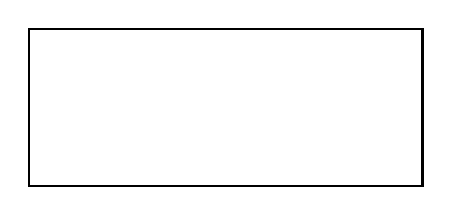
\begin{tikzpicture}
    \draw[thick] (0, 0) rectangle (5, 2);
\end{tikzpicture}
    \caption{Dual-mode circular waveguide filter. \cite{DMCWF-Dimensions}
    $W_C=43.87$ mm, $D_C=28.0$ mm, $L_B=43.87$ mm, $W_B=19.05$ mm, $H_B=9.525$ mm,
    $L_B=20.0$ mm, $W_S=10.05$ mm, $H_S=3.0$ mm, $W_A=2.0$ mm, $H_A=3.375$ mm,
    $L_A=2.825$ mm, thickness of all irises $2.0$ mm, screws half way up
    the cavity horizontal tuning screws with depth $3.82$ mm
    and coupling screws at angles $\pm 45^{\circ}$ with depth $3.57$ mm.}
    \label{fig:DMCWF}
\end{figure}

% Modeling process cite rubia

% Scattering coefficient

% Measurement procedure


\pagebreak
\section{Conclusion and outlook}
\label{sec:conclusion}

\pagebreak
\section{Appendix}
\label{sec:appendix}

\subsection{Detailed derivation for the weak formulation of the time-harmonic potential equation}
\label{subsec:derivation}

% !REMINDME: Levi-Civita tensor explanations.
The goal is to rewrite the curl-integral on the left-hand side of 
(\ref{equ:maxwell-weak-initial}):
\begin{equation}
    \int_{\Omega} (\nabla \times (\mu^{-1} \nabla \times \mathbf{u})) \cdot \mathbf{v} \label{equ:maxwell-weak-initial-LHS}
\end{equation}
In order to simplify the curls and apply the Gauss theorem, I first show
the following vector calculus identity:
\begin{fancybox}{Curl product rule}
    \begin{equation}
        (\nabla \times \mathbf{a}) \cdot \mathbf{b} = \nabla \cdot (\mathbf{a} \times \mathbf{b}) + \mathbf{a} \cdot (\nabla \times \mathbf{b}) \label{equ:vector-calculus} \\
    \end{equation}
\end{fancybox}
% !REMINDME: Appropriate spaces
where $\mathbf{a}$, $\mathbf{b}$ are vector-value functions. The completely
antisymmetric tensor $\varepsilon_{ijk}$, frequently referred to as the
Levi-Civita tensor, may be employed to rewrite the components of the
curl of a vector-function $\mathbf{a}$ as the sum
% !REMINDME: Maybe lemma and proof formatting
\begin{equation}
    (\nabla \times \mathbf{a})_k = \sum_i \sum_j \varepsilon_{ijk} \partial_i u_j
\end{equation}
where $\partial_i$ denotes the partial derivative with respect to the $i$-th coordinate
direction. This yields
\begin{align}
    (\nabla \times \mathbf{a}) \cdot \mathbf{b} &= \sum_k (\nabla \times \mathbf{a})_k b_k \notag \\ 
    &= \sum_k (\sum_i \sum_j \varepsilon_{ijk} \partial_i a_j) b_k \notag \\ 
    &= \sum_k \sum_i \sum_j \partial_i (\varepsilon_{ijk} a_j b_k) - \sum_k \sum_i \sum_j a_j (\varepsilon_{ijk} \partial_i b_k) \notag \\ 
    &= \sum_k \sum_i \sum_j \partial_i (\varepsilon_{jki} a_j b_k) - \sum_k \sum_i \sum_j a_j ((-\varepsilon_{ikj}) \partial_i b_k) \notag \\ 
    &= \sum_i \partial_i (\mathbf{a} \times \mathbf{b})_i + \sum_j u_j (\nabla \times \mathbf{b})_j \notag \\ 
    &= \nabla \cdot (\mathbf{a} \times \mathbf{b}) + \mathbf{a} \cdot (\nabla \times \mathbf{b}) \label{equ:curlidentity} 
\end{align}
by expressing the scalar product as a component-sum, using the product rule and
applying the symmetry and anti-symmetry properties of the Levi-Civita tensor.
Now the identity (\ref{equ:vector-calculus}) to (\ref{equ:maxwell-weak-initial-LHS})
together with Gauss' theorem gives
\begin{align}
    \int_{\Omega} (\nabla \times ({\mu^{-1} \nabla \times \mathbf{u}})) \cdot \mathbf{v} &=
    \int_{\Omega} \nabla \cdot (({\mu^{-1} \nabla \times \mathbf{u}}) \times \mathbf{v})
    + \int_{\Omega} ({\mu^{-1} \nabla \times \mathbf{u}}) \cdot (\nabla \times \mathbf{v}) \notag \\
    &= \int_{\partial \Omega} (({\mu^{-1} \nabla \times \mathbf{u}}) \times \mathbf{v}) \cdot \mathbf{n}
    + \int_{\Omega} ({\mu^{-1} \nabla \times \mathbf{u}}) \cdot (\nabla \times \mathbf{v}) \notag \\
\end{align}

For later convenience, the boundary integral can further be simplified using the
\begin{fancybox}{Commutative behavior of the scalar triple product}
    \begin{equation}
        (\mathbf{a} \times \mathbf{b}) \cdot \mathbf{c} = - (\mathbf{a} \times \mathbf{c}) \cdot \mathbf{b} \label{equ:vector-algebra}
    \end{equation}
\end{fancybox}
This identity follows immediately from a small manipulation with the Levi-Civita
tensor:
\begin{align}
    (\mathbf{a} \times \mathbf{b}) \cdot \mathbf{c} &= \sum_k (\sum_i \sum_j \varepsilon_{ijk} a_i b_j) c_k \notag \\
     &= \sum_j (\sum_i \sum_k (-\varepsilon_{ikj}) a_i c_k) b_j \notag \\ 
     &= - (\mathbf{a} \times \mathbf{c}) \cdot \mathbf{b} 
\end{align}
The boundary integral becomes 
\begin{equation}
    \int_{\partial \Omega} (({\mu^{-1} \nabla \times \mathbf{u}}) \times \mathbf{v}) \cdot \mathbf{n}
    = - \int_{\partial \Omega} (({\mu^{-1} \nabla \times \mathbf{u}}) \times \mathbf{n}) \cdot \mathbf{v}
\end{equation}

This concludes the short derivation, because now (\ref{equ:maxwell-weak-initial-LHS})
may be rewritten as
\begin{equation}
    - \int_{\partial \Omega} (({\mu^{-1} \nabla \times \mathbf{u}}) \times \mathbf{v}) \cdot \mathbf{n}
    + \int_{\Omega} ({\mu^{-1} \nabla \times \mathbf{u}}) \cdot (\nabla \times \mathbf{v})
\end{equation}

% 
\newpage
\bibliography{biblio.bib}

\end{document}